\chapter{Scattering, Renormalization, and Gauge Theory}

\section{Outline of QFT II}

\begin{enumerate}
\item The \(S\)-matrix:
\begin{itemize}
  \item bound states and resonances;
  \item implications of causality and unitarity;
  \item infrared divergence.
\end{itemize}

\item Renormalization Group:
\begin{itemize}
  \item BPHZ renormalizability;
  \item the 1PI effective action;
  \item improved perturbation theory, via the Gell--Mann--Low equation;
  \item Wilson--Polchinski renormalization group;
  \item \(\epsilon\)-expansion.
\end{itemize}

\item QCD:
\begin{itemize}
  \item quantization of non-Abelian gauge theory;
  \item BRST and BV formalisms;
  \item asymptotic freedom;
  \item OPE and deep inelastic scattering;
  \item \(1/N\) expansion;
  \item chiral symmetry breaking and the effective theory of pions;
  \item anomalies;
  \item instantons.
\end{itemize}
\end{enumerate}

\section{Recap of Some Basic Aspects of QFT}

We consider a \(\QM\) system with Hilbert space \(\mathcal H\) and
Poincare symmetry represented by a unitary operator \(U(\Lambda,a)\).
The group law is
\[
  U(\Lambda',a')U(\Lambda,a)
  =
  U(\Lambda'\Lambda,\Lambda'a+a').
\]
Infinitesimally,
\[
  U\!\left(\Lambda^\mu{}_\nu=\delta^\mu{}_\nu+\omega^\mu{}_\nu,
  a^\mu=\epsilon^\mu\right)
  =
  1-\ii\epsilon^\mu \widehat P_\mu
  +\frac{\ii}{2}\omega_{\rho\sigma}\widehat J^{\rho\sigma}.
\]

The energy-momentum operators are
\[
  \widehat P^\mu\equiv(\widehat P^0=\widehat H,\widehat P^i)
  =
  \int \dd^{D-1}\vec x\,T^{0\mu}(x),
\]
and the angular-momentum/boost generators are
\[
  \widehat J^{\mu\nu}
  =
  \int \dd^{D-1}\vec x\,
  \left[x^\mu T^{0\nu}(x)-(\mu\leftrightarrow\nu)\right].
\]
Here \(T^{\mu\nu}(x)\) is the stress-energy tensor.

Assume that the vacuum state \(\ket{\Omega}\) is Poincare-invariant,
\[
  \widehat P^\mu\ket{\Omega}
  =
  \widehat J^{\mu\nu}\ket{\Omega}
  =
  0.
\]
A local field operator \(\widehat\Phi_\alpha(x)\), where \(\alpha\) is a
Lorentz index, transforms as
\[
  U(\Lambda,a)\widehat\Phi_\alpha(x)U(\Lambda,a)^{-1}
  =
  \left(R(\Lambda)^{-1}\right)_\alpha{}^\beta
  \widehat\Phi_\beta(\Lambda x+a),
\]
where \(R(\Lambda)\) is the representation matrix of the Lorentz group
(or of its covering group).

Assuming that the Hilbert space is spanned by asymptotic states of
particles, in particular the one-particle state \(\ket{\vec k}\) obeys
\[
  \widehat P^i\ket{\vec k}=k^i\ket{\vec k},
  \qquad
  \widehat H\ket{\vec k}
  =
  \sqrt{\vec k^{\,2}+m^2}\,\ket{\vec k}
  =
  \omega_k\ket{\vec k}
\]
for some mass \(m\), with
\[
  \omega_k=\sqrt{\vec k^{\,2}+m^2}.
\]

A typical scalar field operator \(\widehat\phi(x)\), assuming one species
of scalar particle, has
\[
\begin{aligned}
  \widehat\phi(x)\ket{\Omega}
  &=
  \int \dd^{D-1}\vec k\,
  \ee^{-\ii\vec k\cdot\vec x+\ii\omega_k x^0}
  \left[
    \frac{Z_\phi}{(2\pi)^{D-1}}\frac{1}{2\omega_k}
  \right]^{1/2}
  \ket{\vec k}
\\
  &\quad
  +\int_{\mathrm{m.p.}}\dd\alpha\,
  \ee^{-\ii P_\alpha\cdot x}
  \bra{\alpha}\widehat\phi(0)\ket{\Omega}\ket{\alpha}.
\end{aligned}
\]

\subsection{Spectral Representation}

The spectral representation of the two-point Wightman function is
\[
  \bra{\Omega}\widehat\phi(x)\widehat\phi(y)\ket{\Omega}
  =
  \int_0^\infty \dd\mu^2\,\rho(\mu^2)\,
  \Delta_+(x-y;\mu^2),
\]
where
\[
  \Delta_+(x;\mu^2)
  =
  \int \frac{\dd^D k}{(2\pi)^{D-1}}\,
  \theta(k^0)\delta(k^2+\mu^2)\,\ee^{\ii k\cdot x}.
\]

The corresponding spectral representation of the time-ordered Green
function is
\[
  \bra{\Omega}T\widehat\phi(x)\widehat\phi(y)\ket{\Omega}
  =
  \int_0^\infty \dd\mu^2\,\rho(\mu^2)\,
  \Delta_F(x-y;\mu^2),
\]
with
\[
  \Delta_F(x;\mu^2)
  =
  -\ii\int \frac{\dd^D k}{(2\pi)^D}\,
  \frac{\ee^{\ii k\cdot x}}{k^2+\mu^2-\ii\epsilon}.
\]

For the Euclidean Green function,
\[
  \left\langle \phi(x^E)\phi(y^E)\right\rangle
  =
  \int_0^\infty \dd\mu^2\,\rho(\mu^2)\,
  \Delta_E(x^E-y^E;\mu^2),
\]
where
\[
  \Delta_E(x^E;\mu^2)
  =
  \int \frac{\dd^D k^E}{(2\pi)^D}\,
  \frac{\ee^{\ii k^E\cdot x^E}}{(k^E)^2+\mu^2}.
\]
The spectral density takes the form
\[
  \rho(\mu^2)
  =
  Z_\phi\delta(\mu^2-m^2)+\sigma(\mu^2),
\]
where \(\sigma\geq 0\) is supported at multiparticle invariant masses.

\begin{center}
\begin{tikzpicture}[>=Stealth,scale=1.05]
  \draw[->] (0,0) -- (5.7,0) node[right] {$\mu$};
  \draw[->] (0,0) -- (0,3.3) node[above] {$\rho$};
  \draw[blue,line width=1.1pt] (1.45,0) -- (1.45,2.95);
  \node[below] at (1.45,0) {$m$};
  \draw[blue,line width=1.1pt]
    (2.55,0) .. controls (3.0,1.55) and (3.35,2.05) .. (3.9,1.8)
    .. controls (4.45,1.55) and (4.75,0.92) .. (5.35,0.72);
  \node[below] at (2.55,0) {$2m$};
  \node[blue,align=left,anchor=west] at (3.6,2.55) {
    \(\geq0\), supported\\
    at m.p. inv. masses};
\end{tikzpicture}
\end{center}

The time-ordered and Euclidean Green functions are related by Wick
rotation:
\[
  x_a^0=\ee^{-\ii\alpha}\tau_a,
  \qquad
  \alpha:0\to\frac{\pi}{2},
  \qquad
  x_a^D=\tau_a.
\]

\begin{center}
\begin{tikzpicture}[>=Stealth,scale=1.0]
  \draw[->] (-3.7,0) -- (3.7,0) node[right] {$\operatorname{Re}x^0$};
  \draw[->] (0,-3.15) -- (0,3.15) node[above] {$-\operatorname{Im}x^0$};
  \draw[green!50!black,line width=1.2pt,->]
    (-3.05,-1.0) -- (2.25,0.45);
  \node[green!50!black,anchor=west] at (1.2,0.62) {time-ordered};
  \foreach \x/\lab in {-2.15/{x_n^0},-0.15/{x_2^0},0.95/{x_1^0}} {
    \fill[red] (\x,{0.25+0.13*\x}) circle (2.2pt);
    \node[red,below] at (\x,{0.25+0.13*\x}) {\(\lab\)};
  }
  \fill[purple] (0,2.12) circle (2.2pt) node[right] {\(\tau_1\)};
  \fill[purple] (0,1.32) circle (2.2pt) node[right] {\(\tau_2\)};
  \fill[purple] (0,-2.08) circle (2.2pt) node[right] {\(\tau_n\)};
  \node[purple,right] at (0.15,-2.75) {Euclidean};
  \draw[purple,dotted,line width=0.9pt] (0,1.0) -- (0,-1.8);
  \draw[orange,->,line width=1.0pt] (0.55,2.25) to[out=-35,in=120] (1.1,0.75);
  \draw[orange,->,line width=1.0pt] (-1.6,-2.0) to[out=55,in=210] (-0.35,-1.05);
\end{tikzpicture}
\end{center}

\subsection{Path Integral Representation}

The Lorentzian action is
\[
  S=\int \dd^D x\,\mathcal L[\phi],
\]
whereas the Euclidean action is
\[
  S^E=\int \dd^D x^E\,\mathcal L^E[\phi],
  \qquad
  \mathcal L^E[\phi]
  =
  -\mathcal L[\phi]\Big|_{x^0\to-\ii x^D,\;\vec x=\vec x^E}.
\]
The Euclidean correlators are represented by
\[
  \left\langle \phi(x_1^E)\cdots\phi(x_n^E)\right\rangle
  =
  \frac{1}{Z}\int [D\phi]\,
  \ee^{-S^E[\phi]}\,
  \phi(x_1^E)\cdots\phi(x_n^E),
\]
while the time-ordered correlators are represented by
\[
  \bra{\Omega}T\widehat\phi(x_1)\cdots\widehat\phi(x_n)\ket{\Omega}
  =
  \frac{1}{Z}\int [D\phi]\,
  \ee^{\ii S[\phi]}\,
  \phi(x_1)\cdots\phi(x_n).
\]

\section{The S-Matrix and LSZ}

At early or late times, a generic state admits a particle
interpretation:

\begin{center}
\begin{tikzpicture}[>=Stealth,scale=1.0]
  \draw[->] (-4.0,-1.8) -- (-4.0,2.2) node[above] {time};
  \draw[orange,dashed,line width=0.8pt] (-1.8,-1.1) -- (2.2,-1.1);
  \draw[green!50!black,dashed,line width=0.8pt] (-1.8,1.15) -- (2.2,1.15);
  \node[orange,anchor=west] at (2.35,-1.1) {in-basis \(\ket{\alpha}^{\mathrm{in}}\)};
  \node[green!50!black,anchor=west] at (2.35,1.15) {out-basis \(\ket{\beta}^{\mathrm{out}}\)};
  \draw[blue,line width=1.1pt] (0,0) ellipse (1.18 and 0.75);
  \foreach \x in {-0.65,0,0.65} {
    \draw[orange,line width=1.0pt,->] (\x,-1.75) -- ({0.45*\x},-0.62);
  }
  \foreach \x in {-0.75,0,0.75} {
    \draw[green!50!black,line width=1.0pt,->] ({0.45*\x},0.62) -- (\x,1.75);
  }
  \node at (0,-2.2) {\(S\)-matrix};
\end{tikzpicture}
\end{center}

The \(S\)-matrix is
\[
  S_{\beta\alpha}\equiv{}^{\mathrm{out}}\!\bra{\beta}\alpha\rangle^{\mathrm{in}}.
\]
Equivalently,
\[
  \ket{\alpha}^{\mathrm{in}}
  =
  \sum_{\beta}S_{\beta\alpha}\ket{\beta}^{\mathrm{out}},
\]
where the measure is such that
\[
  \sum_{\beta}\ket{\beta}^{\mathrm{out}}{}^{\mathrm{out}}\!\bra{\beta}=1.
\]

The asymptotic in/out-states are tied to local field operators via
\[
  \ket{\phi_{f_1},\ldots,\phi_{f_n}}^{\mathrm{out/in}}
  =
  \lim_{T\to\pm\infty}
  \widehat\phi_{f_1}^{(T)}\cdots
  \widehat\phi_{f_n}^{(T)}\ket{\Omega},
\]
where
\[
  \widehat\phi_f=\int \dd^D x\,f(x)\widehat\phi(x),
\]
such that
\[
  f(x)\equiv
  \int \frac{\dd^D k}{(2\pi)^D}\,\widetilde f(k)\,\ee^{\ii k\cdot x},
\]
with \(\widetilde f(k)\) supported near the one-particle mass-shell.
The function \(f^{(T)}(x)\) is the transform of \(\widetilde f(\vec k)\)
defined by
\[
  f^{(T)}(x)
  =
  \int \frac{\dd^{D-1}\vec k}{(2\pi)^D}\,
  \widetilde f(\vec k)\,
  \ee^{\ii(k^0-\omega_k)T+\ii k\cdot x}.
\]
In particular,
\[
  \widehat\phi_{f^{(T)}}\ket{\Omega}
  =
  \widehat\phi_f\ket{\Omega},
\]
consisting only of one-particle states.

The LSZ reduction formula follows from this construction and the cluster
property of Green functions.

\subsection{Cluster Property and LSZ}

The cluster property of \(S\)-matrix elements says
\[
  S(\beta|\alpha)
  =
  \sum_{\substack{\alpha=\coprod_I\alpha_I\\ \beta=\coprod_I\beta_I}}
  \prod_I S^{\mathrm{conn}}(\beta_I|\alpha_I).
\]

The LSZ formula states that connected \(S\)-matrix elements, or
``scattering amplitudes,'' are related to the Fourier transform of
connected time-ordered Green functions:
\[
\begin{aligned}
  &S^{\mathrm{conn}}(\vec k_1,\ldots,\vec k_n
  |-\vec k'_1,\ldots,-\vec k'_m)
\\
  &=
  \prod_{i=1}^{n}
  \left[Z_\phi(2\pi)^{D-1}2\omega_{k_i}\right]^{-1/2}
  \prod_{j=1}^{m}
  \left[Z_\phi(2\pi)^{D-1}2\omega_{k'_j}\right]^{-1/2}
\\
  &\quad\times
  \lim_{\substack{k_i^0\to\omega_{k_i}\\ k_j^{\prime 0}\to-\omega_{k'_j}}}
  \prod_i \ii(k_i^2+m^2)
  \prod_j \ii(k_j^{\prime 2}+m^2)\,
  \widetilde G^{\mathrm{conn}}(k_1,\ldots,k_n,k'_1,\ldots,k'_m),
\end{aligned}
\]
where
\[
  \widetilde G^{\mathrm{conn}}
  =
  \int \dd^D x_1\cdots\,
  \ee^{-\ii k_1\cdot x_1-\cdots}
  G^{\mathrm{conn}}(x_1,\ldots,x'_1,\ldots),
\]
and the Green function is time-ordered.

We use the convention
\[
\begin{aligned}
  &S^{\mathrm{conn}}(\vec k_1,\ldots,\vec k_n
  |-\vec k'_1,\ldots,-\vec k'_m)
\\
  &\equiv
  \ii(2\pi)^D
  \delta^D(k_1+\cdots+k_n-k'_1-\cdots-k'_m)\,
  \mathcal M(\vec k_1,\ldots,\vec k_n|\vec k'_1,\ldots,\vec k'_m),
\end{aligned}
\]
where
\[
  \mathcal M
  =
  \prod_i\frac{1}{(2\pi)^{(D-1)/2}\sqrt{2\omega_{k_i}}}
  \prod_j\frac{1}{(2\pi)^{(D-1)/2}\sqrt{2\omega_{k'_j}}}\,
  \mathcal A(k_1,\ldots,k_n|k'_1,\ldots,k'_m),
\]
and \(\mathcal A\) is Lorentz-invariant.

\section{Bound States from a Simple Exchange Amplitude}

Consider two scalar fields \(\phi_1,\phi_2\) with
\[
  \mathcal L
  =
  -\frac12(\partial_\mu\phi_1)^2-\frac12 m_1^2\phi_1^2
  -\frac12(\partial_\mu\phi_2)^2-\frac12 m_2^2\phi_2^2
  -\frac12 g\phi_1^2\phi_2.
\]
The Lorentzian Feynman rules are
\[
  \phi_1\text{ propagator:}\quad
  \frac{-\ii}{k^2+m_1^2-\ii\epsilon},
  \qquad
  \phi_2\text{ propagator:}\quad
  \frac{-\ii}{k^2+m_2^2-\ii\epsilon},
\]
and the cubic vertex is
\[
  \phi_1\phi_1\phi_2:\qquad -\ii g.
\]

Consider the \(2\to2\) scattering amplitude of the particle created by
\(\phi_1\):
\[
  \ii\mathcal A(k_3,k_4;k_1,k_2)
  =
  \ii\mathcal A_{\mathrm{tree}}+O(g^4).
\]

\begin{center}
\begin{tikzpicture}[>=Stealth,scale=1.0,
  scalar/.style={line width=0.8pt},
  exch/.style={dash pattern=on 3pt off 2pt,line width=0.8pt}
]
  \begin{scope}[xshift=-3.6cm]
    \draw[scalar] (-1,-0.8) -- (0,0) -- (-1,0.8);
    \draw[scalar] (0,0) -- (1,0.8);
    \draw[scalar] (0,0) -- (1,-0.8);
    \draw[exch] (-0.25,0) -- (0.65,0);
  \end{scope}
  \node at (-1.65,0) {\(+\)};
  \begin{scope}[xshift=0cm]
    \draw[scalar] (-1,-0.8) -- (0,-0.2) -- (1,-0.8);
    \draw[scalar] (-1,0.8) -- (0,0.2) -- (1,0.8);
    \draw[exch] (0,-0.2) -- (0,0.2);
  \end{scope}
  \node at (1.75,0) {\(+\)};
  \begin{scope}[xshift=3.6cm]
    \draw[scalar] (-1,-0.8) -- (0,0) -- (1,0.8);
    \draw[scalar] (-1,0.8) -- (0,0) -- (1,-0.8);
    \draw[exch] (-0.25,-0.25) -- (0.45,0.45);
  \end{scope}
\end{tikzpicture}
\end{center}

At tree level,
\[
  \ii\mathcal A_{\mathrm{tree}}
  =
  (-\ii g)^2
  \frac{-\ii}{(k_1+k_2)^2+m_2^2-\ii\epsilon}
  +(k_2\to-k_3)+(k_2\to-k_4).
\]
Define the Mandelstam variables
\[
  s\equiv-(k_1+k_2)^2,
  \qquad
  t\equiv-(k_1-k_3)^2,
  \qquad
  u\equiv-(k_1-k_4)^2.
\]
Then
\[
  \ii\mathcal A_{\mathrm{tree}}
  =
  \ii g^2\left(
    \frac{1}{-s+m_2^2-\ii\epsilon}
    +
    \frac{1}{-t+m_2^2-\ii\epsilon}
    +
    \frac{1}{-u+m_2^2-\ii\epsilon}
  \right).
\]
We will spend a little time interpreting this simple-looking result.

In terms of the center-of-mass total energy \(E\) and scattering angle
\(\theta\),
\[
  s=E^2,
  \qquad
  t=-\frac{E^2-4m_1^2}{2}(1-\cos\theta),
  \qquad
  u=-\frac{E^2-4m_1^2}{2}(1+\cos\theta).
\]
The physical mass \(m_{1*}\) of the particle may differ from \(m_1\) at
higher orders in \(g\), but we will ignore this for now.

Case I: \(m_2<2m_1\). For physically admissible kinematics,
\[
  E\geq 2m_1
  \quad\Longrightarrow\quad
  s>m_2^2
  \quad\text{and}\quad
  t,u<0.
\]
Thus \(\mathcal A_{\mathrm{tree}}\) is always finite. If we analytically
continue \(\mathcal A_{\mathrm{tree}}\) on the complex \(E\)-plane, or
\(s\)-plane, we find a pole at
\[
  E=m_2<2m_1.
\]
Interpretation: the particle of mass \(m_2\) is a bound state of a pair
of particles of mass \(m_1\).

\subsection{A Nonrelativistic Scattering Analogy}

Comparison with a simple non-relativistic quantum-mechanics model:
scattering in one dimension.  Take
\[
  H=\frac{p^2}{2m}+V(x),
  \qquad
  V(x\to\infty)=0.
\]

\begin{center}
\begin{tikzpicture}[>=Stealth,scale=0.92]
  \draw[->,line width=0.7pt] (0,0) -- (5.8,0) node[right] {\(x\)};
  \draw[->,line width=0.7pt] (0,-2.0) -- (0,2.4) node[above] {\(V(x)\)};
  \draw[blue,line width=1.0pt]
    (0.15,2.1) .. controls (0.45,-1.9) and (0.95,-1.95) .. (1.35,-0.2)
    .. controls (1.65,0.95) and (2.05,0.9) .. (2.45,0.1)
    .. controls (2.95,-0.85) and (3.4,0.45) .. (3.95,0.85)
    .. controls (4.5,0.6) and (4.75,0.2) .. (5.45,0.04);
  \draw[orange,line width=1.0pt]
    (0.55,0.28) .. controls (0.95,0.7) and (1.18,0.75) .. (1.45,0.2)
    .. controls (1.75,-0.25) and (2.0,-0.05) .. (2.3,0.28)
    .. controls (2.62,0.65) and (2.88,0.3) .. (3.15,-0.2);
  \draw[green!55!black,line width=1.0pt]
    (1.05,-1.45) .. controls (1.6,-1.25) and (1.85,0.25) .. (2.45,0.15)
    .. controls (3.0,0.03) and (3.15,-1.25) .. (3.72,-1.33);
  \node[blue] at (1.05,1.75) {\(V(x)\)};
  \node[orange] at (1.55,0.98) {resonance};
  \node[purple,align=center] at (4.42,1.15) {scattering\\wave function};
  \node[green!55!black,align=center] at (1.45,-1.75) {bound\\state};
\end{tikzpicture}
\end{center}

In the asymptotic region \(x\to\infty\), a scattering wave function takes
the form
\[
  \text{``in-state''}\qquad
  \psi^{\mathrm{in}}_k(x)
  \sim
  \ee^{-\ii kx}+S(k)\ee^{\ii kx}.
\]
Here \(S(k)\) is the scattering amplitude, analogous to a partial-wave
amplitude in higher dimensions.  The corresponding out-state is
\[
  \psi^{\mathrm{out}}_k(x)
  =
  (S(k))^{-1}\psi^{\mathrm{in}}_k(x)
  \sim
  (S(k))^{-1}\ee^{-\ii kx}+\ee^{\ii kx},
\]
with
\[
  k=\sqrt{2mE}
  \qquad
  \text{(assuming \(V(\infty)=0\)).}
\]
A bound state, on the other hand, has asymptotic wave function
\[
  \psi(x)\sim \ee^{-\alpha x},
  \qquad x\to\infty,
\]
where
\[
  \alpha=\sqrt{-2mE}>0
  \qquad
  (E<0).
\]

What is the relation between \(S(k)\) and the bound states?  If we do
not impose the normalizability of the wave function in the asymptotic
region \(x\to\infty\), we can analytically continue
\(\psi_k^{\mathrm{out}}\) as a solution to the Schrödinger equation at
complex \(k\).  Under
\[
  k\to \ii\alpha,
\]
\(\psi_k^{\mathrm{out}}\) becomes
\[
  \psi^{\mathrm{out}}_{\ii\alpha}(x)
  \sim
  (S(\ii\alpha))^{-1}\ee^{\alpha x}+\ee^{-\alpha x}.
\]
The growing term must vanish for a bound state.  Thus
\[
  \text{bound state}
  \quad\Longleftrightarrow\quad
  \text{pole of \(S(k)\) at \(k=\ii\alpha\), \(\alpha>0\).}
\]

\begin{center}
\begin{tikzpicture}[>=Stealth,scale=0.92]
  \begin{scope}
    \draw[black,line width=0.7pt] (-0.1,-1.6) rectangle (4.2,2.2);
    \draw[->,blue,line width=1pt] (1.45,0) -- (4.0,0) node[below] {\(k\geq0\)};
    \node[below] at (1.45,0) {\(0\)};
    \node[anchor=west] at (0.15,1.85) {cplx \(k\)};
    \fill[red] (1.45,0.85) circle (2.2pt) node[left] {\(\ii\alpha_1\)};
    \fill[red] (1.45,1.55) circle (2.2pt) node[left] {\(\ii\alpha_2\)};
    \node[purple] at (2.52,0.72) {\(\leftarrow\)};
  \end{scope}
  \begin{scope}[xshift=5.25cm]
    \draw[black,line width=0.7pt] (-0.1,-1.6) rectangle (4.2,2.2);
    \draw[->,blue,line width=1pt] (1.45,0) -- (4.0,0) node[below] {\(E\geq0\)};
    \node[below] at (1.45,0) {\(0\)};
    \node[anchor=west] at (0.15,1.85) {cplx \(E\)};
    \node at (1.5,2.45) {\(E=\dfrac{k^2}{2m}\)};
    \fill[red] (0.55,0) circle (2.2pt);
    \fill[red] (1.0,0) circle (2.2pt);
    \draw[->,purple,line width=1pt]
      (2.9,0.05) .. controls (3.05,1.35) and (1.05,1.55) .. (0.95,0.12);
    \node[orange,align=center] at (0.8,-0.72) {bound\\states};
  \end{scope}
  \node at (4.72,0.5) {\(\longmapsto\)};
\end{tikzpicture}
\end{center}

The precise analog of this in QFT is the bound-state pole in a
partial-wave amplitude.  Recall the relation between the two
\((\)scalar\()\)-particle plane-wave basis and partial-wave basis in the
center-of-mass frame, in the \(D=4\) case:
\[
\begin{aligned}
  &\braket{\vec k_1,\vec k_2}{E,\vec P=0,\ell,m}
\\
  &\quad =
  \delta^3(\vec k_1+\vec k_2)\,
  \delta(\omega_{\vec k_1}+\omega_{\vec k_2}-E)\,
  \mathcal N(E)\,
  Y_{\ell m}(\hat k_1),
\end{aligned}
\]
where, for identical particles,
\[
  \mathcal N(E)
  =
  \sqrt{\frac{2E}{|\vec k_1|\omega_{\vec k_1}\omega_{\vec k_2}}}.
\]
The \(S\)-matrix acts diagonally in angular momentum, up to inelastic
channels:
\[
  \ket{E,\ell,m}^{\mathrm{in}}
  =
  S_\ell(E)\ket{E,\ell,m}^{\mathrm{out}}
  +\text{inelastic}.
\]
The scattering amplitude is related to the partial-wave \(S\)-matrix by
\[
  \ii(2\pi)^4\mathcal M
  =
  \mathcal N(E)^2\frac{1}{4\pi}
  \sum_{\ell=0}^{\infty}
  (2\ell+1)P_\ell(\cos\theta)\bigl(S_\ell(E)-1\bigr),
\]
with only even \(\ell\) contributing in the identical-particle channel.
Equivalently,
\[
\begin{aligned}
  \ii\mathcal A(s,t)
  &=
  \ii(2\pi)^6 E^2\mathcal M
\\
  &=
  \frac{8\pi E}{k}
  \sum_{\ell=0}^{\infty}
  (2\ell+1)P_\ell(\cos\theta)\bigl(S_\ell(E)-1\bigr),
\end{aligned}
\]
where
\[
  E=\sqrt{4(k^2+m^2)}.
\]
A spin-\(\ell\) bound-state particle of mass \(M\) would correspond to a
pole of \(S_\ell(E)\) at
\[
  E=M<2m.
\]
We have seen that \(\phi_2\) gives rise to a pole in the \(s\)-wave
\((\ell=0)\) amplitude.

An example of a spin-one bound state: in scalar QED, particle-antiparticle
scattering,
\[
  \mathcal A\propto
  \frac{(p_1-p_2)^\mu(p_3-p_4)_\mu}{s}
  =
  \frac{4k^2\cos\theta}{s}.
\]
Since
\[
  P_1(\cos\theta)=\cos\theta,
\]
there is a pole of \(S_{\ell=1}\) at \(s=0\).  The photon can be viewed
as a bound state.

\subsection{Unstable Particles and Resonances}

Back to \(\phi_1\phi_1\to\phi_1\phi_1\) scattering.  Case II:
\[
  m_2>2m_1.
\]
The amplitude has a pole at
\[
  s=m_2^2,
\]
now in the physically admissible region.  Therefore
\(\mathcal A_{\mathrm{tree}}\), or \(S_{\ell=0}^{\mathrm{tree}}(E)\),
diverges at \(E=m_2\).  But unitarity demands
\[
  |S_{\ell=0}(E)|\leq 1.
\]
Is there a contradiction?

Intuition: when \(m_2>2m_1\), the ``particle'' created by \(\phi_2\) is
unstable against decay into a pair of \(\phi_1\)-particles; there is no
stable particle of mass near \(m_2\), but rather a resonance.

What is the signature of a resonance in \(\mathcal A\) or \(S_\ell(E)\)?
Let us revisit the simple NRQM model of one-dimensional scattering.

\begin{center}
\begin{tikzpicture}[>=Stealth,scale=0.9]
  \draw[->,line width=0.7pt] (0,0) -- (5.8,0) node[right] {\(x\)};
  \draw[->,line width=0.7pt] (0,-1.65) -- (0,2.05) node[above] {\(V(x)\)};
  \draw[blue,line width=1pt]
    (0.25,1.7) .. controls (0.45,-1.0) and (0.95,-1.55) .. (1.35,-0.15)
    .. controls (1.72,0.95) and (2.05,0.8) .. (2.4,0.12)
    .. controls (3.0,-0.8) and (3.8,0.15) .. (5.25,0.05);
  \draw[orange,line width=1pt]
    (0.75,0.28) .. controls (1.05,0.65) and (1.25,0.7) .. (1.48,0.18)
    .. controls (1.72,-0.25) and (2.0,0.05) .. (2.28,0.28)
    .. controls (2.7,0.62) and (3.25,0.25) .. (4.95,-0.15);
  \foreach \x in {1.2,1.8,2.6,3.7,4.35}
    \draw[->,brown,line width=0.8pt] (\x,0.15) -- ++(0,-0.45);
  \node[orange,align=center] at (0.9,0.95) {resonance\\state};
  \draw[->,red,line width=1pt] (4.1,1.0) -- (4.95,1.0);
  \node[red,align=left] at (5.85,1.0) {outgoing flux\\no incoming flux};
  \node[brown,align=left,anchor=west] at (4.35,-0.55)
    {wave function decays\\in time};
\end{tikzpicture}
\end{center}

The wave function of a resonance ``state'' that decays uniformly in time
is necessarily non-normalizable, due to conservation of probability.
Consider once again the out-state wave function, analytically continued
to complex
\[
  k=\sqrt{2mE}.
\]
In the asymptotic region,
\[
  \psi^{\mathrm{out}}_k(x,t)
  \sim
  (S(k))^{-1}\ee^{-\ii kx-\ii Et}
  +
  \ee^{\ii kx-\ii Et}.
\]
Suppose \(S(k)\) has a pole at \(k_*\), with
\[
  E_*=\frac{k_*^2}{2m}=\omega-\ii\gamma,
  \qquad
  \gamma>0,
\]
where \(\gamma\) is the decay width.  Then
\[
  \psi^{\mathrm{out}}_{k_*}(x,t)
  \sim
  \ee^{\ii k_*x-\ii\omega t-\gamma t}
\]
in the asymptotic region, with
\[
  k_*=\sqrt{2m(\omega-\ii\gamma)},
  \qquad
  \omega>0.
\]

\begin{center}
\begin{tikzpicture}[>=Stealth,scale=0.9]
  \begin{scope}
    \draw[black,line width=0.7pt] (-0.1,-1.8) rectangle (4.35,2.25);
    \node[anchor=west] at (0.15,1.9) {cplx \(k\)-plane};
    \draw[dashed,green!60!black,line width=0.8pt] (0.15,0) -- (1.45,0);
    \draw[->,blue,line width=1pt] (1.45,0) -- (4.1,0) node[below] {\(k\geq0\)};
    \node[below] at (1.45,0) {\(0\)};
    \fill[red] (1.45,0.75) circle (2.2pt);
    \fill[red] (1.45,1.25) circle (2.2pt);
    \node[red,align=center] at (0.75,1.15) {bound\\state\\poles};
    \fill[orange] (2.0,-0.75) circle (2.1pt);
    \fill[orange] (2.75,-0.9) circle (2.1pt);
    \fill[orange] (3.5,-1.0) circle (2.1pt);
    \node[orange,align=center] at (2.85,-1.45) {resonance\\poles};
    \draw[->,purple,line width=1pt]
      (2.75,0.08) .. controls (2.75,-0.25) and (2.35,-0.42) .. (2.05,-0.7);
    \draw[->,green!55!black,line width=1pt]
      (1.6,0.08) .. controls (1.0,0.6) and (0.82,0.15) .. (1.36,0.02);
  \end{scope}
  \begin{scope}[xshift=5.25cm]
    \draw[black,line width=0.7pt] (-0.1,-1.8) rectangle (4.35,2.25);
    \node[anchor=west] at (0.15,1.9) {cplx \(E\)-plane};
    \draw[decorate,decoration={snake,amplitude=0.55mm,segment length=2.7mm},
      blue,line width=1pt] (1.4,0) -- (4.1,0);
    \node[below] at (1.45,0) {\(0\)};
    \node[blue] at (3.7,0.28) {\(E>0\)};
    \fill[red] (0.75,0) circle (2.2pt);
    \fill[red] (1.15,0) circle (2.2pt);
    \draw[->,purple,line width=1pt]
      (3.4,0.12) .. controls (3.2,1.15) and (0.95,1.15) .. (0.92,0.12);
    \draw[->,green!55!black,line width=1pt]
      (1.05,0.05) .. controls (0.65,-0.75) and (1.65,-0.9) .. (1.65,-0.05);
    \fill[orange] (2.2,-0.78) circle (2.1pt);
    \fill[orange] (3.3,-1.2) circle (2.1pt);
    \node[orange,align=center,font=\small] at (2.9,-1.05)
      {resonance poles\\are on\\``2nd sheet''};
  \end{scope}
\end{tikzpicture}
\end{center}

\subsection{Self-Energy and the Decay Width}

Back to \(\phi_1\phi_1\to\phi_1\phi_1\) scattering.  We need to take
into account the self-energy of \(\phi_2\) to account for the decay
width of the resonance.

\begin{center}
\begin{tikzpicture}[>=Stealth,scale=0.92,
  one/.style={line width=0.8pt},
  two/.style={dash pattern=on 3pt off 2pt,line width=0.8pt},
  blob/.style={draw,fill=gray!20,circle,minimum size=0.68cm,inner sep=0pt}
]
  \begin{scope}
    \draw[one] (-1.3,0.8) -- (-0.45,0.15);
    \draw[one] (-1.3,-0.8) -- (-0.45,-0.15);
    \draw[two] (-0.45,0) -- (0.05,0);
    \node[blob] at (0.45,0) {};
    \draw[two] (0.8,0) -- (1.3,0);
    \draw[one] (1.3,0.15) -- (2.15,0.8);
    \draw[one] (1.3,-0.15) -- (2.15,-0.8);
    \node at (-1.55,0.9) {\(\phi_1\)};
    \node at (-1.55,-0.9) {\(\phi_1\)};
    \node at (2.35,0.9) {\(\phi_1\)};
    \node at (2.35,-0.9) {\(\phi_1\)};
    \node at (0.45,0.58) {\(\phi_2\)};
  \end{scope}
  \node[blue,align=center] at (0,-1.55)
    {need to take into account the self-energy of \(\phi_2\)\\
    to account for the decay width of the resonance};
\end{tikzpicture}
\end{center}

The dressed \(\phi_2\) propagator is obtained from a geometric series of
one-particle-irreducible insertions:
\[
  \frac{-\ii}{k^2+m_2^2-\ii\epsilon-\Sigma(k)}.
\]
Diagrammatically,
\[
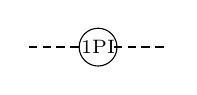
\begin{tikzpicture}[baseline=-0.45ex,scale=0.8,
  two/.style={dash pattern=on 3pt off 2pt,line width=0.8pt},
  blob/.style={draw,circle,minimum size=0.48cm,inner sep=0pt}]
  \draw[two] (-1.1,0) -- (-0.25,0);
  \node[blob] at (0,0) {\scriptsize 1PI};
  \draw[two] (0.25,0) -- (1.1,0);
\end{tikzpicture}
\quad = \quad
\begin{tikzpicture}[baseline=-0.45ex,scale=0.8,
  two/.style={dash pattern=on 3pt off 2pt,line width=0.8pt}]
  \draw[two] (-1.1,0) -- (1.1,0);
\end{tikzpicture}
\quad + \quad
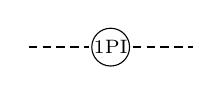
\begin{tikzpicture}[baseline=-0.45ex,scale=0.8,
  two/.style={dash pattern=on 3pt off 2pt,line width=0.8pt},
  blob/.style={draw,circle,minimum size=0.48cm,inner sep=0pt}]
  \draw[two] (-1.3,0) -- (-0.35,0);
  \node[blob] at (0,0) {\scriptsize 1PI};
  \draw[two] (0.35,0) -- (1.3,0);
\end{tikzpicture}
\quad + \quad
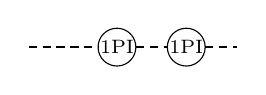
\begin{tikzpicture}[baseline=-0.45ex,scale=0.8,
  two/.style={dash pattern=on 3pt off 2pt,line width=0.8pt},
  blob/.style={draw,circle,minimum size=0.48cm,inner sep=0pt}]
  \draw[two] (-1.65,0) -- (-0.55,0);
  \node[blob] at (-0.25,0) {\scriptsize 1PI};
  \draw[two] (0.05,0) -- (0.55,0);
  \node[blob] at (0.85,0) {\scriptsize 1PI};
  \draw[two] (1.15,0) -- (1.65,0);
\end{tikzpicture}
\quad +\cdots .
\]

At one loop,
\[
\begin{aligned}
  \ii\Sigma(k)
  &=
  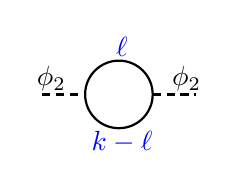
\begin{tikzpicture}[baseline=-0.55ex,scale=0.78,
    two/.style={dash pattern=on 3pt off 2pt,line width=0.8pt},
    one/.style={line width=0.8pt}]
    \draw[two] (-1.25,0) -- (-0.55,0);
    \draw[two] (0.55,0) -- (1.25,0);
    \draw[one] (0,0) circle (0.55);
    \node at (-1.1,0.25) {\(\phi_2\)};
    \node at (1.1,0.25) {\(\phi_2\)};
    \node[blue] at (0.05,0.78) {\(\ell\)};
    \node[blue] at (0.05,-0.78) {\(k-\ell\)};
  \end{tikzpicture}
  +O(g^4)
\\
  &=
  \frac{(-\ii g)^2}{2}
  \int\frac{\dd^D\ell}{(2\pi)^D}\,
  \frac{-\ii}{\ell^2+m_1^2-\ii\epsilon}\,
  \frac{-\ii}{(k-\ell)^2+m_1^2-\ii\epsilon}.
\end{aligned}
\]
Using a Feynman parameter,
\[
  \ii\Sigma(k)
  =
  \frac{g^2}{2}
  \int\frac{\dd^D\ell}{(2\pi)^D}\int_0^1\dd x\,
  \frac{1}{
  \left[\ell^2(1-x)+(k-\ell)^2x+m_1^2-\ii\epsilon\right]^2}.
\]
First shift
\[
  \ell^\mu\to \ell^\mu+xk^\mu,
\]
then Wick rotate
\[
  \ell^0=\ii\ell_E^0.
\]
This gives
\[
  \ii\Sigma(k)
  =
  \ii\frac{g^2}{2}
  \int_0^1\dd x
  \int\frac{\dd^D\ell_E}{(2\pi)^D}\,
  \frac{1}{
  \left[\ell_E^2+k^2x(1-x)+m_1^2-\ii\epsilon\right]^2}.
\]

Specialize to the \(D=4\) case, regularized with a cutoff
\[
  |\ell_E|<\Lambda.
\]
A more systematic regularization scheme is dimensional regularization,
but the simple momentum cutoff scheme suffices for our discussion at
one-loop order.  Then
\[
  \ii\Sigma(k)
  =
  \ii\frac{g^2}{32\pi^2}
  \int_0^1\dd x
  \left[
    \log\frac{\Lambda^2}{k^2x(1-x)+m_1^2-\ii\epsilon}
    -1+O(\Lambda^{-2})
  \right].
\]

The \(k\)-independent terms, which come with the UV divergence, can be
absorbed into a redefinition of the mass parameter \(m_2\).  Equivalently,
\[
  \left(m_2^{\mathrm{bare}}\right)^2
  =
  \left(m_2^R\right)^2+\delta m_2^2,
\]
where \(m_2^R\) is finite, and the counterterm \(\delta m_2^2\) serves
to cancel the \(k\)-independent UV divergence in \(\Sigma(k)\).
We can write
\[
  \Sigma(k)=\Sigma^R(k)+\delta m_2^2,
\]
where
\[
  \Sigma^R(k)
  =
  -\frac{g^2}{32\pi^2}
  \int_0^1\dd x\,
  \log\frac{k^2x(1-x)+m_1^2-\ii\epsilon}{m_1^2}.
\]
Thus the renormalized dressed propagator is
\[
  \frac{-\ii}{k^2+\left(m_2^R\right)^2-\ii\epsilon-\Sigma^R(k)}.
\]

Let us examine the analytic and singularity structure of the corresponding
contribution to \(\phi_1\phi_1\) scattering, with momentum
\(k_1+k_2\) carried by the dressed \(\phi_2\) line.  Its contribution to
the scattering amplitude \(\mathcal A\) is
\[
  \mathcal A
  =
  \frac{g^2}{
    -s+\left(m_2^R\right)^2-\ii\epsilon
    +
    \frac{g^2}{32\pi^2}
    \int_0^1\dd x\,
    \log\left[1-\frac{s\,x(1-x)}{m_1^2}-\ii\epsilon\right]
  }.
\]
For \(0\leq x\leq1\),
\[
  0\leq x(1-x)\leq\frac14,
\]
so the argument of the logarithm is negative in the physical region
\[
  s\in[4m_1^2,\infty).
\]
The branch choice is read off from the \(\ii\epsilon\) prescription.

More fundamentally, the value of \(\Sigma(k)\) at real Lorentzian \(k^0\)
is determined by the Wick rotation and analytic continuation relating
the Euclidean Green function \(G_E\) to the time-ordered Green function
\(G\).  For real
\[
  k^0\to \sqrt{\vec k^2+M^2},
\]
\(\Sigma(k)\) is given by analytic continuation from \(k^0\in \ii\mathbb R\)
to the positive real \(k^0\)-axis from above.

\begin{center}
\begin{tikzpicture}[>=Stealth,scale=0.9]
  \draw[->,line width=0.7pt] (-2.2,0) -- (3.3,0) node[right] {\(\operatorname{Re} k^0\)};
  \draw[->,green!55!black,line width=1pt] (0,-2.2) -- (0,2.3)
    node[above] {\(\operatorname{Im} k^0\)};
  \draw[red,decorate,decoration={snake,amplitude=0.5mm,segment length=2.5mm},
    line width=0.8pt] (-2.0,0) -- (-1.1,0);
  \draw[red,decorate,decoration={snake,amplitude=0.5mm,segment length=2.5mm},
    line width=0.8pt] (1.2,0) -- (3.0,0);
  \draw[->,orange,line width=1pt]
    (1.1,1.35) .. controls (2.0,1.25) and (2.45,0.85) .. (2.6,0.15);
  \node[orange] at (2.25,1.6) {Wick};
  \node[blue] at (3.05,-0.28) {Re};
  \node[green!55!black] at (0.32,2.1) {Im};
  \node[align=left,anchor=west,font=\small] at (3.35,1.05)
    {analytic continuation from \(k^0\in \ii\mathbb R\)\\
    to positive real \(k^0\)-axis\\
    from above};
\end{tikzpicture}
\end{center}

On the complex \(s\)-plane:
\[
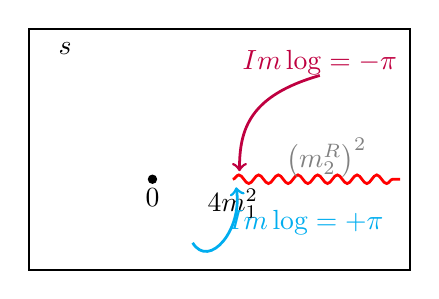
\begin{tikzpicture}[baseline=-0.55ex,scale=0.85]
  \draw[black,line width=0.7pt] (-0.1,-1.35) rectangle (5.6,2.25);
  \node[anchor=west] at (0.2,1.95) {\(s\)};
  \fill (1.75,0) circle (2pt) node[below] {\(0\)};
  \draw[red,decorate,decoration={snake,amplitude=0.55mm,segment length=2.5mm},
    line width=1pt] (2.95,0) -- (5.45,0);
  \node[below] at (2.95,0) {\(4m_1^2\)};
  \node[gray] at (4.35,0.32) {\(\left(m_2^R\right)^2\)};
  \draw[->,purple,line width=1pt]
    (4.25,1.55) .. controls (3.2,1.25) and (3.05,0.75) .. (3.05,0.12);
  \node[purple] at (4.25,1.75) {\(\operatorname{Im}\log=-\pi\)};
  \draw[->,cyan,line width=1pt]
    (2.35,-0.95) .. controls (2.6,-1.35) and (3.1,-0.75) .. (3.0,-0.12);
  \node[cyan] at (4.05,-0.65) {\(\operatorname{Im}\log=+\pi\)};
\end{tikzpicture}
\]

Thus, at real \(s>4m_1^2\),
\[
\begin{aligned}
  \operatorname{Im}\Sigma^R(k_1+k_2)\big|_{\text{1-loop}}
  &=
  -\frac{g^2}{32\pi^2}(-\pi)(x_+-x_-)
\\
  &=
  \frac{g^2}{32\pi}\sqrt{\frac{s-4m_1^2}{s}},
\end{aligned}
\]
where \(x_\pm\) are the solutions to
\[
  x(1-x)=\frac{m_1^2}{s}.
\]
The imaginary part of \(\Sigma^R\) renders the amplitude \(\mathcal A\),
or \(S_{\ell=0}(E)\), finite at all physical energies.

At weak coupling, for \(s\) near \(\left(m_2^R\right)^2\), the amplitude
\(\mathcal A\) is dominated by
\[
  \mathcal A
  \approx
  \frac{g^2}{
    -s+\left(m_2^R\right)^2
    -\ii\frac{g^2}{32\pi}\sqrt{\frac{s-4m_1^2}{s}}
  }.
\]
Taking the \(\ell=0\) partial wave,
\[
  \mathcal A
  \approx
  -16\pi\ii\sqrt{\frac{s}{s-4m_1^2}}\,
  \bigl(S_0(s)-1\bigr).
\]
Therefore
\[
  S_0(s)
  \approx
  \frac{
    -s+\left(m_2^R\right)^2
    +\ii\frac{g^2}{32\pi}\sqrt{\frac{s-4m_1^2}{s}}
  }{
    -s+\left(m_2^R\right)^2
    -\ii\frac{g^2}{32\pi}\sqrt{\frac{s-4m_1^2}{s}}
  },
\]
which saturates the unitarity bound \(|S_0|\leq1\).  As \(s\) varies
from below \(\left(m_2^R\right)^2\) to above \(\left(m_2^R\right)^2\),
the phase of \(S_0(s)\) changes by \(2\pi\).

\begin{center}
\begin{tikzpicture}[>=Stealth,scale=0.9]
  \draw[->,line width=0.7pt] (-2.0,0) -- (2.05,0);
  \draw[->,line width=0.7pt] (0,-2.0) -- (0,2.25);
  \draw[green!55!black,dashed,line width=0.9pt] (0,0) circle (1.48);
  \draw[blue,line width=1.4pt]
    (0,1.42) .. controls (-1.42,1.38) and (-1.62,-1.12) .. (-0.25,-1.43)
    .. controls (1.2,-1.75) and (1.55,0.85) .. (0,1.42);
  \draw[->,blue,line width=1.1pt]
    (1.05,-0.6) .. controls (1.35,0.05) and (1.1,0.55) .. (0.75,0.88);
  \node[green!55!black,align=left,anchor=west,font=\small] at (2.15,1.05)
    {\(|S_0|\leq1\)\\unitarity bound};
  \node[blue,align=left,anchor=west,font=\small] at (2.15,-0.78)
    {as \(s\) varies from below\\
    \(\left(m_2^R\right)^2\) to above \(\left(m_2^R\right)^2\),\\
    the phase of \(S_0(s)\) changes by \(2\pi\)};
\end{tikzpicture}
\end{center}

\subsection{The Complex \texorpdfstring{\(s\)}{s}-Plane and the Second Sheet}

As we analytically continue \(\Sigma^R(k_1+k_2)\) from real
\(s<4m_1^2\) to the upper-half complex \(s\)-plane
\((\operatorname{Im}s>0)\), we have
\[
  \operatorname{Im}
  \log\left(1-\frac{s\,x(1-x)}{m_1^2}-\ii\epsilon\right)<0,
  \qquad
  \operatorname{Im}(-s)<0.
\]
It follows that the first-sheet scattering amplitude has no pole in
\(s\) on the upper half-plane.  Likewise, if we analytically continue in
\(s\) to the lower half-plane \((\operatorname{Im}s<0)\), we have
\[
  \operatorname{Im}
  \log\left(1-\frac{s\,x(1-x)}{m_1^2}-\ii\epsilon\right)>0,
  \qquad
  \operatorname{Im}(-s)>0.
\]
It once again follows that the first-sheet scattering amplitude has no
pole in \(s\) on the lower half-plane either.  Where is the resonance
pole?  It is on the second sheet.

\begin{center}
\begin{tikzpicture}[>=Stealth,scale=0.95]
  \draw[black,line width=0.7pt] (-0.25,-2.15) rectangle (5.55,2.35);
  \node[anchor=west] at (0.15,2.05) {\(s\)};
  \fill (1.0,0) circle (2.1pt) node[below] {\(0\)};
  \fill (2.55,0) circle (2.1pt) node[below] {\(4m_1^2\)};
  \draw[red,decorate,decoration={snake,amplitude=0.55mm,segment length=2.7mm},
    line width=1pt] (2.55,0) -- (5.4,0);
  \draw[blue,line width=1.2pt,->]
    (1.45,0.02) .. controls (1.7,1.0) and (2.95,1.55) .. (3.8,1.38)
    .. controls (4.45,1.25) and (4.6,0.55) .. (4.45,0.18);
  \draw[purple,dotted,line width=1.1pt,->] (4.45,0.1) -- (4.45,-0.75);
  \node[orange] at (4.45,-1.02) {\(\times\)};
  \node[gray!70,align=left,anchor=west] at (5.95,1.25)
    {In agreement with\\
    earlier expectation\\
    from the NRQM model};
\end{tikzpicture}
\end{center}

\subsection{Bound States as Composite Particles}

Consider \(\phi^4\) theory in \(D\) spacetime dimensions,
\[
  \mathcal L
  =
  -\frac12(\partial_\mu\phi)^2
  -\frac12m^2\phi^2
  -\frac{1}{4!}g\phi^4.
\]
The \(2\to2\) amplitude
\[
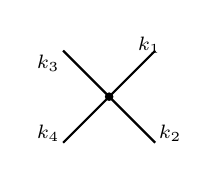
\begin{tikzpicture}[baseline=-0.45ex,scale=0.78]
  \draw[line width=0.8pt] (-0.75,0.75) -- (0,0) -- (-0.75,-0.75);
  \draw[line width=0.8pt] (0,0) -- (0.75,0.75);
  \draw[line width=0.8pt] (0,0) -- (0.75,-0.75);
  \fill (0,0) circle (2pt);
  \node[above] at (0.65,0.55) {\scriptsize \(k_1\)};
  \node[right] at (0.65,-0.6) {\scriptsize \(k_2\)};
  \node[left] at (-0.65,0.55) {\scriptsize \(k_3\)};
  \node[left] at (-0.65,-0.6) {\scriptsize \(k_4\)};
\end{tikzpicture}
\qquad
\ii\mathcal A
\]
is a function of
\[
  s=-(k_1+k_2)^2,
  \qquad
  t=-(k_1-k_3)^2.
\]
If a pair of \(\phi\)-particles form bound states, the latter should show
up as poles of \(\mathcal A\) at \(s<4m^2\).

The perturbative expansion begins as
\[
\begin{tikzpicture}[>=Stealth,baseline=-0.45ex,scale=0.72,
  dot/.style={fill,circle,inner sep=1.8pt}]
  \node at (-0.6,0) {\(\ii\mathcal A=\left[\right.\)};
  \begin{scope}[xshift=0.15cm]
    \draw (-0.45,0.45) -- (0,0) -- (-0.45,-0.45);
    \draw (0,0) -- (0.45,0.45);
    \draw (0,0) -- (0.45,-0.45);
    \fill (0,0) circle (1.8pt);
    \node[blue] at (0,0.82) {\scriptsize \(-\ii g\)};
  \end{scope}
  \node at (1.1,0) {\(+\)};
  \begin{scope}[xshift=1.85cm]
    \draw (-0.65,0.55) -- (-0.15,0.12);
    \draw (-0.65,-0.55) -- (-0.15,-0.12);
    \draw (0.15,0.12) -- (0.65,0.55);
    \draw (0.15,-0.12) -- (0.65,-0.55);
    \draw (0,0) circle (0.2);
    \fill (-0.15,0) circle (1.6pt);
    \fill (0.15,0) circle (1.6pt);
  \end{scope}
  \node at (3.0,0) {\(+\)};
  \begin{scope}[xshift=3.75cm]
    \draw (-0.45,0.45) -- (0,0.15) -- (0.45,0.45);
    \draw (-0.45,-0.45) -- (0,-0.15) -- (0.45,-0.45);
    \draw (0,0.15) arc (90:-90:0.15);
    \draw (0,-0.15) arc (-90:-270:0.15);
    \fill (0,0.15) circle (1.5pt);
    \fill (0,-0.15) circle (1.5pt);
  \end{scope}
  \node at (4.85,0) {\(+\)};
  \begin{scope}[xshift=5.55cm]
    \draw (-0.45,0.45) -- (0,0.15) -- (0.45,0.45);
    \draw (-0.45,-0.45) -- (0,-0.15) -- (0.45,-0.45);
    \draw (0,0.15) arc (90:-90:0.15);
    \draw (0,-0.15) arc (-90:-270:0.15);
    \draw (-0.10,0.25) .. controls (0.05,0.58) and (0.32,0.58) .. (0.47,0.25);
    \fill (0,0.15) circle (1.5pt);
    \fill (0,-0.15) circle (1.5pt);
  \end{scope}
  \node at (6.55,0) {\(+\cdots\left.\right]\)};
  \node at (8.05,0) {\(\times\left(Z_\phi^{1/2}\right)^4\)};
\end{tikzpicture}
\]
The external factors do not affect the position of the poles in \(s\).
The one-loop \(s\)-channel bubble is
\[
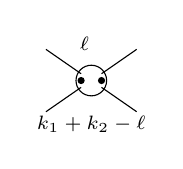
\begin{tikzpicture}[baseline=-0.55ex,scale=0.72]
  \draw (-0.8,0.55) -- (-0.18,0.12);
  \draw (-0.8,-0.55) -- (-0.18,-0.12);
  \draw (0.18,0.12) -- (0.8,0.55);
  \draw (0.18,-0.12) -- (0.8,-0.55);
  \draw (0,0) circle (0.27);
  \fill (-0.18,0) circle (1.8pt);
  \fill (0.18,0) circle (1.8pt);
  \node[above] at (-0.12,0.36) {\scriptsize \(\ell\)};
  \node[below] at (0,-0.45) {\scriptsize \(k_1+k_2-\ell\)};
\end{tikzpicture}
=
\frac{(-\ii g)^2}{2}
\int \frac{\dd^D\ell}{(2\pi)^D}\,
\frac{-\ii}{\ell^2+m^2-\ii\epsilon}\,
\frac{-\ii}{(k_1+k_2-\ell)^2+m^2-\ii\epsilon}.
\]
Using a Feynman parameter and Wick rotation,
\[
  =
  \frac{\ii g^2}{2}
  \int \frac{\dd^D\ell_E}{(2\pi)^D}
  \int_0^1\dd x\,
  \frac{1}{\left[\ell_E^2-sx(1-x)+m^2-\ii\epsilon\right]^2}.
\]
Specialize to the \(D=2\) case:
\[
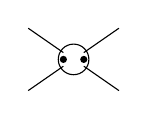
\begin{tikzpicture}[baseline=-0.55ex,scale=0.72]
  \draw (-0.8,0.55) -- (-0.18,0.12);
  \draw (-0.8,-0.55) -- (-0.18,-0.12);
  \draw (0.18,0.12) -- (0.8,0.55);
  \draw (0.18,-0.12) -- (0.8,-0.55);
  \draw (0,0) circle (0.27);
  \fill (-0.18,0) circle (1.8pt);
  \fill (0.18,0) circle (1.8pt);
\end{tikzpicture}
=
\frac{\ii g^2}{8\pi}
\int_0^1\dd x\,
\frac{1}{-sx(1-x)+m^2-\ii\epsilon}
\equiv
\frac{\ii g^2}{8\pi}f(s).
\]
Therefore the bubble chain gives
\[
  \ii\mathcal A
  =
  -\ii g
  \sum_{L=0}^\infty
  \left(-\frac{g}{8\pi}f(s)\right)^L
  =
  \frac{-\ii g}{1+\frac{g}{8\pi}f(s)}.
\]
For \(s\) approaching \(4m^2\) from below,
\[
  s=4m^2-\delta,\qquad \delta\to0^+,
\]
\[
  f(s)\simeq\frac{\pi}{m\sqrt{\delta}}.
\]
Thus \(\mathcal A\) acquires a pole if \(g<0\), at
\[
  \delta\simeq\left(\frac{g}{8m}\right)^2.
\]
Interpretation: for weak and negative coupling \(g\), there is a bound
state of mass
\[
  M\simeq 2m-\frac{g^2}{256m^3}.
\]
One might worry that \(\phi^4\) theory with negative \(g\) is
ill-defined nonperturbatively, because the scalar potential
\[
  V(\phi)=\frac12m^2\phi^2+\frac{g}{4!}\phi^4
\]
is not bounded from below, so that the perturbative vacuum is not the
true vacuum state.  Nonetheless, the same perturbative analysis applies
to scalar theories with additional \(\phi^6,\phi^8\) couplings, etc.;
for example
\[
  V(\phi)=\frac{m^2}{\beta^2}\cos(\beta\phi),
  \qquad
  \beta=\frac{\sqrt g}{m},
\]
the sine-Gordon model.

\subsection{Bethe--Salpeter Amplitudes}

More generally, we can probe the state \(\ket{B}\) of a composite
particle using
\[
  \bra{\Omega}T\hat\phi(x_1)\hat\phi(x_2)\ket{B}
  \equiv \Phi_B(x_1,x_2),
\]
the Bethe--Salpeter amplitude.

Similarly to the \(2\to2\) scattering amplitude, we can consider the
time-ordered four-point Green function
\[
\begin{aligned}
  \widetilde G(k_1,\ldots,k_4)
  &=
  \int \dd^D x_1\cdots \dd^D x_4\,
  \exp\!\left[-\ii\sum_{j=1}^4 k_j\cdot x_j\right]
\\
  &\qquad\qquad\times
  \bra{\Omega}T\hat\phi(x_1)\cdots\hat\phi(x_4)\ket{\Omega}.
\end{aligned}
\]
Diagrammatically,
\[
\begin{tikzpicture}[baseline=-0.45ex,scale=0.82,
  leg/.style={line width=0.8pt},
  blob/.style={draw,circle,fill=gray!20,pattern=north east lines,
    pattern color=gray!70,minimum size=0.9cm,inner sep=0pt}]
  \node[blob] (b) at (0,0) {};
  \draw[leg] (-1.0,0.72) -- (b.140);
  \draw[leg] (-1.0,-0.72) -- (b.220);
  \draw[leg] (b.40) -- (1.0,0.72);
  \draw[leg] (b.320) -- (1.0,-0.72);
  \fill (-1.0,0.72) circle (1.8pt);
  \fill (-1.0,-0.72) circle (1.8pt);
  \fill (1.0,0.72) circle (1.8pt);
  \fill (1.0,-0.72) circle (1.8pt);
\end{tikzpicture}
\]
The existence of a bound state \(\ket{B}\) of invariant mass \(M\)
gives rise to a pole of \(\widetilde G\) at
\[
  (k_1+k_2)^2=-M^2,
\]
by the same derivation as the Källén--Lehmann spectral representation of
the time-ordered two-point function.

Let
\[
  k_1+k_2\to k_B,
  \qquad
  k_B^0=\sqrt{\vec k_B^{\,2}+M^2}.
\]
Near the bound-state pole,
\[
  \widetilde G
  \longrightarrow
  (2\pi)^D\delta^D(k_1+\cdots+k_4)\,
  \frac{-\ii}{(k_1+k_2)^2+M^2-\ii\epsilon}\,
  \widetilde\Phi_B(k_1,k_2)\,
  \widetilde\Phi_B^{\,*}(-k_3,-k_4).
\]
Here
\[
\begin{aligned}
  \Phi_B(x_1,x_2)
  &\equiv
  \bra{\Omega}T\hat\phi(x_1)\hat\phi(x_2)\ket{B,\vec k_B}
\\
  &=
  \int \frac{\dd^D k_1}{(2\pi)^D}
       \frac{\dd^D k_2}{(2\pi)^D}\,
  \ee^{\ii k_1\cdot x_1+\ii k_2\cdot x_2}\,
  (2\pi)^D\delta^D(k_1+k_2-k_B)\,
  \frac{\widetilde\Phi_B(k_1,k_2)}
       {(2\pi)^{(D-1)/2}\sqrt{2\omega_{k_B}}}.
\end{aligned}
\]

\begin{center}
\begin{tikzpicture}[>=Stealth,scale=0.9,
  leg/.style={line width=0.8pt},
  blob/.style={draw,circle,fill=gray!20,pattern=north east lines,
    pattern color=gray!70,minimum size=0.78cm,inner sep=0pt},
  bound/.style={violet,line width=1.8pt,postaction={
    decorate,decoration={markings,mark=at position 0.5 with {\arrow{Stealth}}}}}]
  \node[blob,label=below:{\(\Phi_B\)}] (l) at (0,0) {};
  \node[blob] (r) at (3.1,0) {};
  \draw[leg] (-0.95,0.65) -- (l.140);
  \draw[leg] (-0.95,-0.65) -- (l.220);
  \draw[leg] (r.40) -- (4.05,0.65);
  \draw[leg] (r.320) -- (4.05,-0.65);
  \draw[bound] (2.72,0) -- (0.39,0);
  \node[violet] at (1.55,-0.35) {\(B\)};
  \fill (-0.95,0.65) circle (1.8pt);
  \fill (-0.95,-0.65) circle (1.8pt);
  \fill (4.05,0.65) circle (1.8pt);
  \fill (4.05,-0.65) circle (1.8pt);
\end{tikzpicture}
\end{center}

In the ``two-particle approximation'', the bound-state pole comes from a
divergence in summing over diagrams of the type
\[
\begin{tikzpicture}[baseline=-0.5ex,scale=0.72,
  leg/.style={line width=0.75pt},
  blob/.style={draw,circle,fill=gray!20,pattern=north east lines,
    pattern color=gray!70,minimum size=0.75cm,inner sep=0pt},
  kernel/.style={draw,rounded corners=2pt,minimum width=0.55cm,
    minimum height=1.25cm,inner sep=0pt,line width=0.75pt}]
  \node[blob] (b) at (0,0) {};
  \draw[leg] (-0.9,0.62) -- (b.140);
  \draw[leg] (-0.9,-0.62) -- (b.220);
  \draw[leg] (b.40) -- (0.9,0.62);
  \draw[leg] (b.320) -- (0.9,-0.62);
  \node at (1.55,0) {\(\supset\)};
  \draw[leg] (2.15,0.4) -- (2.85,0.4);
  \draw[leg] (2.15,-0.4) -- (2.85,-0.4);
  \fill (2.5,0.4) circle (1.7pt);
  \fill (2.5,-0.4) circle (1.7pt);
  \node at (3.35,0) {\(+\)};
  \node[kernel] (k1) at (4.4,0) {};
  \draw[leg] (3.45,0.42) -- (k1.west|-0,0.42);
  \draw[leg] (3.45,-0.42) -- (k1.west|-0,-0.42);
  \draw[leg] (k1.east|-0,0.42) -- (5.35,0.42);
  \draw[leg] (k1.east|-0,-0.42) -- (5.35,-0.42);
  \fill (3.45,0.42) circle (1.7pt);
  \fill (3.45,-0.42) circle (1.7pt);
  \fill (5.35,0.42) circle (1.7pt);
  \fill (5.35,-0.42) circle (1.7pt);
  \node at (5.85,0) {\(+\)};
  \node[kernel] (k2) at (6.8,0) {};
  \node[kernel] (k3) at (7.65,0) {};
  \draw[leg] (6.0,0.42) -- (k2.west|-0,0.42);
  \draw[leg] (6.0,-0.42) -- (k2.west|-0,-0.42);
  \draw[leg] (k2.east|-0,0.42) -- (k3.west|-0,0.42);
  \draw[leg] (k2.east|-0,-0.42) -- (k3.west|-0,-0.42);
  \draw[leg] (k3.east|-0,0.42) -- (8.45,0.42);
  \draw[leg] (k3.east|-0,-0.42) -- (8.45,-0.42);
  \foreach \x/\y in {6.0/0.42,6.0/-0.42,8.45/0.42,8.45/-0.42}
    \fill (\x,\y) circle (1.6pt);
  \node at (8.9,0) {\(+\cdots\)};
\end{tikzpicture}
\]
where \(\Pi\) contains no two-particle cuts.

\begin{center}
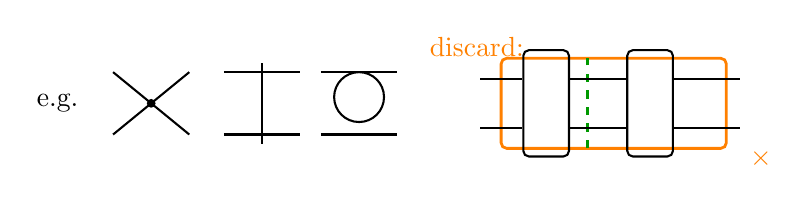
\begin{tikzpicture}[scale=0.88,
  leg/.style={line width=0.75pt},
  kernel/.style={draw,rounded corners=2pt,minimum width=0.58cm,
    minimum height=1.35cm,inner sep=0pt,line width=0.75pt}]
  \node at (-2.8,0) {e.g.};
  \begin{scope}[xshift=-1.45cm]
    \draw[leg] (-0.55,0.45) -- (0,0) -- (-0.55,-0.45);
    \draw[leg] (0,0) -- (0.55,0.45);
    \draw[leg] (0,0) -- (0.55,-0.45);
    \fill (0,0) circle (1.8pt);
  \end{scope}
  \begin{scope}[xshift=0.15cm]
    \draw[leg] (-0.55,0.45) -- (0.55,0.45);
    \draw[leg] (-0.55,-0.45) -- (0.55,-0.45);
    \draw[leg,line width=1.0pt] (0,-0.58) -- (0,0.58);
  \end{scope}
  \begin{scope}[xshift=1.55cm]
    \draw[leg] (-0.55,0.45) -- (0.55,0.45);
    \draw[leg] (-0.55,-0.45) -- (0.55,-0.45);
    \draw[leg] (0,0.45) arc (90:-270:0.36);
  \end{scope}
  \node[green!60!black] at (2.45,0) {\(\checkmark\)};
  \begin{scope}[xshift=4.6cm]
    \node[orange] at (-1.35,0.82) {discard:};
    \draw[orange,line width=1pt,rounded corners=2pt] (-1.0,-0.65) rectangle (2.25,0.65);
    \draw[green!60!black,dashed,line width=0.9pt] (0.25,-0.65) -- (0.25,0.65);
    \node[kernel] (a) at (-0.35,0) {};
    \node[kernel] (b) at (1.15,0) {};
    \draw[leg] (-1.3,0.35) -- (a.west|-0,0.35);
    \draw[leg] (-1.3,-0.35) -- (a.west|-0,-0.35);
    \draw[leg] (a.east|-0,0.35) -- (b.west|-0,0.35);
    \draw[leg] (a.east|-0,-0.35) -- (b.west|-0,-0.35);
    \draw[leg] (b.east|-0,0.35) -- (2.45,0.35);
    \draw[leg] (b.east|-0,-0.35) -- (2.45,-0.35);
    \node[orange] at (2.75,-0.8) {\(\times\)};
  \end{scope}
\end{tikzpicture}
\end{center}

The sum obeys the recursive relation
\[
\begin{tikzpicture}[baseline=-0.5ex,scale=0.72,
  leg/.style={line width=0.75pt},
  blob/.style={draw,rounded corners=2pt,fill=gray!20,pattern=north east lines,
    pattern color=gray!70,minimum width=0.62cm,minimum height=1.32cm,inner sep=0pt},
  kernel/.style={draw,rounded corners=2pt,minimum width=0.56cm,
    minimum height=1.25cm,inner sep=0pt,line width=0.75pt}]
  \node[blob,label=below:{\(\widehat\Gamma\)}] (g) at (0,0) {};
  \draw[leg] (-0.95,0.4) -- (g.west|-0,0.4);
  \draw[leg] (-0.95,-0.4) -- (g.west|-0,-0.4);
  \draw[leg] (g.east|-0,0.4) -- (0.95,0.4);
  \draw[leg] (g.east|-0,-0.4) -- (0.95,-0.4);
  \node at (1.55,0) {\(=\)};
  \node[kernel,label=below:{\(\widehat V\)}] (v) at (2.35,0) {};
  \draw[leg] (1.55,0.4) -- (v.west|-0,0.4);
  \draw[leg] (1.55,-0.4) -- (v.west|-0,-0.4);
  \draw[leg] (v.east|-0,0.4) -- (3.2,0.4);
  \draw[leg] (v.east|-0,-0.4) -- (3.2,-0.4);
  \node at (3.65,0) {\(+\)};
  \node[kernel] (v2) at (4.55,0) {};
  \node[blob] (g2) at (5.65,0) {};
  \draw[leg] (3.85,0.4) -- (v2.west|-0,0.4);
  \draw[leg] (3.85,-0.4) -- (v2.west|-0,-0.4);
  \draw[leg] (v2.east|-0,0.4) -- (g2.west|-0,0.4);
  \draw[leg] (v2.east|-0,-0.4) -- (g2.west|-0,-0.4);
  \draw[leg] (g2.east|-0,0.4) -- (6.45,0.4);
  \draw[leg] (g2.east|-0,-0.4) -- (6.45,-0.4);
\end{tikzpicture}
\]
or, equivalently,
\[
  (1-\widehat V)\widehat\Gamma=\widehat V .
\]
The residue of \(\widehat\Gamma\) at the bound-state pole
\(P^2=-M^2\) is proportional to \(\widetilde\Phi_B\), which obeys
\[
  (1-\widehat V)\widetilde\Phi_B=0.
\]
Diagrammatically,
\[
\begin{tikzpicture}[baseline=-0.55ex,scale=0.78,
  leg/.style={line width=0.75pt},
  blob/.style={draw,circle,fill=gray!20,pattern=north east lines,
    pattern color=gray!70,minimum size=0.78cm,inner sep=0pt},
  kernel/.style={draw,rounded corners=2pt,minimum width=0.58cm,
    minimum height=1.35cm,inner sep=0pt,line width=0.75pt},
  bound/.style={violet,line width=1.7pt,postaction={
    decorate,decoration={markings,mark=at position 0.5 with {\arrow{Stealth}}}}}]
  \node[blob,label=below:{\(\widetilde\Phi_B\)}] (phi) at (0,0) {};
  \draw[leg] (-0.95,0.65) -- (phi.140);
  \draw[leg] (-0.95,-0.65) -- (phi.220);
  \draw[bound] (phi.east) -- (1.15,0);
  \node at (1.7,0) {\(=\)};
  \node[kernel] (v) at (2.55,0) {};
  \node[blob,label=below:{\(\widetilde\Phi_B\)}] (phi2) at (3.8,0) {};
  \draw[leg] (1.85,0.42) -- (v.west|-0,0.42);
  \draw[leg] (1.85,-0.42) -- (v.west|-0,-0.42);
  \draw[leg] (v.east|-0,0.42) -- (phi2.west|-0,0.28);
  \draw[leg] (v.east|-0,-0.42) -- (phi2.west|-0,-0.28);
  \draw[bound] (phi2.east) -- (4.8,0);
  \draw[blue,dashed,line width=0.9pt] (3.25,-0.85) rectangle (5.05,0.85);
\end{tikzpicture}
\]
Equivalently, in terms of the amputated Bethe--Salpeter amplitude
\(\Psi_B\),
\[
\begin{tikzpicture}[baseline=-0.55ex,scale=0.78,
  leg/.style={line width=0.75pt},
  blob/.style={draw,circle,fill=gray!20,pattern=north east lines,
    pattern color=gray!70,minimum size=0.78cm,inner sep=0pt},
  kernel/.style={draw,rounded corners=2pt,minimum width=0.58cm,
    minimum height=1.35cm,inner sep=0pt,line width=0.75pt},
  bound/.style={violet,line width=1.7pt,postaction={
    decorate,decoration={markings,mark=at position 0.5 with {\arrow{Stealth}}}}},
  amp/.style={green!60!black,line width=1.0pt}]
  \node[blob,label=below:{\(\Psi_B\)}] (psi) at (0,0) {};
  \draw[leg] (-0.95,0.65) -- (psi.140);
  \draw[leg] (-0.95,-0.65) -- (psi.220);
  \draw[amp] (-0.95,0.5) -- (-0.73,0.78);
  \draw[amp] (-0.95,-0.5) -- (-0.73,-0.78);
  \draw[bound] (psi.east) -- (1.0,0);
  \node at (1.55,0) {\(=\)};
  \node[kernel] (v) at (2.35,0) {};
  \node[blob,label=below:{\(\Psi_B\)}] (psi2) at (3.65,0) {};
  \draw[leg] (1.75,0.42) -- (v.west|-0,0.42);
  \draw[leg] (1.75,-0.42) -- (v.west|-0,-0.42);
  \draw[leg] (v.east|-0,0.42) -- (psi2.west|-0,0.28);
  \draw[leg] (v.east|-0,-0.42) -- (psi2.west|-0,-0.28);
  \draw[amp] (1.75,0.2) -- (1.95,0.6);
  \draw[amp] (1.75,-0.2) -- (1.95,-0.6);
  \draw[bound] (psi2.east) -- (4.6,0);
  \draw[blue,dashed,line width=0.9pt] (3.05,-0.85) rectangle (4.85,0.85);
\end{tikzpicture}
\]
This is the Bethe--Salpeter equation.

\subsection{Analyticity, Crossing, and Landau Singularities}

General expectations on the analyticity properties of scattering
amplitudes begin with the \(2\to2\) amplitude of identical, massive
scalar particles,
\[
  \mathcal A(s,t).
\]
In the center-of-mass frame,
\[
  s=E^2=4(k^2+m^2),
  \qquad
  t=-2k^2(1-\cos\theta).
\]
The amplitude can be analytically continued away from the physical
region
\[
  s,t\in\mathbb R,\qquad s\geq4m^2-t,\qquad t\leq0,
\]
with
\[
  u=4m^2-s-t\leq0.
\]
We still denote the result of analytic continuation by
\(\mathcal A(s,t)\).

\begin{center}
\begin{tikzpicture}[>=Stealth,scale=0.9]
  \begin{scope}
    \node[draw,circle,fill=gray!18,pattern=north east lines,
      pattern color=gray!70,minimum size=0.78cm,inner sep=0pt] (b) at (0,0) {};
    \draw[line width=0.85pt] (-1.0,0.65) -- (b.140);
    \draw[line width=0.85pt] (-1.0,-0.65) -- (b.220);
    \draw[line width=0.85pt] (b.40) -- (1.0,0.65);
    \draw[line width=0.85pt] (b.320) -- (1.0,-0.65);
    \node[below] at (0,-1.05) {\(\mathcal A(s,t)\)};
  \end{scope}
  \begin{scope}[xshift=4.1cm]
    \draw[->,gray,line width=1pt] (-1.25,0) -- (-0.25,0);
    \draw[->,gray,line width=1pt] (1.25,0) -- (0.25,0);
    \draw[->,gray,line width=1pt] (0,0) -- (0.9,0.7);
    \draw[->,gray,line width=1pt] (0,0) -- (-0.55,-0.95);
    \draw[gray,line width=0.8pt] (0.45,0.1) arc (12:48:0.9);
    \node[gray] at (0.78,0.38) {\(\theta\)};
    \node[gray] at (1.1,0.85) {\(k\)};
    \node[gray] at (1.42,-0.05) {\(k\)};
    \node[align=left] at (0,-1.05)
      {\(s=E^2=4(k^2+m^2)\)\\
       \(t=-2k^2(1-\cos\theta)\)};
  \end{scope}
\end{tikzpicture}
\end{center}

Fix \(t<0\).  In the complex \(s\)-plane the physical amplitude is
\[
  \lim_{\epsilon\to0^+}\mathcal A(s+\ii\epsilon,t).
\]
The first sheet has an \(s\)-channel cut starting at \(4m^2\), a
\(u\)-channel cut starting at \(-t\), and possible bound-state poles.

\begin{center}
\begin{tikzpicture}[>=Stealth,scale=0.95]
  \draw[black,line width=0.7pt] (-3.7,-1.75) rectangle (4.15,1.9);
  \node[anchor=west] at (-3.45,1.55) {cplx \(s\)-plane};
  \draw[->,line width=0.75pt] (-3.45,0) -- (3.85,0);
  \draw[->,line width=0.75pt] (0,-1.5) -- (0,1.55);
  \node[below] at (0,0) {\(0\)};
  \draw[orange,decorate,decoration={snake,amplitude=0.55mm,segment length=2.8mm},
    line width=1pt] (-3.25,0) -- (-1.6,0);
  \node[orange,align=center] at (-2.65,-0.48) {\(u\)-channel\\cut};
  \node[below] at (-1.6,0) {\(-t\)};
  \fill[gray] (-0.95,0.22) circle (2pt);
  \fill[gray] (-0.45,0.22) circle (2pt);
  \node[gray,align=center] at (-0.7,0.72) {possible\\bound-state poles};
  \draw[red,decorate,decoration={snake,amplitude=0.55mm,segment length=2.8mm},
    line width=1pt] (1.2,0) -- (3.65,0);
  \node[below] at (1.2,0) {\(4m^2\)};
  \node[red,align=center] at (2.78,-0.48) {\(s\)-channel\\cut};
  \draw[blue,line width=1.2pt,->]
    (1.25,0.62) .. controls (1.85,1.25) and (2.65,1.15) .. (2.98,0.15);
  \node[blue] at (2.35,0.95) {physical};
  \node[blue] at (3.35,0.55) {phys};
\end{tikzpicture}
\end{center}

The analytically continued \(\mathcal A(s,t)\) is expected to obey:
\begin{itemize}
\item Real analyticity,
\[
  \mathcal A(s^*,t^*)=\bigl(\mathcal A(s,t)\bigr)^* .
\]
In perturbation theory this follows from reality of the coupling
constants in the Lagrangian.
\item Crossing, superficially a consequence of LSZ and symmetry of Green
functions.
\end{itemize}

On the real \((s,t)\)-plane, the \(s\)-, \(t\)-, and \(u\)-channel
physical regions are related by analytic continuation.

\begin{center}
\begin{tikzpicture}[>=Stealth,scale=0.82]
  \draw[->,line width=0.75pt] (-3.1,0) -- (3.35,0) node[right] {\(s\)};
  \draw[->,line width=0.75pt] (0,-2.5) -- (0,2.8) node[above] {\(t\)};
  \node[below] at (1.45,0) {\(4m^2\)};
  \node[left] at (0,1.35) {\(4m^2\)};
  \node[below] at (-1.45,0) {\(-4m^2\)};
  \draw[blue,line width=1.5pt] (1.45,0) -- (3.0,0.95);
  \node[blue,align=center,fill=white,inner sep=1pt] at (2.25,-0.55)
    {physical region\\\(s\)-channel};
  \draw[orange,line width=1.5pt] (-1.45,0) -- (-3.0,0.95);
  \node[orange,align=center,fill=white,inner sep=1pt] at (-2.2,-0.55)
    {\(u\)-channel};
  \draw[green!55!black,line width=1.5pt] (0,1.45) -- (-0.95,2.55);
  \node[green!55!black,anchor=west] at (0.55,2.35) {\(t\)-channel};
  \draw[purple,line width=1.1pt,->]
    (2.2,0.65) .. controls (0.6,1.65) and (-1.0,1.65) .. (-2.2,0.65);
  \node[purple,align=center,fill=white,inner sep=1pt] at (0.15,1.05)
    {related by analytic\\continuation};
  \node at (-2.85,1.15) {\(24\)};
  \node at (2.85,1.15) {\(13\)};
  \node at (-1.15,2.45) {\(14\)};
\end{tikzpicture}
\end{center}

Unitarity gives, for the partial-wave decomposition,
\[
  \mathcal A(s,t)
  =
  -16\pi\ii
  \sqrt{\frac{s}{s-4m^2}}\,
  \sum_{\ell=0}^{\infty}
  (2\ell+1)P_\ell(\cos\theta)\bigl(S_\ell(s)-1\bigr),
\]
and
\[
  |S_\ell(s)|\leq1\qquad\text{for }s\geq4m^2.
\]
Also,
\[
  |S_\ell(s)|=1
  \qquad\text{for }4m^2\leq s\leq M_{\mathrm{inel}}^2,
\]
where \(M_{\mathrm{inel}}\) is the threshold of inelastic processes.

Caution: not all singularities of \(\mathcal A\) on the first sheet have
the interpretation of an intermediate physical state, either a bound
state or a multi-particle scattering state.  Such singularities are
called anomalous thresholds.

Consider a loop integral of the schematic form
\[
  \int \dd^D k\,
  \frac{(\cdots)}
  {\prod_{i=1}^N\bigl(k_i^2+m_i^2-\ii\epsilon\bigr)},
  \qquad
  k_i=k+\text{external momenta},
\]
where the numerator is polynomial in the \(k_i\)'s.  Feynman
parametrization gives
\[
  \int \dd^D k
  \int_0^1\prod_{i=1}^N\dd\alpha_i\,
  \delta\!\left(\sum_{i=1}^N\alpha_i-1\right)
  \frac{(\cdots)}
  {\left[
    \sum_{i=1}^N\alpha_i(k_i^2+m_i^2)-\ii\epsilon
  \right]^N}.
\]
As a function of external momenta, this can be analytically continued so
long as the poles of the integrand stay away from the integration
contour.  Even if a pole hits the integration contour, the
\(\alpha_i\) or \(k^\mu\) contour can generically be deformed to evade
the pole.

A singularity can occur only if the contour cannot be deformed away from
the pole.
\[
\begin{tikzpicture}[baseline=-0.55ex,scale=0.86,>=Stealth]
  \draw[blue,line width=1.2pt,->]
    (-1.7,-0.95) .. controls (-1.2,0.25) and (-0.2,0.7) .. (1.6,0.88);
  \fill[red] (-0.2,0.55) circle (2pt) node[above] {\(x_0\)};
  \fill[orange] (-0.28,0.35) circle (2pt) node[left] {\(x\)};
  \draw[orange,->,line width=1pt] (-0.28,0.8) -- (-0.28,0.43);
  \draw[orange,->,line width=1pt] (-0.28,0.05) -- (-0.28,0.28);
\end{tikzpicture}
\]
This happens when all derivatives of the denominator with respect to
\(\alpha_i\) and \(k^\mu\) vanish.  Equivalently,
\[
\left\{
\begin{aligned}
  k_i^2+m_i^2&=0,\qquad i=1,\ldots,N,\\
  \frac{\partial}{\partial k^\mu}
  \sum_{i=1}^N \alpha_i(k_i^2+m_i^2)&=0.
\end{aligned}
\right.
\]
These are the Landau equations; the second equation is
\[
  2\sum_i\alpha_i k_{i\mu}=0.
\]

On the first Riemann sheet, also called the physical sheet and not to be
confused with the physical region, singularities of the amplitude occur
at solutions to the Landau equations with \(\alpha_i>0\).  For more
details, see Eden et al., \emph{The Analytic S-Matrix} (1966).

For example, take a two-particle loop with
\[
  k_2=k+p.
\]
The singularity occurs when
\[
  k^2+m^2=0=(k+p)^2+m^2,
  \qquad
  \alpha(k+p)+(1-\alpha)k=0
\]
for some \(0\leq\alpha\leq1\).  This gives
\[
  \alpha=\frac12,\qquad k=-\frac p2,\qquad p^2=-4m^2.
\]
This is the two-particle threshold.

\begin{center}
\begin{tikzpicture}[>=Stealth,scale=0.88]
  \begin{scope}
    \draw[line width=0.8pt] (-1.4,0.45) -- (-0.45,0.45);
    \draw[line width=0.8pt] (-1.4,-0.45) -- (-0.45,-0.45);
    \draw[line width=0.8pt] (1.4,0.45) -- (0.45,0.45);
    \draw[line width=0.8pt] (1.4,-0.45) -- (0.45,-0.45);
    \draw[line width=0.8pt] (0,0) ellipse (0.55 and 0.48);
    \node[blue] at (-1.55,0) {\(p\)};
    \node[blue] at (1.55,0) {\(p\)};
    \node[blue] at (0,-0.75) {\(k_1=k\)};
    \node[blue] at (0,0.78) {\(k_2=k+p\)};
  \end{scope}
  \begin{scope}[xshift=4.2cm]
    \draw[->,line width=1.0pt] (0,0) -- (-1.1,0) node[left] {\(k_1\)};
    \draw[->,line width=1.0pt] (0,0) -- (1.1,0) node[right] {\(k_2\)};
    \draw[blue,->,line width=1pt] (1.1,-0.22) -- (-1.1,-0.22)
      node[midway,below] {\(P\)};
    \draw[decorate,decoration={brace,amplitude=4pt},gray]
      (-1.1,0.18) -- (0,0.18) node[midway,above=4pt] {\(m_1\)};
    \draw[decorate,decoration={brace,amplitude=4pt},gray]
      (0,0.18) -- (1.1,0.18) node[midway,above=4pt] {\(m_2\)};
    \node[blue] at (0,-0.75) {\(-P^2=(m_1+m_2)^2\)};
  \end{scope}
\end{tikzpicture}
\end{center}

A pictorial way to see the singularity is to think of
\((k^0,\ii\vec k)\) as a vector of length \(m\).  With
\[
  \alpha_1 k_1+\alpha_2 k_2=0,\qquad
  0<\alpha_1,\alpha_2<1,
\]
one obtains the threshold condition above.

Now consider a triangle diagram.  A singularity occurs on the first
sheet if the corresponding on-shell vectors can be arranged.

\begin{center}
\begin{tikzpicture}[>=Stealth,scale=0.82]
  \coordinate (a) at (-1.25,0.25);
  \coordinate (b) at (1.0,0.75);
  \coordinate (c) at (0.55,-1.05);
  \draw[line width=0.9pt] (a) -- (b) -- (c) -- cycle;
  \foreach \p in {a,b,c} \fill[white,draw,line width=0.75pt] (\p) circle (0.16);
  \draw[blue,->,line width=1pt] (-2.2,0.25) -- (a) node[left] {\(P_1\)};
  \draw[blue,->,line width=1pt] (1.65,1.35) -- (b) node[right] {\(P_3\)};
  \draw[blue,->,line width=1pt] (0.65,-2.0) -- (c) node[below] {\(P_2\)};
  \node[blue] at (-0.25,0.72) {\(k_3\)};
  \node[blue] at (1.0,-0.1) {\(k_2\)};
  \node[blue] at (-0.45,-0.62) {\(k_1\)};
  \node[align=center] at (4.4,1.25) {singularity occurs on\\the first sheet if};
  \begin{scope}[xshift=4.35cm,yshift=-0.95cm]
    \draw[blue,->,line width=1pt] (0,0) -- (-1.0,-1.0) node[left] {\(P_2\)};
    \draw[blue,->,line width=1pt] (0,0) -- (1.15,-0.85) node[right] {\(P_1\)};
    \draw[blue,->,line width=1pt] (-1.0,-1.0) -- (1.15,-0.85)
      node[midway,below] {\(P_3\)};
    \draw[->,line width=1pt] (0,0) -- (0.1,1.2) node[above] {\(k_1\)};
    \node[gray] at (0.35,0.55) {\(m\)};
    \node[gray] at (-0.63,-0.62) {\(m_2\)};
    \node[gray] at (0.65,-0.75) {\(m_3\)};
  \end{scope}
\end{tikzpicture}
\end{center}

Take
\[
  P_3^2=-M_3^2
\]
and similarly \(P_1^2=-M_1^2\), \(P_2^2=-M_2^2\).  If
\[
  M_1,M_2<\sqrt2\,m,
\]
the required vectors can only be arranged in a way that fails the Landau
equation, so the amplitude is nonsingular.

\begin{center}
\begin{tikzpicture}[>=Stealth,scale=0.9]
  \draw[->,line width=1pt] (0,0) -- (1.45,0) node[right] {\(k_1\)};
  \draw[->,line width=1pt] (0,0) -- (0.9,1.25) node[above] {\(k_2\)};
  \draw[->,line width=1pt] (0,0) -- (0.95,-1.25) node[below] {\(k_3\)};
  \draw[blue,->,line width=1pt] (1.45,0) -- (0.9,1.25) node[midway,right] {\(M_2\)};
  \draw[blue,->,line width=1pt] (0.95,-1.25) -- (1.45,0) node[midway,right] {\(M_1\)};
  \node[anchor=west] at (2.45,0.25) {cannot satisfy the Landau equation};
  \node[anchor=west] at (2.45,-0.45) {\(\Longrightarrow\) amplitude nonsingular.};
\end{tikzpicture}
\end{center}

On the other hand, if
\[
  M_1,M_2>\sqrt2\,m,
\]
the vectors can be arranged.  Then the amplitude acquires a Landau
singularity at a specific value
\[
  P_3^2=-M_3^2,
\]
where \(M_3\) is determined by \(M_1,M_2,m\).  This singularity does not
admit the interpretation of a bound state.

\begin{center}
\begin{tikzpicture}[>=Stealth,scale=0.9]
  \draw[->,line width=1pt] (0,0) -- (1.3,0) node[right] {\(k_1\)};
  \draw[->,line width=1pt] (0,0) -- (0.75,1.05) node[above] {\(k_2\)};
  \draw[->,line width=1pt] (0,0) -- (0.75,-1.05) node[below] {\(k_3\)};
  \draw[blue,->,line width=1pt] (0.75,1.05) -- (1.55,0.35) node[right] {\(M_2\)};
  \draw[blue,->,line width=1pt] (0.75,-1.05) -- (1.55,-0.35) node[right] {\(M_1\)};
  \draw[blue,<->,line width=1pt] (0.25,-1.05) -- (0.25,1.05) node[midway,left] {\(M_3\)};
  \node[anchor=west] at (2.55,0.35) {\(\Longrightarrow\) Landau singularity};
  \node[anchor=west] at (2.55,-0.35) {at a specific value of \(P_3^2=-M_3^2\).};
\end{tikzpicture}
\end{center}

This anomalous-threshold singularity occurs in the sine-Gordon model
\[
  \text{[Coleman, Thun 1978]}.
\]
Working hypothesis: the kind of analytic structure of scattering
amplitudes found in perturbation theory also applies to the
nonperturbative amplitude, provided that we interpret the on-shell
internal propagators that give rise to Landau singularities as those of
actual particles.

Only a small subset of such analyticity assumptions have been rigorously
established based on robust axioms.

\paragraph{Some consequences of analyticity, crossing, and partial-wave
unitarity.}
For \(2\to2\) scattering of the lightest particles, write
\[
  x\equiv \cos\theta = 1+\frac{2t}{s-4m^2}.
\]
Fixing a physical value of \(s\), with \(s>4m^2\), let us inspect
\(\mathcal A(s,t)\) viewed as an analytic function of \(x\), denoted by
\(\mathcal A(x)\).

\begin{center}
\begin{tikzpicture}[>=Stealth,scale=0.84]
  \draw[line width=0.75pt] (-4.0,-2.0) rectangle (4.0,2.0);
  \node[anchor=west] at (-3.8,1.72) {cplx \(x\)-plane};
  \draw[->,line width=0.75pt] (-3.55,0) -- (3.55,0);
  \draw[blue,line width=1.4pt] (-0.9,0) -- (0.9,0);
  \fill[blue] (-0.9,0) circle (2pt) node[below] {\(-1\)};
  \fill[blue] (0.9,0) circle (2pt) node[below] {\(1\)};
  \node[blue] at (0,-0.45) {phys};
  \draw[purple,line width=1.2pt,dashed] (0,0) ellipse (1.72 and 0.93);
  \node[cyan!70!black] at (0,1.2) {Lehmann ellipse};
  \draw[red,decorate,decoration={snake,amplitude=0.55mm,segment length=2.6mm},
    line width=1pt] (-3.55,0) -- (-2.0,0);
  \draw[red,decorate,decoration={snake,amplitude=0.55mm,segment length=2.6mm},
    line width=1pt] (2.0,0) -- (3.55,0);
  \fill (-2.0,0) circle (2.2pt);
  \fill (2.0,0) circle (2.2pt);
  \node[red,align=center,font=\small] at (-3.25,-0.62) {\(u\)-channel\\cut};
  \node[red,align=center,font=\small] at (3.25,-0.62) {\(t\)-channel\\cut};
  \node[below,font=\small] at (-2.0,-0.22) {\(u=4m^2\)};
  \node[below,font=\small] at (2.0,-0.22) {\(t=4m^2\)};
  \fill[orange] (1.58,0) circle (2.2pt);
  \draw[orange,->,line width=1pt] (1.35,-1.25) -- (1.58,-0.12);
  \node[orange,align=center,font=\small] at (1.1,-1.55) {bound\\state pole};
  \node[gray,align=center,font=\footnotesize] at (2.75,-1.45)
    {\(x=\dfrac{s+4m^2}{s-4m^2}\)};
\end{tikzpicture}
\end{center}

The physical value of \(x\) lies between \(-1\) and \(1\) on the real
axis.  We expect \(\mathcal A(x)\) to be analytic on the complex
\(x\)-plane away from the \(t\)-channel branch cut
\[
  x\in \left[\frac{s+4m^2}{s-4m^2},\infty\right)
  \qquad\Longleftrightarrow\qquad
  t\in[4m^2,\infty),
\]
the \(u\)-channel cut
\[
  x\in
  \left(-\infty,-\frac{s+4m^2}{s-4m^2}\right],
\]
and possible poles that admit interpretation as bound states in the
\(t\)- and \(u\)-channels.

We can write
\[
  \mathcal A(x)
  =
  \oint_\gamma \frac{\dd z}{2\pi\ii}\,
  \frac{\mathcal A(z)}{z-x},
\]
provided that \(\gamma\) encircles \(x\) and \(\mathcal A(z)\) is
analytic inside of \(\gamma\).  Now use the identity
\[
  \frac{1}{z-x}
  =
  \sum_{\ell=0}^{\infty}
  (2\ell+1)P_\ell(x)Q_\ell(z),
\]
where \(Q_\ell\) is the Legendre function of the second kind.  The
identity holds when
\[
  \left|z+\sqrt{z^2-1}\right|
  >
  \left|x+\sqrt{x^2-1}\right|,
\]
with
\[
  Q_\ell(z)
  \equiv
  \frac12\int_{-1}^{1}\dd x\,
  \frac{P_\ell(x)}{z-x}
  =
  \int_{z+\sqrt{z^2-1}}^\infty
  \frac{\dd\xi}{\xi^{\ell+1}\sqrt{1-2\xi z+\xi^2}} .
\]
Indeed, at large \(\ell\),
\[
  P_\ell(x)\sim\left(x+\sqrt{x^2-1}\right)^\ell,
  \qquad
  Q_\ell(z)\sim\left(z+\sqrt{z^2-1}\right)^{-\ell}.
\]
The right-hand side of the identity converges when
\[
  \left|z+\sqrt{z^2-1}\right|
  >
  \left|x+\sqrt{x^2-1}\right|.
\]
Note that
\[
  \left\{z:\left|z+\sqrt{z^2-1}\right|=\text{const.}\right\}
\]
is an ellipse on the complex plane with foci \(\pm1\).  We will take
\(\gamma\) to be the largest ellipse with foci \(\pm1\) and encircling no
singularity of \(\mathcal A(z)\), for instance touching the first
\(t\)-channel bound-state pole.  This largest ellipse is called the
``Lehmann ellipse.''

Then
\[
\begin{aligned}
  \mathcal A(x)
  &=
  \oint_\gamma \frac{\dd z}{2\pi\ii}\,
  \sum_{\ell=0}^{\infty}
  (2\ell+1)P_\ell(x)Q_\ell(z)\mathcal A(z)  \\
  &=
  \sum_{\ell=0}^{\infty}
  (2\ell+1)P_\ell(x)
  \oint_\gamma \frac{\dd z}{2\pi\ii}\,
  Q_\ell(z)\mathcal A(z).
\end{aligned}
\]
The sum converges for \(x\) inside the Lehmann ellipse, so the
partial-wave expansion converges for unphysical \(x\), provided that
\(x\) lies inside the Lehmann ellipse.

\begin{center}
\begin{tikzpicture}[>=Stealth,scale=0.88]
  \draw[purple,dashed,line width=1.2pt] (0,0) ellipse (2.55 and 1.55);
  \draw[blue,line width=1.2pt] (-1,0) -- (1,0);
  \fill[blue] (-1,0) circle (2pt) node[above] {\(-1\)};
  \fill[blue] (1,0) circle (2pt) node[above] {\(1\)};
  \node[blue] at (0,-0.35) {phys};
  \draw[green!55!black,line width=1.2pt] (1,0) -- (2.1,0);
  \fill[orange] (2.1,0) circle (2.2pt);
  \node[green!55!black] at (2.2,-0.35) {\(x_0(s)\)};
  \draw[green!55!black,->,line width=1.1pt]
    (2.95,-1.25) .. controls (2.1,-1.2) and (1.75,-0.55) .. (2.05,-0.1);
  \node[green!55!black,align=center,anchor=west] at (3.05,-1.25)
    {\(1<x<x_0(s)\)\\[2pt]\(\Longleftrightarrow\)\\[2pt]\(0<t<t_0\)};
  \node[align=center] at (1.25,2.05)
    {for unphysical \(x\), provided that\\
    \(x\) lies inside the Lehmann ellipse};
\end{tikzpicture}
\end{center}

For real \(x\) inside the Lehmann ellipse,
\[
  \mathcal A(x)
  =
  -16\pi\ii
  \sqrt{\frac{s}{s-4m^2}}\,
  \sum_{\ell=0}^{\infty}
  (2\ell+1)P_\ell(x)\bigl(S_\ell(s)-1\bigr).
\]
Therefore
\[
  \Im\mathcal A(x)
  =
  16\pi
  \sqrt{\frac{s}{s-4m^2}}\,
  \sum_{\ell=0}^{\infty}
  (2\ell+1)P_\ell(x)\bigl(1-\Re S_\ell(s)\bigr),
\]
with \(0\leq 1-\Re S_\ell(s)\leq 2\).

Also recall the elastic and inelastic cross sections,
\[
  \sigma_{2\to2}
  =
  \frac{8\pi}{s-4m^2}
  \sum_{\ell=0}^{\infty}
  (2\ell+1)\left|S_\ell(s)-1\right|^2,
\]
\[
  \sigma_{\mathrm{inel}}
  =
  \frac{8\pi}{s-4m^2}
  \sum_{\ell=0}^{\infty}
  (2\ell+1)\left(1-\left|S_\ell(s)\right|^2\right).
\]
The total cross section is
\[
\begin{aligned}
  \sigma_{\mathrm{tot}}
  &=
  \sigma_{2\to2}+\sigma_{\mathrm{inel}} \\
  &=
  \frac{16\pi}{s-4m^2}
  \sum_{\ell=0}^{\infty}
  (2\ell+1)\bigl(1-\Re S_\ell(s)\bigr) \\
  &=
  \frac{1}{\sqrt{s(s-4m^2)}}\,\Im\mathcal A(x=1),
\end{aligned}
\]
the optical theorem.

Compare
\[
  \frac{1}{16\pi}
  \sqrt{\frac{s-4m^2}{s}}\,\Im\mathcal A(x)
  =
  \sum_{\ell=0}^{\infty}
  (2\ell+1)P_\ell(x)\bigl(1-\Re S_\ell(s)\bigr).
\]
Let
\[
  \frac{s-4m^2}{16\pi}\,\sigma_{\mathrm{tot}}
  =
  \sum_{\substack{\ell=0\\ \ell\ \mathrm{even}}}^{\infty}
  (2\ell+1)b_\ell
  \equiv \overline L^{\,2},
  \qquad
  \overline L
  =
  \sqrt{\frac{s-4m^2}{16\pi}\,\sigma_{\mathrm{tot}}}
  \simeq L,
\]
where \(L\) is an integer at high energies.

\begin{center}
\begin{tikzpicture}[>=Stealth,scale=0.82]
  \begin{scope}
    \draw[->] (0,0) -- (4.2,0) node[right] {\(\ell\)};
    \draw[->] (0,0) -- (0,2.15);
    \node[left] at (0,1.75) {\(2\)};
    \draw[purple,line width=1.2pt]
      (0.05,1.35) -- (0.45,1.35) -- (0.45,0.9) -- (0.85,0.9)
      -- (0.85,1.45) -- (1.35,1.45) -- (1.35,0.85) -- (1.8,0.85)
      -- (1.8,1.25) -- (2.35,1.25) -- (2.35,0.7) -- (2.9,0.7)
      -- (2.9,0.45) -- (3.45,0.45) -- (3.45,0.25);
    \node[purple] at (2.2,1.8) {\(1-\Re S_\ell\)};
  \end{scope}
  \begin{scope}[xshift=6.0cm]
    \draw[->] (0,0) -- (4.2,0) node[right] {\(\ell\)};
    \draw[->] (0,0) -- (0,2.15);
    \node[left] at (0,1.75) {\(2\)};
    \draw[blue,line width=1.2pt] (0,1.75) -- (3.05,1.75) -- (3.05,0);
    \draw[purple,dashed,line width=1pt] (3.05,0) -- (3.05,1.95);
    \node[blue] at (1.55,1.95) {\(b_\ell\)};
    \node[red,below] at (2.8,0) {\(L\)};
    \node[below] at (3.15,0) {\(L+2\)};
  \end{scope}
\end{tikzpicture}
\end{center}

The optical theorem gives
\[
  \sum_{\ell=0}^{\infty}(2\ell+1)\bigl(1-\Re S_\ell\bigr)
  =
  \sum_{\ell=0}^{\infty}(2\ell+1)b_\ell.
\]
For \(x>1\), \(P_\ell(x)\) increases with \(\ell\), and hence
\[
  \sum_{\ell=0}^{\infty}
  (2\ell+1)P_\ell(x)\bigl(1-\Re S_\ell\bigr)
  \geq
  \sum_{\ell=0}^{\infty}
  (2\ell+1)P_\ell(x)b_\ell.
\]
For \(x>1\),
\[
  P_\ell(x)
  =
  \frac{1}{\pi}\int_0^\pi
  \left(x+\cos\alpha\sqrt{x^2-1}\right)^\ell
  \dd\alpha
  >
  C_\delta
  \left[1+(1-\delta)\sqrt{x^2-1}\right]^\ell
\]
for all \(\ell\), given any arbitrarily small fixed \(\delta>0\) and
some constant \(C_\delta>0\).  Thus, putting
\[
  y=1+(1-\delta)\sqrt{x^2-1},
\]
one obtains
\[
  \Im\mathcal A(x)
  >
  \mathrm{const.}\,
  \sum_{\substack{\ell=0\\ \ell\ \mathrm{even}}}^{L}
  (2\ell+1)y^\ell
  \simeq
  \mathrm{const.}\,L\,\frac{y^L}{y-1}.
\]
For \(s\gg m^2\),
\[
  L\simeq
  \sqrt{\frac{s\,\sigma_{\mathrm{tot}}}{16\pi}},
  \qquad
  y-1\simeq(1-\delta)\sqrt{\frac{4t}{s}},
  \qquad
  y^L\simeq
  \exp\!\left[
    (1-\delta)\sqrt{\frac{t\,\sigma_{\mathrm{tot}}}{4\pi}}
  \right].
\]
Therefore
\[
  \Im\mathcal A(x)
  >
  \mathrm{const.}\,
  s\sqrt{\frac{\sigma_{\mathrm{tot}}}{t}}\,
  \exp\!\left[
    (1-\delta)\sqrt{\frac{t\,\sigma_{\mathrm{tot}}}{4\pi}}
  \right]
\]
for \(1<x<x_0(s)\), equivalently \(0<t<t_0\).

For \(x\simeq x_0(s)\), if \(\mathcal A(x)\) grows no faster than a
polynomial in \(s\) at large \(s\),
\[
  \Im\mathcal A(x)<C\,s^N
\]
for some \(N\), it then follows that
\[
  \sigma_{\mathrm{tot}}
  <
  \frac{(N-1)^2}{(1-\delta)^2}\,
  \frac{4\pi}{t_0}
  \left(\log\frac{s}{M^2}\right)^2,
  \qquad s\gg M^2.
\]
This is the Froissart--Martin bound, with \(M\) a mass scale.

\paragraph{Polynomial boundedness in complex energy.}
As a toy model, consider a linear scattering relation
\[
  f_{\mathrm{out}}(t)=
  \int \dd t'\,S(t-t')f_{\mathrm{in}}(t'),
  \qquad
  \widetilde S(\omega)=
  \int \dd t\,e^{i\omega t}S(t).
\]
Here \(\widetilde S(\omega)\) is the analogue of a scattering amplitude.
Causality says that \(S(t)\) is supported at \(t\geq 0\).  This implies
that \(\widetilde S(\omega)\) is analytic for \(\Im\omega>0\), and also
that there is no exponential growth as \(\omega\to\infty\) on the
upper-half complex plane.  Exponential growth as
\(\Im\omega\to\infty\) would correspond to a ``time advance.''

Let us now investigate the behavior of a \(2\to2\) amplitude
\(\mathcal A(s,t)\) at large complex \(s\).  For simplicity, assume
scattering of the lightest scalar particle, so there are no anomalous
thresholds, and assume there is no bound state, including no
self-coupling pole.

Fix real \(t<0\), and consider the analytic continuation of
\(\mathcal A(s,t)\) to the complex \(s\)-plane.
\[
  \mathcal A(s,t)=
  \oint_\gamma\frac{\dd s'}{2\pi i}\,
  \frac{\mathcal A(s',t)}{s'-s}.
\]

\begin{center}
\begin{tikzpicture}[scale=0.95,baseline=(current bounding box.center)]
  \draw[thick] (-4.6,-2.25) rectangle (4.6,2.35);
  \node[anchor=north west] at (-4.45,2.25) {complex \(s\)-plane};
  \draw[->] (-4.1,0) -- (4.15,0) node[right] {\(\Re s\)};
  \draw[->] (0,-1.9) -- (0,1.95) node[above] {\(\Im s\)};
  \draw[blue,line width=1pt,postaction={decorate},
    decoration={markings,mark=at position 0.35 with {\arrow{<}}}]
    (-3.95,0.18) .. controls (-3.55,0.35) and (-2.65,0.35) ..
    (-2.2,0.18);
  \draw[red,decorate,decoration={snake,amplitude=0.6mm,segment length=3mm},
    line width=0.9pt] (-4.05,-0.03) -- (-2.15,-0.03);
  \node[blue,below=4pt] at (-3.25,-0.1) {\(C_u\)};
  \node[below] at (-2.2,-0.05) {\(-t\)};
  \fill (-2.2,0) circle (1.5pt);

  \draw[blue,line width=1pt,postaction={decorate},
    decoration={markings,mark=at position 0.65 with {\arrow{>}}}]
    (1.15,0.18) .. controls (1.7,0.35) and (3.45,0.35) ..
    (4.0,0.18);
  \draw[red,decorate,decoration={snake,amplitude=0.6mm,segment length=3mm},
    line width=0.9pt] (1.15,-0.03) -- (4.05,-0.03);
  \node[blue,below=5pt] at (3.75,-0.08) {\(C_s\)};
  \node[below] at (1.15,-0.05) {\(4m^2\)};
  \fill (1.15,0) circle (1.5pt);

  \fill (0.05,0.72) circle (1.8pt) node[below right] {\(s\)};
  \draw[purple,line width=1.1pt,postaction={decorate},
    decoration={markings,mark=at position 0.72 with {\arrow{>}}}]
    (0.05,0.72) circle (0.58);
  \node[purple] at (0.82,1.32) {\(\gamma\)};
  \node[align=left,font=\scriptsize] at (3.35,-1.35)
    {want to deform\\[-1pt] \(\gamma\) to\\[-1pt]
     \(-\bigl(C_u+C_s\bigr)\)};
\end{tikzpicture}
\end{center}

However, \(\mathcal A(s',t)\) may grow as \(s'\to\infty\).  Assume
that \(\mathcal A(s,t)\) is polynomially bounded at large complex \(s\),
for fixed \(t<0\):
\[
  \lim_{s\to\infty}
  \left|
    \frac{\mathcal A(s,t)}{s^N}
  \right|
  =0
\]
for some integer \(N\).  The value of \(N\) may depend on \(t\).  A
rigorous result of Epstein, Glaser, and Martin establishes such a
statement under suitable assumptions \([{\rm Comm.\ Math.\ Phys.}, 1969]\).

Then
\[
  \frac{\mathcal A(s,t)}{\prod_{i=1}^N(s-s_i)}
  \longrightarrow 0
  \qquad (s\to\infty)
\]
for any \(s_1,\ldots,s_N\).  We can write
\[
\begin{aligned}
  \frac{\mathcal A(s,t)}{\prod_{i=1}^N(s-s_i)}
  &=
  \oint_\gamma
  \frac{\dd s'}{2\pi i}\,
  \frac{\mathcal A(s',t)}
  {\prod_{i=1}^N(s'-s_i)(s'-s)}
  \\
  &=
  -\oint_{C_s+C_u}
  \frac{\dd s'}{2\pi i}\,
  \frac{\mathcal A(s',t)}
  {\prod_{i=1}^N(s'-s_i)(s'-s)}
  \\
  &\qquad
  +\sum_{i=1}^N
  \frac{1}{s-s_i}
  \prod_{j\neq i}\frac{s-s_j}{s_i-s_j}\,
  \mathcal A(s_i,t).
\end{aligned}
\]

\begin{center}
\begin{tikzpicture}[scale=0.92,baseline=(current bounding box.center)]
  \draw[thick] (-4.6,-2.25) rectangle (4.6,2.35);
  \node[anchor=north west] at (-4.45,2.25) {complex \(s\)-plane};
  \draw[->] (-4.1,0) -- (4.15,0) node[right] {\(\Re s\)};
  \draw[->] (0,-1.9) -- (0,1.95) node[above] {\(\Im s\)};
  \draw[blue,line width=1pt,postaction={decorate},
    decoration={markings,mark=at position 0.35 with {\arrow{<}}}]
    (-3.95,0.18) .. controls (-3.55,0.35) and (-2.65,0.35) ..
    (-2.2,0.18);
  \draw[red,decorate,decoration={snake,amplitude=0.6mm,segment length=3mm},
    line width=0.9pt] (-4.05,-0.03) -- (-2.15,-0.03);
  \node[blue,below=4pt] at (-3.25,-0.1) {\(C_u\)};
  \node[below] at (-2.2,-0.05) {\(-t\)};
  \fill (-2.2,0) circle (1.5pt);

  \draw[blue,line width=1pt,postaction={decorate},
    decoration={markings,mark=at position 0.65 with {\arrow{>}}}]
    (1.15,0.18) .. controls (1.7,0.35) and (3.45,0.35) ..
    (4.0,0.18);
  \draw[red,decorate,decoration={snake,amplitude=0.6mm,segment length=3mm},
    line width=0.9pt] (1.15,-0.03) -- (4.05,-0.03);
  \node[blue,below=5pt] at (3.75,-0.08) {\(C_s\)};
  \node[below] at (1.15,-0.05) {\(4m^2\)};
  \fill (1.15,0) circle (1.5pt);

  \foreach \x/\lab in {-0.95/1,0.55/N} {
    \fill[green!50!black] (\x,-0.92) circle (1.6pt);
    \draw[green!50!black,line width=1pt,postaction={decorate},
      decoration={markings,mark=at position 0.7 with {\arrow{>}}}]
      (\x,-0.92) circle (0.32);
    \node[green!50!black,below=4pt] at (\x,-1.22) {\(C_{\lab}\)};
    \node[green!50!black] at (\x,-0.52) {\(s_{\lab}\)};
  }
  \draw[green!50!black,dashed] (-0.55,-0.92) -- (0.15,-0.92);
  \fill (0.05,0.72) circle (1.8pt) node[below right] {\(s\)};
  \draw[purple,line width=1.1pt,postaction={decorate},
    decoration={markings,mark=at position 0.72 with {\arrow{>}}}]
    (0.05,0.72) circle (0.58);
  \node[purple] at (0.82,1.32) {\(\gamma\)};
  \node[align=left,font=\scriptsize] at (3.25,-1.45)
    {deform \(\gamma\) to\\[-1pt]
     \(-\bigl(C_u+C_s+\sum_i C_i\bigr)\)};
\end{tikzpicture}
\end{center}

The final term is a polynomial in \(s\) of degree \(N-1\), denoted
\(P_{N-1}(s;t)\).  Since for real \(s,t\),
\[
  2i\,\Im\mathcal A(s,t)
  =
  \mathcal A(s+i\epsilon,t)-\mathcal A(s-i\epsilon,t)
  =
  \operatorname{disc}\mathcal A(s,t),
\]
we arrive at the \(N\)-times subtracted dispersion relation
\[
\begin{aligned}
  \mathcal A(s,t)
  &=
  P_{N-1}(s;t)
  +\int_{4m^2}^{\infty}\frac{\dd s'}{\pi}\,
  \frac{\Im\mathcal A(s',t)}{s'-s}
  \prod_{i=1}^N\frac{s-s_i}{s'-s_i}
  \\
  &\qquad
  +\int_{4m^2}^{\infty}\frac{\dd u'}{\pi}\,
  \frac{\Im\mathcal A(u',t)}{u'-u}
  \prod_{i=1}^N\frac{u-u_i}{u'-u_i},
\end{aligned}
\]
still for \(t<0\), with \(u=4m^2-s-t\) and
\(u_i=4m^2-s_i-t\).

In fact, to derive this expression for \(N\geq 1\), we only need to
assume
\[
  \left|\Im\mathcal A(s,t)\right|
  < C\,s^{N-\delta}
\]
for large real \(s\) and some \(\delta>0\).  Suppose this is not true,
so that \(N'\) subtractions are required with \(N'\geq N+1\).  Then the
\(N'\)-times subtracted dispersion formula says
\[
  \mathcal A(s,t)\sim C(t)\,s^{N'-1},
  \qquad s\to\infty.
\]
If the \(s^{N'-1}\) term in \(P_{N'-1}\) happens to cancel against the
order \(s^{N'-1}\) term from the dispersion integral, then the leading
large-\(s\) behavior would be \(s^{N'-2}\), contradicting the need for
\(N'\) subtractions.

On the other hand, unitarity gives
\[
\begin{aligned}
  \Im\mathcal A(s,t=0)
  &=
  \sqrt{s(s-4m^2)}\,\sigma_{\mathrm{tot}}
  \geq
  \sqrt{s(s-4m^2)}\,\sigma_{2\to2}
  \\
  &=
  8\pi\sqrt{\frac{s}{s-4m^2}}
  \sum_{\ell}(2\ell+1)\left|S_\ell(s)-1\right|^2
  \\
  &=
  \frac{1}{64\pi}\sqrt{\frac{s-4m^2}{s}}
  \int_{-1}^{1}\dd x\,
  \left|
    \mathcal A\bigl(s,t=2k^2(x-1)\bigr)
  \right|^2
  \\
  &=
  \frac{1}{32\pi\sqrt{s(s-4m^2)}}
  \int_{4m^2-s}^{0}\dd t\,|\mathcal A(s,t)|^2
  \\
  &\gtrsim
  (\text{positive const.})\times s^{2N-1},
  \qquad s\to+\infty,
\end{aligned}
\]
contradicting the assumed falloff
\(\Im\mathcal A(s,t)/s^{N-\delta}\to0\).  What is the minimal possible
\(N\)?

The Froissart bound says that for large real \(s\),
\[
  \Im\mathcal A(s,t=0)<C\,s(\log s)^2 .
\]
By contrast, for \(t<0\),
\[
  \Im\mathcal A(s,t)
  =
  16\pi\sqrt{\frac{s}{s-4m^2}}
  \sum_\ell (2\ell+1)P_\ell(x)\bigl(1-\Re S_\ell\bigr),
\]
where
\[
  x=\cos\theta=1+\frac{2t}{s-4m^2}<1.
\]
Since \(P_\ell(x)\leq P_\ell(1)=1\), \(N=2\) is good enough.  Thus
\[
  \lim_{s\to\infty}
  \left|
    \frac{\mathcal A(s,t)}{s^2}
  \right|
  =0,
  \qquad t<0.
\]

Moreover, \(N=2\) can be extended to complex \(t\) in the disc
\(|t|<|t_0|\).  The idea is to compare the Taylor series in \(t\) on
both sides of the dispersion relation, and to use
\[
  \left.
  \partial_t^n\Im\mathcal A(s,t)
  \right|_{t=0}\geq0
\]
to show that the Taylor expansion in \(t\) commutes with the dispersion
integral, and that the same \(N\)-times subtraction extends within the
radius of convergence of the Taylor series in \(t\)
\([{\rm Jin,\ Martin,\ Phys.\ Rev.}, 1964]\).

Thus \(N=2\) applies to the Froissart--Martin bound:
\[
  \sigma_{\mathrm{tot}}
  <
  \frac{1}{(1-\delta)^2}\,
  \frac{4\pi}{t_0}
  \left(\ln\frac{s}{M^2}\right)^2,
  \qquad s\gg M^2.
\]
In \(D\)-dimensional spacetime, the analogous bound is
\[
  \sigma_{\mathrm{tot}}<C(\ln s)^{D-2}.
\]
The interpretation is that the size cannot grow faster than
\(\log(\text{energy})\).

Some caveats are in order.  First, we assumed that all particles are
massive.  In a theory with massless particles, the total cross section
may be infinite due to collinear divergence at zero scattering angle, as
in Coulomb or Rutherford scattering.  A physically more meaningful
observable is the cross section excluding small scattering angles.
Second, the idea that the size cannot grow faster than \(\log(E)\) is
violated in gravity: the Schwarzschild black-hole horizon size scales as
\[
  r_H\sim (G_N E)^{1/(D-3)}.
\]

\section{Renormalizability}

Consider a scalar field theory defined via the Euclidean path integral
\[
  Z=\int [D\phi]\exp\left\{-\int d^D x\,{\cal L}_E\right\},
\]
with bare Lagrangian
\[
  {\cal L}_E
  =\frac{1}{2}(\partial_\mu\phi)^2+\frac{1}{2}m^2\phi^2
  +\sum_I g_I O_I .
\]
Here each \(O_I\) is a function of \(\phi(x)\) and its derivatives
\(\partial_\mu\phi(x)\), \(\partial_\mu\partial_\nu\phi(x)\), and so on.  The
\(g_I\)'s are bare couplings, including all counterterms.  The path integral
measure is usually defined with a regularization scheme, for example
\[
  \widetilde\phi(k),\qquad |k|<\Lambda
\]
for a momentum cutoff, or
\[
  D=\hbox{integer}-\epsilon
\]
in dimensional regularization.  Physical observables, such as the mass
spectrum and scattering amplitudes, should be finite as
\(\Lambda\to\infty\) or \(\epsilon\to 0\), while the bare couplings \(g_I\)
are adjusted as functions of the regulator.

The basic question is whether this can be done for a Lagrangian with only
finitely many \(g_I\)'s.  A sufficient criterion is that the Euclidean Green
functions
\[
  \left\langle
    \phi_R(x_1)\cdots \phi_R(x_n)
  \right\rangle
\]
be finite, where the renormalized field is related to the bare field by a
rescaling
\[
  \phi_R(x)=Z_R^{-1/2}\phi(x).
\]
The factor \(Z_R\) may itself diverge in the limit
\(\Lambda\to\infty\), or \(\epsilon\to 0\).  Equivalently, the one-particle
irreducible effective action must be such that
\[
  \Gamma[Z_R^{1/2}\phi_R]
\]
is a finite functional of \(\phi_R(x)\).

We can instead work with \(\phi_R\) as the field variable:
\[
  S[\phi=Z_R^{1/2}\phi_R]=\widetilde S[\phi_R],
\]
and demand that
\[
  \Gamma[\phi=Z_R^{1/2}\phi_R]\equiv
  \widetilde\Gamma[\phi_R]
\]
be finite.  For instance,
\[
  S[\phi]=\int d^D x\,
  \frac{1}{2}\phi(-\Box+m_0^2)\phi+\cdots
\]
can be rewritten as
\[
\begin{split}
  \widetilde S[\phi_R]
  =\int d^D x\,\bigg\{
  & \frac{1}{2}\phi_R(-\Box+m_R^2)\phi_R
  +(Z_R-1)\frac{1}{2}\phi_R(-\Box+m_R^2)\phi_R  \\
  &\qquad\qquad
  +\frac{1}{2}\delta m^2\,\phi_R^2+\cdots\bigg\}.
\end{split}
\]
The last two terms are viewed as counterterms.

More generally,
\[
  \widetilde S[\phi_R]
  =S_{\rm kin}[\phi_R]+\int d^D x\,\sum_I g_I O_I[\phi_R],
\]
where the \(g_I\)'s are bare couplings, including all counterterms.  The
effective action has the form
\[
  \widetilde\Gamma[\phi_R]
  =S_{\rm kin}[\phi_R]+\int d^D x\,\sum_I g_I^{\rm eff}O_I[\phi_R],
\]
where the \(g_I^{\rm eff}\)'s are finite effective couplings, linearly
related to the one-particle-irreducible Green functions of the well-defined
field operator \(\widehat\phi_R\).

We would like the bare couplings \(g_I\), and hence the effective couplings
\(g_I^{\rm eff}\), to be determined by a finite set of physical couplings
\(\lambda_{\rm phys}\):
\[
  g_I=g_I(\lambda_{\rm phys},\Lambda).
\]
The bare couplings may diverge as \(\Lambda\to\infty\), but the physical
requirement is
\[
  \lim_{\Lambda\to\infty}
  g_I^{\rm eff}(\lambda_{\rm phys},\Lambda)
  =\hbox{finite},
  \qquad\hbox{for all }I .
\]

Let us inspect what kind of counterterms are needed in
\(g_I(\lambda_{\rm phys},\Lambda)\).  First take \(D=4\), with
\[
  S[\phi]\supset \int d^4x\,g_3\phi^3 .
\]
The one-loop two-point graph gives
\[
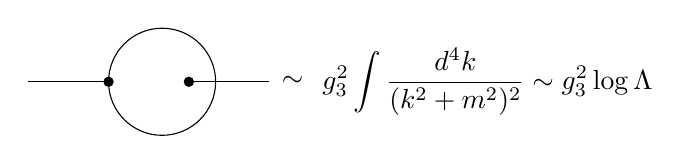
\begin{tikzpicture}[baseline=(eq.base),scale=.85]
  \coordinate (eq) at (0,0);
  \draw (-2.8,0)--(-1.6,0);
  \draw (-.4,0)--(.8,0);
  \draw (-1.6,0) arc (180:0:.8);
  \draw (-1.6,0) arc (-180:0:.8);
  \fill (-1.6,0) circle (2.2pt);
  \fill (-.4,0) circle (2.2pt);
  \node at (1.15,0) {\(\sim\)};
  \node[anchor=west] at (1.45,0)
  {\(\displaystyle
    g_3^2\int \frac{d^4k}{(k^2+m^2)^2}
    \sim g_3^2\log\Lambda\)} ;
\end{tikzpicture}
\]
and this divergent contribution to the mass term in the self-energy is
canceled by a mass counterterm,
\[
  \delta m^2\sim g_3^2\log\Lambda .
\]
On the other hand,
\[
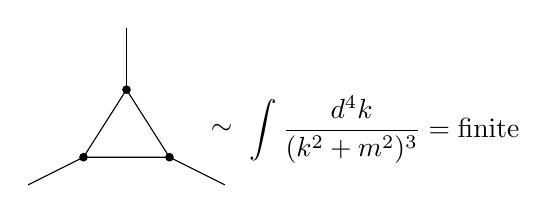
\begin{tikzpicture}[baseline=(tri.base),scale=.78]
  \coordinate (tri) at (0,0);
  \coordinate (a) at (-.7,-.45);
  \coordinate (b) at (.7,-.45);
  \coordinate (c) at (0,.65);
  \draw (a)--(b)--(c)--cycle;
  \draw (a)--++(-.9,-.45);
  \draw (b)--++(.9,-.45);
  \draw (c)--++(0,1);
  \fill (a) circle (2pt);
  \fill (b) circle (2pt);
  \fill (c) circle (2pt);
  \node at (1.55,0) {\(\sim\)};
  \node[anchor=west] at (1.85,0)
  {\(\displaystyle
    \int \frac{d^4k}{(k^2+m^2)^3}=\hbox{finite}\)} ;
\end{tikzpicture}
\]
and the corresponding box graph is finite as well.  Thus no counterterms of
the form \(\delta g_4\phi^4,\delta g_6\phi^6,\ldots\) are needed in this
example.

Next consider \(D=4\), with
\[
  S[\phi]\supset \int d^4x\,g_4\phi^4 .
\]
The tadpole correction is quadratically divergent,
\[
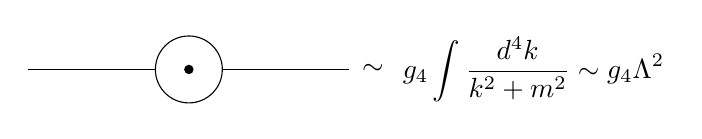
\begin{tikzpicture}[baseline=(eq.base),scale=.85]
  \coordinate (eq) at (0,0);
  \draw (-2.4,0)--(-.5,0);
  \draw (.5,0)--(2.4,0);
  \draw (0,0) circle (.5);
  \fill (0,0) circle (2pt);
  \node at (2.75,0) {\(\sim\)};
  \node[anchor=west] at (3.05,0)
  {\(\displaystyle
    g_4\int \frac{d^4k}{k^2+m^2}\sim g_4\Lambda^2\)} ;
\end{tikzpicture}
\]
so a mass counterterm is required,
\[
  \delta m^2\sim g_4\Lambda^2+O(g_4^2).
\]
At the next order the momentum-dependent part of the two-point function
requires a wavefunction counterterm,
\[
  \delta Z\,(\partial\phi)^2,\qquad
  \delta Z\sim g_4^2\log\Lambda .
\]
The four-point fish graph is also logarithmically divergent,
\[
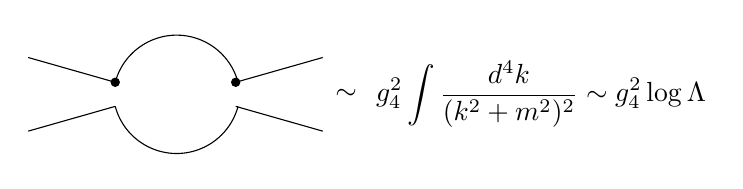
\begin{tikzpicture}[baseline=(eq.base),scale=.85]
  \coordinate (eq) at (0,0);
  \draw (-2.2,.55)--(-.9,.18);
  \draw (-2.2,-.55)--(-.9,-.18);
  \draw (.9,.18)--(2.2,.55);
  \draw (.9,-.18)--(2.2,-.55);
  \draw (-.9,.18) arc (165:15:.95);
  \draw (-.9,-.18) arc (-165:-15:.95);
  \fill (-.9,.18) circle (2pt);
  \fill (.9,.18) circle (2pt);
  \node at (2.55,0) {\(\sim\)};
  \node[anchor=west] at (2.85,0)
  {\(\displaystyle
    g_4^2\int \frac{d^4k}{(k^2+m^2)^2}
    \sim g_4^2\log\Lambda\)} ;
\end{tikzpicture}
\]
and hence
\[
  \delta g_4\sim g_4^2\log\Lambda .
\]
No counterterms \(\delta g_6\phi^6,\ldots\) are needed.

Finally take \(D=4\), with
\[
  S[\phi]\supset \int d^4x\,g_6\phi^6 .
\]
Now a logarithmically divergent eight-point counterterm is generated:
\[
  \delta g_8\phi^8,\qquad
  \delta g_8\sim g_6^2\log\Lambda .
\]
Even after subtracting divergent subdiagrams, further logarithmic divergences
generate
\[
  \delta g_{10}\phi^{10},\qquad
  \delta g_{10}\sim g_6^3\log\Lambda ,
\]
and so on without end.

Superficially, the necessary counterterms are dictated by dimensional
analysis.  The action \(S[\phi]\) is dimensionless, and the scalar field has
mass dimension
\[
  [\phi]=\frac{D-2}{2}.
\]
An operator \(O_I\) made of \(n\) powers of \(\phi\) and \(\ell\) derivatives
has mass dimension
\[
  d_I=\ell+n\frac{D-2}{2}.
\]
Thus \(g_I\) has mass dimension \(D-d_I\).

For
\[
  O_I=\partial^{\ell_1}\phi\cdots \partial^{\ell_n}\phi ,
\]
the corresponding effective coupling \(g_I^{\rm eff}\) is computed from
\[
  \left.
  \frac{\partial^{\ell_1}}{\partial k_1^{\ell_1}}
  \cdots
  \frac{\partial^{\ell_n}}{\partial k_n^{\ell_n}}
  \Gamma^{(n)}(k_1,\ldots,k_{n-1})
  \right|_{k_i=0},
  \qquad
  k_n=-k_1-\cdots-k_{n-1}.
\]
Assuming the answer is nonsingular as \(m\to0\), a UV-divergent contribution
from a one-particle-irreducible diagram has the schematic form
\[
  \prod_J g_J^{V_J}\,
  \Lambda^{\,D-d_I-\sum_J V_J(D-d_J)}
  (\log\Lambda)^{\#\ {\rm loops}} .
\]
Therefore a potentially divergent counterterm \(\delta g_I O_I\) is needed
in the action only if
\[
  D-d_I-\sum_J V_J(D-d_J)\ge 0 .
\]

If \(d_I\le D\) for every coupling \(g_IO_I\) appearing in
\(\widetilde S[\phi]\), then potentially only counterterms for operators with
\(d_I\le D\) are needed in order to make \(\Gamma[\phi]\) finite.  Such a
theory is renormalizable.

If, however, \(S[\phi]\) contains some interaction \(g_JO_J\) with
\(d_J>D\), then infinitely many counterterms \(\delta g_IO_I\) are needed,
with \(d_I\) arbitrarily large.  In that case one cannot produce a finite
\(\Gamma[\phi]\) with only finitely many terms in \(\widetilde S[\phi]\).
The theory is nonrenormalizable, and it cannot be pinned down completely by
measuring only finitely many physical couplings \(\lambda_{\rm phys}\).

\subsection[Cancellation of Divergences in D=6 phi3 Theory]
{Cancellation of Divergences in \(D=6\) \(\phi^3\) Theory}

Let us understand in more detail the cancellation of divergences in a
renormalizable theory.  As an example, consider \(D=6\) \(\phi^3\) theory:
\[
\begin{split}
  {\cal L}_E
  ={}&\frac{1}{2}(\partial_\mu\phi)^2
      +\frac{1}{2}m_R^2\phi^2
      +\delta Z\left[
        \frac{1}{2}(\partial_\mu\phi)^2
        +\frac{1}{2}m_R^2\phi^2
      \right]  \\
   &+\frac{1}{2}\delta m^2\phi^2
      +\frac{1}{3!}g_R\phi^3
      +\frac{1}{3!}\delta g\,\phi^3 .
\end{split}
\]
The two-point one-particle-irreducible graph is
\[
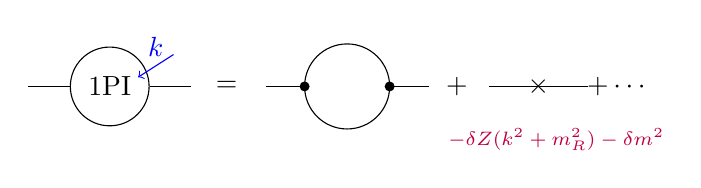
\begin{tikzpicture}[baseline=(eq.base),scale=.9]
  \coordinate (eq) at (0,0);
  \node[draw,circle,minimum size=1.0cm] (ipi) at (-3.1,0) {1PI};
  \draw (-4.25,0)--(ipi.west);
  \draw (ipi.east)--(-1.95,0);
  \draw[->,blue] (-2.2,.45)--(-2.7,.13) node[midway,above] {\(k\)};
  \node at (-1.45,0) {\(=\)};
  \draw (-.9,0)--(-.35,0);
  \draw (.85,0)--(1.4,0);
  \draw (-.35,0) arc (180:0:.6);
  \draw (-.35,0) arc (-180:0:.6);
  \fill (-.35,0) circle (2pt);
  \fill (.85,0) circle (2pt);
  \node at (1.8,0) {\(+\)};
  \draw (2.25,0)--(3.65,0);
  \node at (2.95,0) {\(\times\)};
  \node[purple,align=center,font=\scriptsize] at (3.2,-.75)
    {\(-\delta Z(k^2+m_R^2)-\delta m^2\)};
  \node at (4.05,0) {\(+\cdots\)};
\end{tikzpicture}
\]
with the one-loop contribution
\[
  \frac{1}{2}g_R^2
  \int\frac{d^6\ell}{(2\pi)^6}\,
  \frac{1}{
    (\ell^2+m_R^2)((k-\ell)^2+m_R^2)
  } .
\]
In a momentum cutoff scheme,
\[
  \delta m^2\sim g_R^2\Lambda^2
  +g_R^2m_R^2\log\Lambda,
  \qquad
  \delta Z\sim g_R^2\log\Lambda .
\]
In dimensional regularization, with \(D=6-\epsilon\),
\[
  \delta m^2\sim g_R^2m_R^2\frac{1}{\epsilon},
  \qquad
  \delta Z\sim g_R^2\frac{1}{\epsilon}.
\]

It will be useful later to inspect the explicit \(k\)-dependence of the
one-loop contribution to \(\Sigma(k)\):
\[
\begin{split}
  I(k)
  &=
  \frac{1}{2}g_R^2
  \int\frac{d^D\ell}{(2\pi)^D}\int_0^1 dx\,
  \frac{1}{
    \bigl(\ell^2+k^2x(1-x)+m_R^2\bigr)^2
  }  \\
  &=
  \frac{1}{2}g_R^2
  \frac{\Gamma(2-\frac{D}{2})}{(4\pi)^{D/2}}
  \int_0^1 dx\,
  \bigl(k^2x(1-x)+m_R^2\bigr)^{D/2-2}.
\end{split}
\]
For \(D=6-\epsilon\),
\[
\begin{split}
  I(k)
  =\frac{g_R^2}{2(4\pi)^3}\bigg[
  &\frac{1}{\epsilon}
    \left(-\frac{8}{3}k^2-16m_R^2\right)
   +\left(\frac{4}{3}k^2+8m_R^2\right)\log(k^2)  \\
  &+\#\,k^2+\#\,m_R^2
   +\hbox{terms that vanish at large }k
  \bigg].
\end{split}
\]
Thus one may choose
\[
  \left.\delta Z\right|_{O(g_R^2)}
  =
  \frac{g_R^2}{2(4\pi)^3}
  \left(-\frac{8}{3}\frac{1}{\epsilon}
  +\hbox{finite}\right),
\]
and
\[
  \left.\delta m_R^2\right|_{O(g_R^2)}
  =
  \frac{g_R^2m_R^2}{2(4\pi)^3}
  \left(-\frac{40}{3}\frac{1}{\epsilon}
  +\hbox{finite}\right).
\]
After canceling the \(1/\epsilon\) terms, the finite self-energy behaves at
large \(k\) as
\[
  \left.\Sigma(k)\right|_{O(g_R^2)}
  \sim (\alpha k^2+\beta)\log(k^2),
  \qquad k^2\gg m_R^2 .
\]

For the three-point function,
\[
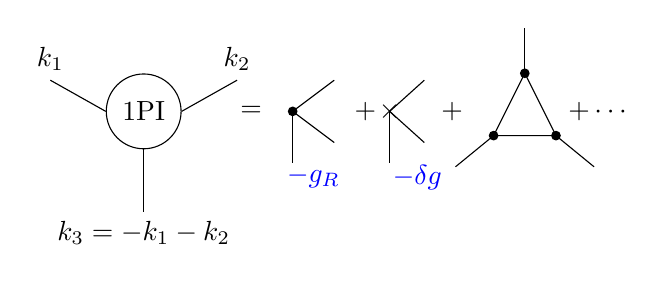
\begin{tikzpicture}[baseline=(eq.base),scale=.88]
  \coordinate (eq) at (0,0);
  \node[draw,circle,minimum size=.95cm] (ipi) at (-3.5,0) {1PI};
  \draw (ipi.west)--++(-.8,.45) node[above] {\(k_1\)};
  \draw (ipi.east)--++(.8,.45) node[above] {\(k_2\)};
  \draw (ipi.south)--++(0,-.9) node[below] {\(k_3=-k_1-k_2\)};
  \node at (-1.95,0) {\(=\)};
  \draw (-1.35,0)--(-.75,.45);
  \draw (-1.35,0)--(-.75,-.45);
  \draw (-1.35,0)--(-1.35,-.75);
  \fill (-1.35,0) circle (2pt);
  \node[blue] at (-1.05,-.95) {\(-g_R\)};
  \node at (-.3,0) {\(+\)};
  \draw (.05,0)--(.55,.45);
  \draw (.05,0)--(.55,-.45);
  \draw (.05,0)--(.05,-.75);
  \node at (.05,0) {\(\times\)};
  \node[blue] at (.45,-.95) {\(-\delta g\)};
  \node at (.95,0) {\(+\)};
  \coordinate (a) at (1.55,-.35);
  \coordinate (b) at (2.45,-.35);
  \coordinate (c) at (2.0,.55);
  \draw (a)--(b)--(c)--cycle;
  \draw (a)--++(-.55,-.45);
  \draw (b)--++(.55,-.45);
  \draw (c)--++(0,.65);
  \fill (a) circle (2pt);
  \fill (b) circle (2pt);
  \fill (c) circle (2pt);
  \node at (3.05,0) {\(+\cdots\)};
\end{tikzpicture}
\]
and the triangle graph gives
\[
  -g_R^3
  \int\frac{d^6\ell}{(2\pi)^6}\,
  \frac{1}{
    (\ell^2+m_R^2)
    ((\ell+k_1)^2+m_R^2)
    ((\ell+k_2)^2+m_R^2)
  } .
\]
Therefore
\[
  \delta g\sim g_R^3\log\Lambda
  \qquad\hbox{or}\qquad
  \delta g\sim g_R^3\frac{1}{\epsilon}.
\]
The four-point one-particle-irreducible graph at this order is finite.

At the next order in perturbation theory, the two-point function contains
two-loop graphs and counterterm insertions:
\[
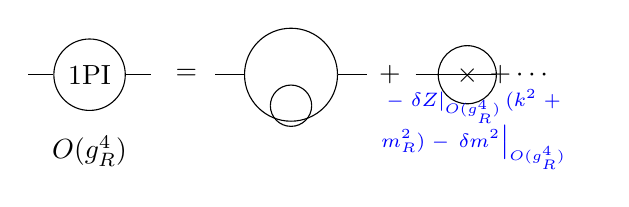
\begin{tikzpicture}[baseline=(eq.base),scale=.82]
  \coordinate (eq) at (0,0);
  \node[draw,circle,minimum size=.9cm] (ipi) at (-3.4,0) {1PI};
  \draw (-4.35,0)--(ipi.west);
  \draw (ipi.east)--(-2.45,0);
  \node[below] at (-3.4,-.8) {\(O(g_R^4)\)};
  \node at (-1.9,0) {\(=\)};
  \draw (-1.45,0)--(-1.0,0);
  \draw (.45,0)--(.9,0);
  \draw (-1.0,0) arc (180:0:.72);
  \draw (-1.0,0) arc (-180:0:.72);
  \draw (-.6,-.48) arc (180:0:.32);
  \draw (-.6,-.48) arc (-180:0:.32);
  \node at (1.25,0) {\(+\)};
  \draw (1.65,0)--(2.9,0);
  \draw (2.0,0) arc (180:0:.45);
  \draw (2.0,0) arc (-180:0:.45);
  \node at (2.45,-.02) {\(\times\)};
  \node at (3.25,0) {\(+\cdots\)};
  \node[blue,font=\scriptsize,align=center,text width=3.0cm] at (2.55,-.85)
  {\(-\left.\delta Z\right|_{O(g_R^4)}(k^2+m_R^2)
    -\left.\delta m^2\right|_{O(g_R^4)}\)};
\end{tikzpicture}
\]
The issue is that some of the graphs contain a divergent self-energy
subdiagram.  Schematically,
\[
\begin{tikzpicture}[baseline=(eq.base),scale=.78]
  \coordinate (eq) at (0,0);
  \draw (-2.0,0)--(-1.1,0);
  \draw (1.1,0)--(2.0,0);
  \draw (-1.1,0) arc (180:0:1.1);
  \draw (-1.1,0) arc (-180:0:1.1);
  \node[draw,ellipse,minimum width=.65cm,minimum height=.45cm] at (0,-.78)
    {\(\Sigma\)};
  \draw (-.5,-.35) arc (180:0:.5);
  \node at (2.45,0) {\(\sim\)};
  \node[anchor=west] at (2.8,0)
  {\(\displaystyle
    \int\frac{d^6q}{(2\pi)^6}
    \frac{\Sigma(q)}
    {(q^2+m_R^2)^2((k-q)^2+m_R^2)}
  \)};
\end{tikzpicture}
\]
where the dressed propagator in the indicated subdiagram has
\[
  G(q)=\frac{1}{q^2+m_R^2-\Sigma(q)}.
\]
At large \(q\),
\[
  \left.\Sigma(q)\right|_{O(g_R^2)}
  \sim (\alpha q^2+\beta)\log\!\left(\frac{q^2}{M^2}\right),
\]
for some finite \(\alpha,\beta,M\).  The UV divergence has simple
\(k\)-dependence, because
\[
\begin{split}
  \int\frac{d^6q}{(2\pi)^6}
  \frac{\Sigma(q)}{(q^2+m_R^2)^2}
  \bigg[
  &\frac{1}{(k-q)^2+m_R^2}
  -\frac{1}{q^2+m_R^2}  \\
  &-\frac{2k\cdot q-k^2}{(q^2+m_R^2)^2}
  -\frac{4(k\cdot q)^2}{(q^2+m_R^2)^3}
  \bigg]
  =\hbox{finite}.
\end{split}
\]

Let us verify the same statement in dimensional regularization.  Using the
Feynman trick, the relevant integral can be written in the form
\[
  \int\frac{d^Dq}{(2\pi)^D}\int_0^1 dx\,
  \frac{2(1-x)\Sigma(q+kx)}
       {(q^2+k^2x(1-x)+m_R^2)^3}.
\]
The divergent part of the \(q\)-integral, including
\(\Sigma(q)\sim(\alpha q^2+\beta)\log(q^2/M^2)\), can be evaluated using
\[
  \int\frac{d^Dq}{(2\pi)^D}
  \frac{1}{(q^2+\Delta)^n}
  =
  \frac{1}{(4\pi)^{D/2}}
  \frac{\Gamma(n-\frac{D}{2})}{\Gamma(n)}
  \Delta^{D/2-n},
\]
and
\[
  \int\frac{d^Dq}{(2\pi)^D}
  \frac{\log(q^2+\Delta)}{(q^2+\Delta)^n}
  =
  -\frac{1}{(4\pi)^{D/2}}
  \frac{\partial}{\partial n}
  \left[
    \frac{\Gamma(n-\frac{D}{2})}{\Gamma(n)}
    \Delta^{D/2-n}
  \right].
\]
For \(D=6-\epsilon\), \(n=2,3\), this gives schematically
\[
  \sim
  \frac{\partial}{\partial\epsilon}
  \left[
    \left(\frac{\#}{\epsilon}+\#\log\Delta\right)
    \Delta^{3-n}
  \right]
  +\frac{\#}{\epsilon}\Delta^{3-n}
  +\hbox{finite}
  \sim
  \left(\frac{\#}{\epsilon^2}+\frac{\#}{\epsilon}\right)
  \Delta^{3-n}
  +\hbox{finite}.
\]
Importantly, there is no \(\epsilon^{-1}\log\Delta\) term.  This leads to
\[
  D=6-\epsilon:\qquad
  A_\epsilon k^2+B_\epsilon+\hbox{finite},
\]
where
\[
  A_\epsilon=\frac{\alpha_1}{\epsilon}+\frac{\alpha_2}{\epsilon^2},
  \qquad
  B_\epsilon=\frac{\beta_1}{\epsilon}+\frac{\beta_2}{\epsilon^2},
\]
for finite \(k\)-independent constants
\(\alpha_1,\alpha_2,\beta_1,\beta_2\).  These divergences are canceled by
including \(\delta Z\) and \(\delta m^2\) counterterms of order
\[
  \frac{g_R^4}{\epsilon^2}
  \qquad\hbox{and}\qquad
  \frac{g_R^4}{\epsilon}.
\]
If a divergence of the form
\[
  \frac{1}{\epsilon}\log(k^2)
\]
had appeared, there would be no counterterm in a local Lagrangian that could
cancel it.  Luckily, this does not occur.

\subsection{Subdivergences and BPHZ Subtractions}

Next, let us inspect the UV divergence of the diagram
\[
\begin{tikzpicture}[baseline=(eq.base),scale=.82]
  \coordinate (eq) at (0,0);
  \coordinate (L) at (-1.2,0);
  \coordinate (R) at (1.2,0);
  \coordinate (T) at (0,.95);
  \coordinate (B) at (0,-.95);
  \draw (-2.1,0)--(L);
  \draw (R)--(2.1,0);
  \draw (L)--(T)--(R)--(B)--cycle;
  \draw (T)--(B);
  \fill (L) circle (2pt);
  \fill (R) circle (2pt);
  \fill (T) circle (2pt);
  \fill (B) circle (2pt);
  \node[blue] at (-1.9,.25) {\(k\)};
  \node[blue] at (-.35,.72) {\(\ell_2\)};
  \node[blue] at (.45,.72) {\(\ell_1\)};
  \node[blue] at (-.55,-.72) {\(k-\ell_2\)};
  \node[blue] at (.75,-.72) {\(k-\ell_1\)};
  \node at (2.55,0) {\(=\)};
  \node[anchor=west] at (2.95,0) {\(\displaystyle
    \frac{g_R^4}{2}
    \int\frac{d^6\ell_1}{(2\pi)^6}
        \frac{d^6\ell_2}{(2\pi)^6}
    P(\ell_1)P(k-\ell_1)P(\ell_2)P(k-\ell_2)P(\ell_1-\ell_2)
  \)};
\end{tikzpicture}
\]
where
\[
  P(k)=\frac{1}{k^2+m_R^2}
      =\int_0^\infty d\alpha\,e^{-\alpha(k^2+m_R^2)} .
\]
Thus the loop integral can be written as
\[
\begin{split}
  &\int_0^\infty\prod_{i=1}^5 d\alpha_i\,
    e^{-m_R^2\sum_i\alpha_i}
  \int\frac{d^6\ell_1}{(2\pi)^6}
      \frac{d^6\ell_2}{(2\pi)^6}  \\
  &\quad\times
  \exp\!\left[
    -\alpha_1\ell_1^2
    -\alpha_2(k-\ell_1)^2
    -\alpha_3\ell_2^2
    -\alpha_4(k-\ell_2)^2
    -\alpha_5(\ell_1-\ell_2)^2
  \right]  \\
  &=
  \frac{1}{(4\pi)^6}
  \int_0^\infty\prod_{i=1}^5 d\alpha_i\,
  e^{-m_R^2\sum_i\alpha_i}
  \frac{e^{-k^2Q}}{(\det A)^3}.
\end{split}
\]
Here
\[
  A=
  \begin{pmatrix}
    \alpha_1+\alpha_2+\alpha_5 & -\alpha_5\\
    -\alpha_5 & \alpha_3+\alpha_4+\alpha_5
  \end{pmatrix},
\]
and
\[
  Q=\alpha_2+\alpha_4
  -(\alpha_2,\alpha_4)A^{-1}
  \begin{pmatrix}\alpha_2\\ \alpha_4\end{pmatrix}
  \ge 0 .
\]
The UV divergence comes from the region \(\det A\to0\).

The generic subdivergences occur in the limits
\[
  \alpha_1,\alpha_2,\alpha_5\to0,
  \qquad\hbox{or}\qquad
  \alpha_3,\alpha_4,\alpha_5\to0,
\]
which are canceled by the corresponding counterterm diagrams for the nested
one-loop subgraphs.  Writing the integral in the form
\[
  \int_0^\infty\prod_i d\alpha_i\,
  e^{-m_R^2\sum_i\alpha_i}
  F(k^2;\alpha_1,\ldots,\alpha_5),
  \qquad
  F=\frac{e^{-k^2Q}}{(\det A)^3},
\]
we note the scaling relation
\[
  \rho^6 F\!\left(
    \frac{k^2}{\rho};
    \rho\alpha_1,\ldots,\rho\alpha_5
  \right)
  =
  F(k^2;\alpha_1,\ldots,\alpha_5).
\]
The effect of adding the two subdivergence counterterms amounts to replacing
\(F\) with
\[
\begin{split}
  \widetilde F
  ={}&F
  -\lim_{\rho\to0}
   \rho^3F(k^2;\rho\alpha_1,\rho\alpha_2,\alpha_3,\alpha_4,\rho\alpha_5)
  \\
  &-\lim_{\rho\to0}
   \rho^3F(k^2;\alpha_1,\alpha_2,\rho\alpha_3,\rho\alpha_4,\rho\alpha_5).
\end{split}
\]

The remaining divergence in the integral of \(\widetilde F\) comes from the
simultaneous limit
\[
  \alpha_1,\ldots,\alpha_5\to0,
\]
and by power counting it depends on \(k\) at most quadratically.  After
canceling this divergence by adjusting \(\delta Z\) and \(\delta m^2\), we are
left with
\[
\begin{split}
  \int\left[\prod_i d\alpha_i\,e^{-m_R^2\alpha_i}\right]
  \bigg(
  \widetilde F
  -\left.\widetilde F\right|_{k^2=0}
  -\left.
    \frac{\partial\widetilde F}{\partial k^2}
   \right|_{k^2=0}k^2
  \bigg),
\end{split}
\]
and one can verify that this integral is finite.

This analysis can be extended to show that all divergences in 1PI diagrams can
be canceled by diagrams involving counterterms that correspond to nested
subdiagrams.  This proves perturbative renormalizability of
naive-power-counting-renormalizable theories.  This is the
Bogoliubov-Parasiuk-Hepp-Zimmermann theorem.

\section{Renormalization Group}

The renormalization group is a way of characterizing a QFT by effective
descriptions at different energy or momentum scales.  It is also a
computational scheme for relating such descriptions at different scales.

There are two standard formulations.
\begin{itemize}
\item The ``1PI RG'', also called the Gell-Mann--Low equation or the
Callan--Symanzik equation, is an improved version of perturbation theory.
It recycles the computation of loop corrections in subdiagrams and performs a
partial resummation.
\item The Wilsonian RG, also called the Wilson--Polchinski equation, defines a
Wilsonian effective action \(S_\Lambda[\phi]\) by performing the functional
integral over modes \(\widetilde\phi(k)\) with
\(\Lambda<|k|<\Lambda_0\), where \(\Lambda_0\) is a finite UV cutoff.  One
then studies how \(S_\Lambda[\phi]\) changes with \(\Lambda\).
\end{itemize}

\begin{center}
\begin{tikzpicture}[>=Stealth,scale=0.9]
  \begin{scope}
    \coordinate (A) at (-0.75,0);
    \coordinate (B) at (0.75,0);
    \draw (-1.55,0.82)--(A)--(-1.55,-0.82);
    \draw (1.55,0.82)--(B)--(1.55,-0.82);
    \fill (A) circle (1.8pt);
    \fill (B) circle (1.8pt);
    \node at (0,-1.25) {tree};
  \end{scope}
  \draw[->] (2.0,0) -- (2.7,0);
  \begin{scope}[xshift=4.0cm]
    \coordinate (A) at (-0.85,0);
    \coordinate (B) at (0.85,0);
    \draw (-1.65,0.82)--(A)--(-1.65,-0.82);
    \draw (1.65,0.82)--(B)--(1.65,-0.82);
    \draw (A) .. controls (-0.15,0.75) and (0.15,0.75) .. (B);
    \draw (A) .. controls (-0.15,-0.75) and (0.15,-0.75) .. (B);
    \fill (A) circle (1.8pt);
    \fill (B) circle (1.8pt);
    \node at (0,-1.25) {one loop};
  \end{scope}
  \draw[->] (6.0,0) -- (6.7,0);
  \begin{scope}[xshift=8.1cm]
    \coordinate (A) at (-1.0,0);
    \coordinate (B) at (0.3,0);
    \coordinate (C) at (1.35,0);
    \draw (-1.75,0.82)--(A)--(-1.75,-0.82);
    \draw (1.95,0.82)--(C)--(1.95,-0.82);
    \draw (A) .. controls (-0.6,0.75) and (-0.1,0.75) .. (B);
    \draw (A) .. controls (-0.6,-0.75) and (-0.1,-0.75) .. (B);
    \draw (B) .. controls (0.65,0.65) and (0.95,0.65) .. (C);
    \draw (B) .. controls (0.65,-0.65) and (0.95,-0.65) .. (C);
    \draw[orange,line width=1.1pt,rounded corners] (-1.18,-0.92) rectangle (0.48,0.92);
    \fill (A) circle (1.8pt);
    \fill (B) circle (1.8pt);
    \fill (C) circle (1.8pt);
    \node[align=center] at (0,-1.35) {subdiagram\\reused};
  \end{scope}
\end{tikzpicture}
\end{center}

The mechanism is to define energy-scale-dependent effective, or
renormalized, couplings \(g(\mu)\), and then study how they vary with
\(\mu\).

\subsection[The Running Coupling in D=4 phi4 Theory]
{The Running Coupling in \(D=4\) \(\phi^4\) Theory}

Let us begin with \(D=4\) \(\phi^4\) theory.  The bare Euclidean Lagrangian is
\[
  {\cal L}_E
  =
  \frac{1}{2}(\partial\phi)^2+\frac{1}{2}m_0^2\phi^2
  +\frac{1}{4!}g_0\phi^4 .
\]
Equivalently, in terms of \(\phi_R=Z_R^{-1/2}\phi\),
\[
\begin{split}
  {\cal L}_E
  ={}&
  \frac{1}{2}(\partial\phi_R)^2+\frac{1}{2}m_R^2\phi_R^2
  +(Z_R-1)
  \left[
    \frac{1}{2}(\partial\phi_R)^2+\frac{1}{2}m_R^2\phi_R^2
  \right]  \\
  &+\frac{1}{2}\delta m^2\phi_R^2
  +\frac{1}{4!}g_R\phi_R^4
  +\frac{1}{4!}\delta g\,\phi_R^4 .
\end{split}
\]

Consider the amputated 1PI four-point function,
\[
  -\Gamma^{(4)}(k_1,k_2,k_3),
  \qquad k_4=-k_1-k_2-k_3,
\]
with external \(\phi_R\) lines.  It is tempting to define
\[
  g_R=-\Gamma^{(4)}(0,0,0),
\]
but this choice is arbitrary.  For a mass scale \(\mu\), one might expect
\(\Gamma^{(4)}\) with \(k_i\sim O(\mu)\) to characterize the effective
coupling strength at scale \(\mu\).  This is not quite accurate because the
normalization of \(\phi_R\) is still arbitrary.

The full propagator has the form
\[
  \frac{1}{k^2+m_R^2-\Sigma_R(k)} .
\]
Rescale the field by
\[
  Z(\mu)
  \equiv
  \left(
    1-\frac{\partial\Sigma_R}{\partial k^2}
  \right)^{-1}_{k^2=\mu^2}.
\]
Then the 1PI effective action \(\Gamma[\phi_R]\), viewed as a functional of
\[
  [\phi]_\mu\equiv Z(\mu)^{-1/2}\phi_R,
\]
has canonically normalized kinetic term for momentum \(k\sim O(\mu)\).

This gives a scale-dependent running coupling
\[
  g(\mu)
  =
  -\left(Z(\mu)^{1/2}\right)^4
  \Gamma^{(4)}(k_1,k_2,k_3)
  \bigg|_{k_i^2=\mu^2,\;s=t=u=-\frac{4}{3}\mu^2},
\]
where the symmetric Euclidean subtraction point specifies a renormalization
scheme.

At one loop, the tadpole correction to the two-point function does not affect
either \(Z_R\) or \(Z(\mu)\).  Therefore
\[
  Z_R=Z(\mu)=1+O(g_R^2)
\]
for the present one-loop computation of the four-point coupling.  The
one-loop four-point function is
\[
  -g(\mu)
  =
  -g_R-\delta g
  +3\frac{g_R^2}{32\pi^2}
  \int_0^1\dd x\,
  \left[
    \log\frac{\Lambda^2}{m_R^2-sx(1-x)}-1
  \right]_{s=-\frac{4}{3}\mu^2}
  +O(g_R^3).
\]
By the convention
\[
  g_R=g(\mu=0),
\]
we fix \(\delta g\), and hence obtain
\[
  g(\mu)
  =
  g_R
  -\frac{3g_R^2}{32\pi^2}
  \int_0^1\dd x\,
  \log
  \frac{m_R^2}
       {m_R^2+\frac{4}{3}\mu^2x(1-x)}
  +O(g_R^3).
\]
This gives an unambiguous relation between physical couplings.  However, the
one-loop correction becomes large when \(\mu\gg m_R\).

One could compute more terms in perturbation theory, but they also grow when
\(\mu\gg m_R\).  Instead compare \(g(\mu)\) to \(g(\mu')\) with
\(\mu'\) close to \(\mu\):
\[
  g(\mu')
  =
  g(\mu)
  -\frac{3}{32\pi^2}g(\mu)^2
  \int_0^1\dd x\,
  \log
  \frac{m_R^2+\frac{4}{3}\mu^2x(1-x)}
       {m_R^2+\frac{4}{3}{\mu'}^2x(1-x)}
  +O(g(\mu)^3).
\]
The perturbative expansion in \(g(\mu)\) is more reliable when
\(\mu'\) is close to \(\mu\).  Taking \(\mu'=\mu+d\mu\) gives
\[
  \frac{\dd g(\mu)}{\dd\log\mu}
  =
  \frac{3}{16\pi^2}g(\mu)^2
  \int_0^1\dd x\,
  \frac{\frac{4}{3}\mu^2x(1-x)}
       {m_R^2+\frac{4}{3}\mu^2x(1-x)}
  +O(g(\mu)^3).
\]
For \(\mu\gg m_R\), this becomes the one-loop renormalization group equation
\[
  \frac{\dd g(\mu)}{\dd\log\mu}
  =
  \frac{3g(\mu)^2}{16\pi^2}+O(g(\mu)^3),
\]
with beta function
\[
  \beta(g)=\frac{3g^2}{16\pi^2}+O(g^3).
\]

The one-loop equation has solution
\[
  \frac{1}{g(\mu)}-\frac{1}{g(\mu')}
  =
  -\frac{3}{16\pi^2}\log\frac{\mu}{\mu'},
\]
or
\[
  g(\mu)
  =
  \frac{g(\mu')}
       {1-\frac{3}{16\pi^2}g(\mu')\log(\mu/\mu')}.
\]
This can be a good approximation even when
\(g(\mu')\log(\mu/\mu')\) is large, provided the running coupling remains
small along the interval of scales.  Although only a one-loop computation was
performed, the solution includes infinitely many powers of \(g(\mu')\) through
the RG resummation.

At the scale
\[
  \mu_0
  =
  \mu'\,
  \exp\left[
    \frac{16\pi^2}{3}\frac{1}{g(\mu')}
  \right],
\]
the one-loop RGE predicts \(g(\mu_0)=\infty\).  Equivalently,
\[
  g(\mu)
  =
  \frac{1}
       {\frac{3}{16\pi^2}\log(\mu_0/\mu)}.
\]

\begin{center}
\begin{tikzpicture}[>=Stealth,scale=0.95]
  \draw[->] (-3.2,0) -- (4.7,0) node[right] {\(\log\mu\)};
  \draw[->] (0,-0.15) -- (0,3.9) node[above] {\(g(\mu)\)};
  \draw[green!55!black,dashed,line width=0.9pt]
    (-3.0,0.65) .. controls (-1.0,0.78) and (1.2,0.9) .. (2.8,0.92);
  \draw[purple,dashed,line width=0.9pt] (3.0,0) -- (3.0,3.7);
  \node[purple,below] at (3.0,0) {\(\mu_0\)};
  \draw[blue,line width=1.2pt]
    (-3.0,0.25) .. controls (-1.7,0.35) and (-0.5,0.55) .. (0.8,0.92)
    .. controls (1.75,1.25) and (2.55,2.3) .. (2.95,3.65);
  \node[purple,align=left,anchor=west] at (3.25,2.2)
    {strong coupling:\\cannot trust\\one-loop RG};
  \draw[purple,->] (3.15,2.25) -- (2.7,2.55);
  \draw[decorate,decoration={brace,amplitude=5pt},green!55!black]
    (-3.0,-0.35) -- (0.9,-0.35);
  \node[green!55!black] at (-1.05,-0.78) {perturbation theory valid};
  \draw[decorate,decoration={brace,amplitude=5pt,mirror},gray]
    (1.25,-0.45) -- (3.0,-0.45);
  \node[gray,align=center] at (2.05,-0.95)
    {near \(\mu_0\),\\perturbation theory breaks down};
\end{tikzpicture}
\end{center}

Instead of a coupling constant, the \(D=4\) \(\phi^4\) theory is characterized
by a mass scale \(\mu_0\).  This is dimensional transmutation.  The theory is
weakly coupled at energy \(E\ll\mu_0\), but strongly coupled at
\(E\sim\mu_0\).  Perturbation theory is really an expansion in powers of
\[
  \left(\log\frac{\mu_0}{E}\right)^{-1}.
\]
As perturbative control is lost for \(E\gtrsim\mu_0\), it is unclear from
this definition alone whether the \(D=4\) \(\phi^4\) theory exists as a QFT
obeying locality and microcausality at arbitrarily short distance scales, or
whether it is even a well-defined quantum-mechanical system admitting exact
Poincare symmetry.

\subsection{Formulation of the 1PI Renormalization Group}

Consider a QFT defined through the Euclidean path integral
\[
  Z=\int[D\phi]\,\exp\left[-\int d^Dx\,{\cal L}_E\right],
\]
with the path integral defined using a UV regularization scheme.  Write
\[
  {\cal L}_E={\cal L}_{\rm kin}+\sum_I g_I O_I .
\]
The \(g_I\)'s are bare couplings; they contain counterterms, including those
coming from the field-renormalization factor \(Z_R\).

The 1PI effective action may be written schematically as
\[
  \Gamma[\phi]
  =
  S_{\rm kin}
  +\sum_n\frac{1}{n!}
  \int
  \Gamma^{(n)}(k_1,\ldots,k_{n-1})\,
  \widetilde\phi(k_1)\cdots
  \widetilde\phi(k_{n-1})
  \widetilde\phi\!\left(-\sum_{i=1}^{n-1}k_i\right).
\]
For an operator \(O_I\) of schematic form
\[
  \phi\,\partial_x^{\ell_1}\phi\cdots
  \partial_x^{\ell_{n-1}}\phi,
\]
with \(n\) fields and derivative indices contracted in some way, an
appropriate definition of the renormalized coupling \(g_I(\mu)\) is obtained
by expanding \(\Gamma^{(n)}\) in the external momenta around some
\(K_i\sim O(\mu)\):
\[
\begin{split}
  &\Gamma^{(n)}
  (K_1+\delta k_1,\ldots,K_{n-1}+\delta k_{n-1})
\\
  &\qquad
  =
  \sum_{\ell_1,\ldots,\ell_{n-1}}
  \Gamma^{(n;\ell_1,\ldots,\ell_{n-1})}
  (K_1,\ldots,K_{n-1})\,
  \delta k_1^{\ell_1}\cdots
  \delta k_{n-1}^{\ell_{n-1}},
\end{split}
\]
where the indices are again contracted in the pattern specified by \(O_I\).
Then define
\[
  g_I(\mu)
  :=
  -
  \left[Z(\mu)\right]^{n/2}
  \Gamma^{(n;\ell_1,\ldots,\ell_{n-1})}
  (k_1,\ldots,k_{n-1})
  \bigg|_{k_i\sim O(\mu)} .
\]
In naive, or unimproved, perturbation theory,
\[
  g_I(\mu)=g_I+\hbox{corrections},
\]
and the precise subtraction point is a choice of renormalization scheme.  The
field-strength factor is
\[
  Z(\mu)
  =
  \left(
    1-\frac{\partial\Sigma}{\partial k^2}
  \right)^{-1}_{k^2=\mu^2}.
\]

As a check, in the special case of the coupling
\[
  g_{2,2}\,\phi\,\Box\phi,
\]
we have
\[
  \Gamma^{(2;2)}\big|_{k^2=\mu^2}
  =
  \left.\frac{\partial\Sigma}{\partial k^2}\right|_{k^2=\mu^2}
  =
  1-\left(Z(\mu)\right)^{-1}.
\]
The corresponding renormalized coupling is therefore
\[
  g_{2,2}(\mu)
  =
  -Z(\mu)\left[1-\left(Z(\mu)\right)^{-1}\right]
  =
  1-Z(\mu),
\]
in agreement with the previous definition of \(Z(\mu)\).

Now express \(g_I(\mu')\) in terms of \(g_I(\mu)\) for
\(\mu'=\mu+\delta\mu\).  This relation is well-defined in the limit in which
the UV regulator is removed, for example \(\Lambda\to\infty\) or
\(\epsilon\to0\), and it gives only small logarithmic corrections for small
\(\delta\mu\).  This yields a 1PI RG equation of the form
\[
  \frac{\dd g_I(\mu)}{\dd\log\mu}
  =
  \beta_I(\{g_J(\mu)\};\mu).
\]

It is often preferable to introduce dimensionless running couplings
\[
  \lambda_I(\mu)\equiv \mu^{d_I-D}g_I(\mu),
\]
where \(d_I\) is the engineering dimension of \(O_I\).  For example, for a
mass term \(m_0^2\equiv g_2^{\rm bare}\),
\[
  \lambda_2(\mu)
  =
  \mu^{-2}Z(\mu)
  \left[
    g_2^{\rm bare}-\Sigma(k)\big|_{k^2=\mu^2}
  \right].
\]
The dimensionless couplings obey
\[
  \frac{\dd\lambda_I(\mu)}{\dd\log\mu}
  =
  \beta_I(\{\lambda_J(\mu)\}),
\]
with no further explicit \(\mu\)-dependence.

The job of the 1PI RG is to improve perturbation theory.  When comparing
physical observables at widely separated energy scales, naive perturbation
theory may break down because of large logarithms.  The RG-improved
perturbation theory, namely the expansion in running couplings obtained by
solving the RGE, may still be valid.

There is an important consistency check.  In formulating the RGE, we have
assumed renormalizability in relating \(g(\mu')\) to \(g(\mu)\).  In naive
perturbation theory in terms of a bare coupling \(g_0\), one may have
\[
  g(\mu)
  =
  g_0
  -b_1g_0^2\log\frac{\Lambda}{\mu}
  -b_2g_0^3\log\frac{\Lambda}{\mu}
  -c_1g_0^3\left(\log\frac{\Lambda}{\mu}\right)^2
  +O(g_0^4).
\]
Then
\[
  \frac{\dd g(\mu)}{\dd\log\mu}
  =
  b_1g_0^2+b_2g_0^3
  +2c_1g_0^3\log\frac{\Lambda}{\mu}
  +O(g_0^4).
\]
Re-expressing the result in terms of \(g(\mu)\), this becomes
\[
  b_1g(\mu)^2+b_2g(\mu)^3
  +2\left(c_1+b_1^2\right)
  g(\mu)^3\log\frac{\Lambda}{\mu}
  +O(g(\mu)^4).
\]
Consistency with renormalizability requires
\[
  c_1=-b_1^2.
\]

For example, in \(D=4\) \(\phi^4\) theory the double-logarithmic two-loop
four-point graphs are constrained by the one-loop coefficient:
\[
\begin{tikzpicture}[baseline=-0.45ex,scale=0.82]
  \coordinate (A) at (-0.85,0);
  \coordinate (B) at (0.05,0);
  \coordinate (C) at (0.95,0);
  \draw (-1.65,0.75)--(A)--(-1.65,-0.75);
  \draw (1.75,0.75)--(C)--(1.75,-0.75);
  \draw (A) .. controls (-0.55,0.6) and (-0.25,0.6) .. (B);
  \draw (A) .. controls (-0.55,-0.6) and (-0.25,-0.6) .. (B);
  \draw (B) .. controls (0.35,0.6) and (0.65,0.6) .. (C);
  \draw (B) .. controls (0.35,-0.6) and (0.65,-0.6) .. (C);
  \fill (A) circle (1.7pt);
  \fill (B) circle (1.7pt);
  \fill (C) circle (1.7pt);
\end{tikzpicture}
\quad+\quad
\begin{tikzpicture}[baseline=-0.45ex,scale=0.82]
  \coordinate (A) at (-0.9,0);
  \coordinate (B) at (0.9,0);
  \draw (-1.65,0.75)--(A)--(-1.65,-0.75);
  \draw (1.65,0.75)--(B)--(1.65,-0.75);
  \draw (A) .. controls (-0.25,0.75) and (0.25,0.75) .. (B);
  \draw (A) .. controls (-0.25,-0.75) and (0.25,-0.75) .. (B);
  \draw (0,0.75) .. controls (0.35,1.35) and (-0.35,1.35) .. (0,0.75);
  \fill (A) circle (1.7pt);
  \fill (B) circle (1.7pt);
\end{tikzpicture}
\quad+\hbox{permutations}
\sim
c_1g_0^3\left(\log\frac{\Lambda}{\mu}\right)^2
\]
with \(c_1=-b_1^2\).  The two-loop self-energy in this example contributes
only a single logarithm to \(\delta Z\).

Under a finite redefinition of the dimensionless coupling,
\[
  \widetilde\lambda(\mu)=f(\lambda(\mu)),
  \qquad
  f(\lambda)=\lambda+\alpha\lambda^2+\cdots,
\]
the RG equation is equivalently
\[
  \frac{\dd\lambda(\mu)}{\dd\log\mu}=\beta(\lambda(\mu)),
  \qquad
  \frac{\dd\widetilde\lambda(\mu)}{\dd\log\mu}
  =
  \widetilde\beta(\widetilde\lambda(\mu)).
\]
Therefore
\[
\begin{split}
  \beta(\lambda)
  &=
  \frac{\widetilde\beta(f(\lambda))}{f'(\lambda)}
\\
  &=
  \left(1-2\alpha\lambda+\cdots\right)
  \left(1+\alpha\lambda^2\frac{\partial}{\partial\lambda}+\cdots\right)
  \widetilde\beta(\lambda)
\\
  &=
  \widetilde\beta(\lambda)
  +\alpha\lambda
  \left(\lambda\frac{\partial}{\partial\lambda}-2\right)
  \widetilde\beta(\lambda)+\cdots .
\end{split}
\]
For a classically marginal coupling,
\[
  \beta(\lambda)=b_1\lambda^2+b_2\lambda^3+b_3\lambda^4+\cdots,
\]
and
\[
  \widetilde\beta(\lambda)
  =
  \widetilde b_1\lambda^2
  +\widetilde b_2\lambda^3
  +\widetilde b_3\lambda^4+\cdots.
\]
Thus the first two coefficients are scheme independent,
\[
  b_1=\widetilde b_1,\qquad b_2=\widetilde b_2,
\]
whereas
\[
  \widetilde b_3=b_3-\alpha b_2.
\]

\subsection{Renormalized Operators}

Consider an infinitesimal deformation of the action,
\[
  S\longrightarrow S+\delta S,
  \qquad
  \delta S=\int d^Dx\sum_I\delta g_I\,O_I .
\]
Correspondingly, the renormalized running couplings are deformed as
\[
  g_I(\mu)\longrightarrow g_I(\mu)+\delta g_I(\mu).
\]
The variations \(\delta g_I\) and \(\delta g_I(\mu)\) are linearly related:
\[
  \delta g_I
  =
  \sum_J\delta g_J(\mu)\,N_{JI}(\mu).
\]
The renormalized operator \([O_I]_\mu\) is defined by rewriting the deformation
as
\[
  \delta S=\int d^Dx\sum_I\delta g_I(\mu)\,[O_I]_\mu.
\]
Equivalently,
\[
  [O_I]_\mu=\sum_J N_{IJ}(\mu)O_J .
\]

In fact, the matrices \(N_{IJ}(\mu)\) are determined by the beta functions:
\[
\begin{split}
  0
  &\equiv
  \frac{\dd\,\delta g_I}{\dd\log\mu}
\\
  &=
  \sum_J
  \frac{\dd}{\dd\log\mu}
  \left[
    \delta g_J(\mu)N_{JI}(\mu)
  \right]
\\
  &=
  \sum_J
  \left[
    \delta\beta_J(g(\mu))\,N_{JI}(\mu)
    +\delta g_J(\mu)
    \frac{\dd N_{JI}(\mu)}{\dd\log\mu}
  \right].
\end{split}
\]
Thus
\[
  \frac{\dd N_{IJ}(\mu)}{\dd\log\mu}
  =
  -\sum_K \gamma_{IK}(g(\mu))N_{KJ}(\mu),
\]
where
\[
  \gamma_{IK}\equiv
  \frac{\partial\beta_K(g(\mu))}{\partial g_I(\mu)}.
\]
If an operator basis can be chosen in which \(\gamma_{IK}\) is diagonal, then
\[
  [O_I]_\mu
  =
  \exp\left[
    -\int_{\mu'}^\mu
    \frac{d\widetilde\mu}{\widetilde\mu}\,
    \gamma_I(g(\widetilde\mu))
  \right]
  [O_I]_{\mu'}.
\]
In a scale-invariant QFT, \(\gamma_I\) is constant, so
\[
  [O_I]_\mu
  =
  \left(\frac{\mu}{\mu'}\right)^{-\gamma_I}
  [O_I]_{\mu'}.
\]
In this case, \(\gamma_I\) is called the anomalous dimension of \(O_I\).

A special case is the field operator \(\phi\) itself.  Consider
\[
  \delta S=\int d^Dx\,\delta g_1\,\phi(x).
\]
The corresponding amputated 1PI insertion has no further corrections, and
the renormalized running coupling is
\[
  \delta g_1(\mu)
  =
  -\left(Z(\mu)\right)^{1/2}(\hbox{1PI insertion})
  =
  \left(Z(\mu)\right)^{1/2}\delta g_1 .
\]
Therefore
\[
  [\phi]_\mu=\left(Z(\mu)\right)^{-1/2}\phi.
\]
The anomalous dimension of \(\phi\) is
\[
  \gamma_\phi
  =
  -\frac{\dd\log\left[(Z(\mu))^{-1/2}\right]}{\dd\log\mu}
  =
  \frac{1}{2}\frac{\dd\log Z(\mu)}{\dd\log\mu}.
\]
In a scale-invariant theory,
\[
  \gamma_\phi=\hbox{constant}
  \qquad\Longleftrightarrow\qquad
  Z(\mu)\propto \mu^{2\gamma_\phi}.
\]

\subsection{Minimal Subtraction}

In the minimal-subtraction formulation of the 1PI RG, begin with a path
integral formulation of the QFT defined by dimensional regularization,
\[
  S
  =
  S_{\rm kin}
  +
  \int d^{d-\epsilon}x\,
  \sum_I g_I^\epsilon\,O_I(x).
\]
Here \(S_{\rm kin}\), for example, may contain
\(\frac12\int d^{d-\epsilon}x\,(\partial_\mu\phi)^2\).  The \(g_I^\epsilon\)
are bare couplings which depend on \(\epsilon\), while the \(O_I\) are bare
operators built out of \(\phi,\partial_\mu\phi,\ldots\).

The mass dimensions are
\[
  \begin{array}{c|c}
    & \hbox{mass dimension}
    \\ \hline
    \phi & \dfrac{d-\epsilon-2}{2}
    \\[0.6em]
    g_I^\epsilon & -\delta_I(\epsilon)
    \\[0.4em]
    O_I & d-\epsilon+\delta_I(\epsilon)
  \end{array}
\]
with
\[
  \delta_I(\epsilon)=\delta_I^{(0)}+\epsilon\,\delta_I^{(1)}
\]
by construction of \(O_I\).

Minimal subtraction is the renormalization scheme in which the dimensionless
renormalized running couplings \(\lambda_I(\mu)\) are defined so that the bare
coupling \(g_I^\epsilon\), expressed as a function of \(\lambda_J(\mu)\) and
\(\epsilon\), contains only negative powers of \(\epsilon\):
\[
  g_I^\epsilon
  =
  \mu^{-\delta_I(\epsilon)}
  \left[
    \lambda_I(\mu)
    +
    \sum_{n=1}^\infty
    \frac{1}{\epsilon^n}
    K_I^{(n)}\bigl(\{\lambda_J(\mu)\}\bigr)
  \right].
\]
The term with the \(K_I^{(n)}\)'s is the counterterm; it contains no
non-negative powers of \(\epsilon\).  This definition removes the freedom, or
ambiguity, in finite redefinitions of the \(\lambda_I(\mu)\), at least in
perturbation theory.

To see how the MS scheme works in practice, revisit \(d=4\) \(\phi^4\)
theory.  With dimensional regularization \(D=4-\epsilon\), the coupling in
the Euclidean Lagrangian is
\[
  {\cal L}_E\supset \frac{1}{4!}\,g^\epsilon\phi^4,
\]
whose mass dimension is
\[
  D-4\cdot\frac{D-2}{2}=\epsilon.
\]
In a generic renormalization scheme based on evaluating the 1PI diagram at
momenta of order \(\mu\), one would define the renormalized dimensionless
coupling \(\widetilde\lambda(\mu)\) by
\[
  \mu^\epsilon\widetilde\lambda(\mu)
  \equiv
  -\left(Z(\mu)\right)^2
  \left.
  \begin{tikzpicture}[baseline=-0.6ex,scale=0.55]
    \draw[line width=0.7pt] (0,0) circle (0.45);
    \node at (0,0) {\scriptsize 1PI};
    \draw[line width=0.7pt] (-0.85,0.65) -- (-0.32,0.32);
    \draw[line width=0.7pt] (-0.85,-0.65) -- (-0.32,-0.32);
    \draw[line width=0.7pt] (0.85,0.65) -- (0.32,0.32);
    \draw[line width=0.7pt] (0.85,-0.65) -- (0.32,-0.32);
  \end{tikzpicture}
  \right|_{\substack{k_i^2\sim O(\mu^2)\\
  s=-\mu^2 a_s,\ t=-\mu^2 a_t,\ u=-\mu^2 a_u}},
\]
for constants \(a_s,a_t,a_u\) of our choice.

At one loop this gives
\[
\begin{split}
  \mu^\epsilon\widetilde\lambda(\mu)
  &=
  g^\epsilon
  -
  \frac{(g^\epsilon)^2}{2}
  \int\frac{d^{4-\epsilon}k}{(2\pi)^{4-\epsilon}}
  \int_0^1 dx
\\
  &\hspace{2.5em}\times
  \left[
    \frac{1}{\left(k^2+\mu^2 a_s x(1-x)\right)^2}
    +(a_s\to a_t)+(a_s\to a_u)
  \right]
  +O(g^3)
\\
  &=
  g^\epsilon
  -
  \frac{(g^\epsilon)^2}{2}
  \mu^{-\epsilon}
  (4\pi)^{-2+\epsilon/2}
  \frac{
    \Gamma(\epsilon/2)\Gamma(1-\epsilon/2)^2
  }{
    \Gamma(2-\epsilon)
  }
  \left(a_s^{-\epsilon/2}+a_t^{-\epsilon/2}+a_u^{-\epsilon/2}\right)
  +O(g^3).
\end{split}
\]
Inverting this relation,
\[
\begin{split}
  g^\epsilon
  =
  \mu^\epsilon
  \bigg[
    \widetilde\lambda(\mu)
    &+
    \frac{\widetilde\lambda(\mu)^2}{2}
    (4\pi)^{-2+\epsilon/2}
    \frac{\Gamma(\epsilon/2)\Gamma(1-\epsilon/2)^2}
         {\Gamma(2-\epsilon)}
\\
    &\times
    \left(a_s^{-\epsilon/2}+a_t^{-\epsilon/2}+a_u^{-\epsilon/2}\right)
    +O(\widetilde\lambda^3)
  \bigg],
\end{split}
\]
or equivalently
\[
  g^\epsilon
  =
  \mu^\epsilon
  \left[
    \widetilde\lambda
    +
    \widetilde\lambda^2
    \left(
      \frac{3}{16\pi^2}\frac{1}{\epsilon}
      +\hbox{finite term depending on }a_s,a_t,a_u
    \right)
    +O(\widetilde\lambda^3)
  \right].
\]
In the MS scheme, \(\lambda(\mu)\) is instead defined so that
\[
  g^\epsilon
  =
  \mu^\epsilon
  \left[
    \lambda(\mu)
    +
    \lambda(\mu)^2\,
    \frac{3}{16\pi^2}\frac{1}{\epsilon}
    +O(\lambda^3)
  \right].
\]
Working in the MS scheme has the advantage of certain technical
simplifications: the nontrivial perturbative contributions to the
beta-functions are strictly of order \(\epsilon^0\).

To see this, inspect the RGE in MS:
\[
  g_I^\epsilon
  =
  \mu^{-\delta_I(\epsilon)}
  \left[
    \lambda_I(\mu)
    +
    \sum_{n\geq1}
    \epsilon^{-n}K_I^{(n)}(\lambda(\mu))
  \right].
\]
Because the bare coupling is independent of \(\mu\),
\[
\begin{split}
  0
  &\equiv
  \frac{\dd g_I^\epsilon}{\dd\log\mu}
\\
  &=
  -\delta_I\,\mu^{-\delta_I}
  \left[
    \lambda_I+\sum_{n\geq1}\epsilon^{-n}K_I^{(n)}
  \right]
  +
  \mu^{-\delta_I}
  \left[
    \beta_I^\epsilon
    +
    \sum_{n\geq1}
    \epsilon^{-n}
    \frac{\partial K_I^{(n)}}{\partial \lambda_J}
    \beta_J^\epsilon
  \right],
\end{split}
\]
where
\[
  \beta_I^\epsilon\equiv
  \frac{\dd\lambda_I(\mu)}{\dd\log\mu}
\]
is the beta-function in \(d-\epsilon\) dimensions.

A priori,
\[
  \beta_I^\epsilon
  =
  \sum_{m=0}^\infty \beta_I^{(m)}(\lambda)\,\epsilon^m
\]
is finite but has an all-orders expansion in \(\epsilon\).  As
\(\epsilon\to0\),
\[
  \beta_I^{(0)}(\lambda)\equiv \beta_I(\lambda)
\]
is the true beta-function of the QFT.

Organizing the preceding equation in powers of \(\epsilon\), we obtain
\[
\begin{split}
  0
  &=
  -\left(\delta_I^{(0)}+\epsilon\delta_I^{(1)}\right)
  \left[
    \lambda_I+\sum_{n\geq1}\epsilon^{-n}K_I^{(n)}
  \right]
  +
  \sum_{m\geq0}\epsilon^m\beta_I^{(m)}
\\
  &\hspace{2em}
  +
  \sum_{n\geq1}\sum_{m\geq0}
  \epsilon^{m-n}
  \frac{\partial K_I^{(n)}}{\partial\lambda_J}\,
  \beta_J^{(m)}.
\end{split}
\]
For example, the order \(\epsilon^1\) equation is
\[
  -\delta_I^{(1)}\lambda_I
  +
  \beta_I^{(1)}
  +
  \sum_{n\geq1}
  \frac{\partial K_I^{(n)}}{\partial\lambda_J}
  \beta_J^{(n+1)}
  =
  0,
\]
and the order \(\epsilon^2\) equation is
\[
  \beta_I^{(2)}
  +
  \sum_{n\geq1}
  \frac{\partial K_I^{(n)}}{\partial\lambda_J}
  \beta_J^{(n+2)}
  =
  0,
  \qquad\hbox{etc.}
\]
As \(n\) increases, \(K_I^{(n)}\) begins at higher order in \(\lambda\).
These relations can be satisfied in perturbation theory only if
\[
  \beta_I^{(m)}=0\quad(m\geq2),
  \qquad
  \beta_I^{(1)}=\delta_I^{(1)}\lambda_I.
\]
Thus
\[
  \beta_I^\epsilon
  =
  \beta_I^{(0)}(\lambda)
  +
  \epsilon\,\delta_I^{(1)}\lambda_I,
\]
as claimed.  The remaining equations at order \(\epsilon^{\leq0}\) determine
the \(K_I^{(n)}\)'s in terms of \(\beta_I^{(0)}\equiv\beta_I\) through the
recursive relations
\[
  \left(
    \beta_J\frac{\partial}{\partial\lambda_J}
    -\delta_I^{(0)}
  \right)K_I^{(n)}
  =
  \delta_I^{(1)}
  \left(
    1-\lambda_J\frac{\partial}{\partial\lambda_J}
  \right)K_I^{(n+1)},
  \qquad n\geq1,
\]
and
\[
  \beta_I-\delta_I^{(0)}\lambda_I
  =
  \delta_I^{(1)}
  \left(
    1-\lambda_J\frac{\partial}{\partial\lambda_J}
  \right)K_I^{(1)}.
\]

\subsection{The Trace of the Stress-Energy Tensor}

Recall that the stress-energy tensor \(T_{\mu\nu}(x)\) is the Noether current
associated with translation symmetry.  The action \(S[\phi]\) is invariant
under
\[
  \phi(x)\longrightarrow \phi'(x),
  \qquad
  \phi'(x')\equiv \phi(x),
  \qquad
  x'^\mu=x^\mu+\delta a^\mu.
\]
Thus
\[
  \delta\phi(x)
  =
  \phi'(x)-\phi(x)
  =
  -\delta a^\mu\partial_\mu\phi(x).
\]
The Noether procedure promotes the constant \(\delta a^\mu\) to
\(\delta a^\mu(x)\) and allows
\[
  \delta\phi(x)
  =
  -\delta a^\mu(x)\partial_\mu\phi(x)
  +
  \partial_\mu\delta a_\nu(x)\,D^{\mu\nu}\phi(x),
\]
where \(D^{\mu\nu}\) is to be chosen.  This is no longer a symmetry
variation, and in Euclidean convention
\[
  S[\phi+\delta\phi]
  =
  S[\phi]
  -
  \int d^Dx\,\partial_\mu\delta a_\nu(x)\,
  T_x^{\mu\nu}.
\]
The term proportional to \(\partial_\mu\delta a_\nu\) in \(\delta\phi\) only
affects \(T^{\mu\nu}\) by an equation-of-motion term.

Now consider the scaling transformation
\[
  \delta a^\mu(x)=\delta a\,x^\mu,
\]
which is not a symmetry in general.  Then
\[
  \delta S[\phi]
  =
  -\int d^Dx\,\delta a\,T^\mu{}_\mu(x),
\]
while the field transforms by
\[
  \delta\phi(x)
  =
  -\delta a\,x^\mu\partial_\mu\phi(x)
  +
  \delta a\,D^\mu{}_\mu\phi(x).
\]
We would like the massless free scalar action
\[
  S_{\rm kin}[\phi]=
  \int d^Dx\,\frac12(\partial_\mu\phi)^2
\]
to be invariant under the above scaling transformation.  This is satisfied
provided that
\[
  D^\mu{}_\mu=-\frac{D-2}{2},
  \qquad D=d-\epsilon.
\]
Equivalently,
\[
  \delta S_{\rm kin}[\phi]
  =
  \delta a\int d^Dx\,\partial_\mu\phi
  \left[
    -\partial_\mu(x^\nu\partial_\nu\phi)
    -\frac{D-2}{2}\partial_\mu\phi
  \right]
  =
  0
\]
up to a total derivative.

More generally, an operator \(O_I(x)\) made out of \(\phi(x)\) and its
derivatives, with mass dimension
\[
  d_I(\epsilon)\equiv d-\epsilon+\delta_I(\epsilon),
\]
transforms under scaling as
\[
  O_I'(x')
  =
  (1+\delta a)^{-d_I(\epsilon)}O_I(x).
\]
Therefore
\[
  S[\phi]
  =
  S_{\rm kin}[\phi]
  +
  \int d^{d-\epsilon}x\,
  \sum_I g_I^\epsilon O_I(x)
\]
obeys
\[
\begin{split}
  S[\phi']-S_{\rm kin}[\phi']
  &=
  \int d^{d-\epsilon}x'\,
  \sum_I g_I^\epsilon O_I'(x')
\\
  &=
  \int d^{d-\epsilon}x\,
  (1+\delta a)^{d-\epsilon}
  \sum_I
  g_I^\epsilon
  (1+\delta a)^{-d+\epsilon-\delta_I(\epsilon)}
  O_I(x)
\\
  &=
  \int d^{d-\epsilon}x\,
  \sum_I
  g_I^\epsilon
  (1+\delta a)^{-\delta_I(\epsilon)}
  O_I(x).
\end{split}
\]
Thus, up to a total derivative,
\[
  T^\mu{}_\mu(x)
  =
  \sum_I\delta_I(\epsilon)g_I^\epsilon O_I(x).
\]

It is more illuminating to re-express the right-hand side in terms of
renormalized quantities.  In the MS scheme,
\[
  g_I^\epsilon
  =
  \mu^{-\delta_I(\epsilon)}
  \left[
    \lambda_I(\mu)
    +
    \sum_{n\geq1}\epsilon^{-n}K_I^{(n)}(\lambda(\mu))
  \right].
\]
Because \(g_I^\epsilon\) is \(\mu\)-independent,
\[
  0
  =
  \frac{\dd g_I^\epsilon}{\dd\log\mu}
  =
  -\delta_I(\epsilon)g_I^\epsilon
  +
  \sum_J
  \frac{\dd\lambda_J(\mu)}{\dd\log\mu}
  \frac{\partial g_I^\epsilon}{\partial\lambda_J}.
\]
Using
\[
  \frac{\dd\lambda_J}{\dd\log\mu}
  =
  \beta_J+\epsilon\,\delta_J^{(1)}\lambda_J,
\]
we have
\[
  \delta_I(\epsilon)g_I^\epsilon
  =
  \sum_J
  \left(\beta_J+\epsilon\,\delta_J^{(1)}\lambda_J\right)
  \frac{\partial g_I^\epsilon}{\partial\lambda_J}.
\]
Thus
\[
  T^\mu{}_\mu
  =
  \sum_J
  \left(\beta_J+\epsilon\,\delta_J^{(1)}\lambda_J\right)
  \frac{\partial}{\partial\lambda_J}
  \sum_I g_I^\epsilon O_I.
\]
The factor
\[
  \frac{\partial}{\partial\lambda_J}
  \sum_I g_I^\epsilon O_I
\]
is the renormalized operator \([O_J]_\mu\).  Now the right-hand side is
expressed in terms of renormalized couplings and operators, so we can take
the \(\epsilon\to0\) limit and write
\[
  T^\mu{}_\mu
  =
  \sum_J\beta_J[O_J]_\mu,
\]
which holds as an operator identity.

The real surprise of RG analysis is the existence of nontrivial fixed
points:
\[
  \beta_J(\lambda)=0
  \quad\hbox{for all \(J\) at some nonzero \(\lambda_I\)'s}.
\]
Equivalently,
\[
  T^\mu{}_\mu=0
\]
up to a total derivative.  When this occurs, we have enhanced symmetries due
to Noether currents of the form
\[
  \widehat J_\mu(x)=T_{\mu\nu}(x)\epsilon^\nu(x),
\]
where \(\epsilon^\mu(x)\) obeys the conformal Killing equation
\[
  \partial_\mu\epsilon_\nu+\partial_\nu\epsilon_\mu
  -\frac{2}{D}\delta_{\mu\nu}
  \partial_\rho\epsilon^\rho
  =
  0.
\]
Such an \(\epsilon^\mu(x)\) is called a conformal Killing vector.  Then
\[
  \partial_\mu\widehat J^\mu
  =
  \partial_\mu\!\left(T^{\mu\nu}\epsilon_\nu\right)
  =
  T^{\mu\nu}\partial_\mu\epsilon_\nu
  =
  0
\]
if \(T^\mu{}_\mu=0\) and \(T_{\mu\nu}\) is conserved and symmetric.

Examples of conformal Killing vectors are
\[
  \epsilon^\mu(x)=c^\mu
  \qquad\hbox{translations},
\]
\[
  \epsilon^\mu(x)=\omega^\mu{}_\nu x^\nu
  \qquad\hbox{Lorentz rotations},
\]
\[
  \epsilon^\mu(x)=c\,x^\mu
  \qquad\hbox{scaling/dilatation},
\]
and
\[
  \epsilon^\mu(x)
  =
  c_\nu\left(2x^\mu x^\nu-x^2\delta^{\mu\nu}\right)
  \qquad\hbox{special conformal transformations}.
\]
A QFT with \(T^\mu{}_\mu=0\) is called a conformal field theory.

A priori, \(T^\mu{}_\mu=0\) may only hold up to a total derivative,
\[
  T^\mu{}_\mu=\partial_\mu V^\mu
\]
for some \(V^\mu\).  If \(V^\mu\) is nontrivial, then
\[
  J_\mu=T_{\mu\nu}x^\nu-V_\mu
\]
is a conserved current that generates scale symmetry but not special
conformal symmetry.  This occurs in certain free massless field theories, but
not in fully interacting QFTs.

\subsection{The Wilson--Fisher Fixed Point}

As an example of a nontrivial RG fixed point, consider \(\phi^4\) theory in
\[
  D=4-\epsilon
\]
dimensions.  Now \(\epsilon\) is viewed as a small but finite number, and we
work perturbatively in \(\epsilon\), with the hope that the result may be
extrapolated to \(\epsilon=1\), or even \(\epsilon=2\).  This is the
\(\epsilon\)-expansion.

The Euclidean Lagrangian is
\[
  {\cal L}_E
  =
  \frac12(\partial_\mu\phi)^2
  +
  \frac12 m_0^2\phi^2
  +
  \frac{1}{4!}g_0\phi^4.
\]
We will be interested in the possibility that there is no mass gap in the
spectral density function of
\[
  \langle\phi(x)\phi(0)\rangle.
\]
In a given scheme, this may be accomplished by tuning the bare mass \(m_0\).
This may or may not be possible: it is an IR question, and if the effective
coupling is strong in the IR, perturbation theory may not be trustworthy.

To address this question, analyze the RG equation.  Define the renormalized
coupling by
\[
  \lambda(\mu)
  \equiv
  -\mu^{-\epsilon}\left(Z(\mu)\right)^2
  \left.
  \begin{tikzpicture}[baseline=-0.6ex,scale=0.55]
    \draw[line width=0.7pt] (0,0) circle (0.45);
    \node at (0,0) {\scriptsize 1PI};
    \draw[line width=0.7pt] (-0.85,0.65) -- (-0.32,0.32);
    \draw[line width=0.7pt] (-0.85,-0.65) -- (-0.32,-0.32);
    \draw[line width=0.7pt] (0.85,0.65) -- (0.32,0.32);
    \draw[line width=0.7pt] (0.85,-0.65) -- (0.32,-0.32);
  \end{tikzpicture}
  \right|_{\substack{k_i^2=\mu^2\\ s=t=u=-\frac43\mu^2}},
\]
with
\[
  Z(\mu)=
  \left.
  \left(1-\frac{\partial\Sigma}{\partial k^2}\right)^{-1}
  \right|_{k^2=\mu^2}.
\]
As already seen, at one loop \(Z(\mu)=1\), and
\[
\begin{split}
  \lambda(\mu)
  =
  \mu^{-\epsilon}
  \bigg[
    g_0
    &-
    \frac{3}{2}g_0^2
    (4\pi)^{-2+\epsilon/2}
    \frac{\Gamma(\epsilon/2)\Gamma(1-\epsilon/2)^2}
         {\Gamma(2-\epsilon)}
\\
    &\times
    \left(\frac{4}{3}\mu^2\right)^{-\epsilon/2}
    +O(g_0^3)
  \bigg].
\end{split}
\]
Here \(\epsilon\) is no longer infinitesimal.  Differentiating,
\[
\begin{split}
  \frac{\dd\lambda(\mu)}{\dd\log\mu}
  =
  -\epsilon\,\mu^{-\epsilon}g_0
  &-
  2\epsilon\,\mu^{-2\epsilon}g_0^2
  \left[
    -\frac{3}{2}
    (4\pi)^{-2+\epsilon/2}
    \frac{\Gamma(\epsilon/2)\Gamma(1-\epsilon/2)^2}
         {\Gamma(2-\epsilon)}
    \left(\frac43\right)^{-\epsilon/2}
  \right]
\\
  &+O(g_0^3).
\end{split}
\]
To derive the RGE, re-express the right-hand side in terms of
\(\lambda(\mu)\):
\[
\begin{split}
  \frac{\dd\lambda(\mu)}{\dd\log\mu}
  =
  -\epsilon\lambda(\mu)
  &-
  \epsilon\,\lambda(\mu)^2
  \left[
    -\frac{3}{2}
    (4\pi)^{-2+\epsilon/2}
    \frac{\Gamma(\epsilon/2)\Gamma(1-\epsilon/2)^2}
         {\Gamma(2-\epsilon)}
    \left(\frac43\right)^{-\epsilon/2}
  \right]
\\
  &+O(\lambda^3).
\end{split}
\]
Since the bracket is
\[
  -\frac{3}{16\pi^2}\frac{1}{\epsilon}+O(\epsilon^0),
\]
we obtain
\[
  \beta(\lambda)
  =
  -\epsilon\lambda
  +
  \left(\frac{3}{16\pi^2}+O(\epsilon)\right)\lambda^2
  +
  O(\lambda^3).
\]
The RG fixed point \(\beta(\lambda)=0\) is at
\[
  \lambda=\lambda_*
  =
  \frac{16\pi^2}{3}\epsilon+O(\epsilon^2).
\]
The RG equation is
\[
  \frac{\dd\lambda(\mu)}{\dd\log\mu}=\beta(\lambda(\mu)).
\]
The flow is toward \(\lambda_*\) as \(\mu\to0\):
\[
\begin{tikzpicture}[>=Stealth,baseline={(0,-0.6)},scale=0.9]
  \draw[->,line width=0.7pt] (0,0) -- (7.2,0) node[right] {\(\lambda\)};
  \fill (0.35,0) circle (2pt) node[below] {\(0\)};
  \fill[purple] (3.55,0) circle (2.5pt) node[below=0.25em] {\(\lambda_*\)};
  \draw[red,->,line width=1pt] (0.8,0.25) -- (1.55,0.25);
  \draw[red,->,line width=1pt] (1.75,0.25) -- (2.5,0.25);
  \draw[blue,->,line width=1pt] (6.3,0.25) -- (5.55,0.25);
  \draw[blue,->,line width=1pt] (5.35,0.25) -- (4.6,0.25);
  \node[red] at (1.6,0.75) {\(\beta<0\)};
  \node[blue] at (5.45,0.75) {\(\beta>0\)};
  \node[purple,align=center] at (3.55,-1.0)
    {attractive fixed point\\as \(\mu\to0\)};
\end{tikzpicture}
\]

Compare this with the bare coupling: \(g_0\) has mass dimension
\(\epsilon\), so the naive dimensionless coupling
\[
  \mu^{-\epsilon}g_0
  \longrightarrow
  \infty
  \qquad(\mu\to0),
\]
while the true coupling strength at scale \(\mu\) is governed by
\(\lambda(\mu)\), and
\[
  \lambda(\mu\to0)=\lambda_*,
\]
which is finite at least for sufficiently small \(\epsilon\).

Does such an RG fixed point exist for \(\epsilon=1,2\), namely for
\(\phi^4\) theory in \(D=3,2\)?  This cannot be rigorously established in the
\(\epsilon\)-expansion, but nonetheless the answer is yes.

\subsection{Operator Dimensions at the Wilson--Fisher Fixed Point}

Let us inspect the properties of some field operators at the RG fixed point.
First take
\[
  O_1=\phi.
\]
As we have seen,
\[
  \gamma_1=\frac12\frac{\dd\log Z(\mu)}{\dd\log\mu}.
\]
At one loop, \(Z(\mu)=1\), hence \(\gamma_1=0\).  Thus \(O_1\) has no
anomalous dimension at order \(\epsilon^1\).

Next take
\[
  O_2=\phi^2.
\]
A first attempt would be to consider
\[
  \delta S=\int \dd^{4-\epsilon}x\,\delta g_2\,\phi^2(x)
\]
and to define \(\delta g_2(\mu)\) from the zero-momentum insertion into a
two-point 1PI function:
\[
\begin{tikzpicture}[baseline=(base.base),>=Stealth,scale=0.85]
  \node (base) at (0,-0.15) {};
  \node at (-2.85,0) {\(\delta g_2(\mu)=-Z(\mu)\)};
  \draw[thick] (-1.35,0) -- (-0.7,0);
  \draw[thick] (0.7,0) -- (1.35,0);
  \node[circle,draw,minimum size=0.85cm,inner sep=1pt] at (0,0) {\scriptsize 1PI};
  \draw[->,blue] (-1.15,0.15) -- (-0.8,0.15) node[midway,above] {\scriptsize \(k\)};
  \draw[->,blue] (1.15,0.15) -- (0.8,0.15) node[midway,above] {\scriptsize \(k\)};
  \draw (1.65,-0.45) -- (1.65,0.45);
  \node[right] at (1.8,-0.3) {\scriptsize \(k^2=\mu^2\)};
\end{tikzpicture}
\]
with perturbative expansion
\[
\begin{tikzpicture}[baseline=(base.base),>=Stealth,scale=0.85]
  \node (base) at (0,-0.15) {};
  \node at (-2.2,0) {\(\delta g_2\)};
  \draw[thick] (-1.45,0) -- (-0.9,0);
  \draw[thick] (0.9,0) -- (1.45,0);
  \fill (-0.9,0) circle (1.5pt);
  \fill (0.9,0) circle (1.5pt);
  \draw[thick] (-0.9,0) .. controls (-0.3,0.55) and (0.3,0.55) .. (0.9,0);
  \draw[thick] (-0.9,0) .. controls (-0.3,-0.55) and (0.3,-0.55) .. (0.9,0);
  \draw[->,purple] (-0.15,0.55) -- (0.2,0.55) node[midway,above] {\scriptsize \(\ell\)};
  \draw[->,purple] (0.2,-0.55) -- (-0.15,-0.55) node[midway,below] {\scriptsize \(\ell\)};
  \draw[->,blue] (1.2,0.15) -- (0.9,0.15) node[midway,above] {\scriptsize \(k\)};
  \draw[->,blue] (-1.2,0.15) -- (-0.9,0.15) node[midway,above] {\scriptsize \(k\)};
  \draw[purple,->,thick] (0,1.0) -- (0,0.58);
  \node[purple,above] at (0,1.0) {\scriptsize \(\delta g_2\)};
  \node at (2.0,0) {\(+\cdots\)};
\end{tikzpicture}
\]
This is not a good definition of \(\delta g_2(\mu)\): the correlator
\(\int \dd^D x\,\langle O(x)\cdots\rangle\) is IR divergent in perturbation
theory when the mass dimension satisfies \(d_O\le D/2\).

To define the appropriate renormalized operator in this case, we should
consider a spatially dependent ``coupling''
\[
  \delta S=\int \dd^D x\,\delta g_O(x)\,O(x),
\]
a generalization of the source \(J\) in the generating functional \(W[J]\).
For \(O_2=\phi^2\), consider
\[
\begin{aligned}
  \delta S
  &=
  \int \dd^{4-\epsilon}x\,\delta g_2(x)\,O_2(x)
\\
  &=
  \int\frac{\dd^{4-\epsilon}p}{(2\pi)^{4-\epsilon}}\,
  \delta\widetilde g_2(p)\,\widetilde O_2(-p).
\end{aligned}
\]
Define the renormalized coupling by the off-shell insertion
\[
\begin{tikzpicture}[baseline=(base.base),>=Stealth,scale=0.86]
  \node (base) at (0,-0.2) {};
  \node at (-2.95,0) {\(\delta\widetilde g_2(p;\mu)=-Z(\mu)\)};
  \draw[thick] (-1.15,0) -- (-0.45,0);
  \draw[thick] (0.45,0) -- (1.15,0);
  \node[circle,draw,minimum size=0.82cm,inner sep=1pt] at (0,0) {\scriptsize 1PI};
  \draw[->,blue] (-0.95,0.18) -- (-0.52,0.18) node[midway,above] {\scriptsize \(p+k\)};
  \draw[->,blue] (0.95,0.18) -- (0.52,0.18) node[midway,above] {\scriptsize \(k\)};
  \draw[->,blue,densely dotted,thick] (-1.55,-0.32) -- (-1.2,-0.32)
    node[midway,below] {\scriptsize \(p\)};
  \draw (1.45,-0.55) -- (1.45,0.55);
  \node[right,align=left] at (1.6,-0.05)
    {\scriptsize \(k^2=(p+k)^2=\mu^2\)};
\end{tikzpicture}
\]
and the renormalized operator by
\[
  \delta\widetilde g_2(p)\,\widetilde O_2(-p)
  \equiv
  \delta\widetilde g_2(p;\mu)\,[\widetilde O_2(-p)]_\mu.
\]
The anomalous dimension \(\gamma_2\) is defined via
\[
  \gamma_2(\mu)
  =
  \frac{\dd}{\dd\log\mu}
  \log\left(
    \left.\frac{\delta\widetilde g_2(p;\mu)}
    {\delta\widetilde g_2(p)}\right|_{p^2=\mu^2}
  \right).
\]
This is such that
\[
  [\widetilde O_2(p)]_{\mu=|p|}
  \propto
  \exp\left[
    -\int_{\mu_0}^{\mu}\frac{\dd\widetilde\mu}{\widetilde\mu}\,
    \gamma_2(\widetilde\mu)
  \right]\widetilde O_2(p).
  \tag{*}
\]

Naive perturbation theory at one loop gives
\[
\begin{aligned}
  \delta\widetilde g_2(p;\mu)
  &=
  -\left[
  \begin{tikzpicture}[baseline=-0.45ex,>=Stealth,scale=0.62]
    \draw[thick] (-0.55,0) -- (0.55,0);
    \draw[purple,->,thick] (0,0.7) -- (0,0.1);
    \node[purple,above] at (0,0.7) {\scriptsize \(p\)};
    \draw[->,blue] (-0.5,0.12) -- (-0.18,0.12) node[midway,above] {\scriptsize \(p+k\)};
    \draw[->,blue] (0.5,0.12) -- (0.18,0.12) node[midway,above] {\scriptsize \(k\)};
  \end{tikzpicture}
  +
  \begin{tikzpicture}[baseline=-0.45ex,>=Stealth,scale=0.62]
    \draw[thick] (-0.85,0) -- (-0.45,0);
    \draw[thick] (0.45,0) -- (0.85,0);
    \fill (-0.45,0) circle (1.2pt);
    \fill (0.45,0) circle (1.2pt);
    \draw[thick] (-0.45,0) .. controls (-0.15,0.45) and (0.15,0.45) .. (0.45,0);
    \draw[thick] (-0.45,0) .. controls (-0.15,-0.45) and (0.15,-0.45) .. (0.45,0);
    \draw[purple,->,thick] (0,0.9) -- (0,0.47);
    \node[purple,above] at (0,0.9) {\scriptsize \(p\)};
    \draw[->,purple] (-0.05,0.45) -- (0.2,0.45) node[midway,above] {\scriptsize \(\ell\)};
    \draw[->,purple] (0.2,-0.45) -- (-0.05,-0.45) node[midway,below] {\scriptsize \(\ell\)};
    \draw[->,blue] (-0.75,0.12) -- (-0.48,0.12) node[midway,above] {\scriptsize \(p+k\)};
    \draw[->,blue] (0.75,0.12) -- (0.48,0.12) node[midway,above] {\scriptsize \(k\)};
  \end{tikzpicture}
  +\text{higher order}\right]_{k^2=\mu^2}
\\
  &=
  \delta\widetilde g_2(p)
  \left[
    1-\frac{g_4}{2}
    \int\frac{\dd^{4-\epsilon}\ell}{(2\pi)^{4-\epsilon}}\,
    \frac{1}{\ell^2(p+\ell)^2}
    +O(g_4^2)
  \right]
\\
  &=
  \delta\widetilde g_2(p)
  \left[
    1-\frac{g_4}{2}(4\pi)^{-2+\epsilon/2}
    \frac{\Gamma(\epsilon/2)\Gamma(1-\epsilon/2)^2}
         {\Gamma(2-\epsilon)}
    |p|^{-\epsilon}
    +O(g_4^2)
  \right].
\end{aligned}
\]
Therefore, at \(p^2=\mu^2\),
\[
\begin{aligned}
  \log\left(
    \frac{\delta\widetilde g_2(p;\mu)}
         {\delta\widetilde g_2(p)}
  \right)
  &=
  -\frac{g_4\mu^{-\epsilon}}{2}
  (4\pi)^{-2+\epsilon/2}
  \frac{\Gamma(\epsilon/2)\Gamma(1-\epsilon/2)^2}
       {\Gamma(2-\epsilon)}
  +O(g_4^2),
\\
  \gamma_2(\mu)
  &=
  \epsilon g_4\mu^{-\epsilon}
  \left(\frac{1}{16\pi^2}\frac{1}{\epsilon}+O(\epsilon^0)\right)
  +O(g_4^2)
\\
  &=
  \lambda_4(\mu)\left(\frac{1}{16\pi^2}+O(\epsilon)\right)
  +O(\lambda_4(\mu)^2).
\end{aligned}
\]
At the RG fixed point,
\[
  \lambda_4(\mu)=\lambda_{4*}
  =
  \frac{16\pi^2}{3}\epsilon+O(\epsilon^2),
\]
hence
\[
  \gamma_2(\mu)=\gamma_{2*}
  =
  \frac{\epsilon}{3}+O(\epsilon^2).
\]
Thus
\[
  [\widetilde O_2(p)]_{\mu=|p|}
  =
  \left(\frac{|p|}{\mu_0}\right)^{-\gamma_{2*}}
  \widetilde O_2(p),
  \tag{**}
\]
where \(\mu_0\) denotes the same UV regulator scale associated with the bare
operator.

\subsubsection{Implication for Green Functions}

At the RG fixed point, correlators of renormalized operators cannot depend on
any dimensionful parameter, and must be well-defined, finite functions of the
momenta involved.  For example, \(O_2(x)=\phi^2(x)\) has mass dimension
\(2-\epsilon\), while
\[
  \widetilde O_2(p)
  =
  \int \dd^{4-\epsilon}x\,e^{-ip\cdot x}\,O_2(x)
\]
has mass dimension \(-2\).  The same is true for
\([\widetilde O_2(p)]_{\mu=|p|}\), but unlike \(\widetilde O_2(p)\), the
renormalized operator has finite correlators.

Green functions of \([\widetilde O_2(p)]_{\mu=|p|}\) cannot depend on any
dimensionful parameter apart from the external momenta.  By dimensional
analysis,
\[
  \left\langle
    [\widetilde O_2(p)]_{\mu=|p|}
    [\widetilde O_2(q)]_{\mu=|q|}
  \right\rangle
  \propto
  \delta^{4-\epsilon}(p+q)\,|p|^{-\epsilon}.
\]
Using \((**)\), this is equivalent to
\[
  \mu_0^{2\gamma_{2*}}
  \left\langle \widetilde O_2(p)\widetilde O_2(q)\right\rangle
  \propto
  \delta^{4-\epsilon}(p+q)\,|p|^{-\epsilon+2\gamma_{2*}}.
\]
In position space,
\[
\begin{aligned}
  \mu_0^{2\gamma_{2*}}
  \left\langle O_2(x)O_2(0)\right\rangle
  &\propto
  \int \dd^{4-\epsilon}p\,
  e^{ip\cdot x}|p|^{-\epsilon+2\gamma_{2*}}
\\
  &\propto
  \frac{1}{|x|^{2\Delta}},
\end{aligned}
\]
where
\[
  \Delta=2-\epsilon+\gamma_{2*}.
\]
The interpretation is that \(\mu_0^{\gamma_{2*}}O_2(x)\) is a well-defined
local field operator in the QFT, which at the fixed point is a CFT, with finite
correlation functions.  The number \(\Delta\) is the mass dimension of
\(\mu_0^{\gamma_{2*}}O_2(x)\), and is a scaling dimension intrinsic to this
operator in the CFT.

There are two remarks.

First, while \(\mu_0^{\gamma_{2*}}O_2(x)\) is a local operator, the object
\[
\begin{aligned}
  [O_2(x)]
  &:=
  \int\frac{\dd^{4-\epsilon}p}{(2\pi)^{4-\epsilon}}\,
  e^{ip\cdot x}[\widetilde O_2(p)]_{\mu=|p|}
\\
  &=
  \int\frac{\dd^{4-\epsilon}p}{(2\pi)^{4-\epsilon}}\,
  e^{ip\cdot x}
  \left(\frac{|p|}{\mu_0}\right)^{-\gamma_{2*}}
  \widetilde O_2(p)
\end{aligned}
\]
is not a local operator; the factor depending on \(|p|\) is nonlocal in
position space.

Second, although we write \(O_2(x)=\phi^2(x)\) as a term in the bare
Lagrangian density, the corresponding field operator cannot be viewed simply
as
\[
  \lim_{x'\to x}\hat\phi(x')\hat\phi(x),
\]
because this coincident-point Green function is ill-defined.  The true
operator relation has the form
\[
  \mu_0^{\gamma_{2*}}O_2(x)
  \propto
  \lim_{x'\to x}
  |x'-x|^{2\gamma_{1*}-\gamma_{2*}}
  \left[
    \hat\phi(x')\hat\phi(x)
    -
    \left\langle \hat\phi(x')\hat\phi(x)\right\rangle
  \right].
\]

\subsubsection{More Examples of Operators}

Consider the \((4-\epsilon)\)-dimensional massless \(\phi^4\) theory.  The
equation of motion implies an operator relation of the form
\[
  O_3(x)=\phi^3(x)\propto \Box\phi(x).
\]
Therefore \(O_3(x)\) is not independent from \(O_1(x)\); it is a descendant
operator.  Its dimension is
\[
  \Delta_{\phi^3}=\Delta_\phi+2.
\]

For
\[
  O_4(x)=\phi^4(x),
\]
we may consider
\[
  \delta S=\int\dd^{4-\epsilon}x\,\delta g_4(x)\,\phi^4(x)
\]
and extract \(\gamma_4\) from
\[
  \delta\widetilde g_4(p;\mu)
  =
  \delta\left[
    -(Z(\mu))^2
    \begin{tikzpicture}[baseline=-0.45ex,>=Stealth,scale=0.65]
      \node[circle,draw,minimum size=0.62cm,inner sep=1pt] at (0,0) {\scriptsize 1PI};
      \draw[thick] (0.22,0.22) -- (0.75,0.75);
      \draw[thick] (0.22,-0.22) -- (0.75,-0.75);
      \draw[thick] (-0.22,0.22) -- (-0.75,0.75);
      \draw[thick] (-0.22,-0.22) -- (-0.75,-0.75);
      \draw[->,blue,densely dotted,thick] (-1.05,0) -- (-0.68,0) node[midway,above] {\scriptsize \(p\)};
    \end{tikzpicture}
    \right]_{k_i\sim O(\mu)}
  \propto
  \delta\widetilde g_4(p)\,\mu^{\gamma_4}
\]
for \(p\sim O(\mu)\) at the RG fixed point.  In this case one can set
\(p=0\); there is no IR divergence, in agreement with the earlier definition
of anomalous dimensions based on \(x\)-independent deformations of the
coupling.

Indeed,
\[
  \frac{\dd\,\delta g_4(\mu)}{\dd\log\mu}
  =
  \frac{\partial\beta(\lambda_4(\mu))}
       {\partial\lambda_4(\mu)}
  \,\delta g_4(\mu).
\]
At the RG fixed point,
\[
\begin{aligned}
  \gamma_{4*}
  &=
  \left.
  \frac{\partial\beta(\lambda_4)}
       {\partial\lambda_4}
  \right|_{\lambda_{4*}}
\\
  &=
  \left.
  \left(-\epsilon+\frac{3}{8\pi^2}\lambda_4+\cdots\right)
  \right|_{\lambda_4=(16\pi^2/3)\epsilon+O(\epsilon^2)}
\\
  &=
  \epsilon+O(\epsilon^2).
\end{aligned}
\]
Thus an attractive RG fixed point corresponds to
\[
  \gamma_*=
  \left.
  \frac{\partial\beta(\lambda)}
       {\partial\lambda}
  \right|_{\lambda_*}
  >0.
\]
For \(\phi^4\),
\[
  \Delta_{\phi^4}=4-\epsilon+\gamma_{4*}>d=4-\epsilon,
\]
so \(\phi^4\) is an irrelevant operator at the fixed point.

Once again, does the RG fixed point of \(\phi^4\) theory in
\((4-\epsilon)\)-dimensions really exist for \(\epsilon=1,2\)?  The answer is
yes.  The dimensions are summarized by
\[
\begin{array}{c|ccc}
  & \Delta_\phi & \Delta_{\phi^2} & \Delta_{\phi^4}
\\ \hline
  d=4-\epsilon
  & 1-\frac{\epsilon}{2}+O(\epsilon^2)
  & 2-\frac{2}{3}\epsilon+O(\epsilon^2)
  & 4+O(\epsilon^2)
\\
  d=3\ (\epsilon=1)
  & 0.518\ldots
  & 1.412\ldots
  & 3.829\ldots
\\
  d=2\ (\epsilon=2)
  & 0.125
  & 1
  & 4
\end{array}
\]

\subsection{The Statistical Ising Model}

The statistical Ising model is a system of spins on a \(D\)-dimensional
lattice in thermal equilibrium.  For example, in \(D=2\) on a square lattice,
\[
  x=(i,j),\qquad i,j\in\mathbb Z.
\]
At each lattice site,
\[
  S_x=\pm1.
\]
A typical square-lattice spin configuration is
\[
\begin{tikzpicture}[>=Stealth,scale=0.82,baseline=(current bounding box.center)]
  \foreach \x/\y/\s in {
    0/2/1,1/2/1,2/2/-1,3/2/1,
    0/1/-1,1/1/-1,2/1/-1,3/1/1,
    0/0/1,1/0/-1,2/0/1,3/0/-1}
  {
    \fill (\x,\y) circle (1.4pt);
    \draw[blue,->,line width=0.9pt] (\x,{\y-0.28*\s}) -- (\x,{\y+0.36*\s});
  }
  \node[anchor=west] at (4.2,2.1) {\(x=(i,j)\)};
  \node[anchor=west] at (4.2,1.55) {\(i,j\in\mathbb Z\)};
  \node[anchor=west] at (4.2,0.55) {\(S_x=1\)};
  \node[anchor=west] at (4.2,0.05) {\(S_x=-1\)};
\end{tikzpicture}
\]
The Hilbert space is
\[
  \mathcal H=\bigotimes_{x\in\Lambda}V_x,
  \qquad
  V_x=\operatorname{span}\{\ket{\uparrow},\ket{\downarrow}\}\simeq\mathbb C^2.
\]
The Hamiltonian is
\[
  H=-\sum_{\langle xx'\rangle}S_xS_{x'},
\]
where \(\langle xx'\rangle\) denotes neighboring sites.  For the square
lattice this means, for \(x=(i,j)\),
\[
  x'=(i\pm1,j)\quad\hbox{or}\quad x'=(i,j\pm1).
\]
This Hilbert space and Hamiltonian are unrelated to those of the QFT that
will emerge later.

In thermal equilibrium, the probability of the system being in an energy
eigenstate \(\ket n\) is governed by the Boltzmann distribution
\[
  P_n=\frac{1}{Z}e^{-\beta E_n},
  \qquad
  \beta=\frac{1}{T},
  \qquad
  Z=\sum_n e^{-\beta E_n},
\]
where \(T\) is the temperature and Boltzmann's constant has been set to \(1\).
Recall that the Boltzmann distribution maximizes the entropy
\[
  S=-\sum_n P_n\log P_n
\]
for a fixed energy expectation value
\[
  \langle E\rangle=\sum_n P_nE_n.
\]
The entropy is non-decreasing under probability evolution of the form
\[
  \dot P_n=\sum_m V_{nm}(P_m-P_n),
  \qquad
  V_{nm}=V_{mn}\geq0,
\]
which is the \(H\)-theorem.

The thermal expectation value of an operator \(\hat O\) is
\[
  \langle\hat O\rangle
  =
  \frac{1}{Z}\operatorname{Tr}_{\mathcal H}
  \left(e^{-\beta\hat H}\hat O\right),
  \qquad
  Z=\operatorname{Tr}_{\mathcal H}e^{-\beta\hat H}.
\]
In the Ising model, taking
\[
  \hat O=S_{x_1}\cdots S_{x_n}
\]
gives the spin correlation functions
\[
  \left\langle S_{x_1}\cdots S_{x_n}\right\rangle.
\]

In the low-temperature limit \(T=1/\beta\to0\), the system is dominated by
the ground states, which have a two-fold degeneracy:
\[
  S_x=+1\quad\hbox{for all }x\in\Lambda,
  \qquad
  \hbox{or}\qquad
  S_x=-1\quad\hbox{for all }x\in\Lambda.
\]
This is spontaneous magnetization.

At finite temperature, thermal fluctuations tend to wash out correlation.
In fact, spontaneous magnetization disappears for
\[
  T\geq T_c,
\]
where \(T_c\) is the Curie temperature.

For the spin correlator, write
\[
  \left\langle S_{0,0}S_{N,M}\right\rangle
  \equiv f_{N,M}\simeq f(r),
  \qquad
  r=\sqrt{N^2+M^2},
\]
for \(N,M\gg1\) and \(T\) close to \(T_c\).  Its qualitative behavior is
\[
\begin{tikzpicture}[>=Stealth,scale=0.86,baseline=(current bounding box.center)]
  \draw[->,line width=0.75pt] (0,0) -- (6.4,0) node[right] {\(r\)};
  \draw[->,line width=0.75pt] (0,0) -- (0,3.1) node[above] {\(f(r)\)};
  \draw[green!55!black,line width=1.15pt]
    (0.25,2.65) .. controls (1.25,2.25) and (2.0,2.05) .. (3.1,1.95)
    .. controls (4.2,1.84) and (5.0,1.88) .. (5.9,1.86);
  \draw[blue,line width=1.15pt]
    (0.25,2.65) .. controls (1.1,1.72) and (2.1,1.05) .. (3.25,0.62)
    .. controls (4.3,0.30) and (5.15,0.18) .. (5.8,0.13);
  \draw[purple,line width=1.15pt]
    (0.25,2.65) .. controls (0.75,1.35) and (1.15,0.55) .. (1.9,0.2)
    .. controls (2.45,0.05) and (2.95,0.04) .. (3.55,0.04);
  \node[green!55!black,anchor=west] at (4.55,2.1) {\(T<T_c\)};
  \node[blue,anchor=west] at (4.1,0.62) {\(T=T_c\)};
  \node[purple,anchor=west] at (1.35,0.75) {\(T>T_c\)};
  \node[blue,anchor=west] at (4.1,0.2) {\(f(r)\sim r^{-2\Delta}\)};
  \node[purple,anchor=west] at (0.7,-0.48)
    {\(f(r)\sim e^{-r/\xi(T)}\)};
\end{tikzpicture}
\]
with correlation length
\[
  \xi(T)\sim (T-T_c)^{-\nu}.
\]
For the Ising model,
\[
\begin{array}{c|cc}
  & \Delta & \nu
\\ \hline
  D=2 & \frac18 & 1
\\
  D=3 & 0.518\ldots & 0.62998\ldots
\end{array}
\]

What does this have to do with QFT?  The first claim is that in the limit
\(T\to T_c\), spin correlators at large distances, for example
\(\langle S_{x_1}\cdots S_{x_n}\rangle\) with \(|x_i-x_j|\) of order
\(\xi(T)\), become Euclidean Green functions of a local operator
\(\sigma(x)\) in a \(D\)-dimensional Poincare-invariant QFT, called the
Ising field theory (IFT).  More precisely,
\[
\begin{aligned}
  &\lim_{\substack{T\to T_c,\ L\to\infty\\ L/\xi(T)\to m\ {\rm fixed}}}
  \bigl(Z_T(L)\bigr)^{-n/2}
  \left\langle
    S_{[Lx_1]}\cdots S_{[Lx_n]}
  \right\rangle_{{\rm Ising},T}
\\
  &\hspace{8em}
  =
  \left\langle
    \sigma(x_1)\cdots\sigma(x_n)
  \right\rangle_{{\rm IFT},m}.
\end{aligned}
\]
Here \([Lx_i]\) denotes the nearest lattice point, \(Z_T(L)\) is a
renormalization factor, and \(m\) is the mass gap of the IFT.

The second claim is that at \(T=T_c\), where
\[
  \xi(T_c)=\infty,
\]
long-distance correlators of the Ising model are captured by IFT with mass
gap
\[
  m=0,
\]
known as the Ising CFT.  Furthermore,
\[
  \hbox{Ising CFT}
  =
  \hbox{RG fixed point of \(D\)-dimensional massless \(\phi^4\) theory}.
\]
The spin field is identified as
\[
  \sigma(x)\propto\phi(x).
\]
Thus
\[
  \Delta=\hbox{scaling dimension of }\phi(x),
\]
while
\[
  D-\frac{1}{\nu}
  =
  \hbox{scaling dimension of }\phi^2(x).
\]

Why?  The answer is universality: details of the Ising lattice, such as a
square versus a hexagonal lattice, and details of the Hamiltonian are
unimportant at long distances for \(T\) close to \(T_c\).  To understand this,
we first rewrite the Ising model in the form of a lattice scalar field theory.

\subsubsection{Lattice Scalar Field Theory Form}

In fact, we can consider a slightly generalized version of the Ising model.
Replace
\[
  Z=\sum_{\substack{S_x=\pm1\\ x\in\Lambda}}
  e^{-\beta H[\{S_x\}]}
\]
with
\[
  \widetilde Z
  =
  \int\prod_{x\in\Lambda}\left(dS_x\,e^{-P(S_x)}\right)
  e^{-\beta H[\{S_x\}]}
  \equiv
  \int\prod_{x\in\Lambda}dS_x\,
  e^{-S[\{S_x\}]} .
\]
Here \(P(s)\) is chosen to have two wells near \(s=\pm1\), for example
\[
\begin{tikzpicture}[>=Stealth,scale=0.85,baseline=(current bounding box.center)]
  \draw[->] (-2.3,0)--(2.45,0) node[right] {\(s\)};
  \draw[->] (0,-.15)--(0,2.45) node[above] {\(P(s)\)};
  \draw[blue,line width=1.1pt]
    plot[smooth,domain=-1.82:1.82,samples=100]
    (\x,{0.62*(\x*\x-1)^2});
  \fill[blue] (-1,0) circle (1.5pt) node[below,black] {\(-1\)};
  \fill[blue] (1,0) circle (1.5pt) node[below,black] {\(+1\)};
\end{tikzpicture}
\]
This looks like a Euclidean path integral, where the ``Euclidean action''
is
\[
\begin{aligned}
  S[\{S_x\}]
  &=
  \beta H[\{S_x\}]+\sum_{x\in\Lambda}P(S_x)
\\
  &=
  \frac{\beta}{2}\sum_{\langle xx'\rangle}(S_x-S_{x'})^2
  +\sum_{x\in\Lambda}\bigl(P(S_x)-\beta D S_x^2\bigr).
\end{aligned}
\]
The first term is the kinetic term, and the second is the potential term.

We can rewrite this action in a way that is more familiar from the field
theory perspective.  Write
\[
  S_x
  =
  \int_B\frac{d^Dk}{(2\pi)^D}\,
  \widetilde\phi(k)e^{ik\cdot x},
\]
where \(B\) is the Brillouin zone
\[
  B:\ -\pi\leq k^\mu<\pi,\qquad \mu=1,\ldots,D,
\]
and \(\widetilde\phi(k)\) is periodic under
\[
  k^\mu\to k^\mu+2\pi .
\]
The bound \(|k^\mu|\leq\pi\) can be viewed as a UV cutoff.  Then
\[
\begin{aligned}
  \sum_{\langle xx'\rangle}(S_x-S_{x'})^2
  &=
  \int_B\frac{d^Dk}{(2\pi)^D}\,
  \widetilde\phi(-k)\widetilde\phi(k)
  \sum_{\mu=1}^D\left|e^{ik_\mu}-1\right|^2
\\
  &=
  \int_B\frac{d^Dk}{(2\pi)^D}\,
  \widetilde\phi(-k)\widetilde\phi(k)
  \left(k^2-\frac{1}{12}\sum_{\mu=1}^D k_\mu^4+\cdots\right).
\end{aligned}
\]
Thus the lattice action can be written as
\[
  S[\phi]
  =
  \int d^Dx\left[
    \frac{\beta}{2}\sum_{\mu=1}^D(\partial_\mu\phi)^2
    +V(\phi)
    -\frac{\beta}{12}\sum_{\mu=1}^D(\partial_\mu^2\phi)^2
    +\cdots
  \right],
\]
with the UV cutoff condition that \(\widetilde\phi(k)\) is restricted to
\(|k_\mu|\leq\pi\).  The potential has the same double-well form as above:
\[
\begin{tikzpicture}[>=Stealth,scale=0.82,baseline=(current bounding box.center)]
  \draw[->] (-2.1,0)--(2.35,0) node[right] {\(\phi\)};
  \draw[->] (0,-.15)--(0,2.3) node[above] {\(V(\phi)\)};
  \draw[blue,line width=1.1pt]
    plot[smooth,domain=-1.75:1.75,samples=100]
    (\x,{0.58*(\x*\x-1)^2+.08});
\end{tikzpicture}
\]

The conclusion is that the generalized statistical Ising model is equivalent
to a \(D\)-dimensional Euclidean scalar field theory with \(SO(D)\)-breaking
higher-derivative kinetic terms and a non-Euclidean-invariant UV cutoff.  At
distances \(L\gg\) the lattice spacing, the Poincare-symmetry-breaking
effects are negligible.  On the other hand, at generic \(\beta\), or generic
\(T\), there is also no nontrivial spin correlation at large distances, apart
from spontaneous magnetization for
\[
  \beta>\beta_c=\frac{1}{T_c}.
\]
Nontrivial long-distance correlation arises when \(\beta\to\beta_c\).  In
particular, at \(\beta=\beta_c\), the long-distance spin correlators are the
same, up to a rescaling of variables, as the RG fixed point of
\(D\)-dimensional \(\phi^4\) theory for
\[
  D=2,3.
\]

This relation may be summarized schematically as follows:
\[
\begin{tikzpicture}[>=Stealth,scale=0.82,
  flow/.style={->,line width=1.0pt},
  soft/.style={gray,line width=.8pt,->}]
  \node at (-4.9,2.4) {\(\phi^4\) theory};
  \draw[flow] (-5.3,1.9) .. controls (-4.9,1.0) and (-4.2,.25) .. (-3.2,-.9);
  \draw[blue,flow] (-5.1,1.9) .. controls (-4.1,1.0) and (-3.6,.2) .. (-3.0,-.9);
  \node[anchor=east] at (-5.35,1.6) {\scriptsize massless};
  \node[blue,anchor=west] at (-4.6,1.25) {\scriptsize mass deformation};
  \node[purple] at (-3.2,-1.25) {Ising CFT};

  \node at (.2,2.35) {Ising model};
  \foreach \x in {-0.8,-0.25,0.3,0.85}
    \foreach \y/\s in {1.55/1,1.05/-1,.55/-1,.05/1}
    {
      \fill (\x,\y) circle (1.2pt);
      \draw[blue,->,line width=.8pt] (\x,{\y-0.13*\s}) -- (\x,{\y+0.22*\s});
    }
  \node at (.2,-.45) {\(\displaystyle
    \int [d\phi(k)]_{k<\Lambda}e^{-S_\Lambda[\phi]}\)};

  \node[green!45!black,align=center] at (4.1,2.05)
    {Wilsonian effective\\ theory};
  \draw[soft] (3.1,.95) .. controls (2.5,.15) and (2.45,-.7) .. (2.8,-1.15);
  \draw[soft] (3.7,1.0) .. controls (3.05,.1) and (3.0,-.65) .. (3.3,-1.18);
  \draw[blue,flow] (4.5,1.15) .. controls (4.35,.2) and (4.0,-.55) .. (3.55,-1.15);
  \node[blue,anchor=west] at (4.7,.65) {\scriptsize \(T\neq T_c\)};
  \node[black,anchor=west] at (3.95,-.2) {\scriptsize \(T=T_c\)};
  \node[blue] at (3.1,-1.55) {massive phase};
\end{tikzpicture}
\]

Note that the Ising path integral a priori differs from that of
\(\phi^4\) theory in two important ways.  First, the lattice action
\(S[\phi]\) contains many more couplings, such as
\[
  \phi^6,\qquad (\partial\phi)^4,\qquad \ldots .
\]
Second, the lattice path integral comes with a finite UV cutoff
\[
  \Lambda\sim\frac{1}{a},
\]
where \(a\) is the lattice spacing.

\subsubsection{Universality Revisited}

The universality of Ising field theory can be understood from the fact that
the Ising CFT has only two nontrivial local operators of scaling dimension
\(\Delta\leq D\):
\[
  \hbox{``spin field''}\quad \sigma(x)\longleftrightarrow \phi(x),
  \qquad
  \hbox{``energy operator''}\quad \epsilon(x)\longleftrightarrow \phi^2(x),
\]
where the right-hand side is the description in \(\phi^4\) theory.  Other
local deformations amount to inserting \(e^{-\Delta S}\) in correlators,
where
\[
  \Delta S
  =
  \int d^Dx\,\sum_I \Delta g_I\,O_I,
  \qquad
  \Delta_I>D.
\]
The dependence on \(\Delta g_I\) is of order
\[
  \Delta g_I\,\mu^{\Delta_I-D},
\]
and therefore disappears in the IR as \(\mu\to0\).

On the other hand, the \(\mathbb Z_2\)-invariant \(\epsilon\)-deformation is
\[
  \Delta S=\int d^Dx\,\delta m^2\,\epsilon(x),
\]
where \(\delta m^2\) is the same function of \(T\) for \(T\simeq T_c\).
Generically one expects
\[
  \delta m^2\propto (T-T_c)
  \qquad\hbox{for }T\hbox{ close to }T_c .
\]
The effective mass dimension of \(\delta m^2\) is \(D-\Delta_\epsilon\).
Hence the correlation length behaves as
\[
  \xi(T)\propto(\delta m^2)^{-1/(D-\Delta_\epsilon)}
  \propto
  (T-T_c)^{-1/(D-\Delta_\epsilon)} .
\]
This is one of the critical exponents.

\section{Wilsonian Effective Field Theory}

We work in Euclidean signature and illustrate the construction with the
example of a single scalar field.  The generalization to multiple spinning
fields is straightforward.

The Wilsonian effective action \(S_\Lambda[\phi]\) is a functional of the
form
\[
  S_\Lambda[\phi]
  =
  S_{{\rm kin},\Lambda}[\phi]+L_\Lambda[\phi],
\]
where \(S_{{\rm kin},\Lambda}\) is the kinetic term with UV cutoff:
\[
  S_{{\rm kin},\Lambda}[\phi]
  =
  \frac12\int\frac{d^Dk}{(2\pi)^D}\,
  \widetilde\phi(-k)\,
  \frac{k^2+m^2}{\chi(k^2/\Lambda^2)}\,
  \widetilde\phi(k).
\]
Here \(\chi(t)\) is a suitably chosen cutoff function,
\[
\begin{tikzpicture}[>=Stealth,scale=0.82,baseline=(current bounding box.center)]
  \draw[->] (0,0)--(4.6,0) node[right] {\(t\)};
  \draw[->] (0,0)--(0,2.1) node[above] {\(\chi(t)\)};
  \draw[blue,line width=1.1pt]
    (0.1,1.55) .. controls (.8,1.5) and (1.5,1.56) .. (2.0,1.52)
    .. controls (2.35,1.48) and (2.55,.55) .. (2.95,.17)
    .. controls (3.45,.02) and (3.95,.03) .. (4.35,.02);
  \draw (2.25,0.06)--(2.25,-0.06) node[below] {\(1\)};
\end{tikzpicture}
\]
which is approximately one for \(t\lesssim1\) and falls rapidly for
\(t\gtrsim1\).  In perturbation theory, treating \(L_\Lambda\) as the
interaction, the propagator of \(\phi\) with respect to
\(S_{{\rm kin},\Lambda}\) is
\[
  \frac{\chi(k^2/\Lambda^2)}{k^2+m^2}.
\]
It agrees with \(1/(k^2+m^2)\) for \(|k|<\Lambda\), and falls off to zero
sufficiently fast for \(|k|>\Lambda\).

The functional \(L_\Lambda\) has the general form
\[
\begin{aligned}
  L_\Lambda[\phi]
  =
  \sum_n\frac{1}{n!}
  \int\prod_{i=1}^{n-1}\frac{d^Dk_i}{(2\pi)^D}\,
  &L_\Lambda^{(n)}(k_1,\ldots,k_{n-1})
\\[-.25em]
  &\times
  \widetilde\phi(k_1)\cdots\widetilde\phi(k_{n-1})
  \widetilde\phi(-k_1-\cdots-k_{n-1}) .
\end{aligned}
\]
Green functions are computed from the path integral
\[
  Z_\Lambda[J]
  =
  \int [D\phi]\,
  \exp\left\{
    -S_\Lambda[\phi]-\int d^Dx\,J(x)\phi(x)
  \right\}.
\]

The Wilsonian idea is to move the cutoff \(\Lambda\) to a smaller cutoff
\(\Lambda'<\Lambda\), replacing \(L_\Lambda\) by \(L_{\Lambda'}\), such that
\[
  Z_{\Lambda'}[J]=Z_\Lambda[J]
\]
for sources \(\widetilde J(k)\) supported at \(|k|<\Lambda'\).  Thus
Wilsonian effective theories defined at different floating cutoffs
\(\Lambda\) and \(\Lambda'\) produce the same low-energy and low-momentum
observables.

Define
\[
  \chi_\Lambda(k)\equiv \chi(k^2/\Lambda^2).
\]
Comparing propagators,
\[
  \frac{\chi_\Lambda(k)}{k^2+m^2}
  =
  \frac{\chi_{\Lambda'}(k)}{k^2+m^2}
  +
  \frac{\chi_\Lambda(k)-\chi_{\Lambda'}(k)}{k^2+m^2}.
\]
Diagrammatically, each propagator is replaced by a low-momentum propagator
and a shell propagator:
\[
\begin{tikzpicture}[>=Stealth,scale=0.88,baseline=(current bounding box.center)]
  \draw[line width=.9pt] (-4.1,0)--(-2.75,0);
  \node at (-3.43,.32) {\(\chi_\Lambda\)};
  \node at (-2.35,0) {\(=\)};
  \draw[line width=.9pt] (-1.95,0)--(-.65,0);
  \node at (-1.3,.32) {\(\chi_{\Lambda'}\)};
  \node at (-.25,0) {\(+\)};
  \draw[line width=.9pt,dashed] (.15,0)--(1.65,0);
  \node at (.9,.35) {\(\chi_\Lambda-\chi_{\Lambda'}\)};
\end{tikzpicture}
\]
The shell propagator may be viewed as the propagator of an independent field
\(\widehat\phi\), which is then integrated out to produce an effective
theory of the low-momentum field \(\phi'\).

More precisely, one can write
\[
\begin{aligned}
  Z[J]
  =
  \int [D\phi']\,e^{-S_{{\rm kin},\Lambda'}[\phi']}
  \int [D\widehat\phi]\,
  e^{-\widehat S_{\rm kin}[\widehat\phi]}\,
  e^{-L_\Lambda[\phi'+\widehat\phi]
    -\int d^Dx\,J(x)(\phi'(x)+\widehat\phi(x))}.
\end{aligned}
\]
The term involving \(J\widehat\phi\) drops out because
\(\widetilde J(k)\) is supported at \(|k|<\Lambda'\).  The high-momentum
kinetic term is
\[
  \widehat S_{\rm kin}[\widehat\phi]
  =
  \frac12\int\frac{d^Dk}{(2\pi)^D}\,
  \widehat\phi(-k)\widehat\phi(k)
  \frac{k^2+m^2}{\chi_\Lambda(k)-\chi_{\Lambda'}(k)}.
\]
Thus
\[
  Z[J]
  =
  \int [D\phi']\,
  e^{-S_{{\rm kin},\Lambda'}[\phi']-L_{\Lambda'}[\phi']
    -\int d^Dx\,J(x)\phi'(x)}
\]
provided that
\[
  e^{-L_{\Lambda'}[\phi']}
  =
  \int [D\widehat\phi]\,
  e^{-\widehat S_{\rm kin}[\widehat\phi]
    -L_\Lambda[\phi'+\widehat\phi]}.
\]

If we take \(\Lambda'=\Lambda-\delta\Lambda\), to first order in
\(\delta\Lambda\) the variation
\(\delta L_\Lambda[\phi]=L_\Lambda[\phi]-L_{\Lambda'}[\phi]\) can be
expressed in a form analogous to the renormalization group equation:
\[
\begin{aligned}
  \Lambda\frac{\partial}{\partial\Lambda}L_\Lambda[\phi]
  =
  \frac12\int d^Dk\,
  \frac{(2\pi)^D}{k^2+m^2}
  \Lambda\frac{\partial}{\partial\Lambda}
  \chi\!\left(\frac{k^2}{\Lambda^2}\right)
  \left[
    \frac{\delta L_\Lambda}{\delta\widetilde\phi(k)}
    \frac{\delta L_\Lambda}{\delta\widetilde\phi(-k)}
    -
    \frac{\delta^2L_\Lambda}
    {\delta\widetilde\phi(k)\delta\widetilde\phi(-k)}
  \right].
\end{aligned}
\]
The factor
\(\Lambda\partial_\Lambda\chi(k^2/\Lambda^2)\) is supported near
\(|k|=\Lambda\).  This is the Wilson--Polchinski RGE.  In diagrams, the two
terms are
\[
\begin{tikzpicture}[>=Stealth,scale=0.82,baseline=(current bounding box.center)]
  \node at (-2.7,0) {\(\displaystyle
    \frac{\delta L}{\delta\phi}
    \frac{\delta L}{\delta\phi}\)};
  \node at (-1.15,0) {\(\longleftrightarrow\)};
  \fill (0,0) circle (2pt);
  \fill (1.0,0) circle (2pt);
  \draw[dashed,line width=.9pt] (0,0)--(1.0,0);
  \draw (-.55,.35)--(0,0)--(-.55,-.35);
  \draw (1.55,.35)--(1.0,0)--(1.55,-.35);
  \node at (2.15,0) {\(\qquad\)};
  \node at (3.0,0) {\(\displaystyle
    \frac{\delta^2 L}{\delta\phi\,\delta\phi}\)};
  \node at (4.55,0) {\(\longleftrightarrow\)};
  \fill (5.45,0) circle (2pt);
  \draw[dashed,line width=.9pt] (5.45,0) .. controls (5.0,.55) and (5.9,.55) .. (5.45,0);
  \draw (5.45,0)--(4.9,-.35);
  \draw (5.45,0)--(6.0,-.35);
\end{tikzpicture}
\]

As an example, consider a massless scalar \(\phi\) in \(D=4\), and suppose
\[
  L_\Lambda[\phi]\supset
  \int d^4x\,\bigl(g_4\phi^4+g_6\phi^6\bigr).
\]
Introduce dimensionless couplings
\[
  \lambda_4\equiv g_4,\qquad
  \lambda_6\equiv \Lambda^2 g_6 .
\]
A part of the Wilsonian RGE has the form
\[
  \Lambda\frac{d\lambda_4}{d\Lambda}
  =
  -a\,\lambda_6+\cdots,
  \qquad
  \Lambda\frac{d\lambda_6}{d\Lambda}
  =
  2\lambda_6+b\,\lambda_4^2+\cdots .
\]
Naively truncating to \((\lambda_4,\lambda_6)\), the flow to the IR
\((\Lambda\to0)\) looks schematically like
\[
\begin{tikzpicture}[>=Stealth,scale=0.84,baseline=(current bounding box.center)]
  \draw[->] (0,-.1)--(0,3.2) node[above] {\(\lambda_6\)};
  \draw[->] (-.2,0)--(4.6,0) node[right] {\(\lambda_4\)};
  \fill[purple] (.55,.55) circle (2pt) node[below left] {\((0,0)\)};
  \draw[blue,->,line width=1.05pt]
    (3.85,2.65) .. controls (3.25,1.65) and (2.3,1.1) .. (1.25,.55);
  \draw[blue,->,line width=1.05pt]
    (3.6,2.05) .. controls (2.8,1.2) and (2.1,.62) .. (1.0,.38);
  \draw[blue,->,line width=1.05pt]
    (2.2,-.05) .. controls (1.75,.25) and (1.3,.38) .. (.8,.38);
  \foreach \x/\y/\dx/\dy in {
    3.1/1.3/-.25/-.12,2.6/.85/-.28/-.08,2.1/.55/-.3/0,
    1.6/.35/-.28/.03,1.15/.28/-.23/.06}
    \draw[green!45!black,->,line width=.8pt] (\x,\y)--++(\dx,\dy);
  \node[blue,anchor=west] at (3.0,2.2) {\scriptsize decreasing \(\Lambda\)};
\end{tikzpicture}
\]
For small \(\lambda_4\), \(\lambda_6\sim O(\lambda_4^2)\).  Then
\[
  \frac{d}{d\log\Lambda}
  \left(\lambda_6+\frac{b}{2}\lambda_4^2\right)
  =
  2\left(\lambda_6+\frac{b}{2}\lambda_4^2\right)
  +O(\lambda_4^3),
\]
so
\[
  \lambda_6+\frac{b}{2}\lambda_4^2\propto\Lambda^2
  \qquad(\Lambda\to0).
\]
Thus \(\lambda_6\) quickly approaches
\[
  \lambda_6=-\frac{b}{2}\lambda_4^2,
\]
and
\[
  \frac{d\lambda_4}{d\log\Lambda}
  \simeq
  \frac{ab}{2}\lambda_4^2+O(\lambda_4^3),
\]
as expected in the one-particle-irreducible RGE.

\subsection{Renormalizability in Wilsonian Language}

In the Wilsonian effective theory framework, \(S_\Lambda[\phi]\) at large
\(\Lambda\) may or may not exist; the RG flow is defined only as the cutoff
is lowered.  On the other hand, we can rephrase renormalizability in the
Wilsonian language as follows.

The regularized path integral of a renormalizable QFT defined with a UV
cutoff \(\Lambda_0\) may be viewed as a special case of a Wilsonian path
integral, where the Wilsonian effective action \(S_{\Lambda_0}[\phi]\)
coincides with the bare action.  In particular, \(L_{\Lambda_0}[\phi]\)
contains the interaction terms whose coefficients are the bare couplings.
The Wilson--Polchinski RGE then constructs \(S_\Lambda[\phi]\) for
\(\Lambda<\Lambda_0\).  Schematically,
\[
  L_{\Lambda_0}[\phi]
  =
  \int g_I^{\rm bare}O_I[\phi]
  \quad\longrightarrow\quad
  L_\Lambda[\phi]
  =
  \int g_I(\Lambda)O_I[\phi]
  +\hbox{many more terms}.
\]
The \(O_I\) on the left are the same set of operators present in the bare
action.  On the right, the process of integrating out modes generally
generates many additional local operators.

The couplings \(g_I(\Lambda)\) can be viewed as physical couplings, because
physical observables such as Green functions at momenta \(|k|<\Lambda\)
are computed as finite functions of \(g_I(\Lambda)\) via the Wilsonian path
integral with floating cutoff \(\Lambda\).  Denote the interaction
functional resulting from the UV action by
\[
  L_\Lambda(g_I^{\rm bare},\Lambda_0)[\phi].
\]
Renormalizability is equivalent to the statement that the limit
\[
  \lim_{\Lambda_0\to\infty}
  L_\Lambda(g_I^{\rm bare},\Lambda_0)[\phi]
  \bigg|_{
    \substack{
      g_I^{\rm bare}\ {\rm chosen\ so\ that}\\
      g_I(\Lambda)=g_I\ {\rm is\ fixed}
    }}
\]
exists.

We illustrate this through the toy model of a truncated Wilsonian RGE in
\(D=4\) \(\phi^4\) theory:
\[
  L_\Lambda[\phi]\supset
  \int d^4x\,\bigl(g_4(\Lambda)\phi^4+g_6(\Lambda)\phi^6\bigr),
  \qquad
  \lambda_4(\Lambda)\equiv g_4(\Lambda),\quad
  \lambda_6(\Lambda)\equiv \Lambda^2 g_6(\Lambda).
\]
The toy model RGE is
\[
  \frac{d\lambda_4}{d\log\Lambda}
  =
  \beta_4(\lambda_4,\lambda_6),
  \qquad
  \frac{d\lambda_6}{d\log\Lambda}
  =
  2\lambda_6+\beta_6(\lambda_4,\lambda_6),
\]
where \(\beta_6\) denotes the higher-order part at small
\(\lambda_4,\lambda_6\).  At the UV cutoff scale \(\Lambda_0\), take
\[
  \lambda_4(\Lambda_0)=\lambda_4^{\rm bare},
  \qquad
  \lambda_6(\Lambda_0)=0
  \qquad\hbox{(by assumption)}.
\]
At a physical scale \(\Lambda_R\), the couplings
\(\lambda_4(\Lambda_R)\) and \(\lambda_6(\Lambda_R)\) are both nontrivial
and are determined by \(\lambda_4^{\rm bare}\).  The question of
renormalizability is whether
\[
  \lim_{\Lambda_0\to\infty}
  \lambda_6(\Lambda_R)
  \bigg|_{\lambda_4(\Lambda_R)=\lambda_4^R}
\]
exists.  The limiting procedure is illustrated by the following picture:
\[
\begin{tikzpicture}[>=Stealth,scale=0.72,baseline=(current bounding box.center)]
  \draw[->] (-.35,0)--(7.2,0) node[right] {\(\lambda_4\)};
  \draw[->] (0,-2.3)--(0,3.15) node[above] {\(\lambda_6\)};

  \draw[green!45!black,dashed,line width=.8pt] (1.18,-2.05)--(1.18,2.55);
  \node[green!45!black,below] at (1.18,-.05) {\(\lambda_4^R\)};
  \fill[green!50!black] (1.18,-.48) circle (2.6pt)
    node[below left] {\(\bigl(\lambda_4(\Lambda_R),\lambda_6(\Lambda_R)\bigr)\)};

  \foreach \y/\bend in {2.65/1.1,1.65/.75,.85/.42,.25/.12,-.65/-.28,-1.45/-.62}
    \draw[blue,line width=1.05pt,->]
      (6.55,\y) .. controls (5.25,\y-0.55-\bend) and (3.3,.45+\bend) ..
      (1.25,-.45+.42*\bend);

  \foreach \x in {3.75,5.25}
    \fill[purple] (\x,0) circle (2.4pt);
  \node[gray] at (4.55,.35) {\(\Lambda_0\)};
  \draw[purple,->,line width=.9pt] (4.05,-1.55)--(3.75,-.1);
  \node[purple,align=center] at (4.45,-1.65)
    {\(\lambda_4(\Lambda_0)=\lambda_4^{\rm bare}\),\\[-.2em]
     \(\lambda_6(\Lambda_0)=0\)};
  \draw[purple,->,line width=.9pt] (5.85,-.75)--(5.25,-.05);
  \node[purple,anchor=west] at (5.52,-.65) {increasing \(\Lambda_0\)};

  \fill[red] (.55,.02) circle (2.4pt);
  \draw[red,dashed,line width=.85pt] (.55,.02)--(1.18,.02);
  \draw[red,->,line width=.9pt] (.05,.86)--(.48,.1);
  \node[red,align=center,anchor=east] at (-.05,.88)
    {\(\displaystyle \lim_{\Lambda_0\to\infty}\lambda_6(\Lambda_R)\)};

  \node[blue] at (4.75,1.95) {RG flow};
  \node[gray,anchor=west] at (6.0,.45) {\(\Lambda_0\to\infty\)};
\end{tikzpicture}
\]

The limit \(\lim_{\Lambda_0\to\infty}\lambda_6(\Lambda_R)\) exists provided
that
\[
  \frac{\partial\beta_6}{\partial\lambda_6}
  \qquad\hbox{and}\qquad
  \frac{\partial\beta_4}{\partial\lambda_4}
\]
are sufficiently small along the RG trajectory, and provided that
\(\beta_4(\lambda_4(\Lambda),\lambda_6(\Lambda))\) does not vary too fast
with \(\Lambda\).  In other words, this is the regime of parametrically
small anomalous dimensions.  This explains why naively power-counting
renormalizable theories are actually perturbatively renormalizable.

The same analysis applies to the situation where we allow finite nonzero
\(\lambda_6(\Lambda_0)\).  Equivalently,
\[
  g_6^{\rm bare}=\Lambda_0^{-2}\lambda_6(\Lambda_0),
\]
as is the case in a typical lattice QFT action, where
\(\Lambda_0^{-1}\) is the lattice spacing.  This is the logical foundation
of lattice QFT.

\section{Yang--Mills Theory}

We begin by formulating a classical field theory of multiple gauge fields
\[
  A_{a\mu},
\]
where \(a\) is an internal ``gauge'' index and
\(\mu=0,1,\ldots,D-1\) is a spacetime vector index.  The simplest possible
nonlinear infinitesimal gauge transformation is
\[
  \delta A_{a\mu}(x)
  =
  \partial_\mu\zeta_a(x)
  +f^{bc}{}_{a}A_{b\mu}(x)\zeta_c(x),
\]
where the \(\zeta_a(x)\) are arbitrary functions of \(x\).  Such gauge
transformations close among themselves if we organize \(A_\mu\) into a
Lie-algebra-valued vector field
\[
  A_\mu(x)\equiv \sum_a A_{a\mu}(x)t^a,
\]
where the abstract generators obey
\[
  [t^a,t^b]=i f^{ab}{}_{c}\,t^c .
\]
Writing
\[
  \zeta(x)\equiv\sum_a \zeta_a(x)t^a,
\]
the infinitesimal gauge transformation becomes
\[
  \delta A_\mu(x)=\partial_\mu\zeta(x)-i[A_\mu(x),\zeta(x)].
\]
Equivalently, the finite form of the gauge transformation is
\[
  A_\mu(x)\longrightarrow
  A'_\mu(x)
  =
  g(x)A_\mu(x)g^{-1}(x)
  +i\,g(x)\partial_\mu g^{-1}(x),
  \qquad
  g(x)=e^{\,i\sum_a\zeta_a(x)t^a}.
\]
This is well defined because of the Baker--Campbell--Hausdorff formula,
\[
\begin{aligned}
  \log(e^Xe^Y)
  &=
  X+Y+\frac12[X,Y]
  +\frac1{12}[X,[X,Y]]
  -\frac1{12}[Y,[X,Y]]
  +\cdots .
\end{aligned}
\]
Thus the product \(g\cdot h\) is well defined for
\(g=e^{i\zeta_a t^a}\) and \(h=e^{i\eta_a t^a}\), provided the commutator
\([t^a,t^b]=i f^{ab}{}_{c}t^c\) closes in the same Lie algebra.

In particular,
\[
  g^{-1}(x)=e^{-i\sum_a\zeta_a(x)t^a}.
\]
Furthermore, using
\[
  e^X Y e^{-X}
  =
  Y+[X,Y]+\frac1{2!}[X,[X,Y]]
  +\cdots
  +\frac1{n!}[X,[X,\ldots,[X,Y]\ldots]]
  +\cdots ,
\]
we can express \(g(x)A_\mu(x)g^{-1}(x)\) entirely as a linear combination
of \(t^a\)'s.  The same is true for \(g(x)\partial_\mu g^{-1}(x)\), by the
BCH formula.  Thus \(A'_\mu(x)\) takes the form
\[
  A'_\mu(x)=A'_{a\mu}(x)t^a
\]
as needed.

Define the field strength by
\[
  F_{\mu\nu}
  =
  \partial_\mu A_\nu-\partial_\nu A_\mu-i[A_\mu,A_\nu]
  \equiv \sum_a F_{a\mu\nu}t^a.
\]
Unlike in Abelian gauge theory, \(F_{\mu\nu}\) is generally not
gauge-invariant.  However, it transforms in a simple way.  Writing
\[
  F_{\mu\nu}
  =
  i[\partial_\mu-iA_\mu,\partial_\nu-iA_\nu],
\]
and using
\[
  \partial_\mu-iA'_\mu
  =
  g(x)(\partial_\mu-iA_\mu)g^{-1}(x)
\]
as an identity of differential operators, we obtain
\[
  F'_{\mu\nu}(x)=g(x)F_{\mu\nu}(x)g^{-1}(x).
\]

To construct a gauge-invariant Lagrangian density, we need a notion of
``trace'' on the Lie algebra.  It is a bilinear form satisfying
\[
  \mathrm{tr}(t^a t^b)=d^{ab},
\]
where \(d^{ab}\) is symmetric under \(a\leftrightarrow b\), and it has the
cyclicity property
\[
  \mathrm{tr}([t^a,t^b]t^c)
  =
  \mathrm{tr}(t^a[t^b,t^c]).
\]
It follows that
\[
  \mathrm{tr}(gXYg^{-1})=\mathrm{tr}(XY)
\]
for any \(X,Y\) that are elements of the Lie algebra.  Also,
\[
  f^{abc}
  \equiv
  \sum_e f^{ab}{}_{e}d^{ec}
  =
  -i\,\mathrm{tr}([t^a,t^b]t^c)
\]
is completely antisymmetric with respect to \(a,b,c\).

The Yang--Mills Lagrangian density
\[
  \mathcal L
  =
  -\frac{1}{2g^2}\,
  \mathrm{tr}(F_{\mu\nu}F^{\mu\nu})
\]
is gauge-invariant.  So far we have not specified the normalization of
\(\mathrm{tr}\), or \(d^{ab}\).  To construct a unitary theory, it is
necessary to take \(d^{ab}\) to be positive definite.  It turns out that
such a trace exists if and only if the Lie algebra takes the form
\[
  \mathfrak g=\bigoplus_i \mathfrak g_i,
\]
where each \(\mathfrak g_i\) is either \(\mathbb R\), the Abelian case, or
is simple and compact of type \(A,B,C,D,E,F,G\).

If so, one can choose a linear basis for \(t^a\) such that
\[
  \mathrm{tr}(t^a t^b)=d^{ab}=\frac12\delta^{ab},
\]
which is the default convention.  For example, for \(A_1\), also known as
\(\mathfrak{su}(2)\), one may take
\[
  t^a=\frac12\sigma^a,\qquad a=1,2,3,
\]
with \(\mathrm{tr}\) the ordinary trace of \(2\times2\) matrices.

More generally,
\[
  \mathfrak g=A_{N-1}\simeq\mathfrak{su}(N)
\]
is the space of \(N\times N\) Hermitian traceless matrices.  If
\[
  \zeta(x)=\sum_a\zeta_a(x)t^a\in\mathfrak g,
\]
then
\[
  g(x)=e^{i\zeta(x)}\in G=SU(N),
\]
the group of \(N\times N\) unitary matrices with determinant one.

In \(D=4\), there is another gauge-invariant, Poincare-invariant, and
power-counting-renormalizable term one can include in the Yang--Mills
Lagrangian:
\[
  \Delta\mathcal L
  =
  \frac{\theta}{32\pi^2}
  \epsilon^{\mu\nu\rho\sigma}
  \mathrm{tr}(F_{\mu\nu}F_{\rho\sigma}).
\]
This is the \(\theta\)-term.  It is odd under parity or time reversal.  It
can be written as a total derivative of an expression in \(A_\mu\), and
therefore does not affect the equations of motion or quantum perturbation
theory.  For example, there is no Feynman vertex corresponding to the
\(\theta\)-term.

However, \(A_\mu\) need not vanish as \(x^\mu\to\infty\) for a field
configuration of finite action.  Thus
\[
  \Delta S=\int d^4x\,\Delta\mathcal L
\]
can be nonzero for an admissible field configuration that contributes to
the path integral.  Nonperturbative effects depend on \(\theta\); we will
return to this.


\subsection{Matter Fields}

A Yang--Mills theory may also include matter fields.  A matter field
\(\psi(x)\) transforms under a finite gauge transformation, parametrized
by
\[
  g(x)=e^{i\zeta_a(x)t^a}\in G,
\]
as
\[
  \psi(x)\longrightarrow
  \psi'(x)=\rho(g(x))\,\psi(x),
\]
where \(\rho(g(x))\) is a matrix and \(\psi(x)\) is a column vector.  The
map \(\rho\) associates a Lie group element \(g\in G\) to a matrix such
that
\[
  \rho(g\cdot h)=\rho(g)\rho(h),
\]
where the product on the left is group multiplication, and the product on
the right is matrix multiplication.

A representation \(R\) of the group \(G\) is a map
\[
  \rho_R:G\longrightarrow GL(V),
\]
where \(GL(V)\) is the set of invertible linear maps \(V\to V\), satisfying
\[
  \rho_R(g\cdot h)=\rho_R(g)\rho_R(h),
  \qquad \forall\,g,h\in G .
\]
Correspondingly, a representation of the Lie algebra \(\mathfrak g\) is a
map
\[
  \rho_R:\mathfrak g\longrightarrow \mathrm{End}(V),
\]
where \(\mathrm{End}(V)\) is the set of linear maps \(V\to V\).  The two
are related by
\[
  \rho_R(g=e^{i\zeta_a t^a})
  =
  e^{i\zeta_a\rho_R(t^a)}.
\]
In particular,
\[
  \rho_R([t^a,t^b])
  =
  [\rho_R(t^a),\rho_R(t^b)].
\]
Defining
\[
  t_R^a\equiv \rho_R(t^a),
\]
we obtain
\[
  [t_R^a,t_R^b]=i f^{ab}{}_{c}\,t_R^c .
\]

For example, take
\[
  G=SU(N),\qquad \mathfrak g=\mathfrak{su}(N).
\]
The fundamental representation, denoted \(R=\Box\), is also called the
defining representation.  Here
\[
  V=\mathbb C^N,\qquad
  \rho_{\Box}(g)=g,
\]
with \(g\) regarded as a unitary \(N\times N\) matrix acting on \(V\), and
\[
  \rho_{\Box}(t^a)=t^a.
\]
The anti-fundamental representation is denoted \(R=\overline\Box\).  It
again has
\[
  V=\mathbb C^N,
\]
but
\[
  \rho_{\overline\Box}(g)=g^*
  \qquad
  \hbox{(complex conjugate, without transpose)}
\]
and hence
\[
  \rho_{\overline\Box}(t^a)=-(t^a)^*.
\]

The adjoint representation has \(R=\mathrm{adj}\) and
\[
  V=\mathfrak g\simeq \mathbb R^{N^2-1}.
\]
The map \(\rho_{\mathrm{adj}}(g):V\to V\) acts on an element
\(v\in V\), regarded as a Hermitian traceless matrix, by
\[
  \bigl(\rho_{\mathrm{adj}}(g)\bigr)(v)=gvg^{-1}.
\]
For the generators,
\[
  \bigl(\rho_{\mathrm{adj}}(t^a)\bigr)(t^b)
  =
  [t^a,t^b]
  =
  i f^{ab}{}_{c}t^c.
\]
In other words, acting on the basis \(t^b\) of \(\mathfrak g\),
\[
  \rho_{\mathrm{adj}}(t^a)=t_{\mathrm{adj}}^a
\]
is the \((N^2-1)\times (N^2-1)\) matrix
\[
  (t_{\mathrm{adj}}^a)^{b}{}_{c}=i f^{ab}{}_{c}.
\]

A matter field \(\psi(x)\) in representation \(R\) transforms under a gauge
transformation by
\[
  \psi(x)\longrightarrow
  \psi'(x)=\rho_R(g(x))\,\psi(x).
\]
The gauge-covariant derivative is
\[
  D_\mu\psi(x)
  \equiv
  \partial_\mu\psi(x)-i A_{a\mu}(x)t_R^a\psi(x).
\]
Under a gauge transformation it obeys
\[
  D_\mu\psi(x)\longrightarrow
  (D_\mu\psi)'(x)
  =
  \rho_R(g(x))\,D_\mu\psi(x).
\]

In QCD, the fermionic spinor fields are in the fundamental representation
\(\Box\) of \(G=SU(N)\).  We write their components as
\[
  \psi_{I\,i\alpha}(x),
\]
where \(i=1,\ldots,N\) is the gauge index, \(I=1,\ldots,N_f\) is the
flavor index, and \(\alpha\) is the spinor index.  The conjugate fields
\(\bar\psi_I^{\alpha}(x)\) transform in the anti-fundamental
\(\overline\Box\) of \(SU(N)\).

The most general Poincare-invariant, power-counting-renormalizable
Lagrangian density in \(D=4\) is
\[
\begin{aligned}
  \mathcal L
  &=
  -\frac{1}{2g^2}\mathrm{tr}(F_{\mu\nu}F^{\mu\nu})
  +\frac{\theta}{32\pi^2}
  \epsilon^{\mu\nu\rho\sigma}
  \mathrm{tr}(F_{\mu\nu}F_{\rho\sigma})
  +\mathcal L_\psi,
  \\
  \mathcal L_\psi
  &=
  -\bar\psi_I\gamma^\mu D_\mu\psi_I
  -m_{IJ}\bar\psi_I\psi_J
  -\widetilde m_{IJ}\bar\psi_I\gamma_5\psi_J,
\end{aligned}
\]
where \(m_{IJ}\) and \(\widetilde m_{IJ}\) are Hermitian mass matrices.

Alternatively, define
\[
  \psi_{IL}=\frac{1+\gamma_5}{2}\psi_I,
  \qquad
  \psi_{IR}=\frac{1-\gamma_5}{2}\psi_I.
\]
Then the fermion Lagrangian can be written as
\[
  \mathcal L_\psi
  =
  -\bar\psi_{IL}\not D\,\psi_{IL}
  -\bar\psi_{IR}\not D\,\psi_{IR}
  -M_{IJ}\bar\psi_{IL}\psi_{JR}
  -M^*_{IJ}\bar\psi_{JR}\psi_{IL},
\]
where \(M_{IJ}\) is a complex mass matrix.

\subsection{Quantization of Yang--Mills Theory}

Canonical quantization proceeds in the same way as in Abelian gauge
theory.  One encounters first-class constraints, with vanishing Poisson
brackets, which ought to be eliminated by a choice of gauge; after that
one can proceed with the canonical quantization prescription.

However, one often encounters ambiguities in the infrared regularization
due to unfixed residual gauge redundancies, as well as complications due
to Lorentz non-covariance of gauge conditions.  We will adopt a more
systematic and convenient approach to quantization by gauge fixing the
path integral, a la Faddeev--Popov and
Becchi--Rouet--Stora--Tyutin (BRST).

Begin with a formal path integral of a gauge theory,
\[
  Z\sim \int D\phi\,\ee^{\ii S[\phi]},
\]
where \(\phi\) collectively denotes gauge and possibly matter fields.  We
denote a gauge transformation by
\[
  \phi \longrightarrow \phi^\xi,
\]
under which the action and the measure are invariant:
\[
  S[\phi^\xi]=S[\phi],
  \qquad
  D\phi^\xi=D\phi.
\]
Here \(\xi\) represents an element of the group \(\mathcal G\) of gauge
transformations.  Note that \(\mathcal G\) is typically
infinite-dimensional, not to be confused with the gauge group \(G\) of
Yang--Mills theory:
\[
  \mathcal G
  =
  \{\,g(x):G\text{-valued functions on }\mathbb R^{1,D-1}
  \text{ spacetime}\,\}.
\]
We denote by \(\xi^\alpha\) coordinates on \(\mathcal G\).  For example,
in Yang--Mills theory,
\[
  \xi \equiv g(x)=\ee^{\ii\zeta_a(x)t^a},
\]
so we may take
\[
  \xi^{(a,x)}\equiv \zeta_a(x),
  \qquad
  a=1,\ldots,\dim G,\quad x\in\mathbb R^{1,D-1}.
\]

The idea is that \(\phi\sim\phi^\xi\) represent equivalent field
configurations.  We wish to avoid such overcounting by restricting the
functional integral through a gauge-fixing condition
\[
  F^A[\phi]=0.
\]
Schematically, the gauge slice intersects the gauge orbits in field
space:
\[
\begin{tikzpicture}[>=Stealth,scale=0.95]
  \foreach \x/\lab in {-2.2/{},-1.1/{gauge orbit},0.0/{},1.1/{},2.2/{}} {
    \draw[blue!70,line width=0.8pt]
      (\x,-1.45) .. controls (\x+0.35,-0.65) and (\x-0.4,0.65) .. (\x+0.15,1.45);
  }
  \draw[red!70!black,line width=1.0pt]
    (-2.85,-0.45) .. controls (-1.2,0.75) and (1.25,-0.55) .. (2.85,0.55);
  \node[red!70!black] at (1.65,1.05) {\(F^A[\phi]=0\)};
  \node[red!70!black] at (2.65,-0.15) {gauge slice};

  \fill[black] (-0.55,0.45) circle (2.2pt);
  \node[above left] at (-0.55,0.45) {\(\phi\)};
  \fill[purple] (-0.05,-0.45) circle (2.2pt);
  \node[below right,purple] at (-0.05,-0.45) {\(\phi^\xi\)};
  \draw[->,purple,line width=0.8pt]
    (-0.48,0.26) .. controls (-0.15,-0.02) and (-0.02,-0.18) .. (-0.05,-0.39);
  \node[purple] at (-0.95,-0.72) {gauge transf.};
  \node[blue!70] at (-1.15,1.55) {gauge orbit};
\end{tikzpicture}
\]
But we should do so in a way that respects gauge invariance of
observables.  This is achieved using
\[
  1
  =
  \int_{\mathcal G}D\xi\,
  \delta\!\bigl(F^A[\phi^\xi]\bigr)
  \det\!\left(
    \frac{\partial F^A[\phi^\xi]}{\partial \xi^\alpha}
  \right).
\]
Inserting the right-hand side into the path integral and then making the
change of variables \(\phi\mapsto\phi^{\xi^{-1}}\), one obtains
\[
\begin{aligned}
  Z
  &\sim
  \int D\xi\int D\phi\,
  \delta\!\bigl(F^A[\phi^\xi]\bigr)
  \det\!\left(
    \frac{\partial F^A[\phi^\xi]}{\partial \xi^\alpha}
  \right)
  \ee^{\ii S[\phi]}
\\
  &=
  \int D\xi\int D\phi\,
  \delta\!\bigl(F^A[\phi]\bigr)
  \Delta_{\rm FP}[\phi]\,
  \ee^{\ii S[\phi]} .
\end{aligned}
\]
The Faddeev--Popov determinant is
\[
  \Delta_{\rm FP}[\phi]
  =
  \left.
  \det\!\left(
    \frac{\partial F^A[\phi^\xi]}{\partial\xi^\alpha}
  \right)\right|_{\xi=\mathrm{id}} .
\]
The measure on the gauge-transformation group is the Haar measure
\([D\xi]_{\rm H}\), with defining property
\[
  [D(\xi\circ\xi_1)]_{\rm H}=[D\xi]_{\rm H},
  \qquad
  \forall\hbox{ fixed }\xi_1\in\mathcal G.
\]
Formally,
\[
  \int_{\mathcal G}[D\xi]_{\rm H}
  =
  \hbox{``volume of }\mathcal G\hbox{''}.
\]
The appropriate definition of the gauge theory is therefore
\[
  Z
  =
  \frac{1}{\int_{\mathcal G}[D\xi]_{\rm H}}
  \int D\phi\,\ee^{\ii S[\phi]},
\]
or, after gauge fixing,
\[
  Z
  =
  \int D\phi\,
  \delta\!\bigl(F^A[\phi]\bigr)
  \Delta_{\rm FP}[\phi]\,
  \ee^{\ii S[\phi]}.
\]

The Faddeev--Popov determinant can be written as
\[
\begin{aligned}
  \Delta_{\rm FP}[\phi]
  &=
  \left.
  \det\!\left(
    \frac{\partial F^A[\phi^\xi]}{\partial \xi^\alpha}
  \right)\right|_{\xi=\mathrm{id}}
\\
  &=
  \int Db_A\,Dc^\alpha\,
  \exp\left[
    \ii b_A
    \left.
    \frac{\partial F^A[\phi^\xi]}{\partial \xi^\alpha}
    \right|_{\xi=\mathrm{id}}
    c^\alpha
  \right],
\end{aligned}
\]
where \(b_A\) and \(c^\alpha\) are Grassmann-odd variables, the
Faddeev--Popov ghosts.

In the field-theory context, \(\alpha=(a,x)\) takes continuous values,
and \(A\) is an index that loosely speaking has the same number of
degrees of freedom as \(\alpha\).  Both \(c^\alpha\) and \(b_A\) are
field variables in the sense that they depend on spacetime coordinates,
for example \(c^\alpha=c_a(x)\).  Hence \(Db_A\,Dc^\alpha\) is a
Grassmann-odd functional integral.  The notation \(f_\alpha g^\alpha\)
stands for integration with a suitable measure; for example, if
\(\alpha=(a,x)\), then
\[
  f_\alpha g^\alpha
  =
  \sum_a\int\dd^D x\, f_a(x)g^a(x).
\]
In the gauge-fixed path integral, the gauge condition is implemented
through the insertion of a delta functional:
\[
  \delta\!\bigl(F^A[\phi]\bigr)
  =
  \int DB_A\,\ee^{\ii B_A F^A[\phi]},
\]
where \(B_A\) are commuting field variables.  Therefore the gauge-fixed
path integral can be written equivalently as
\[
\begin{aligned}
  Z
  &=
  \int D\phi\,DB_A\,Db_A\,Dc^\alpha
  \\
  &\qquad\times
  \exp\left[
    \ii\left(
      S[\phi]
      +B_A F^A[\phi]
      +b_A
      \left.
      \frac{\partial F^A[\phi^\xi]}{\partial\xi^\alpha}
      \right|_{\xi=\mathrm{id}}
      c^\alpha
    \right)
  \right].
\end{aligned}
\]
The total action is
\[
  S[\phi,B,b,c]=S[\phi]+S_{\rm G.F.},
\]
with
\[
  S_{\rm G.F.}
  =
  B_A F^A[\phi]
  +b_A\delta_\alpha F^A[\phi]\,c^\alpha,
  \qquad
  \delta_\alpha F^A[\phi]
  \equiv
  \left.
  \frac{\partial F^A[\phi^\xi]}{\partial\xi^\alpha}
  \right|_{\xi=\mathrm{id}}.
\]
This is not gauge invariant, since \(S_{\rm G.F.}\) is not gauge
invariant by construction.  On the other hand, there is an emergent
fermionic global symmetry, known as the BRST symmetry:
\[
  \delta_B S[\Phi]
  \equiv
  S[\Phi+\delta_B\Phi]-S[\Phi]
  =
  0,
  \qquad
  \Phi=(\phi,B,b,c).
\]
The BRST transformations are
\[
\begin{gathered}
  \delta_B\phi
  =
  \epsilon c^\alpha\delta_\alpha\phi,
  \qquad
  \delta_\alpha\phi
  \equiv
  \left.
  \frac{\partial\phi^\xi}{\partial\xi^\alpha}
  \right|_{\xi=\mathrm{id}},
\\
  \delta_B B_A=0,
  \qquad
  \delta_B b_A=-\epsilon B_A,
  \qquad
  \delta_B c^\alpha
  =
  -\frac12\epsilon f^\alpha{}_{\beta\gamma}c^\beta c^\gamma.
\end{gathered}
\]
This is the same as the infinitesimal gauge variation of \(\phi\), except
that the gauge parameter is replaced by \(\epsilon c^\alpha\).  Here
\(\epsilon\) is Grassmann odd, so \(\epsilon c^\alpha\) is Grassmann even.
The constants \(f^\alpha{}_{\beta\gamma}\) are the structure constants of
\(\mathcal G\):
\[
  [\delta_\beta,\delta_\gamma]
  =
  f^\alpha{}_{\beta\gamma}\delta_\alpha.
\]
Given any functional \(F[\Phi]\), we write
\[
  \delta_B F[\Phi]
  \equiv
  \ii\epsilon\, Q_B\cdot F[\Phi],
\]
where \(Q_B\) takes the form of a first-order functional differential
operator.

The key property is
\[
  Q_B^2=0.
\]
For instance,
\[
  Q_B\cdot\phi=-\ii c^\alpha\delta_\alpha\phi,
\]
and
\[
\begin{aligned}
  Q_B^2\cdot\phi
  &=
  Q_B(-\ii c^\alpha\delta_\alpha\phi)
\\
  &=
  -\ii(Q_Bc^\alpha)\delta_\alpha\phi
  +\ii c^\alpha Q_B(\delta_\alpha\phi)
\\
  &=
  -\ii\left(
    \frac{\ii}{2}f^\alpha{}_{\beta\gamma}
    c^\beta c^\gamma
  \right)\delta_\alpha\phi
  +\ii c^\alpha
  \bigl(-\ii c^\beta\delta_\beta\delta_\alpha\phi\bigr)
\\
  &=
  \frac12 f^\alpha{}_{\beta\gamma}c^\beta c^\gamma
  \delta_\alpha\phi
  +c^\alpha c^\beta\delta_\beta\delta_\alpha\phi
\\
  &=0,
\end{aligned}
\]
using \(c^\alpha c^\beta=-c^\beta c^\alpha\).  Similarly one can verify
\[
  Q_B^2 c^\alpha=0
\]
using the Jacobi identity for \(f^\alpha{}_{\beta\gamma}\).

Observe that
\[
  S_{\rm G.F.}
  =
  B_A F^A[\phi]
  +b_A\delta_\alpha F^A[\phi]c^\alpha
  =
  -\ii Q_B\cdot\bigl(b_A F^A[\phi]\bigr).
\]
Consequently,
\[
  Q_B\cdot S_{\rm G.F.}=Q_B^2(\cdots)=0.
\]
Since
\[
  Q_B\cdot S[\phi]
  =
  -\ii c^\alpha\delta_\alpha S[\phi]
  =
  0,
\]
the full gauge-fixed action \(S[\phi,B,b,c]\) is BRST invariant; that is,
\(\delta_B\) is a symmetry.

As usual in path-integral quantization, a quantum state \(|\Psi\rangle\)
is represented by a wave functional
\[
  \Psi[\phi,B,b,c]\big|_{\hbox{fixed time }x^0}.
\]
The operator \(Q_B\) is promoted to an operator \(\widehat Q_B\), defined
by
\[
  \widehat Q_B|\Psi\rangle
  =
  |\,Q_B\cdot\Psi\,\rangle,
\]
the \(Q_B\)-variation of the wave functional at fixed time.  The
insertion of a functional of field variables \(F[\Phi]\) in the path
integral corresponds to acting on the state with an operator
\(\widehat F\), and then
\[
  Q_B F[\Phi]
  \quad\longleftrightarrow\quad
  [\widehat Q_B,\widehat F].
\]

Definition: an admissible, or physical, state \(|\Psi\rangle\) is one
that obeys
\[
  \widehat Q_B|\Psi\rangle=0.
\]
The consequence is that the transition amplitude between a pair of
admissible states,
\[
  \langle\Psi_f|U(t_f,t_i)|\Psi_i\rangle,
\]
is invariant with respect to deformations of the gauge-fixing functional
\(F^A[\phi]\).  Indeed, the transition amplitude is represented by
\[
  \langle\Psi_f|U(t_f,t_i)|\Psi_i\rangle
  =
  \int [D\Phi]_{t_i}^{t_f}\,
  \Psi_f^*[\Phi(t_f)]\,
  \ee^{\ii S[\Phi]}\,
  \Psi_i[\Phi(t_i)],
\]
where \(\Phi=(\phi,B,b,c)\).  Under a change of gauge condition
\(F^A[\phi]\), the action changes by
\[
  \delta S[\Phi]
  =
  \delta S_{\rm G.F.}
  =
  -\ii Q_B\cdot\bigl(b_A\delta F^A[\phi]\bigr).
\]
Thus
\[
\begin{aligned}
  \delta\langle\Psi_f|U(t_f,t_i)|\Psi_i\rangle
  &=
  \int[D\Phi]\,
  \Psi_f^*\ee^{\ii S}\Psi_i\,
  Q_B\cdot\bigl(b_A\delta F^A[\phi]\bigr)
\\
  &=
  \int[D\Phi]\,
  Q_B\cdot
  \left(
    \Psi_f^*\ee^{\ii S}\Psi_i\,
    b_A\delta F^A[\phi]
  \right)
\\
  &=0,
\end{aligned}
\]
assuming that the measure \([D\Phi]\) is also BRST invariant and using
\(\widehat Q_B|\Psi_i\rangle=0\) together with
\(\widehat Q_B|\Psi_f\rangle=0\).

Note that a state of the form \(\widehat Q_B|\chi\rangle\) is admissible,
but in a trivial manner.  In fact, the inner product between any
admissible state \(|\Psi\rangle\) and \(\widehat Q_B|\chi\rangle\)
vanishes:
\[
  \langle\Psi|\widehat Q_B|\chi\rangle
  =
  \bigl(\langle\Psi|\widehat Q_B\bigr)|\chi\rangle
  =
  0.
\]
BRST quantization declares that an admissible state \(|\Psi\rangle\),
with \(\widehat Q_B|\Psi\rangle=0\), and
\(|\Psi\rangle+\widehat Q_B|\chi\rangle\) represent the same physical
state.  Thus the Hilbert space of physical states, in the conventional
quantum-mechanical sense, is the BRST cohomology
\[
  \mathcal H_{\rm phys}
  =
  \frac{\ker\widehat Q_B}{\mathrm{Im}\,\widehat Q_B}.
\]

Apply the Faddeev--Popov procedure to the path integral of Yang--Mills
theory, with the gauge-fixing functional
\[
  F^{(a,x)}[A_\mu]
  =
  \partial_\mu A_a^\mu(x).
\]
Under the infinitesimal gauge variation
\[
  \delta_\zeta A_a^\mu(x)
  =
  \partial^\mu\zeta_a(x)
  +f^{bc}{}_{a}A_b^\mu(x)\zeta_c(x),
\]
the gauge condition varies by
\[
  \delta_\zeta F^{(a,x)}[A_\mu]
  =
  \partial_\mu
  \left(
    \partial^\mu\zeta_a
    +f^{bc}{}_{a}A_b^\mu\zeta_c
  \right).
\]
The Faddeev--Popov ghosts are \(c_a(x)\), corresponding to gauge
parameters \(\zeta_a(x)\), and \(b^a(x)\), corresponding to gauge
conditions \(F^{(a,x)}[A]\).  The ghost action is
\[
\begin{aligned}
  S_{\rm gh}
  &=
  \int\dd^4x\,
  b^a(x)\partial_\mu
  \left(
    \partial^\mu c_a(x)
    +f^{bc}{}_{a}A_b^\mu(x)c_c(x)
  \right)
\\
  &=
  -\int\dd^4x\,
  \partial_\mu b^a
  \left(
    \partial^\mu c_a
    +f^{bc}{}_{a}A_b^\mu c_c
  \right).
\end{aligned}
\]
The kinetic term for \(b^a,c_a\) is identical to that of a complex scalar,
except for the Grassmann-odd property of \(b,c\).  Therefore
\[
\begin{aligned}
  \langle\Omega|T\widehat b^{\,a}(x)\widehat c_{a'}(y)|\Omega\rangle
  &=
  -\langle\Omega|T\widehat c_{a'}(y)\widehat b^{\,a}(x)|\Omega\rangle
\\
  &=
  \delta^a{}_{a'}\int\frac{\dd^4k}{(2\pi)^4}
  \ee^{\ii k\cdot(x-y)}
  \frac{-\ii}{k^2-\ii\epsilon}.
\end{aligned}
\]
As in fermion Feynman rules, a ghost loop comes with a factor of \(-1\)
due to Grassmann oddness.  The interaction vertex is
\[
\begin{tikzpicture}[>=Stealth,scale=0.95,
  ghost/.style={densely dashed,line width=0.7pt},
  gluon/.style={decorate,decoration={snake,amplitude=1.2pt,segment length=5pt},
    line width=0.7pt}]
  \draw[ghost,->] (-1.9,0) -- (0,0);
  \draw[ghost,->] (0,0) -- (1.9,0);
  \draw[gluon] (0,0) -- (0,1.45);
  \fill (0,0) circle (1.7pt);
  \node[left] at (-1.9,0) {\(b^a\)};
  \node[right] at (1.9,0) {\(c_c\)};
  \node[above] at (0,1.45) {\(A_b^\mu\)};
  \node[blue] at (-1.0,0.25) {\(k\)};
  \node at (3.15,0.25) {\(=-k_\mu f^{bc}{}_{a}\)};
\end{tikzpicture}
\]
and unlike in scalar QED, there is no vertex of the form
\[
\begin{tikzpicture}[scale=0.9,
  ghost/.style={densely dashed,line width=0.7pt},
  gluon/.style={decorate,decoration={snake,amplitude=1.1pt,segment length=5pt},
    line width=0.7pt}]
  \draw[ghost] (-1.2,0) -- (0,0) -- (1.2,0);
  \draw[gluon] (0,0) -- (-0.65,1.0);
  \draw[gluon] (0,0) -- (0.65,1.0);
  \fill (0,0) circle (1.6pt);
\end{tikzpicture}
\]
with two gluons and two ghosts.

The gauge-fixing part of the action \(S_{\rm G.F.}\) contains
\[
  B_A F^A[\phi]
  \longrightarrow
  \int\dd^4x\,B^a(x)\partial_\mu A_a^\mu(x).
\]
We are free to add the BRST-exact term
\[
  \frac{g^2\xi}{2}\int\dd^4x\,B^a(x)B^a(x).
\]
Integrating out \(B^a(x)\) in the path integral results in
\[
  \Delta S
  =
  -\frac{1}{2g^2\xi}
  \int\dd^4x\,\bigl(\partial_\mu A_a^\mu\bigr)^2.
\]
This gives the \(A_\mu\) propagator, analogous to Maxwell theory in
\(\xi\)-gauge:
\[
\begin{aligned}
  &\langle\Omega|
  T\widehat A_{a\mu}(x)\widehat A_{b\nu}(y)
  |\Omega\rangle
\\
  &\qquad =
  \int\frac{\dd^4k}{(2\pi)^4}
  \ee^{\ii k\cdot(x-y)}
  g^2
  \frac{-\ii\delta_{ab}}{k^2-\ii\epsilon}
  \left[
    \eta_{\mu\nu}
    +(\xi-1)\frac{k_\mu k_\nu}{k^2}
  \right].
\end{aligned}
\]
The factor of \(g^2\) appears due to our normalization convention for the
Yang--Mills kinetic term.  The Yang--Mills interaction vertices are the
usual cubic and quartic gluon vertices generated by the non-Abelian field
strength.


\subsection{One-Particle-Irreducible Renormalization Group Analysis of QCD}

Now specialize to QCD with massless quarks.  The strategy is:
\begin{enumerate}
  \item compute the one-particle-irreducible effective action
    \(\Gamma[A_\mu,\ldots]\) at one-loop order, using dimensional
    regularization in \(D=4-\epsilon\);
  \item use minimal subtraction as the renormalization scheme, thereby
    defining the renormalized Yang--Mills coupling \(g(\mu)\);
  \item extract the renormalization group equation for \(g(\mu)\).
\end{enumerate}

The naive expectation is that, if the quark fields are massless, all
power-counting renormalizable couplings are controlled by a single
coupling constant \(g\), because of gauge invariance.  This expectation is
essentially correct, but it is not obvious in the path-integral
quantization above: ordinary gauge invariance is not manifest, and is
replaced by BRST invariance.

For example, possible counterterms in the bare gauge-fixed action are
restricted by BRST invariance rather than by ordinary gauge invariance.
There is a related complication.  The one-particle-irreducible effective
action is not only gauge non-invariant in general; it is generally not
BRST invariant either.  The reason is that the BRST transformations are
nonlinear in the fields, so in the presence of sources one does not have
\[
  \bigl\langle Q_B\cdot\phi\bigr\rangle_J
  =
  Q_B\cdot\langle\phi\rangle_J .
\]
Equivalently, after defining the classical field by the expectation value,
\[
  \bigl\langle Q_B\cdot\phi\bigr\rangle_{\phi_0}
  \ne
  \left. Q_B\cdot\phi\right|_{\phi=\phi_0}.
\]
For this point, see for instance Weinberg, section 17.2.

Nonetheless, an important simplification occurs if
\(\Gamma[A,\ldots]\) is computed in background-field gauge.  Expand the
gauge field as
\[
  A_\mu(x)=\widetilde A_\mu(x)+A'_\mu(x),
\]
where \(\widetilde A_\mu\) is a background field and \(A'_\mu\) is the
fluctuation field.  Similarly,
\[
  \psi=\widetilde\psi+\psi',
  \qquad
  b=\widetilde b+b',
  \qquad
  c=\widetilde c+c'.
\]
Add source terms
\[
  \Delta S
  =
  \int\dd^4x\,
  j^\mu_a(x)A'{}^a_\mu(x)+\cdots,
\]
and choose the source \(j\) so that
\[
  \langle A'_\mu\rangle=0.
\]
Then the effective action is defined by integrating over the fluctuations:
\[
\begin{aligned}
  \ee^{\ii\Gamma[\widetilde A,\widetilde\psi,\ldots]}
  &=
  \int\mathcal D A'\,\mathcal D\psi'\,\mathcal Db'\,\mathcal Dc'\,
  \exp\ii\Bigl(
    S[\widetilde A+A',\widetilde\psi+\psi',\ldots]
\\
  &\hspace{4.2cm}
    +S_{\rm G.F.}[A',\psi',\ldots;\widetilde A]
    +\int\dd^4x\,
      \bigl(j_A^\mu A'_\mu+j_\psi\cdot\psi'+\cdots\bigr)
  \Bigr),
\end{aligned}
\]
where the sources are chosen so that the fluctuation expectation values
vanish.

The gauge condition for \(A'_\mu,\ldots\) may depend on
\(\widetilde A_\mu\).  A convenient choice is
\[
  F^{(a,x)}[A']
  =
  \widetilde D_\mu A'{}^{a\mu}(x)
  =
  \partial_\mu A'{}^{a\mu}
  + f^{bc}{}_{a}\,\widetilde A_{b\mu}A'{}^\mu_c,
\]
where \(\widetilde D_\mu\) is the gauge-covariant derivative in the
adjoint representation with respect to the background
\(\widetilde A_\mu\).

Observe that \(F^{(a,x)}[A']\) is covariant with respect to the
transformation
\[
  \delta_{\rm NEW}\widetilde A^\mu_a
  =
  \partial^\mu\zeta_a
  +f^{bc}{}_{a}\widetilde A^\mu_b\zeta_c,
  \qquad
  \delta_{\rm NEW}A'{}^\mu_a
  =
  f^{bc}{}_{a}A'{}^\mu_b\zeta_c.
\]
Thus \(\widetilde A_\mu\) transforms like a gauge field, while
\(A'_\mu\) transforms like matter in the adjoint representation.  The
gauge-fixing action is invariant under this transformation, together with
\[
  \delta_{\rm NEW}\widetilde b^a
  =
  -f^{ab}{}_{c}\widetilde b^c\zeta_b,
  \qquad
  \delta_{\rm NEW}\widetilde c_a
  =
  f^{bc}{}_{a}\widetilde c_b\zeta_c,
\]
and likewise for \(b'\) and \(c'\).  If the matter fields transform as
\[
  \delta_{\rm NEW}\widetilde\psi
  =
  \ii\zeta_a t_R^a\widetilde\psi,
\]
and likewise for \(\psi'\), then the full gauge-fixed action is invariant.
The key point is that \(\delta_{\rm NEW}\) does not mix
\(\widetilde A,\widetilde\psi,\widetilde b,\widetilde c\) with
\(A',\psi',b',c'\).  After integrating out the fluctuation fields, the
effective action
\(\Gamma[\widetilde A,\widetilde\psi,\widetilde b,\widetilde c]\) is
therefore invariant with respect to the \(\delta_{\rm NEW}\)
transformations of the background fields, which have the form of gauge
transformations, with \(b^a\) and \(c_a\) also behaving as adjoint matter
fields.

Consequently, in background-field gauge the one-particle-irreducible
effective action is invariant under a gauge-like transformation.  This
constrains the terms in \(\Gamma\) in essentially the same way that gauge
invariance constrains the Yang--Mills action.  In particular, the
operators of mass dimension at most \(4\) appearing in \(\Gamma\) are,
up to field rescalings, controlled by a single renormalized gauge coupling
\(g(\mu)\).  To determine the RGE for \(g(\mu)\), it is enough to consider
\(\Gamma[\widetilde A]\), with
\(\widetilde\psi=\widetilde b=\widetilde c=0\).

Below, after writing the split \(A_{\rm full}=\widetilde A+A\), the field
\(A_\mu\) denotes the fluctuation.  The gauge-fixed action of massless QCD
with \(\theta=0\), in background-field gauge and with
\(\widetilde A\) turned on, is
\[
\begin{aligned}
  S[A,\psi,b,c;\widetilde A]
  &=
  \int\dd^4x\,
  \Bigl[
    -\frac{1}{2g^2}F_{a\mu\nu}F^{a\mu\nu}
    -\overline\psi_I\gamma^\mu D_\mu\psi_I
\\
  &\hspace{2.7cm}
    -\frac{1}{2g^2\xi}
      \bigl(\widetilde D_\mu A_a^\mu\bigr)^2
    -(\widetilde D_\mu b^a)(D^\mu c_a)
  \Bigr]
\\
  &=
  \int\dd^4x\,
  \Bigl[
    -\frac{1}{2g^2}
    \bigl(
      \widetilde F_{a\mu\nu}
      +\widetilde D_\mu A_{a\nu}
      -\widetilde D_\nu A_{a\mu}
      +f^{bc}{}_{a}A_{b\mu}A_{c\nu}
    \bigr)^2
\\
  &\hspace{2.7cm}
    -\overline\psi_I\gamma^\mu
      \bigl(\widetilde D_\mu-\ii A_{a\mu}t_R^a\bigr)\psi_I
    -\frac{1}{2g^2\xi}
      \bigl(\widetilde D_\mu A_a^\mu\bigr)^2
\\
  &\hspace{2.7cm}
    -(\widetilde D_\mu b^a)
      \bigl(\widetilde D^\mu c_a+f^{bc}{}_{a}A_b^\mu c_c\bigr)
  \Bigr].
\end{aligned}
\]

The one-particle-irreducible effective action restricted to
\(\widetilde\psi=\widetilde b=\widetilde c=0\) is given by
\[
  \ee^{\ii\Gamma[\widetilde A]}
  =
  \int\mathcal DA\,\mathcal D\psi\,\mathcal Db\,\mathcal Dc\,
  \exp\ii\left(
    S[A,\psi,b,c;\widetilde A]
    +\int\dd^4x\,j^{a\mu}A_{a\mu}
  \right),
\]
with \(j\) chosen so that \(\langle A_\mu\rangle=0\).  The one-loop
contribution comes from the Gaussian functional integral over the terms
quadratic in \(A,\psi,b,c\).  These terms are
\[
\begin{aligned}
  S^{(2)}[A,\psi,b,c;\widetilde A]
  =
  \int\dd^4x\,
  \Bigl[
    &-\frac{1}{4g^2}
    \bigl(
      \widetilde D_\mu A_{a\nu}
      -\widetilde D_\nu A_{a\mu}
    \bigr)^2
    -\frac{1}{2g^2}
      f^{bc}{}_{a}\widetilde F^{a\mu\nu}A_{b\mu}A_{c\nu}
\\
    &+\overline\psi_I\gamma^\mu\widetilde D_\mu\psi_I
    +(\widetilde D_\mu b^a)(\widetilde D^\mu c_a)
    -\frac{1}{2g^2\xi}
      \bigl(\widetilde D_\mu A_a^\mu\bigr)^2
  \Bigr]
\\
  \equiv
  \int\dd^4x\,
  \Bigl[
    &-\frac{1}{4g^2}
      A^{a\mu}(\mathcal D_A)_{a\mu,b\nu}A^{b\nu}
    +\overline\psi_I\mathcal D_\psi\psi_I
    +b^a\mathcal D_{\rm gh}c_a
  \Bigr].
\end{aligned}
\]
Here
\[
  (\mathcal D_A)_{a\mu,b\nu}
  =
  \left(
    -\widetilde D_\rho\widetilde D^\rho\eta_{\mu\nu}
    +\widetilde D_\nu\widetilde D_\mu
    -\frac{1}{\xi}\widetilde D_\mu\widetilde D_\nu
  \right)_{ab}
  +f^{ab}{}_{c}\widetilde F^c_{\mu\nu}.
\]
In what follows we set \(\xi=1\), and
\[
  \mathcal D_\psi=-\gamma^\mu\widetilde D_\mu,
  \qquad
  \mathcal D_{\rm gh}=\widetilde D_\mu\widetilde D^\mu.
\]
The operator \(\mathcal D_\psi\) acts on each quark flavor
\(\psi_I\), \(I=1,\ldots,N_f\).  The Gaussian integral gives
\[
  \ii\Gamma^{\text{1-loop}}[\widetilde A]
  =
  \log
  \frac{
    (\det\mathcal D_\psi)^{N_f}
    (\det\mathcal D_{\rm gh})
  }{
    (\det\mathcal D_A)^{1/2}
  }.
\]
After Wick rotation to Euclidean signature this is written as
\[
  -\Gamma^{\text{1-loop}}[\widetilde A]
  =
  N_f\operatorname{Tr}\log\mathcal D_\psi
  +\operatorname{Tr}\log\mathcal D_{\rm gh}
  -\frac{1}{2}\operatorname{Tr}\log\mathcal D_A,
\]
where each trace is over the appropriate configuration space.

Evaluating the determinants for a general \(\widetilde A\) is
complicated.  To extract the renormalized coupling \(g(\mu)\) in minimal
subtraction, it is enough to consider a nearly constant background field.
More precisely, take a Euclidean background gauge field of the schematic
form
\[
\begin{tikzpicture}[scale=0.92,baseline={(0,-0.25)}]
  \draw[thick] (-2.8,-1.55) rectangle (2.8,1.55);
  \draw[blue,very thick] (-1.05,-0.55) rectangle (1.05,0.55);
  \node[blue] at (0,0) {\(\widetilde A=\hbox{const.}\)};
  \draw[->,thick] (-1.05,-1.9) -- (1.05,-1.9);
  \node at (0,-2.25) {\(L\sim 1/\mu\)};
  \draw[->] (2.2,0.9) to[out=35,in=175] (3.5,0.45);
  \node[right] at (3.5,0.45) {\(\widetilde A\to0\) as \(x\to\infty\)};
  \node at (0,1.9) {IR cutoff scale};
\end{tikzpicture}
\]
where the field is approximately constant in a box of linear size
\(L\sim1/\mu\), and tends to zero at infinity.

For a kinetic operator \(\mathcal D^\alpha{}_\beta\) acting on field
variables \(\varphi_\alpha(x)\),
\[
\begin{aligned}
  \operatorname{Tr}f(\mathcal D)
  &=
  \int\dd^4x\,
  \langle x|\operatorname{tr}f(\mathcal D)|x\rangle
\\
  &=
  \int\dd^4x
  \int\frac{\dd^4k}{(2\pi)^4}
  \langle x|\operatorname{tr}f(\mathcal D)|k\rangle
  \langle k|x\rangle .
\end{aligned}
\]
For constant \(\widetilde A\), the relevant differential operator has no
explicit \(x\)-dependence, so
\[
  \mathcal D|k\rangle=M(k)|k\rangle .
\]
Therefore
\[
  \operatorname{Tr}f(\mathcal D)
  =
  \int\dd^4x
  \int\frac{\dd^4k}{(2\pi)^4}
  \operatorname{tr}f(M(k)).
\]
For the one-loop action this gives
\[
\begin{aligned}
  -\Gamma^{\text{1-loop}}[\widetilde A]
  =
  \int\dd^4x
  \int\frac{\dd^4k}{(2\pi)^4}
  \Bigl[
    &N_f\operatorname{tr}\log M_\psi(k)
    +\operatorname{tr}\log M_{\rm gh}(k)
\\
    &-\frac{1}{2}\operatorname{tr}\log M_A(k)
  \Bigr].
\end{aligned}
\]

As an example,
\[
  M_\psi(k)
  =
  \ii\left(\not k-\gamma^\mu\widetilde A_{a\mu}t_R^a\right),
\]
which is a matrix of size \(4\dim R\), acting on
\(\psi_{i\alpha}\), where \(\alpha=1,\ldots,4\) is a spinor index and
\(i=1,\ldots,\dim R\) is a gauge index.  Expanding,
\[
\begin{aligned}
  \int\frac{\dd^4k}{(2\pi)^4}
  \operatorname{tr}\log M_\psi(k)
  =
  &\ \widetilde A\hbox{-independent regularization-scheme-dependent
  constant}
\\
  &-
  \int\frac{\dd^4k}{(2\pi)^4}
  \sum_{n=1}^{\infty}
  \frac{1}{n}
  \operatorname{tr}
  \left(
    \frac{\not k}{k^2}
    \gamma^\mu\widetilde A_{a\mu}t_R^a
  \right)^n .
\end{aligned}
\]
The ultraviolet divergence occurs for \(n\le 4\) in dimensional
regularization, while the infrared divergence occurs for \(n>4\), and is
cut off at the scale \(L\sim1/\mu\).

Compare this with the bare Euclidean Yang--Mills Lagrangian
\[
  \mathcal L_E
  =
  \frac{1}{2g^2}\operatorname{tr}(F_{\mu\nu}F^{\mu\nu}).
\]
The quartic term is
\[
  -\frac{1}{2g^2}
  \operatorname{tr}
  \bigl(
    [\widetilde A_\mu,\widetilde A_\nu]
    [\widetilde A^\mu,\widetilde A^\nu]
  \bigr).
\]
Thus the coupling \(g(\mu)\) may be extracted from the
\(\widetilde A^4\) term in \(\Gamma[\widetilde A]\).

Working in dimensional regularization, \(D=4-\epsilon\), the quark
determinant gives
\[
\begin{aligned}
  \left.
  \int\frac{\dd^Dk}{(2\pi)^D}
  \operatorname{tr}\log M_\psi(k)
  \right|_{\widetilde A^4}
  &=
  -\frac14\,
  \operatorname{tr}_{R}
  \bigl(
    \widetilde A_{\mu_1}\widetilde A_{\mu_2}
    \widetilde A_{\mu_3}\widetilde A_{\mu_4}
  \bigr)
\\
  &\quad\times
  \int\frac{\dd^Dk}{(2\pi)^D}
  \frac{
    \operatorname{Tr}
    \bigl(
      \not k\gamma^{\mu_1}
      \not k\gamma^{\mu_2}
      \not k\gamma^{\mu_3}
      \not k\gamma^{\mu_4}
    \bigr)
  }{(k^2)^4}.
\end{aligned}
\]
Equivalently,
\[
  \operatorname{Tr}
  \bigl(
    \not k\gamma^{\mu_1}
    \not k\gamma^{\mu_2}
    \not k\gamma^{\mu_3}
    \not k\gamma^{\mu_4}
  \bigr)
  =
  k^{\nu_1}k^{\nu_2}k^{\nu_3}k^{\nu_4}
  \operatorname{Tr}
  \bigl(
    \gamma_{\nu_1}\gamma^{\mu_1}
    \gamma_{\nu_2}\gamma^{\mu_2}
    \gamma_{\nu_3}\gamma^{\mu_3}
    \gamma_{\nu_4}\gamma^{\mu_4}
  \bigr).
\]
By Euclidean symmetry in the momentum integral,
\[
  \frac{k^{\nu_1}k^{\nu_2}k^{\nu_3}k^{\nu_4}}{(k^2)^4}
  \longrightarrow
  \frac{1}{(k^2)^2}\,
  \frac{
    \delta^{\nu_1\nu_2}\delta^{\nu_3\nu_4}
    +\delta^{\nu_1\nu_3}\delta^{\nu_2\nu_4}
    +\delta^{\nu_1\nu_4}\delta^{\nu_2\nu_3}
  }{D(D+2)}.
\]
Contracting this with the Dirac trace gives, to the order needed near
\(D=4\),
\[
\begin{aligned}
  &\bigl(
    \delta^{\nu_1\nu_2}\delta^{\nu_3\nu_4}
    +\delta^{\nu_1\nu_3}\delta^{\nu_2\nu_4}
    +\delta^{\nu_1\nu_4}\delta^{\nu_2\nu_3}
  \bigr)
  \operatorname{Tr}
  \bigl(
    \gamma_{\nu_1}\gamma^{\mu_1}
    \gamma_{\nu_2}\gamma^{\mu_2}
    \gamma_{\nu_3}\gamma^{\mu_3}
    \gamma_{\nu_4}\gamma^{\mu_4}
  \bigr)
\\
  &\qquad =
  8\operatorname{Tr}
    (\gamma^{\mu_1}\gamma^{\mu_2}
     \gamma^{\mu_3}\gamma^{\mu_4})
  -4\operatorname{Tr}
    (\gamma^{\mu_2}\gamma^{\mu_1}
     \gamma^{\mu_3}\gamma^{\mu_4})
  -4\operatorname{Tr}
    (\gamma^{\mu_1}\gamma^{\mu_3}
     \gamma^{\mu_2}\gamma^{\mu_4})
  +O(\epsilon).
\end{aligned}
\]
After contracting with
\(\operatorname{tr}_{R}(\widetilde A_{\mu_1}\cdots
\widetilde A_{\mu_4})\), this becomes
\[
  -32\,
  \operatorname{tr}_{R}
  \bigl(
    [\widetilde A_\mu,\widetilde A_\nu]
    [\widetilde A^\mu,\widetilde A^\nu]
  \bigr)
  +O(\epsilon).
\]
Thus
\[
  \left.
  \int\frac{\dd^Dk}{(2\pi)^D}
  \operatorname{tr}\log M_\psi(k)
  \right|_{\widetilde A^4}
  =
  \left[
    \frac13\,
    \operatorname{tr}_{R}
    \bigl(
      [\widetilde A_\mu,\widetilde A_\nu]
      [\widetilde A^\mu,\widetilde A^\nu]
    \bigr)
    +O(\epsilon)
  \right]
  \int\frac{\dd^{4-\epsilon}k}{(2\pi)^{4-\epsilon}}
  \frac{1}{(k^2)^2}.
\]
The infrared divergence here is expected, since we have approximated the
background field as constant and hence without \(\mu\)-dependence.  The
renormalized Yang--Mills coupling should be extracted from
\(\Gamma[\widetilde A]\) evaluated on a background field configuration of
momentum scale \(\mu\):
\[
\begin{tikzpicture}[scale=0.88,baseline={(0,-0.15)}]
  \draw[thick] (-2.0,-1.35) rectangle (2.0,1.35);
  \draw[blue,thick,fill=blue!5] (0,0) circle (0.82);
  \node[blue] at (0,0) {\(\widetilde A=\mathrm{const.}\)};
  \node[blue,right] at (1.35,0.72) {\(\widetilde A\to0\) as \(x\to\infty\)};
  \draw[<->,purple,thick] (-1.7,-1.65) -- (1.7,-1.65);
  \node[purple] at (0,-2.03) {IR cutoff scale \(L\sim 1/\mu\)};
  \node[above left] at (-1.95,1.35) {\(x^\mu\)};
\end{tikzpicture}
\]
To extract the \(\mu\)-dependence, modify the calculation by introducing
an infrared cutoff \(|k|>\mu\):
\[
\begin{aligned}
  &\left.
  \int\dd^D x
  \int\frac{\dd^Dk}{(2\pi)^D}
  \operatorname{tr}\log M_\psi(k)
  \right|_{\widetilde A^4}
\\
  &\qquad =
  \int\dd^Dx
  \left[
    \frac13\,
    \operatorname{tr}_{R}
    \bigl(
      [\widetilde A_\mu,\widetilde A_\nu]
      [\widetilde A^\mu,\widetilde A^\nu]
    \bigr)
    +O(\epsilon)
  \right]
  \int_{|k|>\mu}
  \frac{\dd^{4-\epsilon}k}{(2\pi)^{4-\epsilon}}
  \frac1{(k^2)^2}
\\
  &\qquad =
  \int\dd^Dx\,
  \frac13\,
  \operatorname{tr}_{R}
  \bigl(
    [\widetilde A_\mu,\widetilde A_\nu]
    [\widetilde A^\mu,\widetilde A^\nu]
  \bigr)
  \frac{1}{8\pi^2}\frac{\mu^{-\epsilon}}{\epsilon}
  +\hbox{finite}.
\end{aligned}
\]
Completing this term by using the formal gauge invariance
\(\delta_{\rm NEW}\) of \(\Gamma[\widetilde A]\) in background-field
gauge, the contribution from each of the \(N_f\) quark flavors is
\[
  \int\dd^Dx
  \left[
    -\frac13\,
    \operatorname{tr}_{R}
    (\widetilde F_{\mu\nu}\widetilde F^{\mu\nu})
    \frac{1}{8\pi^2}\frac{\mu^{-\epsilon}}{\epsilon}
    +\hbox{finite}
  \right].
\]
Likewise, the Faddeev--Popov ghost determinant and the functional
determinant for \(A'\) are
\[
  \operatorname{Tr}\log\mathcal D_{\rm gh}
  =
  \int\dd^Dx\,
  \frac{1}{12}\,
  \operatorname{tr}_{\rm adj}
  (\widetilde F_{\mu\nu}\widetilde F^{\mu\nu})
  \frac{1}{8\pi^2}\frac{\mu^{-\epsilon}}{\epsilon}
  +\hbox{finite},
\]
and
\[
  \operatorname{Tr}\log\mathcal D_A
  =
  \int\dd^Dx\,
  \left(-\frac53\right)
  \operatorname{tr}_{\rm adj}
  (\widetilde F_{\mu\nu}\widetilde F^{\mu\nu})
  \frac{1}{8\pi^2}\frac{\mu^{-\epsilon}}{\epsilon}
  +\hbox{finite}.
\]
These last two evaluations are a useful heat-kernel exercise.

Comparing to the expected form of the Euclidean one-particle-irreducible
effective action,
\[
  \Gamma[\widetilde A]
  =
  \frac{1}{4g^2(\mu)}
  \int\dd^4x\,\widetilde F_{a\mu\nu}\widetilde F^{a\mu\nu}
  +\hbox{higher-order terms in \(g(\mu)\) or in \(\widetilde A\)},
\]
we find
\[
  -\frac{1}{4g^2(\mu)}
  =
  -\frac{1}{4g_0^2}
  +\frac{b}{8\pi^2}\frac{\mu^{-\epsilon}}{\epsilon}
  +\hbox{finite}.
\]
Here
\[
\begin{aligned}
  b
  &=
  -\frac{N_f}{3}C(R)
  +\left[-\frac12\left(-\frac53\right)+\frac{1}{12}\right]
  C(\mathrm{adj})
\\
  &=
  \frac{11}{12}C(\mathrm{adj})
  -\frac{N_f}{3}C(R),
\end{aligned}
\]
where
\[
  \operatorname{tr}_{R}(t^at^b)=C(R)\delta^{ab},
  \qquad
  \operatorname{tr}_{\rm adj}(t^at^b)=C(\mathrm{adj})\delta^{ab}.
\]
For \(G=SU(N)\), with \(R=\mathbf N\) or \(\overline{\mathbf N}\),
\[
  C(R)=\frac12,\qquad C(\mathrm{adj})=N,
\]
and hence
\[
  b=\frac{11}{12}N-\frac16N_f.
\]

In our usual notation,
\[
  \lambda^2(\mu)\equiv\mu^{-\epsilon}g^2(\mu).
\]
We can invert the preceding relation and, in minimal subtraction, drop the
finite term:
\[
  \frac{1}{g_0^2}
  =
  \mu^{-\epsilon}
  \left[
    \frac{1}{\lambda^2(\mu)}
    +\frac{b}{2\pi^2}\frac1{\epsilon}
    +\hbox{higher order in \(\lambda(\mu)\)}
  \right].
\]
The bare coupling \(g_0\) is independent of \(\mu\), so
\[
\begin{aligned}
  0
  &=
  \frac{\dd}{\dd\log\mu}\frac{1}{g_0^2}
\\
  &=
  \mu^{-\epsilon}
  \left[
    \frac{\dd}{\dd\log\mu}\frac{1}{\lambda^2(\mu)}
    -\epsilon
    \left(
      \frac{1}{\lambda^2(\mu)}
      +\frac{b}{2\pi^2}\frac1{\epsilon}
    \right)
    +\hbox{higher order in \(\lambda\)}
  \right].
\end{aligned}
\]
Taking \(\epsilon\to0\) gives the one-loop RGE
\[
  \frac{\dd}{\dd\log\mu}\frac{1}{\lambda^2(\mu)}
  =
  \frac{b}{2\pi^2}
  +O(\lambda^2),
\]
or equivalently
\[
  \frac{\dd}{\dd\log\mu}\lambda(\mu)
  =
  \beta(\lambda(\mu)),
  \qquad
  \beta(\lambda)
  =
  -\frac{b}{4\pi^2}\lambda^3+O(\lambda^5).
\]
Solving the one-loop RGE,
\[
  \frac{1}{\lambda^2(\mu)}
  =
  \frac{1}{\lambda^2(\mu_0)}
  +\frac{b}{2\pi^2}\log\frac{\mu}{\mu_0},
\]
so
\[
  \lambda^2(\mu)
  =
  \frac{1}{
    \displaystyle
    \frac{b}{2\pi^2}\log\frac{\mu}{\Lambda_{\rm QCD}}
  },
  \qquad
  \Lambda_{\rm QCD}
  =
  \mu_0
  \exp\left(-\frac{2\pi^2}{b\lambda^2(\mu_0)}\right).
\]
The scale \(\Lambda_{\rm QCD}\) is a characteristic mass scale.  For
\(b>0\), the one-loop RGE indicates that QCD is strongly coupled in the
infrared and weakly coupled in the ultraviolet.  This is asymptotic
freedom:
\[
\begin{tikzpicture}[scale=0.95,baseline={(0,-0.2)}]
  \draw[->] (0,0) -- (4.8,0) node[right] {\(\mu\)};
  \draw[->] (0,0) -- (0,3.1) node[above] {\(\lambda(\mu)\)};
  \draw[purple,dashed,thick] (1.15,0) -- (1.15,2.85);
  \node[purple,below] at (1.15,0) {\(\Lambda_{\rm QCD}\)};
  \draw[blue,very thick,domain=1.34:4.45,samples=120]
    plot (\x,{2.15/sqrt(\x-1.1)});
  \node[align=left,right] at (2.8,2.25)
    {strong in the IR\\weak in the UV};
\end{tikzpicture}
\]

What happens in the infrared?  As \(\lambda(\mu)\) becomes large, higher
loop corrections to the RGE become important:
\[
  \beta(\lambda)=b_1\lambda^3+b_2\lambda^5+\cdots,
  \qquad
  b_1=-\frac{b}{4\pi^2}.
\]
Recall that both \(b_1\) and \(b_2\) are scheme-independent.  The two-loop
RGE would predict an infrared fixed point when \(b_1<0\) and \(b_2>0\):
\[
\begin{tikzpicture}[scale=0.95,baseline={(0,-0.3)}]
  \draw[->] (-0.25,0) -- (4.6,0) node[right] {\(\lambda\)};
  \draw[->] (0,-2.2) -- (0,2.0) node[above] {\(\beta(\lambda)\)};
  \draw[blue,very thick,domain=0:4.0,samples=120]
    plot (\x,{-0.72*\x*\x*\x/8 + 0.42*\x*\x*\x*\x*\x/32});
  \fill[red] (2.6,0) circle (2pt);
  \node[red,below right] at (2.6,0) {IR fixed point};
  \node[purple] at (2.1,1.3) {\(b_1<0,\ b_2>0\)};
\end{tikzpicture}
\]
If \(|b_2|\ll |b_1|\), then the fixed-point value of \(\lambda\) is small
and the two-loop approximation near the fixed point can be trusted.  Such
an infrared fixed point of massless QCD occurs when
\[
  \frac{34N^3}{13N^2-3}<N_f<\frac{11}{2}N,
\]
and is believed to give rise to a conformal field theory, the
Banks--Zaks fixed point.

This window is not relevant for real-world QCD, where the number \(N_f\)
of light quarks lies outside it.  The expectation is that, for \(N_f\)
not too large, strong coupling in the infrared leads to confinement:
there are no particles created by the gauge field \(A_\mu\) or by the
quark fields \(\psi\).  The physical particles are instead created by
gauge-invariant local operators such as
\(\operatorname{tr}(F_{\mu\nu}F^{\mu\nu})\), and are color neutral:
mesons, baryons, and glueballs.  The gluons and quarks exist as jets, or
as particles with color-flux strings attached:
\[
\begin{tikzpicture}[scale=0.95,baseline={(0,-0.2)}]
  \fill[blue] (-2.2,0) circle (3pt);
  \fill[red] (2.2,0) circle (3pt);
  \draw[purple,very thick,decorate,
    decoration={snake,amplitude=1.1pt,segment length=8pt}]
    (-2.15,0.2) -- (2.15,0.2);
  \draw[purple,very thick,decorate,
    decoration={snake,amplitude=1.1pt,segment length=8pt}]
    (-2.15,0) -- (2.15,0);
  \draw[purple,very thick,decorate,
    decoration={snake,amplitude=1.1pt,segment length=8pt}]
    (-2.15,-0.2) -- (2.15,-0.2);
  \node[blue,below] at (-2.2,-0.25) {quark};
  \node[purple,below] at (0,-0.55) {color flux tube/string};
  \node[red,below] at (2.2,-0.25) {anti-quark};
\end{tikzpicture}
\]
Such a state can be created by the nonlocal gauge-invariant operator
\[
  \overline\psi(x_2)\,W_R(C)\,\psi(x_1),
\]
where
\[
  W_R(C)
  =
  P\exp\left(
    \ii\int_C A_{a\mu}(x)t_R^a\,\dd x^\mu
  \right).
\]
Here \(P\) denotes path-ordering, and \(C\) is a path in spacetime from
\(x_1\) to \(x_2\).  The state \(W_R(C)\ket{\Omega}\) corresponds
roughly to a color-flux string extended along \(C\), with all sorts of
excitations.

In pure Yang--Mills theory, namely QCD without quarks, the color string
created by \(W_R(C)\) for \(R=\mathbf N\) or \(\overline{\mathbf N}\) cannot
break.  It carries a \(\mathbb Z_N\)-valued string charge, a charge of a
one-form symmetry known as the center symmetry.  The flux string has
tension
\[
  \gamma\sim\Lambda_{\rm QCD}^2.
\]
For a closed path in Euclidean spacetime of the form
\[
\begin{tikzpicture}[scale=0.92,baseline={(0,-0.2)}]
  \draw[thick,->] (-1.7,-1.1) -- (1.7,-1.1);
  \draw[thick,->] (1.7,-1.1) -- (1.7,1.1);
  \draw[thick,->] (1.7,1.1) -- (-1.7,1.1);
  \draw[thick,->] (-1.7,1.1) -- (-1.7,-1.1);
  \draw[blue,<->,thick] (-1.7,-1.45) -- (1.7,-1.45);
  \node[blue] at (0,-1.75) {\(L\)};
  \draw[blue,<->,thick] (2.15,-1.1) -- (2.15,1.1);
  \node[blue,right] at (2.15,0) {\(T\)};
  \node[left] at (-1.75,0.4) {Euclidean time};
  \node[below] at (0,-2.15) {space};
\end{tikzpicture}
\]
the expectation value behaves for large \(T\) as
\[
  \langle W_R(C)\rangle \sim \ee^{-V(L)\,T}.
\]
Confinement means that
\[
  V(L)\to\infty\quad\text{as }L\to\infty,
\]
and for \(L,T\gg\Lambda_{\rm QCD}^{-1}\) we expect
\[
  V(L)\to \gamma L .
\]

What is perturbative QCD good for?  Since \(\lambda(\mu)\) is small at
large \(\mu\), it can reliably compute Green functions of
gauge-invariant local operators, for example
\(\operatorname{tr}(F_{\mu\nu}F^{\mu\nu})\), at short distances or large
momentum.


\section{Deep Inelastic Scattering and Asymptotic Freedom}

An experimental signature of asymptotic freedom is deep inelastic
scattering.  In this process an electron scatters off a nucleon \(N\) by
exchanging a virtual photon, and the final hadronic state \(H\) is
summed over.
\[
\begin{tikzpicture}[>=Stealth,scale=0.95,
  photon/.style={decorate,decoration={snake,amplitude=1.4pt,segment length=6pt},
    line width=0.75pt,blue},
  fermion/.style={line width=0.75pt},
  hadron/.style={line width=0.8pt}]
  \coordinate (e1) at (-3.2,1.15);
  \coordinate (e2) at (0.1,1.15);
  \coordinate (e3) at (3.2,1.85);
  \coordinate (n1) at (-3.2,-1.15);
  \coordinate (n2) at (0.1,-1.15);
  \coordinate (h1) at (3.2,-0.45);
  \draw[fermion,->] (e1) -- (e2);
  \draw[fermion,->] (e2) -- (e3);
  \draw[photon,->] (e2) -- (n2);
  \draw[hadron,->] (n1) -- (n2);
  \draw[hadron,->] (n2) -- (h1);
  \fill (e2) circle (2pt);
  \fill (n2) circle (2pt);
  \node[blue,above] at (-2.15,1.18) {\(k,\sigma\)};
  \node[blue,above] at (1.95,1.55) {\(k',\sigma'\)};
  \node[blue,right] at (0.25,0) {\(q=k-k'\)};
  \node[blue,below] at (-2.0,-1.18) {\(P_N,\sigma_N\)};
  \node[blue,below] at (2.05,-0.58) {\(H\)};
  \node[left] at (-3.25,1.15) {electron};
  \node[left] at (-3.25,-1.15) {nucleon \(N\)};
  \node[right,align=left] at (3.28,-0.45) {generic hadronic\\state};
\end{tikzpicture}
\]
The generic hadronic state \(H\) need not be a one-particle state.  To
leading order in the electric charge, meaning leading order with respect
to the photon, the coupling of QCD to electromagnetism is described by
the term
\[
  \Delta\mathcal L=A^{\rm EM}_\mu J^\mu
\]
in the Lagrangian density, where
\[
  J^\mu
  =
  \ii\sum_{I=1}^{N_f} e_I\,
  \overline\psi_I\gamma^\mu\psi_I .
\]
At leading order in the electric charge, the scattering amplitude for
\(e^-+N\to e^-+H\) is
\[
  \mathcal A(k',\sigma';H\mid k,\sigma;N)
  =
  \overline u_{\sigma'}(k')\,e\gamma_\mu\,u_{\sigma}(k)
  \frac{-\ii}{q^2-\ii\epsilon}
  \langle H|J^\mu(0)|N\rangle ,
  \qquad
  q=k-k' .
\]
The last factor is a QCD form factor.

An observable of interest is the differential cross section in the
nucleon rest frame, summed over all possible hadronic states \(H\) within
a given energy transfer
\[
  \nu\equiv-\frac{q\cdot P_N}{m_N}.
\]
After averaging over the initial electron and nucleon spins,
\[
\begin{aligned}
  \left.
  \frac{\dd^2\sigma}{\dd\Omega\,\dd\nu}
  \right|_{\text{avg. over }e^-\text{ and }N\text{ spins}}
  &=
  \frac1{\nu_e}|\vec k'|^2
  \frac{\dd|\vec k'|}{\dd\nu}
  \sum_H (2\pi)^4\delta^4(P_H-P_N-q)
\\
  &\quad\times
  \frac14
  \sum_{\sigma,\sigma_N}\sum_{\sigma'}
  \left|
    \mathcal A(k',\sigma';H\mid k,\sigma;N)
  \right|^2
\\
  &=
  (\text{known factor})_{\mu\nu}
  \left[
  \frac12\sum_{\sigma_N}\sum_H
  (2\pi)^4\delta^4(P_H-P_N-q)
\right.
\\
  &\qquad\left.
  \times
  \langle N|J^\nu(0)|H\rangle
  \langle H|J^\mu(0)|N\rangle
  \right].
\end{aligned}
\]
The hadronic part is equivalently
\[
  \int\dd^4x\,\ee^{-\ii q\cdot x}\,
  \frac12\sum_{\sigma_N}
  \langle N|J^\nu(x)J^\mu(0)|N\rangle ,
\]
which is not time-ordered.  Define
\[
  W^{\mu\nu}(q,P_N)
  \equiv
  \frac{P_N^0}{m_N}
  \int\dd^4x\,\ee^{-\ii q\cdot x}\,
  \frac12\sum_{\sigma_N}
  \langle N|J^\nu(x)J^\mu(0)|N\rangle .
\]
This is a Lorentz-covariant quantity obeying current conservation,
\[
  q_\mu W^{\mu\nu}=q_\nu W^{\mu\nu}=0.
\]
Therefore the only possible tensor decomposition is
\[
\begin{aligned}
  W^{\mu\nu}(q,P)
  &=
  \left(\eta^{\mu\nu}-\frac{q^\mu q^\nu}{q^2}\right)
  W_1(\nu,q^2)
\\
  &\quad+
  \left(P^\mu-\frac{P\cdot q}{q^2}q^\mu\right)
  \left(P^\nu-\frac{P\cdot q}{q^2}q^\nu\right)
  W_2(\nu,q^2),
  \qquad
  \nu=-\frac{q\cdot P}{m_N}.
\end{aligned}
\]
Its basic properties are
\[
  W^{\mu\nu}=W^{\nu\mu}=(W^{\mu\nu})^*,
  \qquad
  W_1,W_2\ge0.
\]
Assuming that \(N\) is the lightest hadron with the given quantum
numbers,
\[
  -P_H^2\ge m_N^2
  \quad\Longrightarrow\quad
  \nu=-\frac{q\cdot P_N}{m_N}\ge -\frac{q^2}{2m_N}.
\]
Hence \(W^{\mu\nu}(q,P)\) is supported at
\[
  \nu\ge-\frac{q^2}{2m_N}.
\]

The same information is related to the time-ordered expectation value
\[
  T^{\mu\nu}(q,P_N)
  \equiv
  \frac{P_N^0}{m_N}
  \int\dd^4x\,\ee^{-\ii q\cdot x}\,
  \frac12\sum_{\sigma_N}
  \langle N|T\,J^\nu(x)J^\mu(0)|N\rangle .
\]
Using a constant timelike vector \(n^\mu\), for example
\(n^\mu=(1,\vec 0)\), this can be written as
\[
\begin{aligned}
  T^{\mu\nu}(q,P_N)
  &=
  \frac{P_N^0}{m_N}
  \frac12\sum_{\sigma_N}
  \int\dd^4x\int_{-\infty}^{\infty}
  \frac{\dd\omega}{\omega+\ii\epsilon}
\\
  &\quad\times
  \left[
    \ee^{-\ii q\cdot x+\ii\omega n\cdot x}
    \langle N|J^\nu(x)J^\mu(0)|N\rangle
  \right.
\\
  &\qquad\left.
    +
    \ee^{-\ii q\cdot x-\ii\omega n\cdot x}
    \langle N|J^\mu(0)J^\nu(x)|N\rangle
  \right]
\\
  &=
  \int_{-\infty}^{\infty}
  \frac{\dd\omega}{\omega+\ii\epsilon}
  \left[
    W^{\mu\nu}(q-\omega n,P_N)
    +W^{\nu\mu}(-q-\omega n,P_N)
  \right].
\end{aligned}
\]
Consequently,
\[
  \operatorname{Re}T^{\mu\nu}(q,P_N)
  =
  \frac12
  \left[
    W^{\mu\nu}(q,P_N)
    +W^{\nu\mu}(-q,P_N)
  \right],
\]
where the second term vanishes for \(\nu>0\) and \(q^2<0\).

The behavior at high momentum transfer,
\[
  |q|\gg \Lambda_{\rm QCD},
\]
the deep-inelastic regime, is governed by the product
\[
  J^\mu(x)J^\nu(0)
  \qquad\text{at}\qquad
  |x|\ll \Lambda_{\rm QCD}^{-1}.
\]
The operator product expansion says
\[
  \mathcal O_i(x)\mathcal O_j(0)
  \simeq
  \sum_\ell F_{ij}^{\ell}(x)\,\mathcal O_\ell(0),
\]
valid at least for small \(x\).  In momentum space,
\[
  \int\dd^D x\,\ee^{-\ii q\cdot x}
  T\{\mathcal O_i(x)\mathcal O_j(0)\}
  \simeq
  \sum_\ell U_{ij}^{\ell}(q)\,\mathcal O_\ell(0).
\]
In QCD this gives, schematically,
\[
\begin{aligned}
  \int\dd^4x\,\ee^{-\ii q\cdot x}T\{J^\mu(x)J^\nu(0)\}
  &\sim
  \bigl[
    \eta^{\mu\nu}f_1(q^2)
    q_{\mu_1}\cdots q_{\mu_s}
    \mathcal O^{\mu_1\cdots\mu_s}(0)
\\
  &\quad+
    f_2(q^2)
    q_{\mu_1}\cdots q_{\mu_s}
    \mathcal O^{\mu\nu\mu_1\cdots\mu_s}(0)
  \bigr]_{\text{symm. traceless/projection to }q^2}.
\end{aligned}
\]
In the \(q^2\to\infty\) limit, the right-hand side is dominated by the
operator \(\mathcal O^{\mu_1\cdots\mu_s}\) of lowest scaling dimension at
fixed spin \(s\), for example the twist-two operators
\[
  \mathcal O^{\mu_1\cdots\mu_s}
  =
  \left\{
    \overline\psi_I\gamma^{(\mu_1}
    \overleftrightarrow D^{\mu_2}\cdots
    \overleftrightarrow D^{\mu_s)}
    \psi_J
  \right\}_{\rm traceless},
\]
and
\[
  \mathcal O^{\mu_1\cdots\mu_s}
  =
  \left\{
    F_a{}^{(\mu_1\rho}
    \overleftrightarrow D^{\mu_2}\cdots
    \overleftrightarrow D^{\mu_{s-1}}
    F_{a\rho}{}^{\mu_s)}
  \right\}_{\rm traceless}.
\]
The anomalous dimension of \(\mathcal O^{\mu_1\cdots\mu_s}\) controls the
scaling behavior of \(W^{\mu\nu}(q,P_N)\) at large \(Q^2=-q^2\) and
\(\nu\), with
\[
  \omega\equiv\frac{2m_N\nu}{Q^2}.
\]
If
\[
  \gamma_{\mathcal O}(\mu)
  =
  2+s+\tau_1 g^2(\mu)+\cdots,
\]
then
\[
  W^{\mu\nu}(q,P_N)
  \sim
  \omega^s
  \left(
    \log\frac{|q|}{\Lambda_{\rm QCD}}
  \right)^{-2\pi^2\tau_1/b}.
\]
The leading \(\omega^s\) dependence is the Bjorken-scaling behavior, with
only logarithmic corrections from asymptotic freedom.

\section{Chiral Axial Anomaly}

We next discuss the chiral, or axial, anomaly.  As a warm-up, consider a
two-dimensional massless Dirac fermion
\[
  S=-\int\dd^2x\,\overline\psi\gamma^\mu\partial_\mu\psi .
\]
Here
\[
  \psi=\begin{pmatrix}\psi_1\\ \psi_2\end{pmatrix},
\]
and the \(\gamma^\mu\), \(\mu=0,1\), are \(2\times2\) matrices obeying
\[
  \{\gamma^\mu,\gamma^\nu\}=2\eta^{\mu\nu},
  \qquad
  (\gamma^\mu)^\dagger=\gamma_\mu,
  \qquad
  \overline\psi=\ii\psi^\dagger\gamma^0 .
\]
The obvious global \(U(1)\) symmetry is
\[
  \psi\longmapsto \ee^{\ii\alpha}\psi ,
\]
with Noether current
\[
  j^\mu=\ii\overline\psi\gamma^\mu\psi .
\]
Classically,
\[
  \partial_\mu j^\mu=0.
\]
In the quantum theory this remains true as an operator equation, up to
possible contact terms in time-ordered correlation functions.

There is also a chiral \(U(1)_A\) symmetry
\[
  \psi\longmapsto \ee^{\ii\alpha\gamma}\psi,
  \qquad
  \gamma\equiv\gamma^0\gamma^1,
  \qquad
  \gamma^2=1,
  \qquad
  \gamma^\dagger=\gamma .
\]
The kinetic term is invariant under this transformation.  By contrast, a
mass term proportional to \(\overline\psi\psi\) is not invariant, which
is why the symmetry is special to the massless fermion.  The classical
Noether current is
\[
  j_A^\mu=\ii\overline\psi\gamma^\mu\gamma\psi ,
  \qquad
  \partial_\mu j_A^\mu=0
  \quad\text{classically}.
\]
We will examine the conservation law in the time-ordered two-point
function
\[
  \langle\Omega|T\,\widehat j_A^\mu(x)\widehat j^\nu(0)|\Omega\rangle .
\]

The relevant one-loop diagram is
\[
\begin{tikzpicture}[>=Stealth,scale=1.0,baseline={(0,-0.2)},
  fermion/.style={line width=0.75pt},
  current/.style={circle,fill=black,inner sep=1.7pt}]
  \coordinate (L) at (-1.45,0);
  \coordinate (R) at (1.45,0);
  \draw[fermion,->] (L) to[bend left=55] node[above] {\(p+k\)} (R);
  \draw[fermion,->] (R) to[bend left=55] node[below] {\(k\)} (L);
  \draw[fermion,->] (-2.6,0) -- (L);
  \draw[fermion,->] (R) -- (2.6,0);
  \node[current,label=below:\(\gamma^\mu\gamma\)] at (L) {};
  \node[current,label=below:\(\gamma^\nu\)] at (R) {};
  \node[left] at (-2.6,0) {\(p\)};
\end{tikzpicture}
\]
where the minus sign from the fermion loop is included.  In momentum
space this gives
\[
  -\int\frac{\dd^2k}{(2\pi)^2}\,
  \frac{
    \operatorname{Tr}\bigl[
      \ii\gamma^\nu(\not p+\not k)
      \ii\gamma^\mu\gamma\,\not k
    \bigr]
  }{(k^2-\ii\epsilon)((p+k)^2-\ii\epsilon)} .
\]
For the divergence of the axial current, the naive answer would be zero
by current conservation.  The possible nonzero contribution is a contact
term at coincident insertion points.  Fourier transforming,
\[
\begin{aligned}
  &\int\dd^2x\,\ee^{-\ii p\cdot x}\,
  \partial_\mu
  \langle\Omega|T\,\widehat j_A^\mu(x)\widehat j^\nu(0)|\Omega\rangle
\\
  &\qquad =
  \ii\int\frac{\dd^2k}{(2\pi)^2}
  \frac{
    \operatorname{Tr}\bigl[
      \gamma^\nu(\not p+\not k)\not p\,\gamma\,\not k
    \bigr]
  }{(k^2-\ii\epsilon)((p+k)^2-\ii\epsilon)} .
\end{aligned}
\]
Using the Feynman parameter trick and shifting \(k\to k-xp\),
\[
\begin{aligned}
  &\ii\int_0^1\dd x
  \int\frac{\dd^2k}{(2\pi)^2}\,
  \frac{
    \operatorname{Tr}\bigl[
      \gamma^\nu(\not k+(1-x)\not p)
      \not p\,\gamma(\not k-x\not p)
    \bigr]
  }{(k^2+p^2x(1-x)-\ii\epsilon)^2}
\\
  &\quad =
  \ii\int_0^1\dd x
  \int\frac{\dd^2k}{(2\pi)^2}\,
  \frac{
    \operatorname{Tr}(\gamma^\nu\not k\,\not p\,\gamma\,\not k)
    -x(1-x)p^2
    \operatorname{Tr}(\gamma^\nu\gamma\,\not p)
  }{(k^2+p^2x(1-x)-\ii\epsilon)^2}.
\end{aligned}
\]
The integral is potentially logarithmically divergent, so we regulate it
even though the theory is free.  In dimensional regularization take
\[
  D=2-\epsilon
\]
while keeping the two-dimensional matrix
\(\gamma=\gamma^0\gamma^1\).  Then
\[
\begin{aligned}
  \operatorname{Tr}(\gamma^\nu\not k\,\not p\,\gamma\,\not k)
  &=
  k_\mu k_\rho
  \operatorname{Tr}(\gamma^\nu\gamma^\mu\not p\,\gamma\,\gamma^\rho)
\\
  &\longrightarrow
  \frac{k^2}{D}
  \operatorname{Tr}(\gamma^\nu\gamma_\mu\not p\,\gamma\,\gamma^\mu)
\\
  &=
  \frac{2-D}{D}k^2
  \operatorname{Tr}(\gamma^\nu\not p\,\gamma).
\end{aligned}
\]
This term would have vanished if one had set \(D=2\) too early.  The
regulated expression becomes
\[
\begin{aligned}
  \ii\int_0^1\dd x
  \int\frac{\dd^{2-\epsilon}k}{(2\pi)^{2-\epsilon}}\,
  \frac{
    \dfrac{\epsilon}{2-\epsilon}k^2
    +x(1-x)p^2
  }{(k^2+p^2x(1-x)-\ii\epsilon)^2}\,
  2\epsilon^{\mu\nu}p_\mu
  =
  -\frac1{\pi}\epsilon^{\mu\nu}p_\mu .
\end{aligned}
\]
Fourier transforming back to position space,
\[
  \partial_\mu
  \langle\Omega|T\,\widehat j_A^\mu(x)\widehat j^\nu(y)|\Omega\rangle
  =
  \frac{\ii}{\pi}\epsilon^{\mu\nu}\partial_\mu\delta^2(x-y).
\]
By contrast,
\[
  \partial_\mu
  \langle\Omega|T\,\widehat j^\mu(x)\widehat j^\nu(y)|\Omega\rangle
  =
  0.
\]

To understand the significance of this contact term, couple the massless
Dirac fermion to a background \(U(1)\) gauge field:
\[
  S=-\int\dd^2x\,\overline\psi\gamma^\mu D_\mu\psi,
  \qquad
  D_\mu=\partial_\mu-\ii A_\mu .
\]
This may be viewed as deforming the free theory by
\[
  \Delta S=\int\dd^2x\,j^\mu(x)A_\mu(x).
\]
Time-ordered Green functions in the new theory may be expanded in the old
\(A=0\) theory:
\[
\begin{aligned}
  &\partial_\mu
  \langle T\,\widehat j_A^\mu(x)\cdots\rangle_{\rm new}
\\
  &\qquad =
  \partial_\mu
  \left\langle
    T\,\widehat j_A^\mu(x)
    \exp\!\left(
      \ii\int\dd^2y\,\widehat j^\nu(y)A_\nu(y)
    \right)
    \cdots
  \right\rangle_{\rm old}.
\end{aligned}
\]
The contact term in the first order of this expansion gives
\[
\begin{aligned}
  \ii\,\partial_\mu\widehat j_A^\mu(x)
  \int\dd^2y\,\widehat j^\nu(y)A_\nu(y)
  &=
  -\frac1{\pi}
  \int\dd^2y\,
  \epsilon^{\mu\nu}\partial_\mu\delta^2(x-y)A_\nu(y)
\\
  &=
  \frac1{2\pi}\epsilon^{\mu\nu}F_{\mu\nu}(x).
\end{aligned}
\]
Thus, in the theory with background field,
\[
  \partial_\mu\widehat j_A^\mu(x)
  =
  \frac1{2\pi}\epsilon^{\mu\nu}F_{\mu\nu}(x).
\]
The classical action with background \(A_\mu\) is still invariant under
the chiral transformation
\(\psi\mapsto\ee^{\ii\alpha\gamma}\psi\).  Nevertheless the chiral
current is not conserved in the quantum theory.  This is the chiral
anomaly.  In path-integral language the regularized measure
\([D\psi]\) is not invariant under the \(U(1)_A\) transformation.

The violation is mild in a precise sense.  Suppose first that an ordinary
\(U(1)\) symmetry has a conserved current \(\widehat j^\mu\),
\[
  \partial_\mu\widehat j^\mu=0,
  \qquad
  \widehat Q=\int\dd x^1\,\widehat j^0(x^0,x^1).
\]
A local operator transforms as
\[
  \widehat O'(x)
  =
  U(\alpha)\widehat O(x)U(\alpha)^{-1},
  \qquad
  U(\alpha)=\ee^{-\ii\alpha\widehat Q}.
\]
Equivalently, in Euclidean signature the charge may be placed on a small
contour around the operator,
\[
  \widehat Q_C=\int_C\widehat j^\mu n_\mu\,\dd s.
\]
Because the current is conserved, the contour can be deformed without
changing the insertion:
\[
\begin{tikzpicture}[>=Stealth,scale=0.92,baseline={(0,-0.15)}]
  \draw[thick] (-2.2,-1.15) rectangle (2.2,1.15);
  \node at (-1.25,0.2) {\(\widehat O_1\)};
  \node at (1.15,-0.1) {\(\widehat O_2\)};
  \draw[blue,thick,->] (-1.25,0.2) ellipse (0.45 and 0.32);
  \draw[blue,thick,->] (1.15,-0.1) ellipse (0.45 and 0.32);
  \draw[purple,thick,->] (0,0) ellipse (1.95 and 0.88);
  \node[blue] at (-1.25,-0.55) {\(C_1\)};
  \node[blue] at (1.15,-0.75) {\(C_2\)};
  \node[purple] at (0,1.42) {\(C\)};
  \node at (0,-1.55) {\(\displaystyle
    \int_D\partial_\mu j^\mu\,\dd^2x=0\)};
\end{tikzpicture}
\]
If a contour encloses all insertions, it can be moved to infinity, and
for a true symmetry
\[
  \langle O_1'O_2'\cdots\rangle
  =
  \langle O_1O_2\cdots\rangle .
\]

For the anomalous chiral transformation the local action on an operator
is still represented by a small contour,
\[
  \widehat O'(x)=
  T\,\ee^{-\ii\alpha\widehat Q_C}\widehat O(x),
  \qquad
  \widehat Q_C=\int_C j_A^\mu n_\mu\,\dd s,
\]
but after deforming the contours to infinity one picks up the integral of
the divergence:
\[
\begin{tikzpicture}[>=Stealth,scale=0.92,baseline={(0,-0.15)}]
  \draw[thick] (-2.3,-1.25) rectangle (2.3,1.25);
  \draw[purple,thick,->] (0,0) ellipse (2.0 and 1.0);
  \draw[blue,thick,->] (-0.9,0.25) ellipse (0.38 and 0.28);
  \draw[blue,thick,->] (0.85,-0.25) ellipse (0.38 and 0.28);
  \node at (-0.9,0.25) {\(\widehat O_1\)};
  \node at (0.85,-0.25) {\(\widehat O_2\)};
  \node[purple] at (1.7,1.05) {\(C_\infty\)};
  \node[blue] at (-1.35,-0.15) {\(C_1\)};
  \node[blue] at (1.3,-0.65) {\(C_2\)};
  \node at (0,0.78) {\(D\)};
\end{tikzpicture}
\]
In other words,
\[
  \langle T\,O_1'O_2'\cdots\rangle
  =
  \left\langle
    T\,\ee^{-\ii\alpha(\widehat Q_{C_1}+\widehat Q_{C_2}+\cdots)}
    O_1O_2\cdots
  \right\rangle ,
\]
and
\[
  \Delta Q
  =
  \widehat Q_\infty-(\widehat Q_{C_1}+\widehat Q_{C_2}+\cdots)
  =
  \int_D\dd^2x\,\partial_\mu j_A^\mu
  =
  \frac1{2\pi}\int_D\dd^2x\,\epsilon^{\mu\nu}F_{\mu\nu}.
\]
Therefore
\[
  \langle T\,O_1'O_2'\cdots\rangle
  =
  \ee^{\ii\alpha\Delta Q}
  \langle T\,O_1O_2\cdots\rangle .
\]
Equivalently, the anomalous chiral transformation shifts the action by
\[
  \Delta S=\alpha\Delta Q
  =
  \frac{\alpha}{2\pi}
  \int\dd^2x\,\epsilon^{\mu\nu}F_{\mu\nu}.
\]
This is the two-dimensional analogue of the Yang--Mills \(\theta\)-term.

Now turn to a four-dimensional massless Dirac fermion,
\[
  \mathcal L=-\overline\psi\gamma^\mu\partial_\mu\psi .
\]
The vector and axial currents are
\[
  U(1):\quad
  j^\mu=\ii\overline\psi\gamma^\mu\psi ,
  \qquad
  U(1)_A:\quad
  j_A^\mu=\ii\overline\psi\gamma^\mu\gamma_5\psi ,
  \qquad
  \gamma_5=\ii\gamma^{0123}.
\]
We study the three-point function
\[
  \langle\Omega|
  T\,\widehat j_A^\mu(x)\widehat j^\nu(y)\widehat j^\rho(z)
  |\Omega\rangle .
\]
The two triangle diagrams are
\[
\begin{tikzpicture}[>=Stealth,scale=0.92,baseline={(0,-0.2)},
  fermion/.style={line width=0.75pt},
  current/.style={circle,fill=black,inner sep=1.7pt}]
  \coordinate (A) at (-1.15,-0.85);
  \coordinate (B) at (1.15,-0.85);
  \coordinate (C) at (0,1.05);
  \draw[fermion,->] (A) -- node[below] {\(\ell+p\)} (B);
  \draw[fermion,->] (B) -- node[right] {\(\ell-k\)} (C);
  \draw[fermion,->] (C) -- node[left] {\(\ell\)} (A);
  \draw[fermion,->] (-2.25,-0.85) -- (A);
  \draw[fermion,->] (B) -- (2.25,-0.85);
  \draw[fermion,->] (C) -- (0,2.05);
  \node[current,label=below:\(\widehat j_A^\mu\)] at (A) {};
  \node[current,label=below:\(\widehat j^\rho\)] at (B) {};
  \node[current,label=right:\(\widehat j^\nu\)] at (C) {};
  \node[left] at (-2.25,-0.85) {\(p\)};
  \node[below right] at (2.25,-0.85) {\(-p-k\)};
  \node[above] at (0,2.05) {\(k\)};
  \node at (2.85,0) {\(+\)};
  \begin{scope}[xshift=6.2cm]
    \coordinate (A2) at (-1.15,-0.85);
    \coordinate (B2) at (1.15,-0.85);
    \coordinate (C2) at (0,1.05);
    \draw[fermion,->] (B2) -- node[below] {\(\ell\)} (A2);
    \draw[fermion,->] (A2) -- node[left] {\(\ell+p\)} (C2);
    \draw[fermion,->] (C2) -- node[right] {\(\ell+p+k\)} (B2);
    \draw[fermion,->] (-2.25,-0.85) -- (A2);
    \draw[fermion,->] (B2) -- (2.25,-0.85);
    \draw[fermion,->] (C2) -- (0,2.05);
    \node[current,label=below:\(\widehat j_A^\mu\)] at (A2) {};
    \node[current,label=below:\(\widehat j^\rho\)] at (B2) {};
    \node[current,label=right:\(\widehat j^\nu\)] at (C2) {};
    \node[above left] at (-2.25,-0.85) {\(p\)};
    \node[right] at (2.25,-0.85) {\(-p-k\)};
    \node[above] at (0,2.05) {\(k\)};
  \end{scope}
\end{tikzpicture}
\]
We isolate the contact term in
\[
  \int\dd^4x\,\ee^{-\ii p\cdot x}
  \int\dd^4y\,\ee^{-\ii k\cdot y}\,
  \partial_\mu
  \langle\Omega|
  T\,\widehat j_A^\mu(x)\widehat j^\nu(y)\widehat j^\rho(0)
  |\Omega\rangle .
\]
The first triangle contributes
\[
\begin{aligned}
  &-\ii p_\mu
  \int\frac{\dd^4\ell}{(2\pi)^4}\,
  \frac{
    \operatorname{Tr}\bigl[
      \ii\gamma^\mu\gamma_5\,\not\ell\,
      \ii\gamma^\nu(\not\ell-\not k)
      \ii\gamma^\rho(\not\ell+\not p)
    \bigr]
  }{
    (\ell^2-\ii\epsilon)
    ((\ell-k)^2-\ii\epsilon)
    ((\ell+p)^2-\ii\epsilon)
  }
\\
  &\qquad
  +(\nu\leftrightarrow\rho,\ k\leftrightarrow -p-k).
\end{aligned}
\]
Without a regulator this is the potentially logarithmically divergent
expression
\[
  -\ii
  \int\frac{\dd^4\ell}{(2\pi)^4}\,
  \frac{
    \operatorname{Tr}\bigl[
      \not p\,\gamma_5\not\ell\gamma^\nu
      (\not\ell-\not k)\gamma^\rho(\not\ell+\not p)
    \bigr]
  }{
    \ell^2(\ell-k)^2(\ell+p)^2
  }
  +(\nu\leftrightarrow\rho,\ k\leftrightarrow -p-k).
\]
Use dimensional regularization with
\[
  D=4-\epsilon .
\]
Split the loop momentum into the physical four-dimensional part and the
extra-dimensional part,
\[
  \ell^\mu=\ell_\parallel^\mu+\ell_\perp^\mu,
\]
while maintaining
\(\gamma_5=\ii\gamma^{0123}\).  Thus \(\not\ell_\parallel\)
anti-commutes with \(\gamma_5\), whereas \(\not\ell_\perp\) commutes with
\(\gamma_5\).  In the numerator one may write
\[
  \not p\,\gamma_5
  =
  \bigl[(\not\ell+\not p)\gamma_5+\gamma_5\not\ell\bigr]
  -2\not\ell_\perp\gamma_5 .
\]
The first two terms cancel against the partner diagram after the
interchange
\((\nu\leftrightarrow\rho,\ k\leftrightarrow -p-k)\), leaving
\[
  2\ii
  \int\frac{\dd^D\ell}{(2\pi)^D}\,
  \frac{
    \operatorname{Tr}\bigl[
      \gamma_5\not\ell_\perp\not\ell\gamma^\nu
      (\not\ell-\not k)\gamma^\rho(\not\ell+\not p)
    \bigr]
  }{
    \ell^2(\ell-k)^2(\ell+p)^2
  }
  +(\nu\leftrightarrow\rho,\ k\leftrightarrow -p-k).
\]
Expanding \(\ell=\ell_\parallel+\ell_\perp\), the \(\ell_\perp^4\) term
has zero trace, and the remaining trace gives
\[
\begin{aligned}
  &\ell_\perp^2(-4\ii)\epsilon^{\nu\rho\alpha\beta}
  \Bigl[
    -(\ell_\parallel-k)_\alpha(\ell_\parallel+p)_\beta
    +\ell_{\parallel\alpha}(\ell_\parallel+p)_\beta
    -\ell_{\parallel\alpha}(\ell_\parallel-k)_\beta
  \Bigr]
\\
  &\qquad =
  \ell_\perp^2(-4\ii)
  \epsilon^{\nu\rho\alpha\beta}k_\alpha p_\beta .
\end{aligned}
\]
Therefore the remaining term is
\[
\begin{aligned}
  (*) &=
  8\epsilon^{\nu\rho\alpha\beta}k_\alpha p_\beta
  \int\frac{\dd^D\ell}{(2\pi)^D}\,
  \frac{\ell_\perp^2}{\ell^2(\ell-k)^2(\ell+p)^2}
\\
  &\qquad
  +(\nu\leftrightarrow\rho,\ k\leftrightarrow -p-k).
\end{aligned}
\]
Using a Feynman parameter shift, the needed integral reduces to
\[
  \int\frac{\dd^D\ell}{(2\pi)^D}
  \frac{\ell_\perp^2}{(\ell^2+\mu^2)^3}
  =
  -\frac1{32\pi^2},
\]
so
\[
  (*)=\frac1{2\pi^2}
  \epsilon^{\nu\rho\alpha\beta}p_\alpha k_\beta .
\]
Fourier transforming back to position space,
\[
\begin{aligned}
  &\partial_\mu
  \langle\Omega|
  T\,\widehat j_A^\mu(x)\widehat j^\nu(y)\widehat j^\rho(0)
  |\Omega\rangle
\\
  &\qquad =
  -\frac1{2\pi^2}
  \epsilon^{\nu\rho\alpha\beta}
  \partial_\alpha\delta^4(x)\,
  \partial_\beta\delta^4(y).
\end{aligned}
\]

Now couple this massless Dirac fermion to a background \(U(1)\) gauge
field,
\[
  \Delta S=\int\dd^4x\,A_\mu(x)j^\mu(x).
\]
As before,
\[
\begin{aligned}
  &\partial_\mu
  \langle T\,\widehat j_A^\mu(x)\cdots\rangle_{\rm new}
\\
  &\qquad =
  \partial_\mu
  \left\langle
    T\,\widehat j_A^\mu(x)
    \exp\!\left(\ii\int\dd^4y\,A_\nu(y)\widehat j^\nu(y)\right)
    \cdots
  \right\rangle_{\rm old}.
\end{aligned}
\]
The contact term at order \(A^2\) is
\[
\begin{aligned}
  &\partial_\mu\widehat j_A^\mu(x)
  \left(-\frac12\right)
  \int\dd^4y\,\dd^4z\,
  \widehat j^\nu(y)\widehat j^\rho(z)A_\nu(y)A_\rho(z)
\\
  &\qquad =
  \frac1{4\pi^2}
  \epsilon^{\nu\rho\alpha\beta}
  \partial_\alpha A_\nu(x)\partial_\beta A_\rho(x)
\\
  &\qquad =
  -\frac1{16\pi^2}
  \epsilon^{\mu\nu\rho\sigma}F_{\mu\nu}(x)F_{\rho\sigma}(x).
\end{aligned}
\]
Once again the chiral ``symmetry'' is anomalous: with these conventions
the operator equation is
\[
  \partial_\mu\widehat j_A^\mu(x)
  =
  -\frac1{16\pi^2}
  \epsilon^{\mu\nu\rho\sigma}F_{\mu\nu}(x)F_{\rho\sigma}(x).
\]
Although this result was extracted from a specific \(O(A^2)\) contact
term, it is exact.  It can also be reproduced by inspecting the
non-invariance of the suitably regularized path-integral measure
\([D\psi]\) under the chiral transformation.

\section{Global Anomalies, Symmetry Breaking, and Pions}

So far we have seen that the chiral symmetry of a classical action of
massless fermions may be rendered a non-symmetry in the quantum theory
when the fermion fields are coupled to gauge fields, either background or
dynamical.  This notion of anomaly does not indicate an inconsistency of
the quantum field theory.  Rather, it says that the associated Noether
current, while still a well-defined local operator, is not conserved but
obeys a modified conservation relation, for example
\[
  \partial_\mu \widehat j_A^\mu
  =
  -\frac1{16\pi^2}
  \epsilon^{\mu\nu\rho\sigma}F_{\mu\nu}F_{\rho\sigma}.
\]

There is a different notion of anomaly, called a 't Hooft anomaly.
It refers to a true global symmetry of a QFT that would become anomalous
if coupled to a dynamical gauge field by
\[
  \Delta S=\int\dd^4x\,j^\mu_{\rm global}(x)A_\mu(x),
\]
leading to an inconsistent gauge theory.

As an example, again consider in four dimensions a free massless Dirac
fermion
\[
  \mathcal L=-\overline\psi\gamma^\mu\partial_\mu\psi
\]
with symmetry currents
\[
  j^\mu=\ii\overline\psi\gamma^\mu\psi,
  \qquad
  j_A^\mu=\ii\overline\psi\gamma^\mu\gamma_5\psi .
\]
Previously we analyzed the time-ordered contact term
\[
  \partial_\mu
  \langle\widehat j_A^\mu(x)\widehat j^\nu(y)\widehat j^\rho(z)\rangle .
\]
Now instead consider
\[
  \partial_\mu
  \langle\widehat j^\mu(x)\widehat j_A^\nu(y)\widehat j_A^\rho(z)\rangle .
\]
The same triangle graph now has two axial-current insertions.  The trace
contains
\[
  \operatorname{Tr}
  \bigl(
    \gamma_5\not\ell_\perp\not\ell\gamma^\nu\gamma_5
    (\not\ell-\not k)\gamma^\rho\gamma_5(\not\ell+\not p)
  \bigr).
\]
The part relevant for the anomaly is
\[
\begin{aligned}
  &\ell_\perp^2(-4\ii)\epsilon^{\nu\rho\alpha\beta}
  \Bigl[
    -(\ell_\parallel-k)_\alpha(\ell_\parallel+p)_\beta
    -\ell_{\parallel\alpha}(\ell_\parallel+p)_\beta
    -\ell_{\parallel\alpha}(\ell_\parallel-k)_\beta
  \Bigr]
\\
  &\qquad =
  \ell_\perp^2(-4\ii)\epsilon^{\nu\rho\alpha\beta}
  (k-2\ell)_\alpha p_\beta .
\end{aligned}
\]
The loop integral is invariant under permutations of the three external
momenta \((k,p,-k-p)\).  Since the finite contribution must be linear in
\(k\) and \(p\), we may replace
\[
  \epsilon^{\nu\rho\alpha\beta}(k-2\ell)_\alpha p_\beta
  \longrightarrow
  \frac13\,\epsilon^{\nu\rho\alpha\beta}k_\alpha p_\beta .
\]
Thus
\[
\begin{aligned}
  &\partial_\mu
  \langle\Omega|
  T\,\widehat j^\mu(x)\widehat j_A^\nu(y)\widehat j_A^\rho(z)
  |\Omega\rangle
\\
  &\qquad =
  \frac13\left(-\frac1{2\pi^2}\right)
  \epsilon^{\nu\rho\alpha\beta}
  \partial_\alpha\delta^4(x-z)
  \partial_\beta\delta^4(y-z).
\end{aligned}
\]
The interpretation is the following.  Couple the fermion fields to a
background \(U(1)\) gauge field through the axial current,
\[
  \Delta S=\int\dd^4x\,\widehat j_A^\mu(x)A_\mu(x),
\]
and define the effective action by
\[
  \ee^{\ii\Gamma[A]}
  =
  \int D\psi\,\exp\bigl(\ii(S_0[\psi]+\Delta S[\psi,A])\bigr).
\]
Under a gauge variation \(A_\mu\mapsto A_\mu+\partial_\mu\zeta\),
\[
\begin{aligned}
  \Gamma[A+\dd\zeta]-\Gamma[A]
  &=
  -\int\dd^4x\,\partial_\mu\zeta(x)
  \langle\widehat j_A^\mu(x)\rangle_{\rm new}
\\
  &=
  \int\dd^4x\,\zeta(x)
  \frac13\frac1{16\pi^2}
  \epsilon^{\mu\nu\rho\sigma}F_{\mu\nu}F_{\rho\sigma}.
\end{aligned}
\]
Hence \(\Gamma[A]\) is not gauge invariant, and \(A_\mu\) cannot be
promoted to a dynamical gauge field.  Nonetheless the 't Hooft
anomaly is a useful characterization of the symmetry generated by
\(j_A^\mu\) intrinsic to the original ungauged QFT.

\subsection{Spontaneous Symmetry Breaking}

It is possible for the vacuum state of a quantum field theory not to be
covariant with respect to a global symmetry.  This is slightly surprising
from the point of view of the following quantum-mechanical toy model with
one degree of freedom,
\[
  H=\frac{P^2}{2}+V(x),
  \qquad
  V(x)=V(-x),
\]
where \(V\) has two degenerate minima at \(x=\pm a\):
\[
\begin{tikzpicture}[>=Stealth,scale=0.92,baseline={(0,-0.1)}]
  \draw[->] (-2.7,0) -- (2.7,0) node[right] {\(x\)};
  \draw[->] (0,-0.15) -- (0,2.15) node[above] {\(V(x)\)};
  \draw[thick,domain=-2.25:2.25,smooth,variable=\x]
    plot ({\x},{0.18*(\x*\x-1.35)^2+0.18});
  \fill (-1.16,0.18) circle (1.6pt);
  \fill (1.16,0.18) circle (1.6pt);
  \node[below] at (-1.16,0) {\(-a\)};
  \node[below] at (1.16,0) {\(a\)};
  \node at (1.9,1.65) {\(V(x)\)};
\end{tikzpicture}
\]
The approximate states localized around the two minima are denoted
\(\ket{+a}\) and \(\ket{-a}\).  The Hamiltonian eigenstates are
\[
  \ket{\psi_\pm}
  =
  \frac1{\sqrt2}\bigl(\ket{+a}\pm\ket{-a}\bigr).
\]
Typically \(\ket{\psi_+}\) is the true ground state and is invariant
under \(x\mapsto -x\), while \(\ket{\psi_-}\) has an exponentially small
excitation energy
\[
  \Delta E\sim \ee^{-S_0},
\]
where \(S_0\) is the action of a Euclidean tunneling solution satisfying
\[
  -\ddot x+V'(x)=0,
  \qquad
  x(\pm\infty)=\pm a .
\]
In a general QFT with this type of potential, however, tunneling between
different minima is suppressed by
\[
  \ee^{-S_0\,{\rm Vol}},
\]
where \({\rm Vol}\) is the spatial volume, which is infinite.

Suppose there is a \(U(1)\) global symmetry represented by
\[
  U(\alpha)=\ee^{-\ii\alpha\widehat Q},
  \qquad
  [U(\alpha),P^\mu]=0.
\]
If a vacuum state \(\ket\Omega\) is not invariant,
\[
  U(\alpha)\ket\Omega\ne\ket\Omega,
  \qquad
  \widehat Q\ket\Omega\ne0,
\]
then we obtain a family of vacua
\[
  U(\alpha)\ket\Omega=\ket{\Omega,\alpha}.
\]
There is a basis of vacua \(\ket{\Omega_i}\) such that for any local
operator \(\widehat A(x)\),
\[
  \langle\Omega_i|\widehat A(x)|\Omega_j\rangle=0
  \qquad\text{unless}\qquad i=j.
\]
These are superselection sectors.

This follows from causality.  For any two local operators
\(\widehat A(x)\), \(\widehat B(y)\), insert a complete set of states:
\[
\begin{aligned}
  \langle\Omega_i|\widehat A(x)\widehat B(y)|\Omega_j\rangle
  &=
  \sum_k
  \langle\Omega_i|\widehat A(0)|\Omega_k\rangle
  \langle\Omega_k|\widehat B(0)|\Omega_j\rangle
  +\cdots .
\end{aligned}
\]
The omitted terms vanish in the limit \(|x-y|\to\infty\).  For spacelike
separation \((x-y)^2>0\), locality gives
\[
  [\widehat A(x),\widehat B(y)]=0,
\]
and therefore
\[
  A_{ik}B_{kj}=B_{ik}A_{kj},
  \qquad
  A_{ij}=\langle\Omega_i|\widehat A(0)|\Omega_j\rangle .
\]
Thus the vacuum matrices \(A_{ij}\) and \(B_{ij}\) may be diagonalized
simultaneously.  More generally one can choose a basis of vacua in which
all local operators are diagonal.  The cluster property holds in each
individual vacuum.

\subsection{Nambu--Goldstone Bosons}

Suppose the vacuum is not invariant under the symmetry generated by
\[
  \widehat Q=\int\dd^3x\,\widehat j^0(t,\vec x).
\]
The claim is that \(\widehat j^\mu(x)\ket\Omega\) contains the
one-particle state of a massless scalar particle, the
Nambu--Goldstone boson.

One way to see this is to take a charged scalar operator \(\phi(x)\) of
charge \(-1\):
\[
  [\widehat Q,\phi(x)]=-\phi(x),
  \qquad
  [\widehat Q,\phi^\dagger(x)]=\phi^\dagger(x),
\]
and suppose
\[
  \langle\phi\rangle
  \equiv
  \langle\Omega|\phi(0)|\Omega\rangle
  \ne0.
\]
If the symmetry were preserved by \(\ket\Omega\), then
\[
  \langle\phi\rangle
  =
  -\langle\Omega|[\widehat Q,\phi(0)]|\Omega\rangle
  =
  0.
\]
The Kallen--Lehmann spectral representation applied to
\(\langle\Omega|j^\mu(x)\phi(0)|\Omega\rangle\) contains a spectral
density of the form
\[
  \rho^\mu(k)
  =
  \sum_n
  \langle\Omega|j^\mu(0)|n\rangle
  \langle n|\phi(0)|\Omega\rangle
  \delta^4(k-P_n).
\]
Current conservation implies \(k_\mu\rho^\mu(k)=0\), but this does not
imply \(\rho^\mu=0\).  The nonzero value of
\(\langle\phi\rangle\) requires a state \(\ket n\) for which
\[
  \langle\Omega|j^\mu(0)|n\rangle
  \langle n|\phi(0)|\Omega\rangle\ne0.
\]
It cannot be the vacuum and, by Lorentz invariance and current
conservation, it must be a massless scalar particle:
\[
  \ket n\simeq\ket{B,\vec k},
  \qquad
  k^0=|\vec k|.
\]
We may write
\[
  \langle\Omega|j^\mu(0)|B,\vec k\rangle
  =
  \frac{\ii F k^\mu}{(2\pi)^{3/2}\sqrt{2k^0}},
  \qquad
  \langle B,\vec k|\phi(0)|\Omega\rangle
  =
  \frac{Z}{(2\pi)^{3/2}\sqrt{2k^0}},
\]
with
\[
  \ii FZ=-\langle\phi\rangle .
\]

A simple model of spontaneous symmetry breaking is a complex scalar with
\[
  \mathcal L
  =
  -\partial_\mu\phi^*\partial^\mu\phi
  -V(|\phi|).
\]
The \(U(1)\) current is
\[
  j^\mu
  =
  -\ii(\phi^*\partial^\mu\phi-\phi\partial^\mu\phi^*).
\]
Writing
\[
  \phi(x)=r(x)\ee^{\ii\theta(x)},
\]
the Lagrangian and current become
\[
  \mathcal L
  =
  -\partial_\mu r\,\partial^\mu r
  -V(r)
  -r^2\partial_\mu\theta\,\partial^\mu\theta,
  \qquad
  j^\mu=2r^2\partial^\mu\theta .
\]
The charge
\[
  Q=\int\dd^3x\,j^0
  =
  -\int\dd^3x\,2r^2\partial_0\theta
\]
obeys
\[
  [\widehat Q,\widehat\theta(x)]=\ii,
\]
so \(Q\) generates a shift symmetry on \(\theta(x)\).

If \(V(r)\) is minimized at \(r=v>0\), write
\[
  r(x)=v+\rho(x).
\]
Then
\[
  \mathcal L
  =
  -\partial_\mu\rho\,\partial^\mu\rho
  -\frac12V''(v)\rho^2
  -v^2\partial_\mu\theta\,\partial^\mu\theta
  +\hbox{interaction terms involving \(\rho\) and \(\partial\theta\)}.
\]
The field \(\theta\) is massless and creates the Nambu--Goldstone boson.

A key feature of spontaneous symmetry breaking is that a small explicit
breaking deformation selects a unique vacuum.  For instance, adding
\[
  \Delta V(\phi)=-\epsilon\,\operatorname{Re}\phi,
  \qquad
  \epsilon>0,
\]
leaves a unique vacuum no matter how small \(\epsilon\) is.  In the limit
\(\epsilon\to0\), this vacuum approaches a particular vacuum in the
degenerate family of the undeformed theory.

\subsection{Chiral Symmetry Breaking in Massless QCD}

Return to QCD with massless quarks.  The non-anomalous global symmetry is
\[
  U(1)_{\rm non\text{-}chiral}
  \times SU(N_f)_L\times SU(N_f)_R .
\]
The left- and right-handed quarks transform as
\[
  \psi_{IL}\longmapsto (U_L)_{IJ}\psi_{JL},
  \qquad
  \psi_{IR}\longmapsto (U_R)_{IJ}\psi_{JR}.
\]
It is believed that the vacuum of QCD is invariant only under
\[
  U(1)_{\rm non\text{-}chiral}\times SU(N_f)_{\rm non\text{-}chiral}.
\]
An operator transforming nontrivially under the chiral symmetry, whose
vacuum expectation value can diagnose the spontaneous breaking, is the
quark mass operator
\[
  \Sigma_{JI}\equiv\overline\psi_{IL}\psi_{JR}.
\]
The order parameter is
\[
  \langle\Sigma_{JI}\rangle=A_{JI}\ne0.
\]
Under \(SU(N_f)_L\times SU(N_f)_R\),
\[
  A\longmapsto U_R^\dagger A U_L.
\]
Given a vacuum state \(\ket\Omega\), the transformed state
\(\widehat U\ket\Omega\) is a new vacuum, and its order parameter is
\[
  A\longmapsto U_R^\dagger A U_L.
\]
We can choose \(U_L,U_R\) so that \(A\) is diagonal.  Assuming the vacuum
is invariant under the non-chiral \(SU(N_f)\), \(A\) must be proportional
to the identity:
\[
  A_{JI}=A\,\delta_{JI}.
\]
In this vacuum, the unbroken non-chiral \(SU(N_f)\) corresponds to
\[
  U_L=U_R.
\]

There are two useful remarks.  First, the non-chiral \(SU(N_f)\) cannot
be spontaneously broken in the absence of a \(\theta\)-angle.  This can
be argued by deforming to the theory with nonzero quark masses and
considering the Euclidean path-integral expression for
\[
  \langle\Sigma\rangle
  =
  \frac{
    \int[DA]\,\ee^{-S_{\rm YM}[A]}\det(\not D_A+m)\,
    \operatorname{tr}(\not D_A+m)^{-1}
  }{
    \int[DA]\,\ee^{-S_{\rm YM}[A]}\det(\not D_A+m)
  }.
\]
With a UV regulator this measure is real and positive at \(\theta=0\).
The eigenvalues of the Euclidean Dirac operator occur in pairs
\(\ii\lambda\) and \(-\ii\lambda\), and for equal quark masses the
expectation value approaches a result proportional to \(\delta_{IJ}\) for
each Euclidean gauge-field configuration.  This is the Vafa--Witten
argument.

Second, the constant \(A\) may a priori be complex.  One may attempt to
rotate its phase with an axial \(U(1)_A\) transformation on
\(\psi_L,\psi_R\), but \(U(1)_A\) is anomalous: such a ``nonsymmetry''
rotation shifts the \(\theta\)-angle.

To summarize, QCD with \(N_f\) massless Dirac fermions has global
symmetry
\[
  U(1)\times SU(N_f)_L\times SU(N_f)_R,
\]
while only the non-chiral diagonal \(SU(N_f)\) is preserved by the
vacuum.  The broken chiral \(SU(N_f)\) generators correspond to
\[
  N_f^2-1
\]
species of Nambu--Goldstone bosons, also called pions.  In particular,
since \(\Sigma_{JI}=\overline\psi_{IL}\psi_{JR}\) transforms
nontrivially under the chiral \(SU(N_f)\), the operator \(\Sigma_{JI}\)
has nonzero overlap with one-pion states.

\subsection{Effective Field Theory of Pions}

We now seek an effective field theory of pions in which the pions are
created by fundamental scalar fields appearing as variables in an
effective Lagrangian.  Assume
\[
  SU(N_f)_L\times SU(N_f)_R
  \longrightarrow
  SU(N_f)_{\rm diagonal}
\]
by spontaneous symmetry breaking.  Introduce an \(SU(N_f)\)-valued scalar
field \(U(x)\) transforming as
\[
  U\longmapsto U_R U U_L^\dagger,
  \qquad
  (U_L,U_R)\in SU(N_f)_L\times SU(N_f)_R.
\]
Spontaneous symmetry breaking is represented by
\[
  \langle\Omega|U(x)|\Omega\rangle=U_0\in SU(N_f).
\]
The symmetries preserved by \(\ket\Omega\) are those satisfying
\[
  U_RU_0U_L^\dagger=U_0,
  \qquad\text{or}\qquad
  U_L=U_0^\dagger U_RU_0.
\]
This is the diagonal \(SU(N_f)\).

Assume there is a Wilsonian effective Lagrangian for \(U(x)\), with a
floating cutoff \(\Lambda\) and a suitable regularization scheme.  As in
any Wilsonian effective Lagrangian, it contains infinitely many
\(\Lambda\)-dependent couplings involving arbitrarily many derivatives
and powers of fields.  Such a description is valid as long as
\[
  \Lambda\ll\Lambda_{\rm QCD},
\]
so that pions are the only possible excitations below \(\Lambda\).  In
the low-energy limit, the Lagrangian is dominated by terms with the
fewest derivatives.  No potential term is possible by the symmetry
assumption.

At two-derivative order, the only possible Lagrangian is
\[
  \mathcal L
  =
  -\frac{F^2}{16}
  \operatorname{Tr}(\partial_\mu U\,\partial^\mu U^\dagger),
\]
where \(F\) is a constant.  Possible higher-derivative terms include
\[
  \bigl[
    \operatorname{Tr}(\partial_\mu U\,\partial^\mu U^\dagger)
  \bigr]^2,
\]
\[
  \operatorname{Tr}(\partial_\mu U\,\partial^\mu U^\dagger)
  \operatorname{Tr}(\partial_\nu U\,\partial^\nu U^\dagger),
\]
and
\[
  \operatorname{Tr}(
    \partial_\mu U\,\partial_\nu U^\dagger
    \partial^\mu U\,\partial^\nu U^\dagger).
\]
More generally, \(SU(N_f)_L\times SU(N_f)_R\)-invariant terms can be
built out of traces of alternating products of derivatives of \(U\) and
\(U^\dagger\).

There is an exceptional term, the Wess--Zumino--Witten term, not of this
form.  It exists for \(N_f\ge3\) and is written
\[
  \Delta S_{\rm WZW}=n\int_B\omega,
  \qquad
  \omega=-\frac{\ii}{240\pi^2}
  \operatorname{Tr}\bigl[(U^{-1}\dd U)^5\bigr].
\]
Here spacetime is extended to a five-dimensional auxiliary space \(B\).
The action is well defined up to shifts by integer multiples of \(2\pi\),
so \(\ee^{\ii\Delta S_{\rm WZW}}\) is well defined for integer \(n\).
Considering the gauging of a \(U(1)\subset SU(N_f)\) and the resulting
anomaly in the chiral \(SU(N_f)\) fixes
\[
  n=N,
\]
the number of colors.

For \(N_f=2\), \(U(x)\in SU(2)\).  Parameterize \(U(x)\) in terms of
unconstrained fields
\[
  \vec\xi(x)=(\xi_1(x),\xi_2(x),\xi_3(x))
\]
by stereographic coordinates on \(SU(2)\simeq S^3\):
\[
  U(x)
  =
  \frac{1-\vec\xi^{\,2}+2\ii\,\vec\xi\cdot\vec\sigma}
       {1+\vec\xi^{\,2}}.
\]
The north pole \(\vec\xi=0\) corresponds to \(U=1\), while
\(|\vec\xi|=\infty\) corresponds to \(U=-1\).  A direct computation gives
\[
  \mathcal L
  =
  -\frac{F^2}{16}
  \operatorname{Tr}(\partial_\mu U\,\partial^\mu U^\dagger)
  =
  -\frac{F^2}{2}\,
  \frac{\partial_\mu\vec\xi\cdot\partial^\mu\vec\xi}
       {(1+\vec\xi^{\,2})^2}.
\]
This is the nonlinear sigma model.

Under an infinitesimal \(SU(2)_L\times SU(2)_R\) transformation,
\[
  U\longmapsto U_RUU_L^\dagger,
  \qquad
  U_{L,R}=\ee^{\ii\vec\theta_{L,R}\cdot\vec\sigma/2},
\]
define
\[
  \vec\theta_V=\frac12(\vec\theta_R+\vec\theta_L),
  \qquad
  \vec\theta_A=\frac12(\vec\theta_R-\vec\theta_L).
\]
Then
\[
  \delta\vec\xi
  =
  -\vec\theta_V\times\vec\xi
  +\frac12(1-\vec\xi^{\,2})\vec\theta_A
  +\vec\xi(\vec\xi\cdot\vec\theta_A).
\]
Thus the non-chiral symmetry acts linearly, while the chiral symmetry
acts nonlinearly.

It is convenient to introduce
\[
  \vec B_\mu
  =
  \frac{2\,\partial_\mu\vec\xi}{1+\vec\xi^{\,2}},
\]
which transforms as
\[
  \delta\vec B_\mu
  =
  -\vec\theta_V\times\vec B_\mu
  -(\vec B_\mu\times\vec\theta_A)\times\vec B_\mu .
\]
The higher-derivative corrections to the chiral Lagrangian can be
organized as
\[
  \mathcal L
  =
  -\frac{F^2}{2}\vec B_\mu\cdot\vec B^\mu
  -C_1(\vec B_\mu\cdot\vec B^\mu)^2
  -C_2(\vec B_\mu\cdot\vec B_\nu)
      (\vec B^\mu\cdot\vec B^\nu)
  +\cdots .
\]
With canonical pion fields
\[
  \vec\pi=F\vec\xi,
\]
this becomes an expansion in powers of energy over \(F\).  The leading
terms are
\[
\begin{aligned}
  \mathcal L
  &=
  -\frac12\partial_\mu\vec\pi\cdot\partial^\mu\vec\pi
  +\frac1{F^2}\vec\pi^{\,2}
   \partial_\mu\vec\pi\cdot\partial^\mu\vec\pi
\\
  &\quad
  -\frac{C_1}{F^4}
  (\partial_\mu\vec\pi\cdot\partial^\mu\vec\pi)^2
  -\frac{C_2}{F^4}
  (\partial_\mu\vec\pi\cdot\partial_\nu\vec\pi)
  (\partial^\mu\vec\pi\cdot\partial^\nu\vec\pi)
  +\cdots .
\end{aligned}
\]

For pion scattering define
\[
  s=-(k_1+k_2)^2,\qquad
  t=-(k_1-k_3)^2,\qquad
  u=-(k_1-k_4)^2.
\]
The \(2\to2\) amplitude has the \(SU(2)\)-invariant form
\[
  \mathcal A_{ab\to cd}
  =
  \delta_{ab}\delta_{cd}A(s,t)
  +\delta_{ac}\delta_{bd}A(u,t)
  +\delta_{ad}\delta_{bc}A(t,s).
\]
At order \(E^2/F^2\) the only contribution comes from the tree diagram
\[
\begin{tikzpicture}[>=Stealth,scale=0.88,baseline={(0,-0.15)}]
  \draw[thick] (-1.7,1) -- (0,0);
  \draw[thick] (-1.7,-1) -- (0,0);
  \draw[thick] (0,0) -- (1.7,1);
  \draw[thick] (0,0) -- (1.7,-1);
  \fill (0,0) circle (2pt);
  \node[left] at (-1.7,1) {\(a,k_1\)};
  \node[left] at (-1.7,-1) {\(b,k_2\)};
  \node[right] at (1.7,1) {\(c,k_3\)};
  \node[right] at (1.7,-1) {\(d,k_4\)};
\end{tikzpicture}
\]
and
\[
  A(s,t)=\frac{4s}{F^2}.
\]
At order \(E^4/F^4\) there are two types of contributions: one-loop
diagrams built from two-derivative vertices, and tree diagrams built from
four-derivative vertices:
\[
\begin{tikzpicture}[>=Stealth,scale=0.86,baseline={(0,-0.15)}]
  \draw[thick] (-2.0,0.7) -- (-0.8,0.25);
  \draw[thick] (-2.0,-0.7) -- (-0.8,-0.25);
  \draw[thick] (0.8,0.25) -- (2.0,0.7);
  \draw[thick] (0.8,-0.25) -- (2.0,-0.7);
  \draw[thick] (-0.8,0.25) arc (160:-160:0.86);
  \draw[thick] (0.8,-0.25) arc (-20:200:0.86);
  \node at (2.65,0) {\(+\)};
  \begin{scope}[xshift=5.3cm]
    \draw[thick] (-1.7,1) -- (0,0);
    \draw[thick] (-1.7,-1) -- (0,0);
    \draw[thick] (0,0) -- (1.7,1);
    \draw[thick] (0,0) -- (1.7,-1);
    \fill (0,0) circle (2pt);
    \node[below] at (0,-0.25) {\(C_1,C_2\)};
  \end{scope}
\end{tikzpicture}
\]
A typical loop integral contains power terms proportional to
\(\Lambda^4,\Lambda^2\), and a logarithmic term of the form
\[
  s^2\log\frac{\Lambda^2}{-s}.
\]
In the Wilsonian framework these are not divergences, since
\(\Lambda\) is finite and below \(\Lambda_{\rm QCD}\).  However, the
cutoff scheme must respect the underlying global symmetries.  A simple
cutoff on the Fourier modes of \(\vec\pi(x)\) need not respect the
nonlinearly realized chiral \(SU(2)\).  For example, a
\(\Lambda^4\)-term in \(A(s,t)\) would generate an effective potential
and violate the chiral symmetry.  One can either use a
symmetry-preserving scheme such as dimensional regularization, or add
local counterterms to cancel the power terms.

Modulo those power terms, the one-loop contribution at order \(E^4/F^4\)
has the logarithmic structure
\[
\begin{aligned}
  A(s,t)
  &=
  \frac{4s}{F^2}
  +\frac1{F^4}
  \biggl\{
    \frac1{12\pi^2}
    \biggl[
      3s^2\log\frac{\mu^2}{-s}
\\
  &\qquad\qquad
      +(u^2-s^2+3t^2)\log\frac{\mu^2}{-t}
      +(t^2-s^2+3u^2)\log\frac{\mu^2}{-u}
    \biggr]
\\
  &\qquad
    -C_1(\mu)s^2
    -C_2(\mu)(t^2+u^2)
  \biggr\}
  +O(E^6).
\end{aligned}
\]
Here \(\mu\) is an arbitrary finite renormalization scale.  Although the
values of \(C_1(\mu)\) and \(C_2(\mu)\) are not fixed by symmetry alone,
chiral perturbation theory makes unambiguous predictions for the
structure of the low-energy momentum expansion.

\subsection{Quark Masses and Electromagnetic Anomaly}

In real-world QCD the quark fields are massive, although the up and down
quarks are light.  Their mass terms can be viewed as a small deformation
of \(N_f=2\) massless QCD:
\[
  \Delta\mathcal L
  =
  -m_u\overline u_Lu_R
  -m_d\overline d_Ld_R
  +\hbox{c.c.}
\]
Writing
\[
  \Sigma_{ij}=\overline q_{iL}q_{jR},
  \qquad
  q=(u,d),
\]
this becomes
\[
  \Delta\mathcal L
  =
  -\frac{m_u+m_d}{2}\operatorname{tr}(\Sigma+\Sigma^\dagger)
  -\frac{m_u-m_d}{2}
  \operatorname{tr}\bigl(\sigma_3(\Sigma+\Sigma^\dagger)\bigr).
\]

The effect on the pion mass is analogous to the explicitly broken
\(U(1)\) example
\[
  \mathcal L=-R^2(\partial\theta)^2,
  \qquad
  \Delta\mathcal L=\epsilon\cos\theta
  \simeq
  \epsilon-\frac{\epsilon}{2}\theta^2.
\]
The would-be Nambu--Goldstone boson created by \(\theta(x)\) acquires a
mass
\[
  m^2\propto \frac{\epsilon}{R^2}
\]
to leading order at small \(\epsilon\).

The same analysis applies to the deformation of the pion chiral
Lagrangian.  For \(SU(2)\),
\[
  U(x)=\frac{1-\vec\xi^{\,2}+2\ii\vec\xi\cdot\vec\sigma}
       {1+\vec\xi^{\,2}}
  =
  1+2\ii\xi_a\sigma_a+\cdots .
\]
The \(U(1)\subset SU(2)\) corresponding to
\(\vec\xi=(0,0,\xi_3)\) should be compared to
\(\ee^{\ii\theta}=1+\ii\theta+\cdots\), so
\[
  \theta=2\xi_3+\cdots .
\]
Since the effective Lagrangian gives
\[
  \mathcal L=-\frac{F^2}{2}(\partial\vec\xi)^2+\cdots,
\]
we identify \(R=F/2\).  This gives a pion mass term
\[
  -\frac12m_{ab}^2\pi_a\pi_b
\]
with
\[
  m_{ab}^2
  =
  \delta_{ab}\,
  \frac{\langle\Delta\mathcal L\rangle}{(F/2)^2}
  =
  \delta_{ab}\,
  \frac4{F^2}(m_u+m_d)
  \left\langle-\frac{\overline\psi\psi}{2}\right\rangle .
\]
The observed pion masses are roughly
\[
  m_{\pi^0}\simeq135\,{\rm MeV},
  \qquad
  m_{\pi^\pm}\simeq140\,{\rm MeV}.
\]

Still in the approximation of vanishing \(u,d\) quark masses, coupling
QCD to the electromagnetic \(U(1)\) gauge field gives a new anomaly in
the chiral \(SU(2)\) global symmetry.  Let
\[
  Q=e
  \begin{pmatrix}
    2/3&0\\
    0&-1/3
  \end{pmatrix}
\]
be the electric charge matrix.  Then, for the axial isospin currents
\(j^{A\mu}_a\), \(a=1,2,3\),
\[
  \partial_\mu j^{A\mu}_a
  =
  -\frac{N}{16\pi^2}
  \operatorname{tr}\left(\frac{\sigma_a}{2}Q^2\right)
  \epsilon^{\mu\nu\rho\sigma}F_{\mu\nu}F_{\rho\sigma},
\]
where \(N\) is the number of colors.  This is nonzero only for \(a=3\),
because
\[
  \operatorname{tr}\left(\frac{\sigma_3}{2}Q^2\right)
  =
  \frac{e^2}{6}.
\]

This anomaly must also be present in the pion effective theory based on
the chiral Lagrangian.  The axial current is obtained by varying with
respect to the axial transformation parameter:
\[
  \vec\theta_A\cdot\vec j_A^\mu
  =
  -\frac{\partial\mathcal L}{\partial(\partial_\mu\vec\xi)}
  \cdot\delta_A\vec\xi .
\]
Thus
\[
  \vec j_A^\mu
  =
  -\frac12(1-\vec\xi^{\,2})
  \frac{\partial\mathcal L}{\partial(\partial_\mu\vec\xi)}
  -\vec\xi
  \left(
    \vec\xi\cdot
    \frac{\partial\mathcal L}{\partial(\partial_\mu\vec\xi)}
  \right)
  =
  \frac{F}{2}\partial^\mu\vec\pi+\cdots .
\]
The electromagnetic anomaly is reproduced by the term
\[
  \Delta S_{\rm EM}
  =
  \int\dd^4x\,
  \frac{N e^2}{48\pi^2F}
  \epsilon^{\mu\nu\rho\sigma}
  F_{\mu\nu}F_{\rho\sigma}\,\pi_3(x)
\]
in the effective action.  It leads to the decay of \(\pi^0\) into two
photons:
\[
\begin{tikzpicture}[>=Stealth,scale=0.9,baseline={(0,-0.1)},
  photon/.style={decorate,decoration={snake,amplitude=1.4pt,segment length=6pt},
    line width=0.75pt}]
  \draw[thick,dashed,->] (-2.0,0) -- (0,0);
  \draw[photon,->] (0,0) -- (1.75,0.75);
  \draw[photon,->] (0,0) -- (1.75,-0.75);
  \fill (0,0) circle (2pt);
  \node[left] at (-2.0,0) {\(\pi^0\)};
  \node[right] at (1.75,0.75) {\(\gamma\)};
  \node[right] at (1.75,-0.75) {\(\gamma\)};
\end{tikzpicture}
\]
with decay rate scaling as
\[
  \Gamma(\pi^0\to2\gamma)
  \sim
  \frac{N^2\alpha^2}{F^2}m_{\pi^0}^3.
\]
The constant \(F\) is also known as the pion decay constant.


\section{Infrared Divergences in QED}

Consider QED, or any four-dimensional Abelian gauge theory with charged
particles.

\paragraph{The effect of soft photon emission.}
Let a photon of momentum \(k\) and helicity \(h\) be emitted from an
external charged line.  The soft photon has
\[
  k^0=|\vec k|,\qquad |\vec k|\ \hbox{small},
\]
and we work in the lab frame.

\[
\begin{tikzpicture}[>=Stealth,scale=0.95,
  photon/.style={decorate,decoration={snake,amplitude=1.4pt,segment length=6pt},
    line width=0.7pt,purple},
  hard/.style={circle,draw,minimum size=1.0cm,pattern=north east lines,
    pattern color=black!70}]
  \node[hard] (blob) at (0,0) {};
  \draw[->,line width=0.7pt] (-2.1,0.05) -- (blob.west);
  \draw[->,line width=0.7pt] (-1.55,-1.05) -- (-0.35,-0.35);
  \draw[->,line width=0.7pt] (0.5,0) -- (2.8,0);
  \draw[photon,->] (1.3,0) -- (1.3,1.45);
  \node[blue] at (0.95,-0.35) {\(\vec p+\vec k\)};
  \node[blue] at (2.15,-0.35) {\(\vec p\)};
  \node[purple] at (1.63,1.25) {\(k,h\)};
  \node[purple] at (4.0,1.1) {soft photon};
  \node[purple] at (4.15,0.65) {\(k^0=|\vec k|\ {\rm small}\)};
\end{tikzpicture}
\]

In scalar QED the emission factor on that line is
\[
  \frac{-i}{(p+k)^2+m^2-i\epsilon}\,
  i g(2p+k)^\mu e^{h*}_\mu(k)
  =
  g\,\frac{2p^\mu e^{h*}_\mu(k)}
  {2p\cdot k-i\epsilon}
  \simeq
  g\,\frac{p^\mu e^{h*}_\mu(k)}
  {p\cdot k-i\epsilon}.
\]
This diverges as \(k\to0\).  Comparing the amplitude with one extra soft
photon emission,
\(\mathcal M_{\beta;k,h\mid\alpha}\), to the amplitude without that
photon, \(\mathcal M_{\beta\alpha}\), gives the simple relation
\[
  \mathcal M_{\beta;k,h\mid\alpha}
  \xrightarrow{k^0=|\vec k|\to0}
  \mathcal M_{\beta\alpha}
  \sum_{\substack{\text{particle }n\\\text{in }\alpha,\beta}}
  \frac{g_n\,p_n^\mu e^{h*}_\mu(k)}
  {\eta_n\,p_n\cdot k-i\epsilon},
  \qquad
  \eta_n=
  \begin{cases}
  +1, & n\in\beta\ {\rm out},\\
  -1, & n\in\alpha\ {\rm in}.
  \end{cases}
\]
This is the soft theorem.

Similarly, in spinor QED one has the same external-line emission diagram,
now with an external spinor of helicity \(\sigma\):
\[
\begin{tikzpicture}[>=Stealth,scale=0.9,
  photon/.style={decorate,decoration={snake,amplitude=1.4pt,segment length=6pt},
    line width=0.7pt,purple}]
  \draw[->,line width=0.7pt] (-2.2,0) -- (2.6,0);
  \draw[photon,->] (-0.25,0) -- (-0.25,1.35);
  \draw[green!60!black,line width=1.0pt] (0.75,-0.25) -- (0.75,0.25);
  \node[blue] at (-1.35,-0.35) {\(\vec p+\vec k\)};
  \node[blue] at (1.65,-0.35) {\(\vec p\)};
  \node[purple] at (0.35,1.15) {\(k,h\)};
  \node at (0.85,0.55) {helicity \(\sigma\)};
\end{tikzpicture}
\]
The factor is
\[
  \left[
  \bar u^\sigma(-g\gamma^\mu)
  \frac{-i[-i(\not p+\not k)+m]}
  {(p+k)^2+m^2-i\epsilon}
  \right]e^{h*}_\mu(k).
\]
As \(k\to0\), the denominator gives \(2p\cdot k-i\epsilon\).  Using
\[
  \bar u^\sigma\gamma^\mu(-i\not p+m)
  =
  \bar u^\sigma(i\not p+m)\gamma^\mu
  -2i p^\mu\bar u^\sigma,
\]
the first term vanishes by the Dirac equation, and the soft limit becomes
\[
  \simeq
  g\,\frac{p^\mu e^{h*}_\mu(k)}
  {p\cdot k-i\epsilon}\,\bar u^\sigma .
\]
Thus the same soft relation holds.  Next we generalize to multiple soft
photon emission.

In the scalar QED case, take \(k_1,k_2\to0\).  The diagrams with two soft
photons emitted from the same external particle line are
\[
\begin{tikzpicture}[>=Stealth,scale=0.86,
  photon/.style={decorate,decoration={snake,amplitude=1.4pt,segment length=6pt},
    line width=0.7pt,purple},
  hard/.style={circle,draw,minimum size=0.82cm,pattern=north east lines,
    pattern color=black!70}]
  \node[hard] (a) at (0,0) {};
  \draw[->,line width=0.7pt] (-1.4,0) -- (a.west);
  \draw[->,line width=0.7pt] (a.east) -- (4.2,0);
  \draw[photon,->] (1.35,0) -- (1.35,1.25);
  \draw[photon,->] (2.45,0) -- (2.45,1.25);
  \node[purple] at (1.65,1.08) {\(k_1,h_1\)};
  \node[purple!70] at (2.85,1.08) {\(k_2,h_2\)};
  \node[blue,font=\scriptsize] at (0.78,-0.34) {\(p+k_1+k_2\)};
  \node[blue,font=\scriptsize] at (2.35,-0.56) {\(p+k_2\)};
  \node[blue,font=\scriptsize] at (3.62,-0.34) {\(p\)};

  \node at (5.0,0.2) {\(+\)};

  \node[hard] (b) at (6.2,0) {};
  \draw[->,line width=0.7pt] (4.9,0) -- (b.west);
  \draw[->,line width=0.7pt] (b.east) -- (10.4,0);
  \draw[photon,->] (7.55,0) -- (7.55,1.25);
  \draw[photon,->] (8.65,0) -- (8.65,1.25);
  \node[purple] at (7.85,1.08) {\(k_2,h_2\)};
  \node[purple!70] at (9.05,1.08) {\(k_1,h_1\)};
  \node[blue,font=\scriptsize] at (7.02,-0.34) {\(p+k_1+k_2\)};
  \node[blue,font=\scriptsize] at (8.75,-0.56) {\(p+k_1\)};
  \node[blue,font=\scriptsize] at (9.85,-0.34) {\(p\)};
\end{tikzpicture}
\]
They acquire the factor
\[
\begin{aligned}
&
\frac{g\,p\cdot e_{h_2}^*(k_2)}
{p\cdot k_2-i\epsilon}\,
\frac{g\,p\cdot e_{h_1}^*(k_1)}
{p\cdot(k_1+k_2)-i\epsilon}
+(1\leftrightarrow2)
\\
&\hspace{4em}
=
\frac{g\,p\cdot e_{h_1}^*(k_1)\,
g\,p\cdot e_{h_2}^*(k_2)}
{(p\cdot k_1-i\epsilon)(p\cdot k_2-i\epsilon)}.
\end{aligned}
\]
The soft factors simply multiply.  A general number of soft photon
emissions enhances the amplitude by the factor
\[
  \prod_{r=1}^N
  \sum_n
  \frac{g_n\,p_n\cdot e_{h_r}^*(k_r)}
  {\eta_n\,p_n\cdot k_r-i\epsilon},
  \qquad
  \eta_n=\pm1,\quad n\in\alpha,\beta .
\]

\paragraph{Effect on the transition probability.}
The transition probability with unobserved soft photons is therefore
\[
\begin{aligned}
  \frac{\Gamma_{\alpha\to\beta+\text{soft photons}}}
       {\Gamma_{\alpha\to\beta}}
  &=
  \sum_{N=0}^{\infty}\frac{1}{N!}
  \int
  \prod_{r=1}^{N}
  \left[
    \frac{\dd^{D-1}\vec k_r}
    {(2\pi)^{D-1}2|\vec k_r|}
    \sum_{h_r=\pm}
    \left|
    \sum_n
    \frac{g_n\,p_n\cdot e_{h_r}^*(k_r)}
    {\eta_n\,p_n\cdot k_r}
    \right|^2
  \right].
\end{aligned}
\]
Using
\[
  \sum_{h=\pm}e_{h,\mu}(k)e^*_{h,\nu}(k)
  =
  \eta_{\mu\nu}+k_\mu C_\nu+k_\nu C_\mu,
  \qquad
  k\cdot C=-1,\quad C^2=0,
\]
the terms involving \(C_\mu\) contain the factor
\[
  \sum_n \eta_n g_n,
\]
which vanishes by charge conservation.  The surviving contribution is
\[
  \sum_{n,m}
  \frac{\eta_n\eta_m g_n g_m\,p_n\cdot p_m}
  {(p_n\cdot k_r)(p_m\cdot k_r)}.
\]
This gives a potential logarithmic divergence in \(D=4\).

In four dimensions we evaluate
\[
  \int
  \frac{\dd^3\vec k}{(2\pi)^3 2|\vec k|^3}
  \sum_{n,m}
  \frac{\eta_n\eta_m g_n g_m\,p_n\cdot p_m}
  {(p_n^0-\vec p_n\cdot\widehat k)
   (p_m^0-\vec p_m\cdot\widehat k)},
  \qquad
  \omega\equiv |\vec k|,\quad
  \widehat k\equiv\frac{\vec k}{|\vec k|}.
\]
The measure gives
\[
  \frac{1}{2(2\pi)^3}
  \int\frac{\dd\omega}{\omega}\int \dd^2\widehat k .
\]
The angular integral is
\[
\begin{aligned}
&\int \dd^2\widehat k\,
\frac{1}
{(p_n^0-\vec p_n\cdot\widehat k)
 (p_m^0-\vec p_m\cdot\widehat k)}
\\
&=
\int_0^1\dd x\int\dd^2\widehat k\,
\frac{1}
{\bigl[p_n^0x+p_m^0(1-x)
-(\vec p_nx+\vec p_m(1-x))\cdot\widehat k\bigr]^2}
\\
&=
\int_0^1\dd x\int_0^\pi\dd\theta\,
\frac{2\pi\sin\theta}
{\bigl[p_n^0x+p_m^0(1-x)
-|\vec p_nx+\vec p_m(1-x)|\cos\theta\bigr]^2}
\\
&=\cdots
=
-\frac{2\pi}{p_n\cdot p_m}\,
\frac{1}{\beta_{nm}}
\log\frac{1+\beta_{nm}}{1-\beta_{nm}},
\end{aligned}
\]
where
\[
  \beta_{nm}
  =
  \sqrt{
  1-\frac{m_n^2m_m^2}{(p_n\cdot p_m)^2}
  } .
\]
This is monotone increasing in \(\beta_{nm}\).

Putting the pieces together,
\[
  (*)=
  -\frac{1}{8\pi^2}
  \sum_{n,m}\eta_n\eta_m g_n g_m\,
  \frac{1}{\beta_{nm}}
  \log\frac{1+\beta_{nm}}{1-\beta_{nm}}
  \int\frac{\dd\omega}{\omega}.
\]
The coefficient
\[
  A=
  -\frac{1}{8\pi^2}
  \sum_{n,m}\eta_n\eta_m g_n g_m\,
  \frac{1}{\beta_{nm}}
  \log\frac{1+\beta_{nm}}{1-\beta_{nm}}
\]
is nonnegative.  The soft photon emission enhances
\(\Gamma_{\alpha\to\beta}\) by the factor
\[
  \sum_{N=0}^{\infty}\frac{1}{N!}
  A^N
  \int_\mu^{E_T}\prod_{r=1}^{N}
  \frac{\dd\omega_r}{\omega_r}
  =
  e^{A\log(E_T/\mu)}
  =
  \left(\frac{E_T}{\mu}\right)^A .
\]
Here \(E_T\) is sufficiently small, below the energy at which the soft
photons are observed in the experimental apparatus, and \(\mu\) is an
unphysical IR cutoff.  There is an apparent divergence as \(\mu\to0\).

\paragraph{The effect of soft photon loops.}
Adding a virtual photon loop with small \(|\vec k|\) modifies the diagram
by a factor:
\[
\begin{tikzpicture}[>=Stealth,scale=0.95,
  photon/.style={decorate,decoration={snake,amplitude=1.4pt,segment length=6pt},
    line width=0.75pt,purple},
  hard/.style={circle,draw,minimum size=1.0cm,pattern=north east lines,
    pattern color=black!70}]
  \node[hard] (blob) at (0,0) {};
  \draw[->,line width=0.7pt] (-1.9,0.6) -- (blob.155);
  \draw[->,line width=0.7pt] (-1.9,-0.6) -- (blob.205);
  \draw[->,line width=0.7pt] (blob.25) -- (3.5,0.65);
  \draw[->,line width=0.7pt] (blob.-25) -- (3.5,-0.65);
  \draw[photon,->] (1.9,0.35) -- (1.9,-0.35);
  \node[blue] at (1.25,0.9) {\(p_1+k\)};
  \node[blue] at (2.8,0.9) {\(p_1\)};
  \node[blue] at (1.25,-0.9) {\(p_2-k\)};
  \node[blue] at (2.8,-0.9) {\(p_2\)};
  \node at (3.95,0.7) {charge \(g_1\)};
  \node at (3.95,-0.7) {charge \(g_2\)};
  \node[purple] at (2.15,0) {\(k\)};
\end{tikzpicture}
\]
In Feynman gauge this factor is
\[
  \int_{\mu<|\vec k|<M}
  \frac{\dd^4k}{(2\pi)^4}
  \frac{g_1p_1^\mu}{p_1\cdot k-i\epsilon}\,
  \frac{g_2p_2^\nu}{p_2\cdot(-k)-i\epsilon}\,
  \frac{-i\eta_{\mu\nu}}{k^2-i\epsilon}.
\]
Here \(\mu\) is an unphysical IR cutoff and \(M\) is sufficiently small
for the soft approximation.

Similarly, a soft photon loop between two external lines of momenta
\(p_n,p_m\) gives the factor \(g_ng_mJ_{nm}\), where
\[
  J_{nm}
  =
  -i\,p_n\cdot p_m
  \int_{\mu<|\vec k|<M}
  \frac{\dd^4k}{(2\pi)^4}
  \frac{1}
  {(\eta_n p_n\cdot k-i\epsilon)
   (-\eta_m p_m\cdot k-i\epsilon)
   (k^2-i\epsilon)} .
\]

More generally, multiple soft photon loops give a simple result after
summing over the different orders of absorbing the virtual soft photons:
\[
\begin{tikzpicture}[>=Stealth,scale=0.86,
  photon/.style={decorate,decoration={snake,amplitude=1.4pt,segment length=6pt},
    line width=0.75pt,purple},
  hard/.style={circle,draw,minimum size=0.95cm,pattern=north east lines,
    pattern color=black!70}]
  \node[hard] (blob) at (0,0) {};
  \draw[->,line width=0.7pt] (-1.55,0.6) -- (blob.155);
  \draw[->,line width=0.7pt] (-1.55,-0.6) -- (blob.205);
  \draw[->,line width=0.7pt] (blob.25) -- (3.2,0.95);
  \draw[->,line width=0.7pt] (blob.0) -- (3.2,0.0);
  \draw[->,line width=0.7pt] (blob.-25) -- (3.2,-0.95);
  \draw[photon] (1.15,0.42) -- (1.15,-0.42);
  \draw[photon] (1.85,0.58) -- (1.85,-0.03);
  \draw[photon] (2.45,-0.15) -- (2.45,-0.63);
  \node[orange!80!black,align=left] at (6.1,0.35)
    {absorbing virtual soft\\ photons in different\\ orders add up to\\ a simple result};
\end{tikzpicture}
\]
The amplitude is modified by
\[
  \sum_{N=0}^{\infty}\frac{1}{N!}
  \left[
    \frac12\sum_{n\ne m}g_ng_mJ_{nm}
  \right]^N
  =
  \exp\left[
    \frac12\sum_{n\ne m}g_ng_mJ_{nm}
  \right].
\]
There are still two ingredients missing:
\begin{enumerate}
\item soft photon propagators that begin and end on the same charged
particle line;
\[
\begin{tikzpicture}[>=Stealth,scale=0.8,
  photon/.style={decorate,decoration={snake,amplitude=1.2pt,segment length=5pt},
    line width=0.6pt,purple},
  soft/.style={decorate,decoration={snake,amplitude=1.1pt,segment length=4pt},
    line width=0.55pt,gray},
  hard/.style={circle,draw,minimum size=0.65cm,pattern=north east lines,
    pattern color=black!70}]
  \node[hard] (a) at (0,0) {};
  \draw[->,line width=0.65pt] (-1.0,0.3) -- (a.150);
  \draw[->,line width=0.65pt] (-1.0,-0.3) -- (a.210);
  \draw[line width=0.65pt] (a.25) -- (2.15,0.62);
  \draw[line width=0.65pt] (a.-25) -- (2.15,-0.62);
  \draw[photon] (0.75,0.28) arc (180:0:0.35 and 0.34);
  \draw[soft] (1.05,0.0) -- (1.05,-0.42);

  \node at (2.65,0) {\(+\)};
  \node[hard] (b) at (3.55,0) {};
  \draw[->,line width=0.65pt] (2.55,0.3) -- (b.150);
  \draw[->,line width=0.65pt] (2.55,-0.3) -- (b.210);
  \draw[line width=0.65pt] (b.25) -- (5.7,0.62);
  \draw[line width=0.65pt] (b.-25) -- (5.7,-0.62);
  \draw[photon] (4.15,0.28) arc (180:0:0.45 and 0.42);
  \draw[soft] (4.55,0.0) -- (4.55,-0.42);

  \node at (6.2,0) {\(+\)};
  \node[hard] (c) at (7.1,0) {};
  \draw[->,line width=0.65pt] (6.1,0.3) -- (c.150);
  \draw[->,line width=0.65pt] (6.1,-0.3) -- (c.210);
  \draw[line width=0.65pt] (c.25) -- (9.25,0.62);
  \draw[line width=0.65pt] (c.-25) -- (9.25,-0.62);
  \draw[photon] (7.65,0.28) arc (180:0:0.52 and 0.46);
  \draw[soft] (8.0,0.0) -- (8.0,-0.42);
  \node at (9.6,0) {\(+\cdots\)};
\end{tikzpicture}
\]
\item the \(Z_n^{1/2}\) factors, which are also IR-divergent.
\[
\begin{tikzpicture}[>=Stealth,scale=0.85,
  photon/.style={decorate,decoration={snake,amplitude=1.4pt,segment length=6pt},
    line width=0.7pt,purple}]
  \draw[line width=0.75pt] (-0.4,0) -- (2.0,0);
  \draw[photon] (0.15,0) arc (180:0:0.4 and 0.45);
  \node at (2.55,0) {\(+\)};
  \draw[line width=0.75pt] (3.1,0) -- (5.5,0);
  \draw[photon] (3.55,0) arc (180:0:0.35 and 0.38);
  \draw[photon] (4.25,0) arc (180:0:0.35 and 0.38);
  \node at (6.0,0) {\(+\cdots\)};
\end{tikzpicture}
\]
\end{enumerate}

Recall the electromagnetic current
\[
  \widehat j^\mu(x)
  =
  \partial_\nu \widehat F^{\mu\nu}(x).
\]
The electromagnetic form factor is defined by the matrix element
\[
  \bra{\vec p_2}\widehat j^\mu(0)\ket{\vec p_1}
  =
  \begin{tikzpicture}[baseline=-0.5ex,>=Stealth,scale=0.85,
    current/.style={decorate,decoration={snake,amplitude=1.2pt,segment length=5pt},
      line width=0.65pt}]
    \node[circle,draw,minimum size=0.7cm,pattern=north east lines,
      pattern color=black!70] (blob) at (0,0) {};
    \draw[->,line width=0.75pt] (2.0,0) -- (blob.east);
    \draw[->,line width=0.75pt] (blob.west) -- (-2.0,0);
    \draw[current] (0,-1.15) -- (0,-0.35);
    \draw[->,purple,line width=0.8pt] (0,-1.55) -- (0,-1.05);
    \node[blue] at (-1.45,0.38) {\(p_2\)};
    \node[blue] at (1.45,0.38) {\(p_1\)};
    \node[blue] at (-1.8,-0.42) {\(Z^{1/2}\)};
    \node[blue] at (1.8,-0.42) {\(Z^{1/2}\)};
    \node[purple,align=center] at (0,-2.05)
      {\(k=p_2-p_1\)\\[-0.1em]\(\text{off-shell}\)};
  \end{tikzpicture}.
\]

In scalar QED,
\[
  \bra{\vec p_2}\widehat j^\mu(0)\ket{\vec p_1}
  =
  \frac{g}
  {(2\pi)^3\sqrt{2\omega_{p_1}}\sqrt{2\omega_{p_2}}}
  (p_1+p_2)^\mu F(k^2),
  \qquad
  F(0)=1.
\]
In spinor QED,
\[
\begin{aligned}
  &\bra{\vec p_2,\sigma_2}\widehat j^\mu(0)
    \ket{\vec p_1,\sigma_1}
\\
  &\qquad =
  \frac{i g}{(2\pi)^3}\,
  \bar u^{\sigma_2}(\vec p_2)
  \left[
    \gamma^\mu F(k^2)
    -\frac{i}{2m}(p_1+p_2)^\mu G(k^2)
  \right]
  u^{\sigma_1}(\vec p_1),
\end{aligned}
\]
with
\[
  F(0)+G(0)=1.
\]
The electromagnetic factor in the \(k^2\to0\) limit is free of IR
divergence.  Recall that
\[
  G(0)=-\frac{g^2}{8\pi^2}+O(g^4),
\]
while on the other hand
\[
  \left.\frac{\dd F}{\dd k^2}\right|_{k^2=0}
\]
contains an IR divergence; see Weinberg (11.3.27).

Soft virtual photons attached to the electromagnetic form factor give
\[
\begin{tikzpicture}[>=Stealth,scale=0.85,
  photon/.style={decorate,decoration={snake,amplitude=1.3pt,segment length=5pt},
    line width=0.7pt,purple}]
  \draw[line width=0.75pt] (-3.2,0) -- (-0.55,0);
  \node[circle,draw,minimum size=0.7cm] (v) at (0,0) {};
  \draw[line width=0.75pt] (0.55,0) -- (3.2,0);
  \draw[photon] (0,-1.0) -- (0,-0.35);
  \draw[->,blue,line width=0.75pt] (-1.5,0.35) -- (-2.2,0.35);
  \draw[->,blue,line width=0.75pt] (1.5,0.35) -- (0.8,0.35);
  \node[blue] at (-1.8,0.72) {\(p_2\)};
  \node[blue] at (1.45,0.72) {\(p_1\)};
  \node[blue] at (-3.0,-0.45) {\(Z^{1/2}\)};
  \node[blue] at (3.0,-0.45) {\(Z^{1/2}\)};
  \node[blue] at (0.35,-1.1) {\(k\)};
  \draw[photon] (-2.15,0) .. controls (-1.65,1.25) and
    (1.0,1.25) .. (1.55,0);
  \draw[photon] (-1.25,0) .. controls (-0.85,0.82) and
    (0.35,0.82) .. (0.95,0);
  \node[purple] at (-1.05,1.35) {soft virtual photons};
\end{tikzpicture}
\]
and hence the soft factor
\[
  \sum_{N=0}^\infty \frac{1}{N!}\bigl(g^2J_{12}\bigr)^N
  =
  e^{g^2J_{12}}.
\]
This must cancel against the IR divergence in \((Z^{1/2})^2\) in the
\(k\to0\) limit, so
\[
  Z_{\IR}
  =
  \left.
  e^{-g^2J_{12}}
  \right|_{p_2=p_1,\ \eta_2=-\eta_1},
\]
the IR-divergent factor in \(Z\).

If so, no further IR divergence appears from further loop corrections to
the soft vertices; for example,
\[
\begin{tikzpicture}[>=Stealth,scale=0.78,
  photon/.style={decorate,decoration={snake,amplitude=1.2pt,segment length=5pt},
    line width=0.65pt,purple},
  soft/.style={decorate,decoration={snake,amplitude=1.0pt,segment length=4pt},
    line width=0.6pt,gray}]
  \node[circle,draw,minimum size=0.55cm] (v) at (0,0) {};
  \draw[line width=0.7pt] (-1.7,0) -- (v.west);
  \draw[line width=0.7pt] (v.east) -- (4.0,0);
  \draw[photon] (0,-0.95) -- (v.south);
  \draw[photon] (1.0,0) .. controls (1.0,0.85) and
    (2.45,0.85) .. (2.45,0);
  \draw[photon] (1.65,0) .. controls (1.65,0.45) and
    (2.1,0.45) .. (2.1,0);
  \draw[soft] (1.75,0.2) -- (1.75,-0.35);
  \node[orange!85!black] at (2.2,-0.72) {\(\IR\) div. cancel};
\end{tikzpicture}
\]

In this limit
\[
\begin{aligned}
  &\left.
  J_{12}\right|_{p_2=p_1,\ \eta_2=+,\ \eta_1=-}
\\
  &\qquad
  =
  -i p_1^2
  \int_{\mu<|\vec q|<M}\frac{\dd^4q}{(2\pi)^4}\,
  \frac{1}
  {(q^2-i\epsilon)(-p_1\cdot q-i\epsilon)^2}.
\end{aligned}
\]
The \(q^0\)-integral can be evaluated from residues in either the upper
half-plane or the lower half-plane, giving a real result.

Comparing to our earlier formula for \(J_{nm}\), formally
\[
  ``J_{11}''
  =
  -i p_1^2
  \int_{\mu<|\vec q|<M}\frac{\dd^4q}{(2\pi)^4}\,
  \frac{1}
  {(q^2-i\epsilon)
   (p_1\cdot q-i\epsilon)(-p_1\cdot q-i\epsilon)} .
\]
The two matter poles in the \(q^0\)-plane contribute to
\(\operatorname{Im}J_{11}\), divergently.  The real part obeys
\[
  \operatorname{Re}J_{11}
  =
  -\left.
  J_{12}
  \right|_{p_2=p_1,\ \eta_2=-\eta_1}.
\]
Therefore
\[
  Z_{\IR}=e^{g^2\operatorname{Re}J_{11}}.
\]

Let us check this at one-loop order in scalar QED:
\[
\begin{tikzpicture}[baseline=-0.5ex,>=Stealth,scale=0.88,
  photon/.style={decorate,decoration={snake,amplitude=1.25pt,segment length=5pt},
    line width=0.7pt,purple}]
  \draw[->,line width=0.75pt] (-2.2,0) -- (-0.75,0);
  \draw[->,line width=0.75pt] (-0.75,0) -- (0.75,0);
  \draw[->,line width=0.75pt] (0.75,0) -- (2.2,0);
  \draw[photon] (-0.75,0) .. controls (-0.55,0.95) and
    (0.55,0.95) .. (0.75,0);
  \node[blue] at (-1.55,-0.4) {\(p\)};
  \node[blue] at (0,-0.4) {\(p+k\)};
  \node[blue] at (1.55,-0.4) {\(p\)};
  \node[purple] at (0,1.15) {\(k\)};
\end{tikzpicture}
\]
with
\[
  i\Sigma(p)
  =
  \int\frac{\dd^4k}{(2\pi)^4}\,
  \frac{-i}{(p+k)^2+m^2-i\epsilon}\,
  \frac{-i}{k^2-i\epsilon}\,
  (ig)^2(2p+k)^2 .
\]
The IR-divergent contribution from small \(k\) is
\[
  g^2\,4p^2
  \int_{|\vec k|<M}\frac{\dd^4k}{(2\pi)^4}\,
  \frac{1}{p^2+m^2+2p\cdot k-i\epsilon}\,
  \frac{1}{k^2-i\epsilon}.
\]
The wavefunction factor is
\[
  Z=
  \left(
    1-\left.
    \frac{\partial\Sigma}{\partial p^2}
    \right|_{p^2=-m^2}
  \right)^{-1},
\]
and hence
\[
  \ln Z
  =
  -\ln\left(
    1-\left.
    \frac{\partial\Sigma}{\partial p^2}
    \right|_{p^2=-m^2}
  \right).
\]
At order \(g^2\), the IR part is
\[
  i g^2\,4p^2
  \int_{|\vec k|<M}\frac{\dd^4k}{(2\pi)^4}\,
  \frac{1}{(2p\cdot k-i\epsilon)^2}\,
  \frac{1}{k^2-i\epsilon}
  =
  g^2\operatorname{Re}J_{11}.
\]
Thus
\[
\begin{tikzpicture}[>=Stealth,scale=0.86,
  photon/.style={decorate,decoration={snake,amplitude=1.2pt,segment length=5pt},
    line width=0.65pt,purple}]
  \draw[line width=0.75pt] (-3.6,0) -- (-1.1,0);
  \node[circle,draw,minimum size=0.52cm,pattern=north east lines,
    pattern color=purple!70] at (-2.8,0) {};
  \node[circle,draw,minimum size=0.52cm,pattern=north east lines,
    pattern color=purple!70] at (-1.85,0) {};
  \draw[photon] (-1.85,-0.42) -- (-1.85,-1.0);
  \node[purple] at (-2.28,0.62) {\(Z_{\IR}(\mu)\)};
  \node at (-0.35,0) {\(\sim\)};
  \draw[line width=0.75pt] (0.4,0) -- (3.8,0);
  \node[circle,draw,minimum size=0.62cm,pattern=north east lines,
    pattern color=purple!70] at (1.1,0) {};
  \node[circle,draw,minimum size=0.72cm,pattern=north east lines,
    pattern color=purple!70] at (2.55,0) {};
  \draw[photon] (2.25,-0.42) -- (2.25,-1.0);
  \draw[photon] (2.85,-0.42) -- (2.85,-1.0);
  \node[purple] at (1.8,0.72) {\(Z_{\IR}^{-1}(\mu)\)};
\end{tikzpicture}
\]
IR divergences due to soft photon loops beginning and ending on the same
external charged particle line cancel.

The final result is that soft photon loops modify the amplitude by the
IR-divergent factor
\[
  \exp\left[
    \frac12\sum_{n\ne m}g_ng_mJ_{nm}
  \right]
  \prod_n\left(Z_n^{\IR}\right)^{1/2}
  =
  (\text{phase})\,
  \exp\left[
    \frac12\sum_{n,m}g_ng_m\operatorname{Re}J_{nm}
  \right].
\]
Here
\[
  J_{nm}
  =
  -i p_n\cdot p_m
  \int_{\mu<|\vec k|<M}
  \frac{\dd^4k}{(2\pi)^4}\,
  \frac{1}
  {(k^2-i\epsilon)
   (\eta_n p_n\cdot k-i\epsilon)
   (-\eta_m p_m\cdot k-i\epsilon)}.
\]
In the complex \(k^0\)-plane, the poles are at
\[
  -|\vec k|+i\epsilon,\qquad
  |\vec k|-i\epsilon,\qquad
  \frac{\vec p_n\cdot\vec k}{p_n^0}-i\eta_n\epsilon,\qquad
  \frac{\vec p_m\cdot\vec k}{p_m^0}+i\eta_m\epsilon .
\]
The photon poles give the real part, while the matter poles may
contribute only to \(\operatorname{Im}J_{nm}\).  The result is
\[
\begin{aligned}
  \operatorname{Re}J_{nm}
  &=
  -\eta_n\eta_m\,\frac{p_n\cdot p_m}{2}
  \int_{\mu<|\vec k|<M}
  \frac{\dd^3\vec k}{(2\pi)^3}\,
  \frac{1}
  {|\vec k|^3
   (p_n^0-\vec p_n\cdot\widehat k)
   (p_m^0-\vec p_m\cdot\widehat k)}
\\
  &=
  \frac{\eta_n\eta_m}{8\pi^2\beta_{nm}}
  \log\frac{1+\beta_{nm}}{1-\beta_{nm}}\,
  \log\frac{M}{\mu}.
\end{aligned}
\]

Therefore \(|\mathcal A_{\alpha\to\beta}|\) contains the IR-divergent
factor
\[
  \exp\left[
    \frac12\sum_{n,m}g_ng_m\operatorname{Re}J_{nm}
  \right]
  =
  e^{-\frac12A\log(M/\mu)}
  =
  \left(\frac{\mu}{M}\right)^{A/2}
  \longrightarrow 0
  \qquad(\mu\to0),
\]
recalling that \(A>0\) for generic kinematics.

All \(S\)-matrix elements between in- and out-states involving charged
particles and a definite number of photons vanish.  However, restricting
to states with finitely many photons is unnatural: experimentally, one
cannot observe photons of energies below a certain threshold \(E_T\).
The rate \(\Gamma_{\alpha\to\beta+\mathrm{soft}}\) acquires the factor
\[
  \underbrace{\left[
    \left(\frac{\mu}{M}\right)^{A/2}
  \right]^2}_{\text{soft photon loops}}
  \times
  \underbrace{\left(\frac{E_T}{\mu}\right)^A}
    _{\text{soft photon emission}}
  =
  \left(\frac{E_T}{M}\right)^A,
\]
which is finite as \(\mu\to0\).

\paragraph{A more physical IR regulator.}
In the above analysis the IR regulator \(\mu\) was introduced in a rather
ad hoc manner.  One might worry about its consistency, i.e. why the same
\(\mu\) for virtual soft photons as for real soft photons emitted?

A more physical way to introduce the IR regulator would be to deform the
QFT in a consistent manner, for example by giving the photon a small mass
via an Abelian Higgs model.  Introduce a complex scalar field \(\rho(x)\),
charged under \(A_\mu(x)\), that acquires nonzero vacuum expectation value
\[
  \bra{\Omega}\rho(x)\ket{\Omega}=v.
\]
The Lagrangian contains
\[
  \mathcal L\supset -|D_\mu\rho|^2-V(\rho).
\]

\begin{center}
\begin{tikzpicture}[>=Stealth,scale=0.95]
  \draw[->] (-2.4,0) -- (2.4,0) node[right] {\(\operatorname{Im}\rho\)};
  \draw[->] (0,-1.45) -- (0,2.4) node[above] {\(V(\rho)\)};
  \draw[->] (-1.6,-1.05) -- (-2.25,-1.65)
    node[below left] {\(\operatorname{Re}\rho\)};
  \draw[blue,line width=0.9pt]
    (-1.8,1.4) .. controls (-1.45,-1.05) and (-0.75,-1.15) .. (0,-0.45)
    .. controls (0.75,-1.15) and (1.45,-1.05) .. (1.8,1.4);
  \draw[blue,line width=0.9pt]
    (-1.2,-0.86) .. controls (-0.35,-1.22) and (0.35,-1.22) .. (1.2,-0.86);
  \draw[blue,dashed] (-1.55,1.0) .. controls (0,0.55) .. (1.55,1.0);
  \fill[blue] (0.85,-0.98) circle (2.2pt);
  \node[blue,below right] at (0.85,-0.98) {\(\langle\rho\rangle=v\ne0\)};
\end{tikzpicture}
\end{center}

Expanding around \(\rho=v\), the term
\[
  -g^2|v|^2 A_\mu A^\mu
\]
gives a mass to the vector boson.

\section{Generating Functionals}

Consider a QFT defined through the path integral
\[
  Z=\int[D\phi]\,e^{iS[\phi]}.
\]
Here \(S\) is the bare action, and the measure is defined through some
regularization, for example dimensional regularization.  Correlators are
defined by
\[
  \langle O[\phi]\rangle
  =
  \frac{1}{Z}
  \int[D\phi]\,e^{iS[\phi]}O[\phi].
\]
Define the generating functional \(W[J]\) by
\[
  Z[J]
  \equiv
  \int[D\phi]\,
  \exp\left\{
    iS[\phi]+i\int\dd^D x\,J(x)\phi(x)
  \right\}
  \equiv
  e^{iW[J]}.
\]
The source is a new term in the action and gives a new one-point vertex:
\[
  \int\dd^D x\,J(x)\phi(x)
  =
  \int\frac{\dd^D k}{(2\pi)^D}\,
  \widetilde J(k)\widetilde\phi(-k),
  \qquad
  \begin{tikzpicture}[baseline=-0.35ex,>=Stealth,scale=0.72]
    \fill[blue] (0,0) circle (2.2pt);
    \draw[->,line width=0.65pt] (1.2,0) -- (0,0);
    \node[blue] at (0,-0.42) {\(J\)};
    \node[blue] at (0.65,0.32) {\(-k\)};
  \end{tikzpicture}
  =
  i\widetilde J(k).
\]
Then
\[
  iW[J]=
  \sum\ \text{all connected diagrams}.
\]
\[
\begin{tikzpicture}[>=Stealth,scale=0.85]
  \node[circle,draw,minimum size=1.15cm] (c) at (0,0) {conn};
  \foreach \a/\lab in {25/{J},88/{J},148/{J},215/{J},280/{J},335/{J}} {
    \draw[line width=0.65pt] (c) -- (\a:1.95);
    \fill[blue] (\a:1.95) circle (2.1pt);
    \node[blue] at (\a:2.35) {\(\lab\)};
  }
\end{tikzpicture}
\]

The functionals \(Z[J]\), or equivalently \(W[J]\), capture all Green
functions via
\[
  \langle \phi(x_1)\cdots\phi(x_n)\rangle
  =
  \left.
  \frac1Z
  \frac{\delta}{i\delta J(x_1)}\cdots
  \frac{\delta}{i\delta J(x_n)}
  Z[J]
  \right|_{J=0}.
\]
In relating this to Green functions
\(\bra{\Omega}\widehat\phi(x_1)\cdots\ket{\Omega}\), the ordering is
determined by the choice of \(x^0\)-contour in
\[
  S[\phi]
  =
  \int_C\dd x^0\int\dd^{D-1}\vec x\,\mathcal L[\phi]
\]
in the path integral.

Note in particular that
\[
  \langle\phi(x)\rangle
  =
  \left.
  \frac{\delta}{i\delta J(x)}\log Z[J]
  \right|_{J=0}
  =
  \left.
  \frac{\delta W}{\delta J(x)}
  \right|_{J=0}.
\]

\subsection{The Legendre Transform and the 1PI Effective Action}

Now consider the Legendre transform
\[
  \Gamma[\phi_0]
  \equiv
  W[J]-\int\dd^Dx\,\phi_0(x)J(x),
  \qquad
  J \text{ such that }\quad
  \frac{\delta W}{\delta J(x)}=\phi_0(x).
\]
Here \(\Gamma\) is the ``1PI effective action'', or ``quantum effective
action'', and \(\phi_0(x)\) is the expectation value of \(\phi(x)\) in the
presence of the source \(J(x)\).

Let us inspect the meaning of \(\Gamma[\phi_0]\) in perturbation theory.
By definition,
\[
\begin{aligned}
  e^{i\Gamma[\phi_0]}
  &=
  \left.
  e^{iW[J]-i\int\phi_0J}
  \right|_{\delta W/\delta J=\phi_0}
\\
  &=
  \left.
  \int[D\phi]\,
  \exp\left\{
    iS[\phi]+i\int(\phi-\phi_0)J
  \right\}
  \right|_{\langle\phi\rangle_J=\phi_0}
\\
  &=
  \left.
  \int[D\widehat\phi]\,
  \exp\left\{
    iS[\phi_0+\widehat\phi]+i\int\widehat\phi\,J
  \right\}
  \right|_{\langle\widehat\phi\rangle_{J,\phi_0}=0},
\end{aligned}
\]
where \(\phi=\phi_0+\widehat\phi\).  The question is how to find such a
source \(J\).

For example, suppose \(S[\phi]\) contains a coupling \(\phi^3\).  The
ordinary Feynman vertex and the vertices after expanding around the
background field are represented schematically by
\[
\begin{tikzpicture}[>=Stealth,scale=0.88,
  q/.style={line width=0.65pt},
  bg/.style={line width=0.65pt,densely dotted},
  dot/.style={circle,fill=black,inner sep=1.5pt}]
  \node[dot] (v) at (-4.1,0) {};
  \foreach \a in {25,145,270} \draw[q] (v) -- ++(\a:0.8);
  \node at (-4.1,-1.1) {Feynman vertex};
  \node at (-2.55,0) {\(\longrightarrow\)};

  \node[dot] (a) at (-1.2,0) {};
  \foreach \ang in {20,140,270} \draw[bg] (a) -- ++(\ang:0.7);
  \node at (-1.2,-1.05) {\(\phi_0^3\)};

  \node[dot] (b) at (0.45,0) {};
  \draw[q] (b) -- ++(270:0.72);
  \draw[bg] (b) -- ++(25:0.72);
  \draw[bg] (b) -- ++(145:0.72);
  \node at (0.45,-1.05) {\(\phi_0^2\widehat\phi\)};

  \node[dot] (c) at (2.2,0) {};
  \draw[bg] (c) -- ++(90:0.72);
  \draw[q] (c) -- ++(210:0.72);
  \draw[q] (c) -- ++(330:0.72);
  \node at (2.2,-1.05) {\(\phi_0\widehat\phi^2\)};

  \node[dot] (d) at (3.9,0) {};
  \foreach \ang in {25,145,270} \draw[q] (d) -- ++(\ang:0.72);
  \node at (3.9,-1.05) {\(\widehat\phi^3\)};
\end{tikzpicture}
\]
where dotted external lines denote background fields.  The source term
\(\int\widehat\phi J\) gives a one-point vertex \(iJ\).  The source is
chosen so that
\[
  \langle\widehat\phi\rangle_{J,\phi_0}=0.
\]
Diagrammatically,
\[
\begin{tikzpicture}[>=Stealth,scale=0.9,
  bg/.style={line width=0.65pt,densely dotted},
  q/.style={line width=0.65pt}]
  \draw[blue,line width=0.8pt] (-4,0) -- (-3.15,0);
  \node[circle,draw,minimum size=0.75cm,pattern=north east lines,
    pattern color=blue!70] at (-2.78,0) {};
  \node at (-2.05,0) {\(=\)};
  \draw[q] (-1.4,0) -- (-0.75,0);
  \node[circle,draw,inner sep=1.5pt] at (-0.63,0) {};
  \node[below] at (-0.63,-0.2) {\(iJ\)};
  \node at (0.05,0) {\(+\)};
  \draw[bg] (0.75,0) -- (1.35,0);
  \node[circle,fill=black,inner sep=1.5pt] at (1.45,0) {};
  \draw[q] (1.45,0) to[out=70,in=110,looseness=1.7] (1.45,0);
  \node at (2.1,0) {\(+\)};
  \draw[q] (2.75,0) -- (3.35,0);
  \draw[q] (3.35,0) to[out=70,in=110,looseness=1.6] (3.35,0);
  \draw[bg] (3.35,0) -- (4.1,0);
  \node at (4.55,0) {\(+\cdots=0\)};
\end{tikzpicture}
\]
by choice of \(J\).

Thus \(i\Gamma[\phi_0]\) is computed by summing over all connected
diagrams with background field \(\phi_0\) and source \(J\), the latter
chosen so that the one-point function vanishes.  The effect of \(J\) is
to remove all possible ``1-particle cuts'': the subset of diagrams of the
form
\[
\begin{tikzpicture}[>=Stealth,scale=0.85]
  \node[circle,draw,minimum size=0.95cm,pattern=north east lines,
    pattern color=blue!70] (L) at (-1.25,0) {};
  \node[circle,draw,minimum size=0.95cm,pattern=north east lines,
    pattern color=blue!70,fill=orange!8] (R) at (1.25,0) {};
  \draw[line width=0.65pt] (L) -- (R);
  \node[orange!80!black,draw=orange,rounded corners=2pt,
    minimum width=1.25cm,minimum height=1.25cm] at (1.25,0) {};
  \node at (3.25,0) {sum to zero.};
\end{tikzpicture}
\]
The only nontrivial contributions to \(i\Gamma[\phi_0]\) come from 1PI
diagrams, for example
\[
\begin{tikzpicture}[>=Stealth,scale=0.85,
  bg/.style={line width=0.65pt,densely dotted},
  q/.style={line width=0.65pt}]
  \draw[bg] (-4.5,0) -- (-3.3,0);
  \draw[q] (-3.3,0) arc (180:0:0.45);
  \draw[q] (-2.4,0) arc (0:-180:0.45);
  \draw[bg] (-2.4,0) -- (-1.2,0);
  \node at (-0.55,0) {\(+\)};
  \coordinate (a) at (0.25,0.65);
  \coordinate (b) at (1.15,-0.55);
  \coordinate (c) at (-0.15,-0.55);
  \draw[q] (a)--(b)--(c)--cycle;
  \draw[bg] (a) -- ++(0,0.75);
  \draw[bg] (b) -- ++(0.55,-0.55);
  \draw[bg] (c) -- ++(-0.65,-0.45);
  \node at (1.85,0) {\(+\)};
  \draw[q] (2.75,0.55)--(3.55,0.55)--(3.55,-0.55)--(2.75,-0.55)--cycle;
  \foreach \p/\ang in {(2.75,0.55)/135,(3.55,0.55)/45,(3.55,-0.55)/-45,(2.75,-0.55)/225}
    \draw[bg] \p -- ++(\ang:0.65);
  \node at (4.4,0) {\(+\cdots\)};
\end{tikzpicture}
\]

In other words,
\[
  i\Gamma[\phi_0]
  =
  iS_{\text{kinetic}}[\phi_0]
  +
  \sum_n \frac1{n!}
  \left(
    \begin{array}{c}
    \text{all 1PI graphs with \(n\) external}\\
    \text{background-field lines}
    \end{array}
  \right).
\]
Here only the kinetic term is kept separately.  There is a different
convention for the symmetry factor of a graph when \(\phi_0\) is viewed
as an external line versus as part of a vertex.

More precisely, \(\Gamma\) takes the form
\[
\begin{aligned}
  \Gamma[\phi]
  &=
  \sum_n
  \int\prod_{i=1}^n\frac{\dd^Dk_i}{(2\pi)^D}\,
  (2\pi)^D\delta^D\!\left(\sum_i k_i\right)
  \frac1{n!}\,
  \Gamma^{(n)}(k_1,\ldots,k_{n-1})
\\[-0.3em]
  &\hspace{7.2em}\times
  \widetilde\phi(k_1)\cdots\widetilde\phi(k_n),
\end{aligned}
\]
where
\[
  \phi(x)
  =
  \int\frac{\dd^Dk}{(2\pi)^D}e^{ik\cdot x}\widetilde\phi(k).
\]
The quantity \(i\Gamma^{(n)}(k_1,\ldots,k_{n-1})\) is computed by the sum
of \(n\)-point amputated 1PI diagrams,
\[
\begin{tikzpicture}[>=Stealth,scale=0.9]
  \node[circle,draw,minimum size=1.0cm] (v) at (0,0) {1PI};
  \foreach \a/\lab in {35/{k_3},105/{k_2},180/{k_1},250/{k_n},320/{}} {
    \draw[->,line width=0.65pt] (\a:1.45) -- (v);
    \node[blue] at (\a:1.8) {\(\lab\)};
  }
  \node at (1.85,-0.85) {\(\cdots\)};
\end{tikzpicture}
\]
with the \(k_i\)'s off-shell.  For instance,
\[
  i\Gamma^{(2)}(k)
  =
  -i(k^2+m^2)
  +
  \begin{tikzpicture}[baseline=-0.45ex,scale=0.72,>=Stealth]
    \draw[->,line width=0.65pt] (-1.0,0) -- (-0.5,0);
    \node[circle,draw,minimum size=0.75cm] at (0,0) {\scriptsize 1PI};
    \draw[->,line width=0.65pt] (0.5,0) -- (1.0,0);
    \node[blue] at (0.85,0.35) {\(k\)};
  \end{tikzpicture}.
\]

The derivative expansion of \(\Gamma^{(n)}\) in the \(k_i\)'s is
equivalent to a momentum expansion of the ``effective couplings''.  When
there are loops of massless fields that contribute to \(\Gamma^{(n)}\),
the latter is typically not analytic in the \(k_i\)'s at \(k_i=0\).

The interpretation of \(\Gamma[\phi]\) as a ``quantum effective action''
is that the tree diagrams formed out of Feynman vertices of
\(\Gamma[\phi]\) give the exact Green functions:
\[
\begin{tikzpicture}[>=Stealth,scale=0.82]
  \node[circle,draw,minimum size=1.05cm,pattern=north east lines,
    pattern color=blue!70] (G) at (-4.7,0) {};
  \foreach \a in {35,105,180,250,320}
    \draw[line width=0.65pt] (G) -- ++(\a:0.9);
  \node at (-3.15,0) {\(=\)};
  \node[circle,draw,minimum size=0.92cm] (A) at (-1.9,0) {1PI};
  \foreach \a in {35,105,180,250,320}
    \draw[line width=0.65pt] (A) -- ++(\a:0.78);
  \node at (-0.4,0) {\(+\)};
  \node[circle,draw,minimum size=0.7cm] (B) at (0.65,0) {\scriptsize 1PI};
  \node[circle,draw,minimum size=0.7cm] (C) at (1.9,0) {\scriptsize 1PI};
  \draw[line width=0.65pt] (B) -- (C);
  \foreach \a in {135,225} \draw[line width=0.65pt] (B) -- ++(\a:0.65);
  \foreach \a in {45,-45,0} \draw[line width=0.65pt] (C) -- ++(\a:0.65);
  \node at (2.9,0) {\(+\)};
  \node[circle,draw,minimum size=0.62cm] (D) at (3.6,0.65) {\scriptsize 1PI};
  \node[circle,draw,minimum size=0.62cm] (E) at (3.6,-0.65) {\scriptsize 1PI};
  \node[circle,draw,minimum size=0.62cm] (F) at (4.75,0) {\scriptsize 1PI};
  \draw[line width=0.65pt] (D)--(F)--(E);
  \foreach \p/\a in {D/140,D/70,E/220,E/290,F/20}
    \draw[line width=0.65pt] (\p) -- ++(\a:0.55);
  \node at (5.65,0) {\(+\cdots\)};
\end{tikzpicture}
\]

More formally, we can go from \(\Gamma[\phi]\) to \(W[J]\) via the inverse
Legendre transform
\[
  W[J]
  =
  \Gamma[\phi]+\int\dd^Dx\,\phi(x)J(x),
  \qquad
  \phi \text{ such that }\quad
  \frac{\delta\Gamma}{\delta\phi}=-J.
\]
Indeed, since
\[
  \Gamma[\phi]
  =
  \left.
  W[J]-\int\phi J
  \right|_{\delta W/\delta J=\phi},
\]
we have
\[
\begin{aligned}
  \frac{\delta\Gamma}{\delta\phi(x)}
  &=
  \int\dd y\,
  \frac{\delta W}{\delta J(y)}
  \frac{\delta J(y)}{\delta\phi(x)}
  -J(x)
  -\int\dd y\,\phi(y)
  \frac{\delta J(y)}{\delta\phi(x)}
\\
  &=
  -J(x),
\end{aligned}
\]
where the first and last terms cancel.

Equivalently,
\[
\begin{aligned}
  iW[J]
  &=
  \lim_{\hbar\to0}\hbar\log
  \int[D\phi]\,
  \exp\left\{
    \frac{i}{\hbar}
    \left(\Gamma[\phi]+\int\phi J\right)
  \right\}
\\
  &=
  \text{sum over tree diagrams built from }\Gamma[\phi].
\end{aligned}
\]
Also note that, in the absence of source \(J\),
\[
  \left.
  \phi
  \right|_{\delta\Gamma/\delta\phi=0}
  =
  \left.
  \frac{\delta W}{\delta J}
  \right|_{J=0}
  =
  \langle\phi\rangle,
\]
the vacuum expectation value.  Thus \(\Gamma[\phi]\) is extremized at
\(\phi=\langle\phi\rangle\).

In principle, \(\Gamma[\phi]\) may be defined beyond perturbation theory;
one needs \(W[J]\) to be a concave functional for the Legendre transform.

\subsection{Euclidean Concavity}

Consider the Euclidean version
\[
  Z[J]\equiv e^{-W[J]}
  =
  \int[D\phi]\,e^{-S[\phi]-\int\phi J}.
\]
Assume bosonic fields, so that the measure \([D\phi]\) is positive
semi-definite.  For \(0\le t\le1\),
\[
\begin{aligned}
  e^{-W[tJ_1+(1-t)J_2]}
  &=
  \int[D\phi]\,
  e^{-S[\phi]-\int\phi(tJ_1+(1-t)J_2)}
\\
  &=
  \int[D\phi]\,
  e^{-t(S[\phi]+\int\phi J_1)}
  e^{-(1-t)(S[\phi]+\int\phi J_2)}
\\
  &\le
  \left(\int[D\phi]e^{-S[\phi]-\int\phi J_1}\right)^t
  \left(\int[D\phi]e^{-S[\phi]-\int\phi J_2}\right)^{1-t}
\\
  &=
  e^{-tW[J_1]-(1-t)W[J_2]},
\end{aligned}
\]
where the inequality is Hölder's inequality.  Therefore
\[
  W[tJ_1+(1-t)J_2]
  \ge
  tW[J_1]+(1-t)W[J_2].
\]
Thus \(W\) is concave, and
\[
  \Gamma[\phi]
  :=
  \left.
  W[J]-\int\phi J
  \right|_{\delta W/\delta J=\phi}
\]
is well-defined.

\subsection{An Instructive Toy Model}

Consider ``\(D=0\) QFT in the \(\hbar\to0\) limit'', with
\(\phi\in\mathbb R\) and action \(S[\phi]\).  In this limit,
\[
  Z[J]\equiv e^{-W[J]}
  =
  \left.
  e^{-S[\phi]-\phi J}
  \right|_{\text{maximize with respect to }\phi},
\]
or equivalently
\[
  W[J]
  =
  \left.
  S[\phi]+\phi J
  \right|_{\text{minimize with respect to }\phi},
  \qquad
  \frac{\partial S}{\partial\phi}+J=0.
\]
For a non-convex \(S[\phi]\), different sources pick different supporting
lines of slope \(-J\):
\[
\begin{tikzpicture}[>=Stealth,scale=0.86]
  \begin{scope}
    \draw[->] (-2.3,0) -- (2.3,0) node[right] {\(\phi\)};
    \draw[->] (0,-1.0) -- (0,2.2) node[above] {\(S[\phi]\)};
    \draw[blue,line width=0.85pt]
      plot[smooth] coordinates {
        (-2.0,1.7) (-1.55,-0.25) (-0.65,0.22)
        (0.1,1.2) (0.75,0.05) (1.55,0.35) (2.0,1.95)
      };
    \draw[orange,dashed,line width=0.75pt] (-1.8,-0.65) -- (0.8,1.25);
    \draw[green!55!black,dashed,line width=0.75pt] (-0.1,-0.85) -- (2.0,1.15);
    \fill[orange] (-1.33,-0.30) circle (2pt);
    \fill[green!55!black] (0.84,0.12) circle (2pt);
    \node[orange] at (-1.55,-0.8) {\(J_1=-\text{slope}\)};
    \node[green!55!black] at (1.45,-0.55) {\(J_2=-\text{slope}\)};
  \end{scope}
  \begin{scope}[xshift=5.2cm]
    \draw[->] (-2.1,0) -- (2.1,0) node[right] {\(J\)};
    \draw[->] (0,-1.05) -- (0,2.05) node[above] {\(W[J]\)};
    \draw[orange,line width=0.85pt]
      plot[smooth] coordinates {(-1.8,-0.85) (-1.15,0.15) (-0.4,0.95) (0,1.25)};
    \draw[green!55!black,line width=0.85pt]
      plot[smooth] coordinates {(0,1.25) (0.45,0.95) (1.0,0.25) (1.75,-0.95)};
    \fill[purple] (0,1.25) circle (2pt);
    \node[purple,below] at (0,1.25) {\(J_\ast\)};
    \node at (0.8,1.75) {\(W\text{ is concave}\)};
  \end{scope}
\end{tikzpicture}
\]
Under the Legendre transform, \(\Gamma[\phi]\) is convex; it need not
coincide with \(S[\phi]\).  Perturbation theory around the non-convex
bare action only sees the local curve of \(S\), whereas the exact
Legendre transform gives the convex effective action.
\[
\begin{tikzpicture}[>=Stealth,scale=0.88]
  \draw[->] (-2.1,0) -- (2.2,0) node[right] {\(\phi\)};
  \draw[->] (0,-1.1) -- (0,2.1);
  \draw[blue,line width=0.85pt]
    plot[smooth] coordinates {
      (-1.9,1.6) (-1.25,-0.2) (-0.3,0.65)
      (0.45,0.05) (1.2,0.2) (1.85,1.75)
    };
  \draw[purple,line width=0.9pt]
    plot[smooth] coordinates {
      (-1.9,1.4) (-1.35,-0.18) (-0.45,-0.18)
      (0.45,-0.12) (1.2,0.08) (1.85,1.65)
    };
  \node[blue] at (0.55,1.15) {\(S[\phi]\)};
  \node[purple] at (1.55,0.55) {\(\Gamma[\phi]\)};
  \node[purple] at (1.0,-0.75) {convex};
  \node[red!75!black] at (-0.55,-0.75) {\(\Gamma\ne S\)};
  \node[red!75!black] at (-0.45,-1.05) {perturbation theory breaks down?!};
\end{tikzpicture}
\]

Recall the Euclidean quantum effective action
\[
  e^{-\Gamma[\phi_0]}
  =
  \left.
  \int[D\widehat\phi]\,
  e^{-S[\phi_0+\widehat\phi]-\int\widehat\phi J}
  \right|_{\langle\widehat\phi\rangle_{J,\phi_0}=0},
\]
with \(J\) chosen such that \(\langle\widehat\phi\rangle_{J,\phi_0}=0\).
Can this be evaluated using perturbation theory?

In the toy model, the relevant exponent is
\[
  S[\phi_0+\widehat\phi]+\widehat\phi J,
  \qquad
  J=-\text{slope}.
\]
One subtracts the tangent line to get \(S+\widehat\phi J\).  Around the
chosen \(\phi_0\), this need not be positive definite as a function of
the fluctuation \(\widehat\phi\), so perturbation theory cannot be used
there.
\[
\begin{tikzpicture}[>=Stealth,scale=0.84]
  \begin{scope}
    \draw[->] (-2.1,0) -- (2.1,0) node[right] {\(\phi\)};
    \draw[->] (0,-1.0) -- (0,2.0) node[above] {\(S[\phi]\)};
    \draw[blue,line width=0.85pt]
      plot[smooth] coordinates {
        (-1.8,1.55) (-1.35,-0.35) (-0.35,0.45)
        (0.35,0.2) (1.0,-0.25) (1.75,1.65)
      };
    \fill (0.35,0.2) circle (2pt) node[above right] {\(\phi_0\)};
    \draw[orange,dashed,line width=0.75pt] (-1.3,1.4) -- (1.4,-0.6);
    \node[orange] at (0.9,-0.9) {\(J=-\text{slope}\)};
    \node[orange] at (-0.8,-0.75) {subtract this line};
  \end{scope}
  \begin{scope}[xshift=5.0cm]
    \draw[->] (-2.0,0) -- (2.1,0) node[right] {\(\widehat\phi\)};
    \draw[->] (0,-1.05) -- (0,2.0) node[above] {\(S[\phi_0+\widehat\phi]+\widehat\phi J\)};
    \draw[purple,line width=0.9pt]
      plot[smooth] coordinates {
        (-1.8,1.35) (-1.25,-0.75) (-0.3,-0.98)
        (0,0) (0.55,-0.22) (1.45,1.35)
      };
    \fill[red] (0,0) circle (2pt);
    \node[red!75!black,font=\scriptsize,align=center,text width=3.1cm]
      at (0.55,-1.25)
      {not positive definite wrt fluctuation \(\widehat\phi\);\\
       cannot use perturbation theory here};
  \end{scope}
\end{tikzpicture}
\]
